\documentclass[12pt,fleqn,a4paper]{book}

\usepackage[ngerman,english]{babel}

\usepackage{todonotes}

% \usepackage{pdflscape} Not needed because I don't use landscape pages 
\usepackage{tocloft} % toc entries spacing (https://latex.org/forum/viewtopic.php?t=7701)
%\renewcommand{\cftchapafterpnum}{\vspace{5pt}}
%\setlength\cftparskip{1pt}
%\setlength\cftbeforesecskip{0pt}
%\setlength\cftaftertoctitleskip{15pt}

% toc entries spacing (https://texblog.org/2013/07/16/how-to-add-extra-space-to-the-table-of-contents-list-of-figures-and-tables/)
\usepackage{etoolbox}
\preto\section{%
  \ifnum\value{section}=0\addtocontents{toc}{\vskip5pt}\fi
}

\usepackage{epsfig}
%%FONTS - if using Winedt then standard fo nt is good
%\usepackage{pslatex} %provides times font for roman and maths and helvet for sansserif (ie same as mathptmx + helvet)
%\usepackage{mathptmx, helvet} % equivalent to (but not as good as) pslatex
%\usepackage{txfonts} % supposed to be a good times package
\usepackage{times} % redundant use mathptmx and helvet together or pslatex
\usepackage{amssymb, amsmath, amsbsy} % needed for AMSLatex maths fonts, amsbsy needed for \boldsymbol
\usepackage{exscale, relsize} % allows relative sizes (\larger \smaller[2] \mathlarger etc) -needs exscale package
%\usepackage{bbm} % needed for mathbbm - used for \IR & \IP (see MyCommands.sty)

\usepackage{multirow} % jan: For spanning of cells in Tables

\usepackage{graphicx} %% THE package to use for images (as opposed to epsfig or graphic)
% \usepackage{url} % formats urls nicely (or use hyperref which also creates clickable links in pdfs)

\usepackage[depth=subsubsection]{bookmark}

\usepackage{xcolor}
\hypersetup{
	colorlinks,
	linkcolor = {blue!50!black},   % Color in TOC
	citecolor = {blue!50!black},
	urlcolor = {blue!50!black}
}
\usepackage{fancyhdr} % Nice headers (and footers)
\usepackage[Lenny]{fncychap} % Nice Chapter headings
%\usepackage{sectsty} % Alter section styles
\usepackage{setspace} % allows use \doublespace etc
%\usepackage{color} % not needed if using graphicx
%\usepackage{colortbl}
\usepackage[margin = 0.7cm, font=normalsize, labelfont=bf, textfont=sl]{caption} % set caption fonts
\usepackage{subfig} % subfig package for creating subfigures -requires caption package
\usepackage[ruled, chapter]{algorithm} % allows use of algorithm environment
\usepackage{algorithmicx}
\usepackage{algpseudocode} % part of algorithmicx package to allow writing/typesetting of algorithms
%\usepackage{algorithmic}
%\usepackage{algorithm2e}
\usepackage[below]{placeins} % [section] ensures floats are placed within the section they are declared or if [below] then could be in next section if at least some of old section on that page
\usepackage{booktabs}
\usepackage{ctable}

\usepackage{textcomp} % Needed for \textdegree symbol (Jan 2016/05)
\usepackage{longtable} % Needed for page breeaking Taples (Jan 2016/05)

\usepackage[sort, numbers]{natbib} % improved bibliography options (sort = sort citations in text, numbers = use numbers not alpha)

% Jan enable to configure item lists
\usepackage{enumitem}

% \usepackage[style = ieee]{biblatex} % Jan alternative
% \bibliographystyle{abbrvnat} % natbib equivavlent of plain bibliography style

\usepackage{mathtools} % Jan for floor and ceil
% \newcommand{\noopsort}[1]{} % fix sorting in bibliography for Dutch names

\usepackage{scalerel} % very small subscripts (\scaleto)

\usepackage{siunitx} % Jan e-8 notation
\sisetup{output-exponent-marker=\ensuremath{\mathrm{e}}} % Jan e-8 notation

% Jan higher subs for Rec.709 notation
\usepackage[low-sup]{subdepth}

% Jan Hyperref should be loaded last
\usepackage{hyperref} % hyperref creates clickable links in pdfs)

% \usepackage{breakcites}
\def\UrlBreaks{\do\.\do\@\do\\\do\/\do\!\do\_\do\|\do\;\do\>\do\]\do\)\do\,\do\?\do\'\do+\do\=\do\#\do\-\do\:\do\&}% New linebreaks for URLs in bibliography
% \urlstyle{same}

\clubpenalty10000
\widowpenalty10000

%\DeclareGraphicsExtensions{.jpg, .eps}
%\DeclareGraphicsRule{.jpg}{eps}{.jpg.bb}{`jpeg2ps -h -r 600 #1}

% Define if Rasterized Gamut Plots or Trinagle Vector versions are used:
\newcommand{\gamutPlotExtension}{_AI_Rasterized}
% \newcommand{\gamutPlotExtension}{_AI}

\setlength{\hoffset}{-1in} % move origin of margin measure to edge of page!
\setlength{\oddsidemargin}{40mm}
%\setlength{\evensidemargin}{40mm} % use this when single-sided
\setlength{\evensidemargin}{20mm} % use this when double-sided
\setlength{\textwidth}{150mm} % width of main body of text

\setlength{\topmargin}{0mm} % normally want this at 0 - use voffset instead
\setlength{\voffset}{0mm} % This means top margin is 25.4mm (1 in) reduce with -ve value
\setlength{\headheight}{8mm} % vertical size of header
\setlength{\headsep}{10mm} % gap between bottom of header and text
\setlength{\footskip}{40mm} % gap between bottom of text and bottom of footer
\setlength{\textheight}{220mm} % height of main body of text
%%HENRY'S THING FOR SETTING OUT MARIGNS FOR WHOLE DOC \usepackage[]{layout}
\skip\footins 8mm % gap between footnotes and text (only when footnotes actually on a page)

\setlength{\parindent}{0em}
\setlength{\parskip}{\baselineskip}

%Lists settings
\setlength{\topsep}{11pt}
\setlength{\partopsep}{-\parskip}
\setlength{\itemsep}{11pt}
\setlength{\parsep}{11pt}

%\setcounter{topnumber}{2} % max floats at top of page (Jan was 1)
%\setcounter{bottomnumber}{2} % max floats at bottom of page (Jan was 0)
%\setcounter{totalnumber}{4} % total floats per page (unless an all-float page) (Jan was 1)

% Try from the internet
\setcounter{topnumber}{9}
\setcounter{bottomnumber}{9}
\setcounter{totalnumber}{20}
\setcounter{dbltopnumber}{9}

\renewcommand{\topfraction}{.85}
\renewcommand{\bottomfraction}{.7}
\renewcommand{\textfraction}{.15}
\renewcommand{\floatpagefraction}{.66}
\renewcommand{\dbltopfraction}{.66}
\renewcommand{\dblfloatpagefraction}{.66}

% Jan: Remove Header from empty pages
\makeatletter
\renewcommand*{\cleardoublepage}{\clearpage\if@twoside \ifodd\c@page\else
	\hbox{}%
	% \thispagestyle{empty}%
	\fancyhead[LO]{~} 
	\fancyhead[RE]{~}
	\newpage%
	\if@twocolumn\hbox{}\newpage\fi\fi\fi}
\makeatother

% From Timo
%\renewcommand{\topfraction}{0.85}
%\renewcommand{\textfraction}{0.15}

\setcounter{secnumdepth}{3} % set depth before subsections become unnumbered (i.e. at subsubsection)
\setcounter{tocdepth}{3} % Set septh to include in TOC

\usepackage[utf8]{inputenc} %% For ü ö
\usepackage[charter]{mathdesign}
%\usepackage{titlesec} 
%\renewcommand*{\sfdefault}{phv}

\author{Jan Froehlich}
\date{\today}

%% Jan useful commands
\newcommand{\jCom}[1]{\textcolor{blue}{\colorbox{lightgray}{Com: #1}}}
\newcommand{\jToDo}[1]{\textcolor{red}{\colorbox{yellow}{#1}}}
\newcommand{\jDan}[1]{\textcolor{red}{\colorbox{yellow}{Daniel: #1}}}
\newcommand{\jJan}[1]{\textcolor{red}{\colorbox{yellow}{Jan: #1}}}
\newcommand{\jBernd}[1]{\textcolor{red}{\colorbox{yellow}{Bernd: #1}}}
\newcommand{\jAndreas}[1]{\textcolor{red}{\colorbox{yellow}{Andreas: #1}}}
\newcommand{\jLaTeX}[1]{\textcolor{magenta}{\colorbox{cyan}{LaTeX: #1}}}

% Possibility to comment in First names in the Related Work chapter.
\newcommand{\jFN}[1]{\ignorespaces}

\DeclareMathOperator{\atant}{atan2}
\DeclareMathOperator{\sign}{sign}
\DeclarePairedDelimiter\ceil{\lceil}{\rceil}
\DeclarePairedDelimiter\floor{\lfloor}{\rfloor}
\providecommand{\e}[1]{\ensuremath{\times 10^{#1}}}
\newcommand{\abs}[1]{\ensuremath{\left\vert#1\right\vert}}
\newcommand{\cdmm}[1]{#1\,cd/m\textsuperscript{2}}
% \newcommand{\CIECAMOT}{CIECAM02}
\newcommand{\ICaCb}{IC\textsubscript{A}C\textsubscript{B}}
\newcommand{\Ca}{C\textsubscript{A}}
\newcommand{\Cb}{C\textsubscript{B}}
\newcommand{\Ct}{C\textsubscript{T}}
\newcommand{\Cp}{C\textsubscript{P}}
\newcommand{\HLG}{Hybrid Log-Gamma}
\newcommand{\ICtCp}{IC\textsubscript{T}C\textsubscript{P}}
\newcommand{\IPT}{IPT}
\newcommand{\Lab}{CIE L*a*b*}
\newcommand{\Luv}{CIE L*u*v*}
\newcommand{\RecTTBBC}{Rec.2100 HLG}
\newcommand{\RecTTPQ}{Rec.2100 PQ}
\newcommand{\RGBP}{R$^\prime$G$^\prime$B$^\prime$}
\newcommand{\XYZ}{CIE 1931 XYZ}
% \newcommand{\xyY}{CIE xyY}
\newcommand{\xy}{CIE 1931 xy}
\newcommand{\uv}{CIE 1976 u$^\prime$v$^\prime$}
\newcommand{\YCbCr}{Y$^\prime$C\textsubscript{B}C\textsubscript{R}}
\newcommand{\YuvDP}{Y$^{\prime\prime}$u$^{\prime\prime}$v$^{\prime\prime}$}
\newcommand{\YP}{Y$^\prime$}

% Fix Hyphenatrion Problems
\hyphenation{speci-fi-cally} % 1
\hyphenation{quan-ti-zation} % 1.1
\hyphenation{re-so-lu-ti-on} % {Outline and Contributions} 1.3
\hyphenation{image} % {fig:iPhone_HDR_Flames}
\hyphenation{spe-ci-fied} % List of Symbols
\hyphenation{ima-ge-ry} % pu transfer function
\hyphenation{threshold} % \label{ICaCbNumericalVerification}
% \hyphenation{tech-nology} % Abbrevarions
% \hyphenation{photo-graphy} % Abbrevarions
% Only some chapters
% \includeonly{02_Introduction/Introduction}
% \includeonly{04_Related_Work/Related_Work}
% \includeonly{05_HdM-HDR-2014/HdM-HDR-2014}
% \includeonly{06_ICaCb/ICaCb}
% \includeonly{07_Reshaping/Reshaping}
% \includeonly{08_Conclusion/Conclusion}
% \includeonly{09_Appendices/Appendix_HdM-HDR-2014}

% Experiment to have left aline tables still specifying column width
\newcolumntype{L}[1]{>{\raggedright\let\newline\\\arraybackslash\hspace{0pt}}p{#1}}
%\newcolumntype{C}[1]{>{\centering\let\newline\\\arraybackslash\hspace{0pt}}p{#1}}
%\newcolumntype{R}[1]{>{\raggedleft\let\newline\\\arraybackslash\hspace{0pt}}p{#1}}


\newcommand{\TD}[1]{\todo[inline]{#1}}
\newcommand{\ud}{\,\mathrm{d}} % for integrals
\newcommand{\SHBR}{Y_{\mathbb{R}}} % for integrals
\newcommand{\SHBC}{Y_{\mathbb{C}}} % for integrals
\newcommand{\iu}{{i\mkern1mu}}
\newcommand{\icaption}[1]{\caption{\emph{#1}}} % italic caption 
\newcommand{\colvec}[3]{\ensuremath{\begin{pmatrix}#1\\#2\\#3\end{pmatrix}}}
\newcommand{\norm}[1]{\left\lVert#1\right\rVert}
\renewcommand\vec{\mathbf}
\newcommand{\phase}{\rho}

%mathcolor for colored equations in appendix
\makeatletter
\def\mathcolor#1#{\@mathcolor{#1}}
\def\@mathcolor#1#2#3{%
  \protect\leavevmode
  \begingroup\color#1{#2}#3\endgroup
}
\makeatother

% adds a parallel for section to algorithm --------
% declaration of the new block
\algblock{ParFor}{EndParFor}
% customising the new block
\algnewcommand\algorithmicparfor{\textbf{parallel for}}
\algnewcommand\algorithmicpardo{\textbf{do}}
\algnewcommand\algorithmicendparfor{\textbf{end\ parallel for}}
\algrenewtext{ParFor}[1]{\algorithmicparfor\ #1\ \algorithmicpardo}
\algrenewtext{EndParFor}{\algorithmicendparfor}


\begin{document}

\begin{titlepage}
 
\begin{center}
% Title
	\textbf{\huge Light Transport Simulation}\\ 
	\vspace{0.3cm}
	\textbf{\huge in Participating Media}\\ 
	\vspace{0.3cm}
	\textbf{\huge using Spherical Harmonic Methods}\\
	
	\vspace{1.5cm}	
	\large Von der Fakultät Informatik, Elektrotechnik und Informationstechnik der Universität Stuttgart zur Erlangung der Würde eines Doktors der Naturwissenschaften (Dr. rer. nat.) genehmigte Abhandlung
	
	\vspace{1.8cm}
	Vorgelegt von
	
	\vspace{0.2cm}
	\huge David Körner
	
	\vspace{0.2cm}
	%\large aus Dresden
	\large \
	
	\vspace{1.8cm}	
	\begin{longtable}{l l}
	Hauptberichter: & Prof. Dr. Thomas Ertl \\
	Mitberichter: & Prof. Dr. Bernhard Eberhardt \\
	2. Mitberichter: & Prof. Dr. Wenzel Jakob\\
	& 	\\
	Tag der mündlichen Prüfung: & TBD
	\end{longtable}
		
	\vspace{1.5cm}
	Visualisierungsinstitut der Universität Stuttgart
	
	2018
\end{center}
\vspace{1cm}
\begin{flushright}
%\scriptsize{XX\,XXX words}
\end{flushright}
\end{titlepage}


 
\cleardoublepage

\pagestyle{fancy}
\renewcommand{\sectionmark}[1]{\markright{\thesection\ #1}}
\renewcommand{\chaptermark}[1]{\markboth{\chaptername\ \thechapter.\ #1}{}}
\fancyfoot{} % clear all footer fields


\fancyhead[RO]{\thepage}
\fancyhead[LE]{\thepage}


%\onehalfspacing % set one and a half linespacing
%\begin{spacing}{0.5}
{\hypersetup{linkcolor=black}  % begin: Make Links in TOCs black, but dark blue in the rest of the Document


\addtocontents{toc}{\vspace{\normalbaselineskip}} % hack: Add some space to aling toc haedlines better

%\addcontentsline{toc}{chapter}{Table of Contents}
%% Jan Fix for weird LaTex behaviour:
%\fancyhead[LO]{\bfseries Table of Contents} 
%\fancyhead[RE]{\bfseries Table of Contents}

\renewcommand{\baselinestretch}{0.1}\normalsize
\tableofcontents
\renewcommand{\baselinestretch}{1.0}\normalsize

\cleardoublepage


\addcontentsline{toc}{chapter}{List of Figures}
% Jan Fix for weird LaTex behaviour:
\fancyhead[LO]{\bfseries List of Figures} 
\fancyhead[RE]{\bfseries List of Figures}
\listoffigures
\cleardoublepage

\addcontentsline{toc}{chapter}{List of Tables}
% Jan Fix for weird LaTex behaviour:
\fancyhead[LO]{\bfseries List of Tables} 
\fancyhead[RE]{\bfseries List of Tables}
\listoftables
\cleardoublepage


} % end: Make Links in TOCs black, but dark blue in the rest of the Document
%\end{spacing}

%\onehalfspacing % set one and a half linespacing
\addcontentsline{toc}{chapter}{List of Abbreviations}
% Jan Fix for weird LaTex behaviour:
\fancyhead[LO]{\bfseries List of Abbreviations} 
\fancyhead[RE]{\bfseries List of Abbreviations}
\chapter*{List of Symbols}
%
\begin{flushleft}
%
%\begin{tabular}{ l l }
%Abbrevations marked in \textcolor{blue}{blue} are introduced in this Thesis. \jJan{Gute Idee?}\\
%~\\
%

% BC boundary conditions
% FLD
% \lambda flux limiter
% R transport measure
% CDA
% VEF

% l: mean freepath
% delta distribution
% \omega

% notation
% || parallel lines
% \otimes outer product
% conjugate complex \overline

\renewcommand*{\arraystretch}{1.75}
\begin{longtable}[c]{@{}p{28.5mm}@{} p{120.5mm}}
	%
	%
	% First Mention: {hdrChallengesChapter}
	\textbf{ACES}	& \textbf{A}cademy \textbf{C}olor \textbf{E}ncoding \textbf{S}ystem. A framework for image storage, color rendering, tone mapping and gamut mapping.\\
	%
	%
	% First Mention: {HdMHDR2014_Image_Aquisition_Section}
	\textbf{ARRI}	& \textbf{A}rnold \& \textbf{R}ichter Cine Technik. A camera manufacturer.\\
	%
	%
	% First Mention: \label{HLGIntro}
	\textbf{BBC}    & \textbf{B}ritish \textbf{B}roadcasting \textbf{C}orporation. A British public service broadcaster.\\
	%
	%
	% First Mention:  {CAMSection}
	\textbf{CAM}	& \textbf{C}olor \textbf{A}ppearance \textbf{M}odel.\\
	%
	%
	% First Mention:  {reshapingChapter} (And Introduction)
	\textbf{CAQ}	& \textbf{C}ontent \textbf{A}ware \textbf{Q}antization. A re-quantization method introduced in this thesis.\\
	%
	%
	% First Mention: 
	\textbf{CIE}	& \textbf{C}ommission \textbf{I}nternationale de l'\textbf{É}clairage. International standards organization for light, illumination, color and color spaces.\\
	%
	%
	% First Mention: 
	\textbf{\XYZ}	& A color space spanned by the CIE 1931 \textbf{XYZ} color matching functions.\\
	%
	%
	% First Mention: 
	\textbf{\xy}	& CIE 1931 \textbf{xy} chromaticity coordinates.\\
	%
	%
	% First Mention: 
	\textbf{\uv}	& CIE 1976 \textbf{u$^\prime$v$^\prime$} chromaticity coordinates.\\
	%
	%
	% First Mention: 
	\textbf{\Lab}	& CIE 1976 \textbf{\textit{L}}*\textbf{\textit{a}}*\textbf{\textit{b}}*. A perceptually uniform color space.\\
	%
	%
	% First Mention: 
	\textbf{\Luv}	& CIE 1976 \textbf{\textit{L}}*\textbf{\textit{u}}*\textbf{\textit{v}}*. A perceptually uniform color space.\\
	%
	%
	% First Mention: 
	\textbf{CIECAM02}	& A color appearance model standardized by CIE.\\
	%
	%
	%
	% First Mention: {HdMHDR2014_Image_Aquisition_Section}
	\textbf{CMOS}	& \textbf{C}omplementary \textbf{M}etal-\textbf{O}xide-\textbf{S}emiconductor. Image sensor technology.\\
	%
	%	
	% First Mention: {relatedWorkChapter}
	\textbf{CSF}	& \textbf{C}ontrast \textbf{S}ensitivity \textbf{F}unction.\\
	%
	%
	% First Mention: {LumEncodingSection}
	\textbf{DICOM}	& \textbf{D}igital \textbf{I}maging and \textbf{Co}mmunications in \textbf{M}edicine standards.\\
	%
	%
	% First Mention: {HDRPost}
	\textbf{DLP}	& \textbf{D}igital \textbf{L}ight \textbf{P}rocessing. A light modulation technology.\\	
	%
	%
	% First Mention: {LumEncodingSection} NOT EXNPLAINED!!!!
	\textbf{f-stop}	& \textbf{F}ield \textbf{Stop}. A $\log_2$ unit used in the domain of film and photography.\\
	%
	%
	% First Mention: {HdMHDR2014_Image_Aquisition_Section}
	\textbf{fps}	& \textbf{F}rames \textbf{p}er \textbf{s}econd. Temporal resolution of video.\\
	%
	%
	% First Mention: 
	% \textbf{GMA}	& \textbf{G}amut \textbf{M}apping \textbf{A}lgorithm.\\
	%
	%
	% First Mention: 
	% \textbf{HD}		& \textbf{H}igh \textbf{D}efinition video featuring 1920 by 1080 pixels of spatial resolution.\\
	%
	%
	% First Mention: {introChapter}
	\textbf{HDR}	& \textbf{H}igh \textbf{D}ynamic \textbf{R}ange.\\ 
	%
	%
	% First Mention: {CAQ_HDRVDPIntro}
	\textbf{HDR-VDP 2.2}	& \textbf{H}igh \textbf{D}ynamic \textbf{R}ange \textbf{V}isual \textbf{D}ifference \textbf{P}redictor Version \textbf{2.2}. A metric for visual differences in HDR images.\\
	%
	%
	% First Mention: 
	\textbf{HdM-HDR-2014}	& Cinematic HDR and WCG video data set introduced in this thesis.\\
	%
	%
	% First Mention: {LumEncodingSection}
	\textbf{HLG}	& \textbf{H}ybrid \textbf{L}og \textbf{G}amma nonlinearity.\\
	%
	%
	% First Mention: {HdMHDR2014Staging}
	\textbf{HMI}	& \textbf{H}ydrargyrum \textbf{M}edium-arc \textbf{I}odide gas discharge lamp.\\
	%
	%
	% First Mention: {JNDbasics} Acronym replaced by full words.
	% \textbf{HVS}	& \textbf{H}uman \textbf{V}isual \textbf{S}ystem.\\
	%
	%
	% First Mention: 
	\textbf{\ICaCb}	& HDR and WCG color difference encoding introduced in this thesis and based on \IPT\ and PQ.\\
	%
	%
	% First Mention: 
	\textbf{\ICtCp}	& HDR and WCG color difference encoding introduced in this thesis and based on \IPT\ and PQ.\\
	%
	%
	% First Mention: 
	\textbf{\IPT}	& Perceptually uniform color space named after \textbf{I}ntensity and the \textbf{P}rotan and \textbf{T}ritan color deficiencies.\\
	%
	%
	% First Mention: {SDRLumEncodingSection} NOT INTRODUCED
	\textbf{ITU}	& \textbf{I}nternational \textbf{T}elecommunication \textbf{U}nion.\\
	%
	%
	% First Mention: {JNDbasics}
	\textbf{JND}	& \textbf{J}ust \textbf{N}oticeable \textbf{D}ifference.\\
	%
	%
	% First Mention: {LabSection}
	\textbf{LabTIFF}& Standard for storing CIE \textbf{L}*\textbf{a}*\textbf{b}* data in \textbf{T}agged \textbf{I}mage \textbf{F}ile \textbf{F}ormat.\\
	%
	%
	% First Mention: {hdrChallengesChapter}
	\textbf{LCD}	& \textbf{L}iquid \textbf{C}rystal \textbf{D}isplay.\\
	%
	%
	% First Mention: 
	\textbf{LMS}	& Color space spanned by the linear cone photoreceptor responses sensitive to \textbf{L}ong, \textbf{M}edium and \textbf{S}hort wavelengths.\\
	%
	%
	% First Mention:
	\textbf{LogLuv}	& Image file format based on \textbf{Log}arithmic \textbf{L}uminance encoding and CIE 1976 \textbf{u}$^\prime$\textbf{v}$^\prime$ chromaticity.\\
	%
	%
	% First Mention: {CAQ_Intro}
	\textbf{LUT}	& \textbf{L}ook\textbf{u}p \textbf{T}able.\\
	%
	%
	%
	% First Mention: \label{HLGIntro}
	\textbf{NHK}    & \textbf{N}ippon \textbf{H}\={o}s\={o} \textbf{K}y\={o}kai. Japan's national public broadcasting organization.\\
	%
	% First Mention: {hdrChallengesChapter}
	\textbf{OLED}	& \textbf{O}rganic \textbf{L}ight-\textbf{E}mitting \textbf{D}iode.\\
	%
	%
	% First Mention: {OpenEXRSection}
	\textbf{OpenEXR}& Floating point image file format introduced by Industrial Light and Magic.\\
	%
	%
	% First Mention: {LumEncodingSection}
	\textbf{PU}	    & \textbf{P}erceptually \textbf{U}niform transfer function.\\
	%
	%
	% First Mention: {LumEncodingSection}
	\textbf{PQ}	    & \textbf{P}erceptual \textbf{Q}uantizer transfer function.\\
	%
	%
	% First Mention: 
	\textbf{\RecTTBBC}& Color space using ITU recommendation 2100 primaries, HLG nonlinearity and \YCbCr\ color differencing.\\
	%
	%
	% First Mention: 
	\textbf{\RecTTPQ}& Color space using ITU recommendation 2100 primaries, PQ nonlinearity and \YCbCr\ color differencing.\\
	%
	%
	% First Mention: 
	\textbf{RGB}	& Color space spanned by additive mixture of \textbf{R}ed, \textbf{G}reen and \textbf{B}lue light.\\
	%
	%
	% First Mention: {sec:RGBE}
	\textbf{RGBE}	& File format for storing \textbf{RGB} color information logarithmically using a common \textbf{E}xponent.\\
	%
	%
	% First Mention: {relatedWorkChapter}
	\textbf{SDR}	& \textbf{S}tandard \textbf{D}ynamic \textbf{R}ange (used as opposite to HDR).\\ 
	%
	%
	%
	% First Mention: 
	\textbf{sRGB}	& \textbf{S}tandard \textbf{R}ed, \textbf{G}reen and \textbf{B}lue color space.\\
	%
	%
	% First Mention: {sec:ICaCbCostFun}
	\textbf{SVD}	& \textbf{S}ingular \textbf{V}alue \textbf{D}ecomposition.\\
	%
	%
	% First Mention: 
	%\textbf{TMO}	& \textbf{T}one \textbf{M}apping \textbf{O}perator.\\
	%
	%
	% First Mention: {sec:OutlineAndContributions}
	\textbf{VDP}	& \textbf{V}isual \textbf{D}ifference \textbf{P}redictor. A metric for visual differences in images.\\
	%
	%
	% First Mention: {introChapter}
	\textbf{WCG}	& \textbf{W}ide \textbf{C}olor \textbf{G}amut.\\
	%
	% First Mention: 
	% \textbf{XENON}	& \textbf{W}ide \textbf{C}olor \textbf{G}amut\\
	%
	%
	% First Mention: {introResearchQuestions}
	\textbf{\YCbCr} & A color differencing scheme starting from nonlinear encoded RGB.\\
	%
	%
	% First Mention: 
	\textbf{\YuvDP} & An HDR and WCG color encoding based on PQ nonlinearity and \uv\ chromaticity.\\
	%
	%
\end{longtable}
%\end{tabular}
\end{flushleft}
%
%
\cleardoublepage


\addcontentsline{toc}{chapter}{List of Symbols}
% Jan Fix for weird LaTex behaviour:
\fancyhead[LO]{\bfseries List of Symbols} 
\fancyhead[RE]{\bfseries List of Symbols}
\include{01_Preamble/Notation}

\cleardoublepage
%\onehalfspacing % set one and a half linespacing
\addcontentsline{toc}{chapter}{Abstract}
% Jan Fix for weird LaTex behaviour:
\fancyhead[LO]{\bfseries Abstract} 
\fancyhead[RE]{\bfseries Abstract}
\chapter*{Abstract}
%
%\vspace{-2cm}
%
This thesis introduces novel numerical methods for light transport simulation in computer graphics which are based on the spherical harmonics discretization of angular variables in the governing equations.

Light transport simulation is required for generating realistic images from virtual scenes and therefore ubiquitous in digital media today. Also an increasing presence of light transport simulation in the domain of scientific visualization can be observed. This can be explained by the fact that the visual system of a human being is optimized for reading real world cues, like surface smoothness from specularity, or a shape from indirect illumination. The early stage of realistic image generation in computer graphics relied on ad-hoc techniques and heuristics due to limitations in computing power. With the growth in computing power, a steady increase in model accuracy and physical rigor has become possible.

Today, the accuracy of human perception defines the domain of light transport simulation in computer graphics and remains the single aspect that sets it apart from transport simulation in other domains, such as nuclear science or astrophysics. With increased conformity towards traditional physics in terms of models, terminology and methodology, the opportunity arose to draw inspiration from other fields, their large body of ideas and methods. In fact, an extensive amount of research in light transport simulation for computer graphics is concerned with the translation, reframing and enhancement of those techniques by exploiting limited requirements in accuracy.

In other domains, such as nuclear sciences, astrophysics or medical physics research, the spherical harmonics based angular discretization of the underlying light transport equations led to a large variety of methods. One of those methods, the diffusion approximation, has been introduced to graphics with great success in the past. One reason for the lack of application of other methods in graphics lies in the complexity of the underlying theory, which further results in large and unwieldy systems of equations. Nevertheless, it is important to study them thoroughly and understand their characteristics with regard to applications in computer graphics, where deterministic methods play a significant role and have led to major advances in the past.

For the first time, an extensive derivation of the underlying theory of spherical harmonic methods is given and presented in the context of light transport simulation for computer graphics. This thesis takes a deep and holistic view at the spherical harmonics methods and investigates their application to computer graphics. The results are two novel deterministic methods for solving light transport problems in graphics. The first new method allows for spherical harmonics expansion up to arbitrary level. To handle the complex equations, a fully automated discretization framework is devised as part of a solver that is driven by a computer algebra representation of the underlying transport equations. This novel strategy may inspire new methods for unsolved numerical problems in computer graphics. The second new method, which is introduced in this thesis, is derived by looking at the shortcomings of diffusion approximation and investigate an improvement from other domains called flux-limited diffusion. The result is a novel method, which allows for interactive computation of multiple scattering in highly scattering, heterogeneous participating media---a challenging problem for standard Monte-Carlo methods. 
\cleardoublepage

\addcontentsline{toc}{chapter}{Zusammenfassung (German Abstract)}
%\onehalfspacing % set one and a half linespacing
% Jan Fix for weird LaTex behaviour:
\fancyhead[LO]{\bfseries Zusammenfassung (German Abstract)} 
\fancyhead[RE]{\bfseries Zusammenfassung (German Abstract)}
\selectlanguage{ngerman}
%
\chapter*{Zusammenfassung (German Abstract)}
% \vspace{0cm}
%
%  Ä   Ö   Ü   ä   ö   ü   ß
%
Diese Dissertation führt neue numerische Methoden zur Lichttransportsimulation in der Computergraphik ein, welche auf der spherical harmonics Diskretisierung der Winkelvariablen in den zugrunde liegenden Gleichungen basieren.

Lichttransportsimulation ist in den digitalen Medien allgegenwärtig und notwendig, um realistische Bilder virtueller Szenen zu generieren. Auch wird sie zunehmend in der wissenschaftlichen Visualisierung eingesetzt. Dies erklärt sich dadurch, dass die visuelle Wahrnehmung des Menschen auf das Lesen realer Umgebungen trainiert ist, wie zum Beispiel die Glattheit einer glänzenden Oberfläche, oder die Form, welche durch indirekte Beleuchtung entsteht. Die frühen Anfänge der Generierung von realistischen Bildern in der Computergraphik stützten sich aufgrund der limitierten Rechenleistung auf ad-hoc Techniken und Heuristiken. Mit schneller werdenden Computern kam ein Wachstum an Modelgenauigkeit und ein Anspruch an physikalische Korrektheit einher.

Gegenwärtig wird das Feld der Lichttransportsimulation in der Computergraphik durch die Grenzen der menschlichen Wahrnehmung definiert. Dies ist ein Aspekt, welcher eine Abgrenzung zur Simulation von Lichttransport in anderen Fachbereichen, wie Astrophysik oder Kernphysik darstellt. Durch die Angleichung an die traditionelle Physik in Bezug auf Modelle, Terminologie und Methodik, ergibt sich zunehmend die Gelegenheit, Ideen und Methoden anderer Fachbereiche in der Computergraphik anzuwenden. Tatsächlich befasst sich ein großer Teil der Forschung zur Lichttransportsimulation in der Computergraphik mit der Übersetzung, Neuausrichtung und Verbesserung der Methoden, unter Berücksichtigung der schwächeren Anforderungen an die Genauigkeit.

In anderen Fachbereichen wie der Kernphysik, Astrophysik oder Medizinforschung, haben spherical harmonics basierte Winkeldiskretisierungen, der zugrunde liegenden Transportgleichung, zu einer großen Zahl an Methoden geführt. Eine dieser Methoden, die Diffusionsapproximation, wurde in der Vergangenheit mit großem Erfolg in der Computergraphik eingeführt. Der Grund, warum andere Methode nicht in der Computergraphik eingesetzt werden liegt unter anderem daran, dass die zugrunde liegende Theorie sehr komplex ist und in große, sperrige Gleichungssysteme mündet. Denoch ist es wichtig, diese Methoden gründlich zu untersuchen und ihre Eigenschaften in Hinblick auf die Anwendung auf bestehende Probleme in der Computergraphik zu verstehen, wo deterministische Methoden bisher von grosser Bedeutung waren.

Erstmalig wird eine ausführliche Herleitung der Theorie der Spherical Harmonics Methoden im Kontext der Lichttransportsimulation in der Computergraphik angegeben. Diese Dissertation wirft einen tiefgehenden und ganzheitlichen Blick auf die gesamte Klasse an Spherical Harmonics Methoden und erforscht ihre Anwendung in der Computergraphik. Die Ergebnisse sind zwei neue deterministische Methoden zur Lösung von Lichttransportproblemen. Die erste Methode erlaubt eine Spherical Harmonics Expansion beliebiger Ordnung. Um die komplexen Gleichungen zu bewältigen, wurde ein vollautomatisches Diskretisierungsframework entworfen, welches auf einer Computer Algebra Repräsentation der Transportgleichungen aufbaut. Die zweite Methode, welche in dieser Dissertation eingeführt wird, basiert auf einer Schwäche der Diffusionsapproximation und der Untersuchung einer Verbesserung, der Flux-limitierten Diffusion. Das Ergebnis ist eine neue Methode, welche die Berechnung der Mehrfachstreuung in einem stark-streuendem, heterogenem Medium erlaubt\mydash ein schwieriges Problem für gewöhnliche Monte-Carlo Methoden.
%
\selectlanguage{english} 
\cleardoublepage

%\begin{spacing}{1.19} % Hack to prevent the Acknowledgements to need more than 2 pages
% Jan Fix for weird LaTex behaviour:
%\fancyhead[LO]{\bfseries Acknowledgements} 
%\fancyhead[RE]{\bfseries Acknowledgements}
%\include{01_Preamble/Acknowledgements}
%\end{spacing}
\cleardoublepage

% \include{01_Preamble/Declaration} 
%
%
%\pagestyle{plain}
%
%

\cleardoublepage % Beendet eine Seite und erzwingt auf den nachfolgenden Seiten die Ausgabe aller Gleitobjekte (z.B. Abbildungen), die bislang definiert, aber noch nicht ausgegeben wurden. Dieser Befehl fügt, falls nötig, eine leere Seite ein, sodaß die nächste Seite nach den Gleitobjekten eine ungerade Seitennummer hat.

%\onehalfspacing % set one and a half linespacing




\pagestyle{fancy}
\renewcommand{\sectionmark}[1]{\markright{\thesection\ #1}}
\renewcommand{\chaptermark}[1]{\markboth{\chaptername\ \thechapter.\ #1}{}}
\fancyfoot{} % clear all footer fields

\fancyhead[RO]{\thepage} % Jan
\fancyhead[LE]{\thepage} % Jan

\fancyhead[LO]{\bfseries \rightmark} % Jan
\fancyhead[RE]{\bfseries \leftmark} % Jan


% Sart with new Page numbers all over
% \pagenumbering{arabic}

\chapter{Introduction}
\label{sec:introduction}



The need and desire to faithfully reproduce the surrounding world using images is rooted deep in human nature. Images of our world have always played a fundamental role in human culture for telling stories, passing on knowledge and building visual maps of reality. Realistic images of the world are in essence a tool for humans to reflect upon it, learn from it and build ambitious new visions for it. There is a consistent line of development from cave and rock carvings dating back to 30,000 BC encompassing wall paintings and burial chambers in Egypt up to well reknown painters such as Da Vinci or Rembrandt. These works of art integrate elements of human expression that is the result of creative processes. However, there has also been the element of technique and understanding of nature, which was required to create realistic imagery. Painters such as Caspar David Friedrich would extensively study cloud shapes and cloud formations to be able to produce images of unprecedented realism.

With the computer, a completely new medium emerged, and with it a new methodology and way of thinking about realistic image creation. Crude rudimental rules, such as on aerial perspective by Leonardo Da Vinci~\cite{DaVinci1651}, evolved into highly accurate physical models and instead of a paint brush, numerical methods are employed to compute pixel colors which create an image. This is the domain of computer graphics, a branch in computer sciences, which aims to develop methods for the generation of photorealistic images from digital content and constantly tries to push the boundaries of what is technically possible.
\begin{figure}[ht]
\begin{center}
\resizebox{.98\textwidth}{!}{%
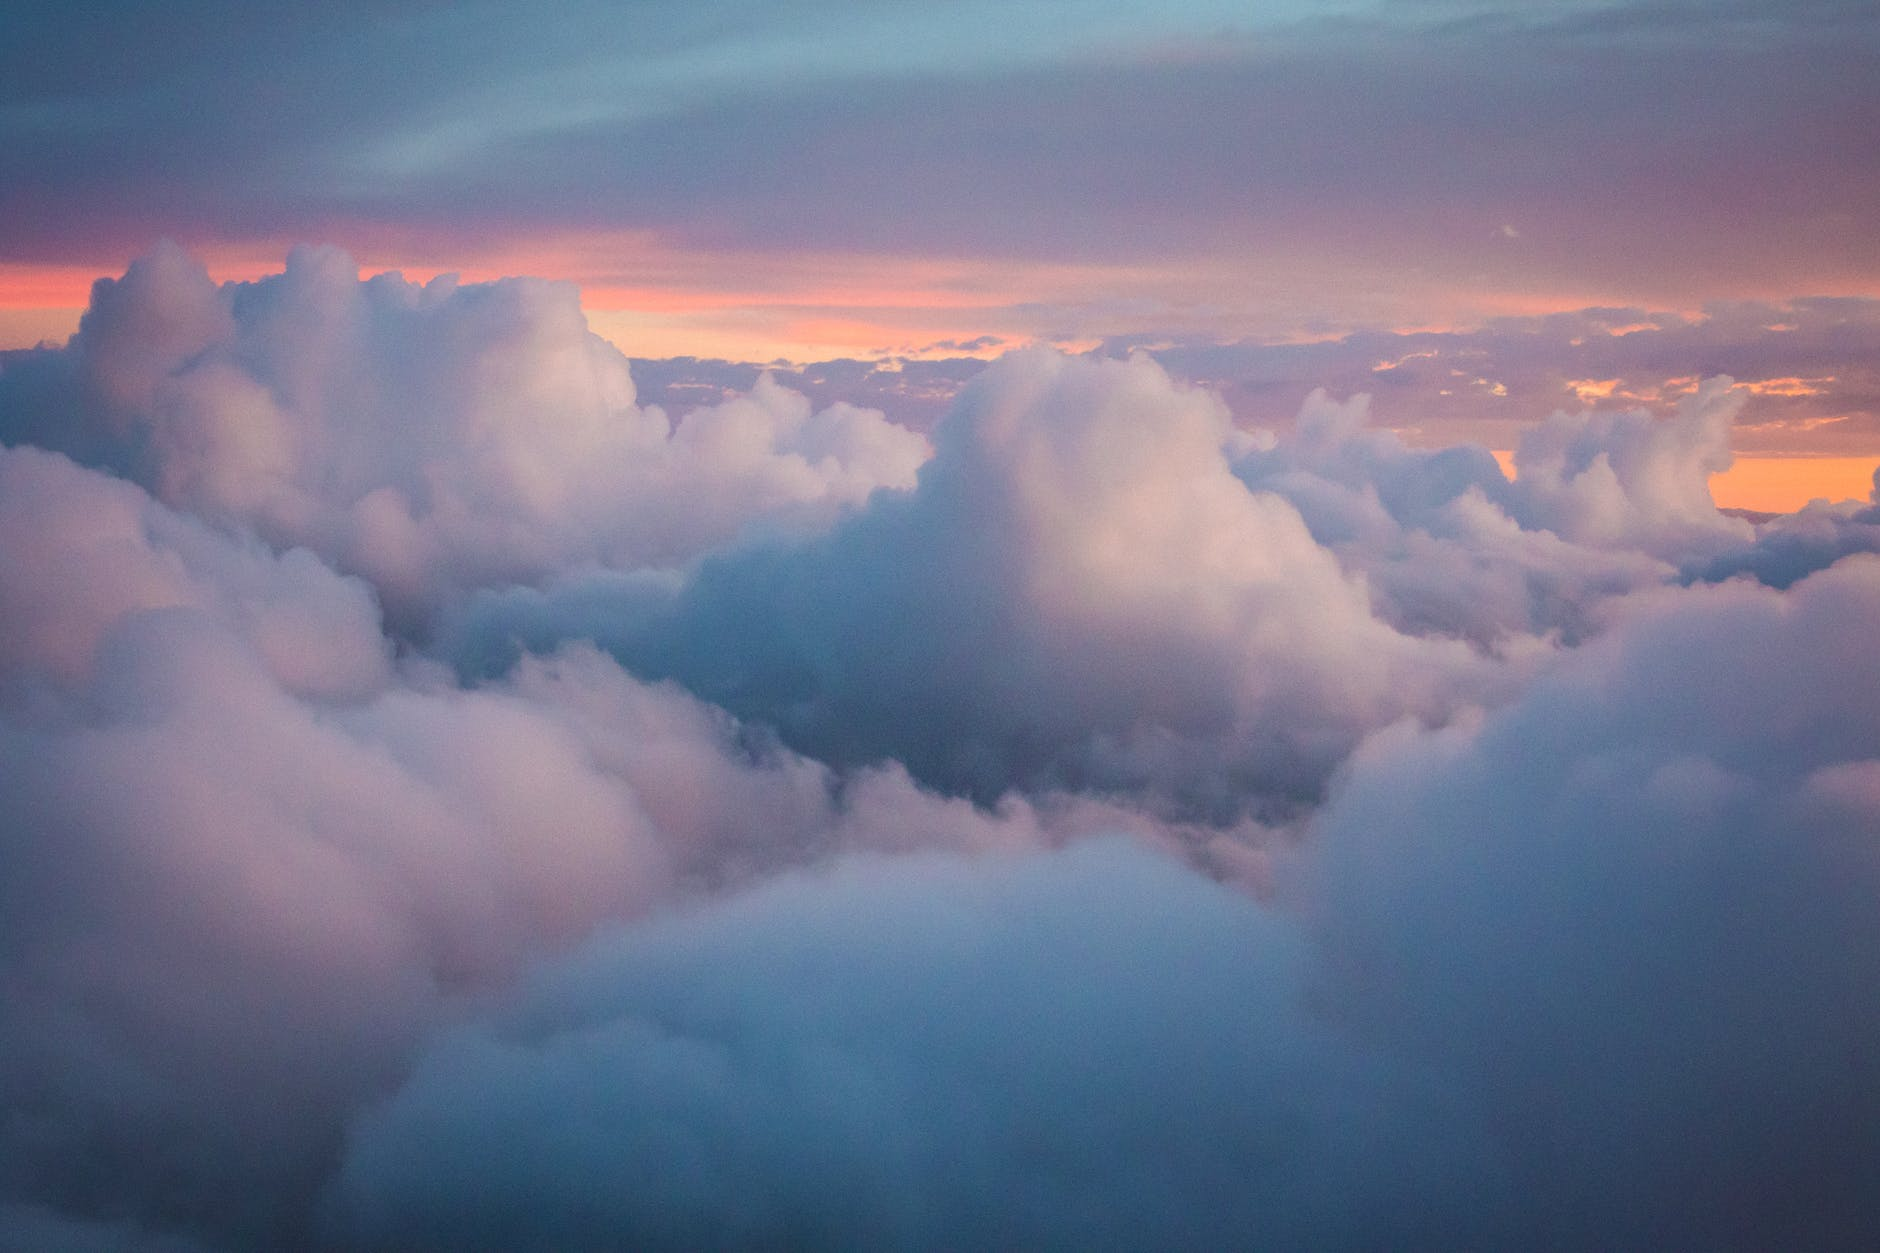
\includegraphics[height=3cm]{02_Introduction/images/clouds.jpg} %% Magda Ehlers
\hspace{0.01cm}
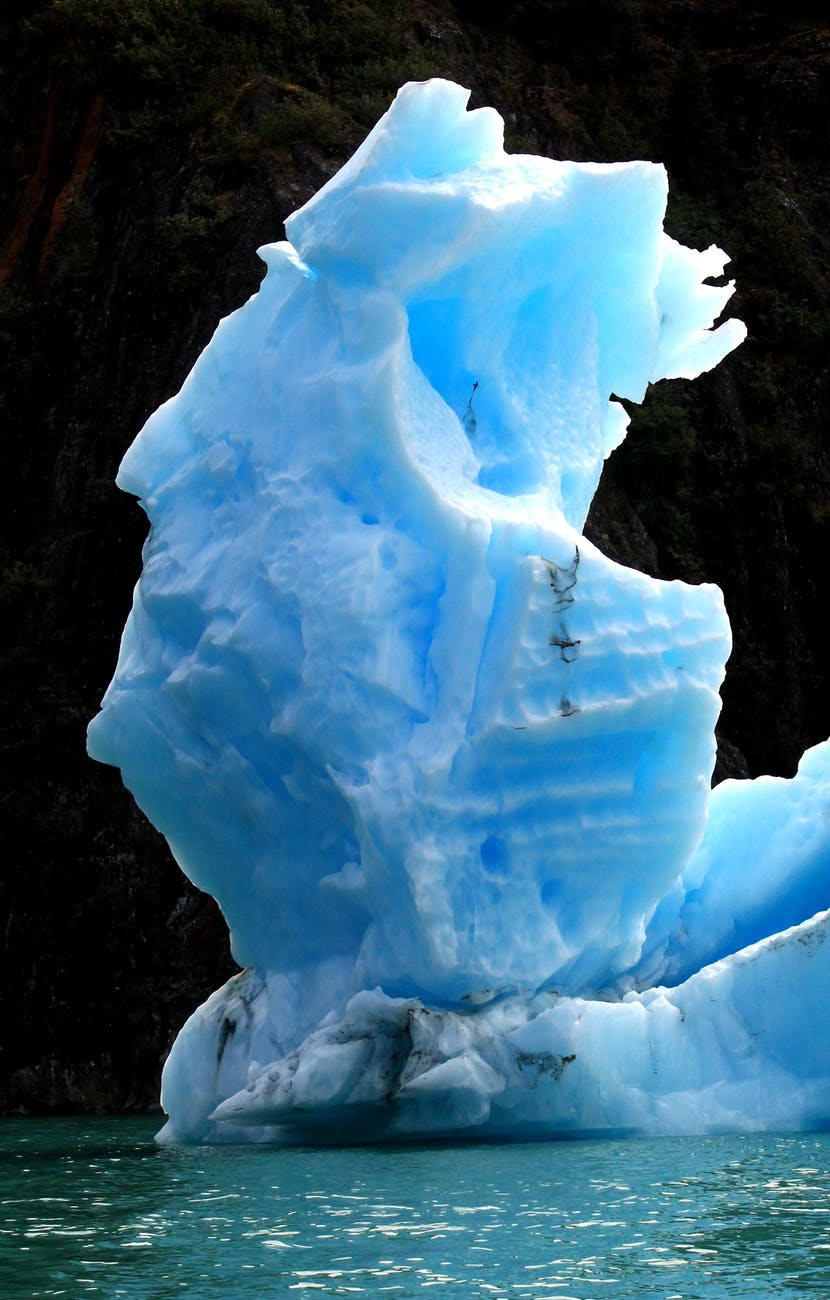
\includegraphics[height=3cm]{02_Introduction/images/iceberg.jpg} %% pixabay
\hspace{0.01cm}
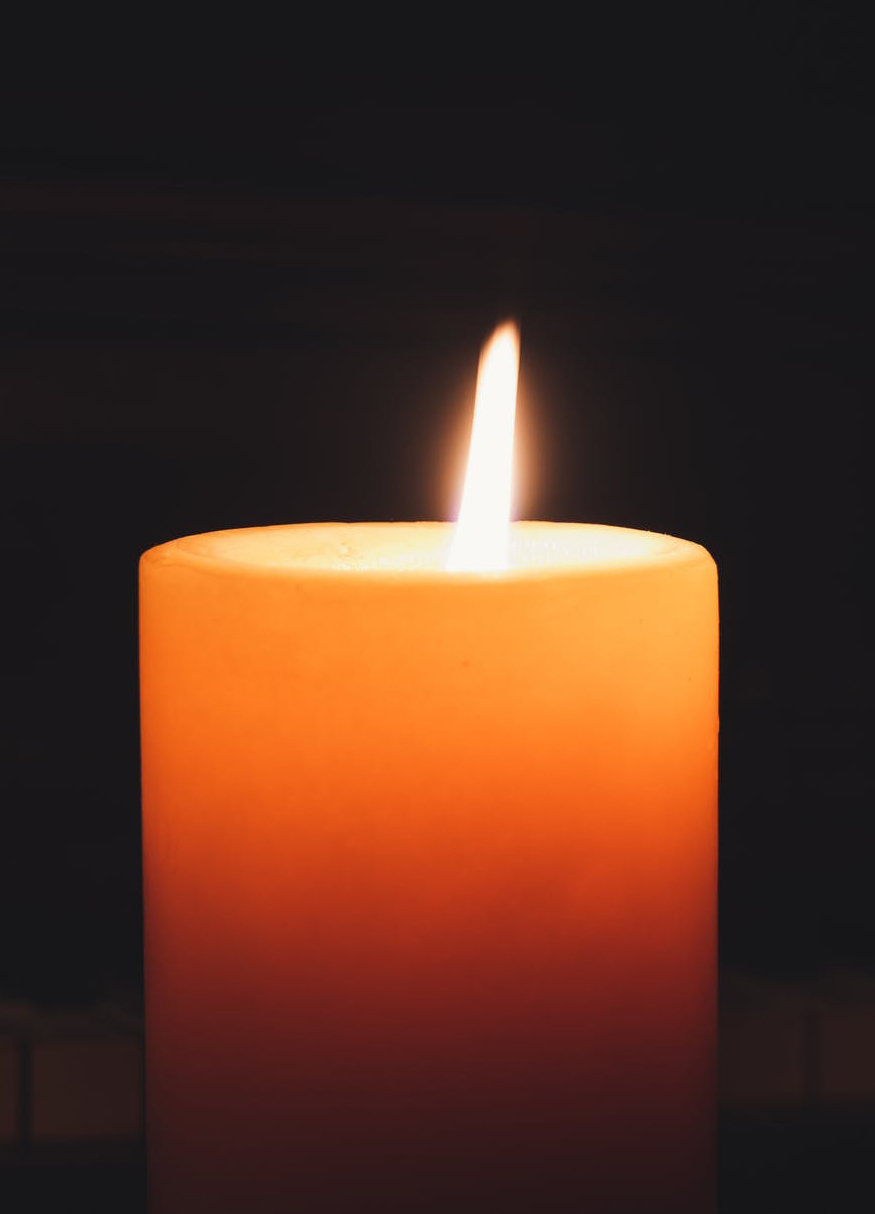
\includegraphics[height=3cm]{02_Introduction/images/candle.jpg} %% Brett Sayles
}
\end{center}
\caption{Real world examples of participating media. Reproducing these optical phenomena with computers requires resource intensive light transport simulations for which deterministic methods are developed in this thesis\protect\footnotemark.}
\label{fig:intro_participating_media_examples}
\end{figure}

Computer generated imagery (CGI) is used widely across many domains and industries such as architecture, entertainment, advertising, automotive, manufacturing and scientific visualization, where each brings its own challenges with it. This high demand and wide adoption is why rendering in computer graphics is a heavily researched subject in industry and academia alike. The main challenge research in rendering is trying to address is the high amount of computation current algorithms require in order to generate realistic images. For example a single frame in an animation movie by Disney or Pixar takes multiple hours on average and much more in extreme cases. To produce all images for the whole movie, multiple computing centers with thousands of CPU cores are used, which requires substantial economical investments. One of the main efforts in rendering research therefore is to reduce the computational cost for realistic image generation.\footnotetext{Photos provided under Creative Commons CC0 license by  Magda Ehlers (clouds), pixabay (iceberg), Brett Sayles (candle).}

The advent of graphics computing hardware has paved the way for realtime applications. Here, together with some additional compromises in physical accuracy, incredible performance gains enable the generation of images in fractions of seconds and are the basis for new powerful interactive applications in the industries mentioned above. Finding methods that can generate results at interactive rates while allowing control or at least understanding of accuraccy losses, is another important research direction in graphics.

Computer hardware is ever-evolving---while for a long time most of the increase in compute power came from higher density semiconductor fabrication---this trend has almost come to an halt. Today the growth in compute power is driven by parallelization on multi- and manycore systems. These challenges impact current rendering algorithms which mostly do not play well to the intricacies of the underlying hardware. While some first steps are being made in this direction (see for example Eisenacher et al.~\cite{Eisenacher13}), designing rendering algorithms that fully exploit the potential of next generation multi- or manycore hardware has been proclaimed as one of the future challenges for rendering by industry leaders (see Fascione~\cite{Fascione15}).

This thesis seeks to address these problems by following a trend which has been spurred by the so called physical based rendering revolution in graphics (see Keller et al.~\cite{Keller15}). In the early days of computer graphics, limitations in compute power required the use of cheap ad-hoc methods and other tricks to facilitate efficient image generation algorithms. With the growth in computational power, techniques and methods based on accurate physical models have become increasingly feasible and started replacing older heuristical approaches. Rendering became concerned with energy conservation, the use of correct physical quantities for describing the virtual scene and quantifiable error to physically correct ground truth results. Consistently adopting the framework provided by optical physics allowed rendering researchers to much better investigate and compare with work in other fields attacking very similar problems. While graphics research has always drawn inspiration and methods from other scientific domanis, the ermergence of physical based rendering caused a significant increase in research work which is based on findings and theories from other domains. Physics provided a common language allowing much easier to talk across disciplines.

In this spirit, this thesis investigates theories and methods from the astrophysics domain and nuclear sciences and adopts them for application in rendering. The resulting work presented in this thesis addresses all the three challenges mentioned above. Specifically, methods are presented which allow to reduce computational cost for the demanding problem of rendering participating media such as clouds, smoke, fire etc. and even allows---with some compromise in accuracy---applications at interactive rates. The methods devised in this thesis turn the rendering problem into the problem of solving a linear system of equations, exactly what high performance computing clusters (large scale many-core systems) have been designed for (see Koerner et al.~\cite{Koerner17}). This thesis constitutes a significant effort in putting forward an alternative approach to light transport simulation which has not seen a lot of attention lately but might have the potential to answer some of the reseach challenges in rendering today and tomorrow.

%\TD{visualization}
%\TD{inverse rendering}

\section{Research Questions}

This thesis is concerned with rendering volumetric media such as clouds, fire, milk and fog which interacts with light. These participating media elements are ubiquitous in the real world and therefore also common in rendering. Todays standard methods in rendering work by tracing particles of light (photons) through the scene. These particles interact with the scene and form complex trajectories from light sources to the sensor of the virtual camera which captures the image. Participating media such as clouds or milk cause particularly long trajectories for light particles and therefore are computationally very demanding. This is specifically extreme for media like clouds or milk where the particle trajectories become excessively long.


The problem of tracing particles through a participating medium involving many particle interactions with long trajectories is not exclusive to light particles in computer graphics. Very similar problems exist in nuclear science for example, when computing the dosis of radiation leaving the protected core of a nuclear power plant. Here, high-energy neutrons are traced from the reaction through the surrounding wall, which acts as a participating medium (e.g. Haghighat et al.~\cite{Haghighat03}). In astrophysics, for example, the study of the formation of planets (which apparently to this day is not fully understood) has models that take the radiation of stars into account, and the associated simulation therefore requires tracing particles that are emitted from fusion through clouds of debris and dust (see Armitage et al.~\cite{Armitage11}).

Common to all these different problems is the migration and interaction of particles or energy within a host medium. This is being described by linear transport theory, a field in mathematical physics which is at the intersection between astrophysics, nuclear sciences and computer graphics.
\begin{figure}[ht]
\centering
%\missingfigure{linear transport as intersection between astrophysics nuclear sciences computer graphics }
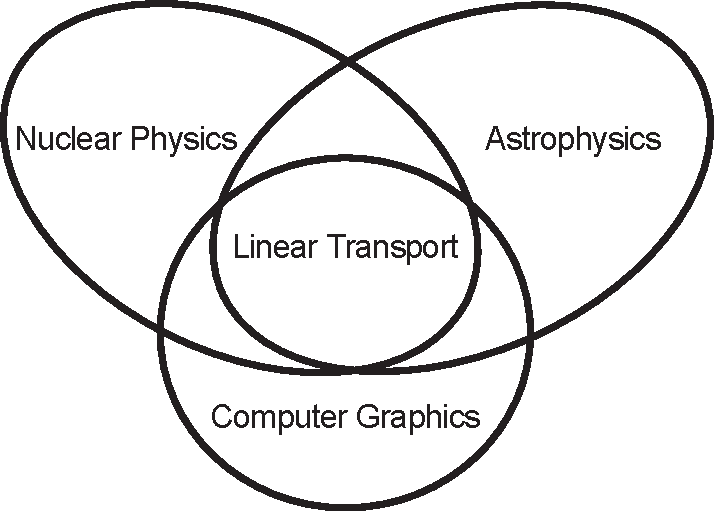
\includegraphics[width=0.6\textwidth]{02_Introduction/figures/fig_linear_transport.pdf}
\caption{Light transport simulation for rendering in graphics shares problems with other domains such as astrophysics and nuclear sciences. This thesis draws ideas from the long history of research done in those fields and inspires new methods for application in graphics.}
\label{fig:intro_linear_transport_fields}
\end{figure}

Now astrophysics and nuclear sciences have a much longer standing history than computer graphics and a lot of research was done before modern computers were widely available. This led to a large volume of work in those fields dealing with very similar problems in graphics from a very different perspective. As a result there are many interesting ideas, methods and techniques to find which could be benefitial for applications in computer graphics.

D'Eon~\cite{DEon14} in his work explains vividly the challenges this type of research comes with. Starting with notation and terminology which makes it difficult to read and understand papers from these fields. Further many seminal texts from those other domains are out of print, expensive to aquire, lack offical digital distribution formats and generally are hard to find. Since much of academic research was published before modern computers became a commodity, most publications focus exclusively on theoretical treatments and simple one-dimensional or two-dimensional problems. Practical computational methods are lacking and simply were not focus of research back then. New methods will have to be devised after going through the literature and putting the puzzle pieces together. However, doing this type of translational research can lead to powerful new tools in graphics. Significant recent advances, such as the work by D'Eon et al.~\cite{dEon11}, Vorba et al.~\cite{Vorba16} or Krivanek et al.~\cite{Krivanek14} are based to a large degree on old methods which were invented in other scientific domains.

The work in this thesis follows the same spirit. The $P_N$-method (see Brunner~\cite{Brunner02}) is a very popular method in nuclear sciences. It allows to compute a global solution without using the computational demanding standard method of following particle trajectories. The classical diffusion approximation (see~Ishimaru~\cite{Ishimaru78}) is a method which is used in the astrophysics domain and actually has been introduced to graphics by Stam~\cite{Stam95}. However an extension to flux-limited diffusion was introduced in the astrophysics domain by Levermore et al.~\cite{Levermore81} and has not been introduced to graphics yet. What all these different methods unify is the fact that they are based on a model that uses the same discretization.

The central research question this thesis will explore is whether these methods have merit for applications in computer graphics, and how they could be adopted to typicall problems in rendering. This consists of two parts. First the theory needs to be revisited and presented to a computer graphics audience. How is the theory derived from first order principles? Is it applicable for applications in rendering? What are the theoretical limitations and how do they affect the scope of applications? Second, modern and efficient methods need to be derived which allow application in a typical computer graphics context. How can the theoretical problem be solved for a typical application in rendering? How could a practical and efficient method look like? What shortcomings does it have and how could those be overcome?

\section{Summary of Original Contributions}

The research which was carried out as part of this thesis resulted in two major contributions which are based on $P_N$-method research in nuclear sciences and flux-limited diffusion in the astrophysics domain. In both cases practical methods for full three-dimensional problems did not exist and had to be devised, resulting in original published contributions in its own right.

\textbf{$P_N$-Method for Multiple Scattering in Participating Media~\cite{Koerner18}} The first contribution is a novel deterministic method for solving the $P_N$-equations on a finite difference grid for applications in rendering. The $P_N$-theory is derived and presented for a computer graphics audience. An original side product is a very concise and compact form of the real-valued $P_N$-equation which is new to the whole literature on $P_N$-based methods. The devised method introduced in this thesis is based on the idea of automated discretization. This approach works not only for the $P_N$-equations, but also for arbitrary potentially coupled PDE's and therefore has potential to be of interest for other applications and problems in graphics. This publication was inspired by research which was also carried out as part of this thesis on using high performance computing for application in rendering (\textbf{High-Performance Computing for Artistic Content Creation}~\cite{Koerner17}).

\textbf{Flux-limited Diffusion for Multiple Scattering in Participating Media~\cite{Koerner14}} The second contribution is a new and efficient method for computing the contribution of multiple scattered light in participating media. The method is based on flux-limited diffusion theory which is being derived and presented for a computer graphics audience. The moment closure problem and variable Eddington factors are introduced and a non-linear Gauss-Seidel method is devised to solve it. Furthermore, the results and performance traits are compared against $P_N$-method and classical diffusion approximation to give a clear understanding about the merits of each method.

Finally an additional contribution of this thesis is the clear and detailed discussion of the theory behind deterministic methods based on the spherical harmonics discretization of the linear transport equation. Additionally, the classical diffusion approximation are derived and a multigrid method for solving it is presented, making this thesis a comprehensive treatment on the subject.

The candidate also pursued another set of topics during his studies---while these resulted in a peer-reviewed publication \textbf{Subdivision Next-Event Estimation for Path-Traced Subsurface Scattering}~\cite{Koerner16}---they are only tangentially related to the body of this thesis and therefore not discussed.

\section{Organization of the Dissertation}

At the core of this thesis are chapters~\ref{sec:pnmethod} and \ref{sec:fld}. Each chapter is related to one of the methods which can be derived from the spherical harmonics discretization of the underlying transport equation and contains a detailed derivation of the theory behind the method the chapter is dedicated to. Then in each chapter a method for solving the respective equation is devised. These core chapters are complemented with a chapter on the foundations on light transport simulation (chapter~\ref{sec:foundations}). This section gives the radiative transfer equation and outlines the main approaches for solving it. Stochastic methods are introduced briefly and contrasted against deterministic methods to which spherical harmonics based discretizations covered in this thesis belong to. Finally the thesis closes with chapter~\ref{sec:conclusion} that reiterates over major conclusions from the three core chapters and identifies future directions for research. Figure~\ref{fig:intro_organization} gives a visual overview over the structure of this thesis.
\begin{figure}[ht]
\hspace{0.1\columnwidth}
%\centering
%\missingfigure{organizational structure thesis}
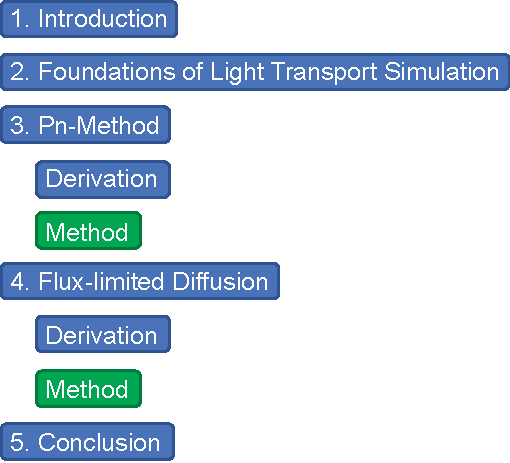
\includegraphics[width=0.6\textwidth]{02_Introduction/figures/fig_organigram.pdf}
\caption{Organigram of this thesis showing original contributions in green.}
\label{fig:intro_organization}
\end{figure}









\chapter{Foundations of Light Transport Simulation}
\label{sec:foundations}

This chapter gives an overview of light transport simulation in the context of rendering in computer graphics and specifically reviews the family of deterministic spherical harmonics based methods. After the introduction of the physical background and important terminology, a brief overview over the landscape of methods for solving light transport problems is given. This is divided into three sections as per the following categorization: analytical methods (section~\ref{sec:foundations_analytical}), stochastic methods (section~\ref{sec:foundations_mc}) and deterministic methods (section~\ref{sec:foundations_deterministic}).

The field of computer graphics is primarily concerned with the generation of images from virtual scenes as seen by a virtual camera. This requires to reproduce the emission of light and its interaction with the scene and the sensor. The study of the behavior of light is subject to optics, a separate branch of physics. Due to the intricate nature of light, a series of increasingly complex models exist, which can account for various properties. Fundamental to light is its particle-wave duality, which states that light can be described both, as individual particles (photons) or waves. Challenging to the subject is, that not all properties of light can be described by solely the particle nor the wave perspective. To account for all properties, both have to be considered and require quantum mechanics. The field of wave optics is based on a simpler model that can account for optical effects, caused by the wave property, such as interference and diffraction. The simplest model for light transport is provided by geometric optics, which models light as particle trajectories or rays and is referred to as ray optics. This model works well when the wavelength is small compared to the scene in which the light propagates. 

As the virtual (and real) camera is supposed to capture the image as closely as possible to human perception, the simulated wavelength of light is limited to the visible range of a human being (380 to 740 nanometers). Because this is very small compared to distances encountered in real world scenes, wave effects are of less importance and the model of geometric optics is sufficient most of the time. It is the basis for light transport simulation in graphics. This thesis is exclusively concerned with light transport in participating media i.a. clouds, smoke, fire, and water.


% ============================================================
\section{The Radiative Transfer Equation}

Geometric optics describes light as particles, that travel through the scene along straight lines between single interactions. At each interaction, the particle may change its course and continue to travel along another straight segment. When interacting with a medium, such as a cloud, each particle undergoes numerous interactions and creates long trajectories based on medium properties.

To derive a model that can explain this complex system of many particles interacting with the scene, a statistical approach is taken. Since photons carry energy, a collection of photons can be described by their collective energy. To express the propagation of photons, time is required. This is captured by the quantity flux $\psi$: it gives the amount of energy from all photons going through a surface within a time interval. It is given in Watts, which is specified in Joule (Energy) per second and depends on position $\vec{x}$ and direction $\vec{\omega}$:
\begin{align*}
\psi\left(\vec{x}, \vec{\omega}\right)
\quad
\left[\si{\watt} = \frac{\si{\joule}}{\si{\second}}\right]
\end{align*}

To find the flux for arbitrary surfaces (e.g. the camera sensor) and directions (e.g. the viewing direction of an observer), the radiance field $L$ is required. It captures the amount of light going through an infinitesimally small area and arriving from an infinitesimally small opening angle around a given direction $\vec{\omega}$. More precisely, it specifies the change of flux according to a change in direction $\vec{\omega}$ and a change in surface area that is projected onto a plane perpendicular to direction $\vec{\omega}$:
\begin{align*}
L\left(\vec{x}, \vec{\omega}\right) = \frac{\partial\partial\psi\left(\vec{x}, \vec{\omega}\right)}{\partial\vec{\omega}\partial A^\perp\left(\vec{x}\right)}
\quad
\left[\frac{\si{\watt}}{\si{\steradian}\, \si{\meter}^2}\right]
\end{align*}
The radiance field allows finding the amount of energy going through arbitrary surfaces and arbitrary angles by integration. This yields additional derivative quantities such as the fluence $\phi$, which integrates the radiance field over solid angle of the unit sphere at position $\vec{x}$:
\begin{align*}
\phi\left(\vec{x}\right) = \int_\Omega L\left(\vec{x}, \vec{\omega}\right) \ud\vec{\omega}
\quad
\left[\frac{\si{\watt}}{\si{\meter}^2}\right]
\end{align*}
It gives the total power of radiant energy arriving at position $\vec{x}$ gathered from all directions. Integrating the radiance field after projecting it onto the planes of the cartesian coordinate system, gives rise to the flux vector $\vec{E}$:
\begin{align*}
\vec{E}\left(\vec{x}\right) = \int_\Omega L\left(\vec{x}, \vec{\omega}\right)\vec{\omega} \ud\vec{\omega}
\end{align*}
The direction of the vector specifies the direction of bulk or dominant energy flow and the magnitude the net flux through an infinitesimally small surface, which is aligned to the direction.

The radiance field $L$ describes the distribution of photon densities in the scene and can easily be used to generate images by integrating it over the sensor surface of a virtual camera sensor and over all directions, from which photons can arrive on the sensor. This results in the energy that the sensor receives over a certain time (flux $\psi$).

%\TD{pixel color as integral over sensor surface}

However, the model needs to describe changes in the radiance field $L$ through changes in position. For this purpose, the directional derivative $\left(\vec{\omega}\cdot\nabla\right)L$ is used. It describes the rate of change of the radiance field $L$, when changing the position an infinitesimal step into direction $\vec{\omega}$.

\begin{figure}[h]
\centering
%\missingfigure{visualization of inscattering, outscattering and absorption.}
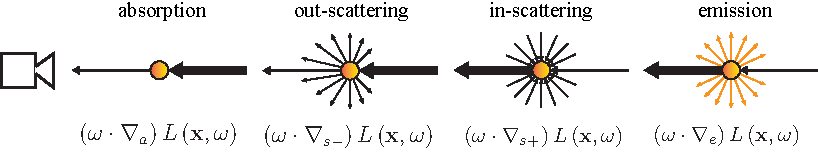
\includegraphics[width=1.0\textwidth]{03_foundations_of_light_transport_simulation/figures/fig_rte_terms.pdf}
\caption{Directional derivatives of the radiance $L$ along direction $\vec{\omega}$ model the interaction of light with participating media and constitue the radiative transfer equation.}
\label{fig:rte_change_L_all}
\end{figure}

The radiance field $L$ changes along direction $\vec{\omega}$ due to different optical phenomena, such as absorption, scattering and emission. Absorption models the effect of radiative energy being transformed into heat or kinetic energy. The amount of absorption depends on the medium and is controlled by the absorption coefficient $\sigma_a$. This value combines the number of absorbing particles in the medium as well as the collective surface area of their intersection with a hypothetical plane, which is oriented into the direction of change. The particles are assumed to be spherical or to have a random distribution of orientation. The coefficient controls the loss of energy due to absorption, when making an infinitesimal step along direction $\vec{\omega}$:
\begin{align}
\left(\vec{\omega}\cdot\nabla_{a}\right)L = -\sigma_a L\left(\vec{x}, \vec{\omega} \right)
\end{align}

Scattering describes collision of medium particles. Rather than being absorbed, they change their direction. This is controlled similarly to absorption by the scattering coefficient $\sigma_s$. Scattering has an effect on $L$ in two ways. Firstly, most of the scattering photons will change their direction away from the direction along which the rate of change of $L$, namely outscattering is measured:
\begin{align}
\left(\vec{\omega}\cdot\nabla_{s-}\right)L = -\sigma_s L\left(\vec{x}, \vec{\omega} \right)
\end{align}

Secondly, scattering affects the way the radiance field changes along $\vec{\omega}$ in that photons arriving from all directions will collide with the volume and scatter into the direction $\vec{\omega}$. This is called inscattering:
\begin{align}
\left(\vec{\omega}\cdot\nabla_{s+}\right)L = \sigma_s \int_{\Omega'}\phase\left(\vec{x}, \vec{\omega}'\cdot\vec{\omega}\right)L\left(\vec{x}, \vec{\omega} \right)\ud\vec{\omega}'
\label{eq:rte_inscattering}
\end{align}
The quantity $p$ is the phase function, a medium parameter, which determines how light is redistributed from an incident direction $\vec{\omega}'$ to the outgoing direction $\vec{\omega}$. Since medium particles are assumed to either be spherical or randomly oriented, this function does not change as both vectors $\vec{\omega}_i$ and $\vec{\omega}$ are rotated, and therefore, the cosine of the angle between the two vectors suffices as a parameter.

%\todo[inline]{phase function}
%\todo[inline]{isotropic phase function}
%\todo[inline]{anisotropic phase function}
%\todo[inline]{mean cosine}
%\begin{align}
%\label{eq:foundations_mean_cosine}
%X
%\end{align}

Finally, the radiance field changes along direction $\vec{\omega}$, due to the medium emitting photons itsself into direction $\vec{\omega}$. This is modelled by a source term $Q_e$:
\begin{align}
\left(\vec{\omega}\cdot\nabla_{e}\right)L = Q_e\left(\vec{x}, \vec{\omega}\right)
\end{align}

All terms combined produce the radiative transfer equation (RTE), which expresses the change of the radiance field $L$, with respect to an infinitesimal change of position in direction $\vec{\omega}$ at point $\vec{x}$ due to absorption, scattering and emission:
\begin{align}
\left(\nabla\cdot\vec{\omega}\right)L\left(\vec{x}, \vec{\omega} \right)
=&
-\sigma_t\left(\vec{x}\right) L\left(\vec{x}, \vec{\omega} \right)\nonumber\\
&
+\sigma_s\left(\vec{x}\right) \int_{\Omega}
{
\phase\left(\vec{\omega}'\cdot\vec{\omega}\right)L\left(\vec{x}, \vec{\omega}' \right)\ud\vec{\omega}'
}
\label{eq:rte}
\\
&
+Q_e\left(\vec{x}, \vec{\omega}\right)
\nonumber
\  .
\end{align}
where $\sigma_t=\sigma_a+\sigma_s$ is the extinction coefficient, which combines absorption and outscattering.

The radiative transfer equation, as presented, is based on important key assumptions about the modelled light transport (D'Eon~\cite{DEon14}):
\begin{itemize}
\item Linear transport: levels of heat, created by the absorption events don't measurably change the properties of the medium itself. Further photons do not collide with each other and therefore, the transport equation remains linear.
\item Steady-state: It is not of relevance to know how light propagates through the scene over time. The typical exposure times of cameras or the human visual system is in a regime, where it is safe to assume that sinks and sources are constant in time and are balanced out in an equilibrium state, such that the radiance field $L$ does not change over time.
\item Monoenergetic: often referred to as gray problems. Light is assumed to have a single frequency and color is introduced by solving the single frequency problem multiple times for color space primaries.
\item Energy-conserving media: the medium will never scatter more energy at any point, than it receives.
\item Scalar radiative transfer: polarization of light is not considered.
\item Uncorrelated interaction events: particles have no memory and the probability distribution of an interaction event does not depend on the previous interaction in any way (Moon et al.~\cite{Moon07}).
\item Isotropic medium: the medium is assumed isotropic, which means that absorption and scattering coefficients are not direction dependent and the phase function only depends on the cosine of the angle between incident and outgoing direction (Jakob et al.~\cite{Jakob10}).
\end{itemize}

For notational convenience and for developing the theory for deterministic methods, the radiative transfer equation is expressed in operator notation where transport, collision, and scattering are operators $\mathcal{T}$, $\mathcal{C}$ and $\mathcal{S}$, being applied to the radiance field $L$:
\begin{align}
\mathcal{T}\left(L\right) &= -\mathcal{C}\left(L\right) + \mathcal{S}\left(L\right) + Q_e
\label{eq:rte_operator_notation}
\\
\mathcal{C}\left(L\right) &= \sigma_t\left(\vec{x}\right) L\left(\vec{x}, \vec{\omega} \right)
\nonumber
\\
\mathcal{S}\left(L\right) &= \sigma_s \int_{\Omega'}\phase\left(\vec{x}, \vec{\omega}'\cdot\vec{\omega}\right)L\left(\vec{x}, \vec{\omega} \right)\ud\vec{\omega}'
\nonumber
\\
Q_e &= Q_e\left(\vec{x}, \vec{\omega}\right)
\nonumber
\end{align}

Light transport simulation is the process for finding the solutions to $L$, either for specific values of $\vec{x}$ and $\vec{\omega}$ or globally. The following section gives an overview of the three main categories of methods for solving the radiative transfer equation, of which the last covers deterministic methods and leads into the subject of this thesis. The next section briefly covers analytical solutions which are popular and have been used to great effect. Section~\ref{sec:foundations_mc} covers stochastic methods, such as the Monte Carlo method. These methods will be introduced to motivate the need for deterministic methods as a potential means that boosts convergence of stochastic techniques. The last section introduces deterministic methods and covers how discretization of spatial and angular variable leads to a linear systems of equations.

% ============================================================
\section{Analytical Solutions}
\label{sec:foundations_analytical}

Analytical solutions to the radiative transfer equation exist for some very basic canonical problems, of which the point source problem is the most popular. It assumes a homogeneous medium (spatially constant $\sigma_t$) with an infinite extent. For this problem, a correct analytical solution exists (D'Eon et al.~\cite{dEon11}). D'Eon also introduced a very accurate approximation by Grosjean~\cite{Grosjean56}, which is simpler to evaluate and convergent. This analytical solution will be used to verify the various methods developed as part of this thesis.

Pegoraro et al.~\cite{Pegoraro11} introduced a method based on the analytical solution to the point source problem for application in realtime rendering of single scattered light in participating media (termed airlight integral).

Jensen et al.~\cite{Jensen01} introduced the diffusion theory and in particular the analytical solution to the diffusion approximation for the point source problem (theoretical treatment in chapter~\ref{sec:diffusion_approximation}). Besides, the authors introduced the method of images, which yielded an analytical solution to the half space problem. This problem consists of two different homogeneous media, which are separated by a plane of infinite extend (creating a half space). A solution to the half space problem allowed to locally approximate light transport at the surface of a bounded participating media, using a dipole configuration(termed subsurface scattering). Dipole based analytical models gained popularity in academia and industry and represented a rich and heavily researched branch within rendering. Further seminal work on this subject after Jensen was provided by D'Eon et al.~\cite{dEon11} and Habel et al.~\cite{Habel13}.

The main drawback of analytical models is their restriction to simple problems and homogeneous media in particular. Also, they introduce in some cases significant error, when the canonical problem is used on geometry that violates the plane-parallel assumption. Further dipole methods are based on the diffusion theory, which has poor directional resolution and complications with energy conservation (see section~\ref{sec:moment_problem_revisited}).

% ============================================================
\section{Stochastic Methods}
\label{sec:foundations_mc}

For most practical applications, analytical solutions do not exist, and numerical integration is required. The key challenge with solving the radiative transfer equation using numerical integration is the global nature of $L$. Changing a scene parameter in one place will affect all other parts in the scene. This global dependency is introduced by the integral over the radiance field in the scattering term. 

Naively integrating the scattering term by using common quadrature rules that are based on interpolation functions on a regular grid (e.g. Riemann integration) becomes prohibitively expensive with one or two recursion levels already as the function evaluations grow exponentially with the number of recursions, known as the \emph{curse of dimensionality}. An alternative to interpolation based-quadrature is Monte Carlo integration based on random samples. This is the core principle behind all stochastic methods.

The following sections provide a very brief overview of standard Monte Carlo methods for various reasons: First, it will help to differentiate deterministic methods, which are introduced later. Second, it explains how the ground truth images used in the result sections of chapter~\ref{sec:pnmethod}, chapter~\ref{sec:diffusion_approximation}, and chapter~\ref{sec:fld} were generated. Furthermore, the introduced methods in this thesis require computation of the single scattered light contribution, for which stochastic methods are used. Last, this section intends to inspire research in combining stochastic methods with deterministic methods into hybrid approaches, combining the benefits of both worlds and by this motivates research into deterministic methods in general.

\subsubsection*{Distributed Ray Tracing}

The invention of Monte-Carlo integration is attributed to Stanislaw Ulam who devised the idea in 1946 during his work on the Manhatten project in the Los Alamos National Lab (Metropolis~\cite{Metropolis49, Metropolis87}). Consider a function $f\left(x\right)$ for which the following integral over domain $\mathbb{R}$ needs to be found:
\begin{align}
\int f\left(x\right)\ud x
\label{eq:mc_integral_1}
\end{align}
The key idea is to turn the argument $x$ of a function $f(x)$ into a random variable. A stochastic process for randomly choosing instances of $x$ augments each individual value of $x$ with a probability density $p(x)$ and turns the set of all possible $x$ into a measure $\mu(x)$.

With $x$ being a random variable, $f\left(x\right)$ becomes a random variable itsself for which statistical moments can be computed. In particular the expected value can be computed by integrating over the measure $\mu(x)$ and weighting the results of $f$ with the probabilty for sampling $x$:
\begin{align}
E\left[f\right] = \int_{\mu\left(x\right)} f\left(x\right)p\left(x\right)\ud\mu\left(x\right)
\end{align}
The probability of sampling $x$ is implicitly given by the function $p$ which in turn is driven by the sampling method chosen. Since sample $x$ represents an infinitely small point in the continuous space $\mu\left(x\right)$ a probability can not be assigned directly the same way mass can not be assigned to an infinitely small particle (the particle can always be seen to be smaller than any mass value assigned to it). This is why $p(x)$ returns a probability \emph{density} (probability mass per probability volume) for a specific sample $x$. Probabilities can be found by integrating probability density $p$ over elements in subsets of $\mu\left(x\right)$.

The key idea behind Monte Carlo integration is to turn the computation of the expected value into the computation of the integral in equation~\ref{eq:mc_integral_1}. This is done by introducing a new function $g$ which cancels out the term $p\left(x\right)$:
\begin{align}
E\left[g\right]
=E\left[\frac{f\left(x\right)}{p\left(x\right)}\right]
= \int_{\mu\left(x\right)} \frac{f\left(x\right)}{p\left(x\right)}p\left(x\right)\ud\mu\left(x\right)
=\int f\left(x\right)\ud x
\end{align}
The power of Monte-Carlo integration as a numerical algorithm comes with that the expected value\mydash and therefore the sought integral\mydash can be estimated by the arithmetic mean over a set of $N$ random samples of $x$. This estimate is denoted by the operator $\left<\cdot\right>_N$:
\begin{align}
\left<E[g]\right>_N = 
\frac{1}{N}\sum_{i=0}^{N}
g\left(X_i\right)
\end{align}
This relation is derived from the law of large numbers which states that the average of the results obtained from $N$ number of trials of an experiment approaches its expected value as $N$ increases (see standard textbooks such as Karlos et al.~\cite{Kalos86}):
\begin{align}
\lim_{N\rightarrow\infty} \left<E[g]\right>_N = E[g]
\end{align}
For numerical procedures a finite number of samples is used which introduces some error in the estimate. The estimation error shows up as noise when using independent random samples to compute the radiance field estimates on the camera sensor for each pixel.

Naively using the Monte-Carlo integration technique with the inscattering integral (see equation~\ref{eq:rte_inscattering}) gives rise to distributed raytracing and was developed by Cook et al.~\cite{Cook84}. It allowed unbiased rendering of complex effects such as motion blur and depth of field but did not address the curse of dimensionality. Recursing the radiative transfer equation would still cause exponential growth of evaluations with each interaction, depending on the number of samples $N$.


% path tracing --------------------------------------------
\subsubsection*{Path Tracing}

The rendering equation is an integral equation which describes the propagation of light in scenes without any participating medium. Instead of applying Monte-Carlo directly to the in-scattering integral of the rendering equation and integrating over solid angle, Veach~\cite{VeachThesis97} proposed to reformulate the equation as an integral over all possible paths of photons which start from the place of emission (light sources) and arrive at position $\vec{x}$ from direction $\vec{\omega}$ to contribute to $L(\vec{x}, \vec{\omega})$. This laid the foundation of the path integral formulation which is the underlying framework used by all Monte-Carlo techniques in rendering today. Pauly et al.~\cite{Pauly00} then later applied this to the radiative transfer equation which opened up the use of Monte Carlo techniques for light transport simulation in participating media.


The path integral framework introduces the concept of a path $\bar{\mathrm{x}}$ which represents the trajectory a photon can make by traveling from where it was emitted to some position $\vec{x}$ with some incident direction $\vec{\omega}$. The path $\bar{\mathrm{x}}$ consists of $N$ vertices $\vec{x}_i$ at which interaction events occur. The function $f\left(\bar{\mathrm{x}}\right)$ takes such a single path as input and returns the contribution which a photon makes to $L(\vec{x}, \vec{\omega})$ after being emitted with initial energy $L_e$ from the light source and traveling along the path trajectory represented by $\bar{\mathrm{x}}$ accounting for all the terms in the radiative transfer equation~\ref{eq:rte} which reduce energy along the way.
\begin{figure}[t]
\centering
%\missingfigure{path sample and contribution factors}
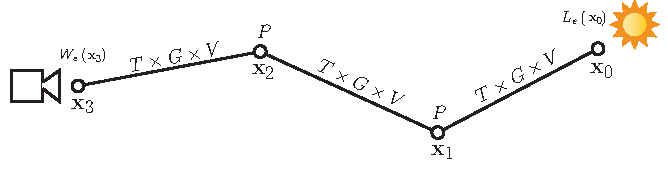
\includegraphics[width=1.0\textwidth]{03_foundations_of_light_transport_simulation/figures/fig_path_sample.pdf}
\caption{Path sample and its contributing factors to energy loss of radiant energy from the light source to the sensor.}
\label{fig:mc_path_sample_contributions}
\end{figure}

Energy is reduced for each segment $\vec{x}_i \vec{x}_{i+1}$ by the geometry term $G$ which results from the change in the projected area, the transmittance term $T$ which accounts for absorption and outscattering and the visibility term $V$ which accounts for geometry obstructing the path alltogether. At each interior path vertex $\vec{x}_i$, scattering is accounted for by multiplying with phase function term $P(\vec{x}_{i-1}, \vec{x}_i, \vec{x}_{i+1})$. Finally an importance weight $W_e$ accounts for sensor sensitivity.
\begin{align}
\hspace{-.3in}
f\left(\bar{\mathrm{x}}\right) =
L_e\left(\vec{x}_0\right)
W_e\left(\vec{x}_N\right)
\prod_{i=0}^{i=N-1}
G\left(\vec{x}_i, \vec{x}_{i+1}\right)
T\left(\vec{x}_i, \vec{x}_{i+1}\right)
V\left(\vec{x}_i, \vec{x}_{i+1}\right)
\prod_{i=1}^{i=N-1}
P\left(\vec{x}_{i-1}, \vec{x}_i, \vec{x}_{i+1}\right)
\label{eq:foundations_mc_pathintegral}
\end{align}
The transmittance is defined as
\begin{align}
T\left(\vec{x}_i, \vec{x}_{i+1}\right) =
\operatorname{exp}^
{
    -\int_{\vec{x}_i}^{\vec{x}_{i+1}}\sigma_t\left(\vec{x}\right)\ud\vec{x}
}
\end{align}
and the geometry term is defined as
\begin{align}
G\left(\vec{x}_i, \vec{x}_{i+1}\right) =
\frac{D\left(\vec{x}_{i}, \vec{x}_{i+1}\right)D\left(\vec{x}_{i+1}, \vec{x}_{i}\right)}{\norm{\vec{x}_{i+1}-\vec{x}_{i}}^2} \,,
\end{align}
where
\begin{align}
D\left(\vec{a}, \vec{b}\right) =
\begin{cases}
\abs{\vec{n}_a\cdot\vec{\omega}_{ab}}, & \text{if $\vec{a}$ is a surface vertex}
\\
1, & \text{if $\vec{a}$ is a volume vertex}
\end{cases}
\end{align}
Here $\vec{n}_a$ is the normal at the surface vertex $\vec{a}$ and $\vec{\omega}_{ab}$ is the normalized direction vector pointing from vertex $\vec{a}$ to vertex $\vec{b}$.

The last term is defined in terms of the volume phase function $\phase$ and the surface scattering function $\phase_s$:
\begin{align}
P\left(\vec{x}_{i-1}, \vec{x}_i, \vec{x}_{i+1}\right) =
\begin{cases}
\phase_s\left(\vec{\omega}_{x_ix_{i-1}}\cdot\vec{\omega}_{x_ix_{i+1}}, \vec{n}_i\right), & \text{if $\vec{x}_i$ is a surface vertex}
\\
\phase\left(\vec{\omega}_{x_ix_{i-1}}\cdot\vec{\omega}_{x_ix_{i+1}}\right), & \text{if $\vec{x}_i$ is a volume vertex}
\end{cases}
\end{align}
This thesis exclusively deals with participating media and therefore surface scattering is of no concern.

The set $\mu\left(\bar{\mathrm{x}}\right)$ is the set of all possible photon trajectories which arrive at $\vec{x}$ from direction $\vec{\omega}$ and start at any light source in the scene. Each sample is assigned a probability density $p\left(\bar{\mathrm{x}}\right)$ according to a sampling method. Light transport simulation aims to find a solution for $L(\vec{x}, \vec{\omega})$. With the path integral formulation this can be expressed as a Monte-Carlo integral over path space:
\begin{align}
L\left(\vec{x},\vec{\omega}\right) = E[g] = \int_{\mu\left(\bar{\mathrm{x}}\right)} \frac{f\left(\bar{\mathrm{x}}\right)}{p\left(\bar{\mathrm{x}}\right)}p\left(\bar{\mathrm{x}}\right)
\ud\mu\left(\bar{\mathrm{x}}\right)
\end{align}
This can be estimated using a finite number of samples $X_i$:
\begin{align}
\left<E[g]\right>_N = 
\frac{1}{N}\sum_{i=0}^{N}
g\left(X_i\right)
\approx
L\left(\vec{x},\vec{\omega}\right)
\end{align}
As mentioned above, the estimation error shows up as image noise (if random samples are independent). It can be shown formally that to reduce the amount of noise in half, four times the number of samples are needed (see Veach~\cite{VeachThesis97}). This means that for noise-free results a huge number of samples are needed\mydash a significant drawback of Monte-Carlo methods.

\subsubsection*{Variance Reduction}

Reducing the variance of Monte-Carlo estimators and therefore improving the convergence behavior is the goal of most of the research on stochastic rendering methods. The primary strategy for variance reduction is to reduce the deflection or range of values under the integral sign. This is because the variance is driven by the amount the integrated function value deviates from its mean over the integrated range.

There are two ways to reduce the amount of variation of the integrand around its mean value. First we adjust the sampling strategy such that the probability density function $p\left(x\right)$ correlates with $f\left(x\right)$ as closely as possible. Ideally, the probability density function is identical to $f$ up to a normalization factor $c$. This approach is called importance sampling:
\begin{align}
L = E[g] =
\int_{\mu\left(\bar{\mathrm{x}}\right)} \frac{f\left(\bar{\mathrm{x}}\right)}{p\left(\bar{\mathrm{x}}\right)}p\left(\bar{\mathrm{x}}\right)
\ud\mu\left(\bar{\mathrm{x}}\right)
\stackrel{p\left(x\right)=c f\left(x\right)}{=}
\frac{1}{c}\int_{\mu\left(\bar{\mathrm{x}}\right)} p\left(\bar{\mathrm{x}}\right)
\ud\mu\left(\bar{\mathrm{x}}\right) = \frac{1}{c}
\end{align}
Clearly, such a sampling strategy would have to know the solution $L$ in the first place and therefore is only of theoretical interest. However, if the sampling strategies can account for some factors within $f$, a significant improvement in variance can be made. Finding good sampling strategies is a vast research branch in its own right within Monte-Carlo based rendering methods. The simplest form is incremental path construction which starts with an initial vertex either on the light source (light path sampling) or the sensor (eye path sampling) and incrementally samples additional points from which additional path segments are constructed. The random decisions are taken according to the terms in $f$ (see equation~\ref{eq:foundations_mc_pathintegral}). The probability density function is constructed by chaining the conditional probabilities for each decision made along the path. This causes the probability density function to respect individual terms and better correlate with the final contribution. 

However, sampling according to individual terms does not respect the product of those terms and therefore is not optimal. This is a continuing subject of research. The basic incremental path sampling was extended by Lafortune et al.~\cite{Lafortune93} and Veach et al.~\cite{Veach94} to bi-directional path-tracing. Here two paths are constructed incrementally. One starts at the light source and the second at the camera sensor. From these two paths, multiple individual full paths were constructed and their contribution combined in order to reduce variance. This concept was later generalized by Veach et al.~\cite{Veach95MIS} into multiple importance sampling. It allowed combining different Monte-Carlo estimators optimized for different light transport aspect. This spurred an explosion of research into sampling techniques and strategies.

Instead of incrementally sampling local terms such as phase function and geometry term to construct the next path vertex, globally informed sampling techniques appear to be a promising avenue. These techniques work by using an approximation to the radiance field function for importance sampling and therefore produce a better variance reduction than just using local information at each path vertex. Methods differentiate in their caching datastructure (Gaussian-Mixture Models are used by Vorba et al.~\cite{Vorba14} and an adaptive spatial-directional tree datastructure by M\"{u}ller et al.~\cite{Mueller17}) and the way these caches are bootstrapped (update from Monte-Carlo samples during rendering is done by Vorba et al.~\cite{Vorba14} and reinforcement learning is used by M\"{u}ller et al.~\cite{Mueller17}). These methods are a strong motivation for the use of fast approximative solutions from deterministic methods which are the topic of this thesis. Instead of using expensive unbiased Monte-Carlo samples which are then discretized into a cache datastructure, an approximate solution from a deterministic method could be used to quickly learn the skeleton of light transport in the scene and bootstrap the cache.

The second popular variance reduction technique for Monte-Carlo path tracing is based on control variates. Here the idea is to reduce the deflection of the integrand by using a closed form solution $C$ of an approximation $c\left(x\right)$ to the function $f\left(x\right)$:
\begin{align}
L &= E[g] =
\int_{\mu\left(\bar{\mathrm{x}}\right)}
\frac{f\left(\bar{\mathrm{x}}\right)-c\left(\bar{\mathrm{x}}\right)}{p\left(\bar{\mathrm{x}}\right)}p\left(\bar{\mathrm{x}}\right)
\ud\mu\left(\bar{\mathrm{x}}\right)
+C\left(\vec{x}, \vec{\omega}\right)
\\
C\left(\vec{x}, \vec{\omega}\right) &= 
\int_{\mu\left(\bar{\mathrm{x}}\right)}
c\left(\bar{\mathrm{x}}\right)
\ud\mu\left(\bar{\mathrm{x}}\right)
\end{align}
In the ideal case of $c=f$ the integral becomes zero and the equation reduces to $L=C$. Again this would require a closed-form solution of the original problem which does not exist. However, if $c$ correlates well with $f$, variance can be reduced. If no closed-form solution for $C$ exists, it can also be integrated numerically using Monte-Carlo integration. Applying the control variates to the integration of $C$ in such a nested fashion yields multilevel Monte-Carlo methods which have not been applied in rendering yet. 

Control variates have been used for surface rendering by Mehta et al.~\cite{Mehta12} and Clarberg et al.~\cite{Clarberg08}. For rendering of participating media, control variates have been applied successfully by Pegoraro et al.~\cite{Pegoraro08} where individual samples are used to create and update an adaptive cache of the discretized five-dimensional radiance field. This is very similar to the path-guiding techniques mentioned earlier with the difference that here the guiding cache is used as a control variate instead of a sampling function in the estimator. This work is likewise a good motivation for the deterministic methods developed as part of this thesis. Instead of building the cache from unbiased Monte-Carlo samples and introducing error by discretization into a cache datastructure, an approximation from deterministic methods could be used to bootstrap the cache.

More advanced variance reduction techniques work by better exploring the sample space $\mu\left(x\right)$. Markov-Chain-Monte-Carlo based methods start with a sample that has been generated using standard sampling and from there explore the sampling space by perturbation of that single sample. This concept has been further extended with Hamiltonian Monte-Carlo, where newton dynamics are used to generate trajectories which efficiently explore the important regions in high dimensional sample space. This requires sample space gradients which is a challenge due to the discontinuous visibility function. The coverage of these techniques is far beyond the scope of this thesis. The reader is referred to the work by Veach~\cite{VeachThesis97} and Cline et al.~\cite{Cline05, Cline05apractical} as a starting point into Markov-Chain-Monte-Carlo and the work by Li et al.~\cite{Li15} as an entry point into the use Hamiltonian Monte-Carlo for rendering.

The growth in computing power and the never ending need for more realistic imagery played into the fact that Monte-Carlo methods much better deal with higher dimensions and can produce an unbiased result. As in other fields, Monte-Carlo methods are now the gold standard for light transport simulation in computer graphics and improving their convergence is the primary research challenge.

The variance reduction techniques have been presented in this section because they show that having an approximation of the radiance function could be used with importance sampling and control variates to reduce the variance of Monte-Carlo estimators. This is a strong motivation for the use of fast approximative solutions from deterministic methods which will be discussed in the next section and are the topic of this thesis.


% hybrid methods
% Premože et al. proposed a sound mathematically-based version of this approach in the form of the most probable paths most probable (MPP) [PAS03, PAT+04] (bothours thesis p.87) \cite{Premoze04}
%\todo[inline]{Anton Bouthours stuff}
% granular media stuff to show the coupling between diffusion and monte carlo

% hybrid methods: path guiding
% russian roulette and splitting \cite{Vorba16}
% importance sampling \cite{Mueller17}
% propose deterministic methods as initial guide (discuss discretization etc.)



%\todo[inline]{explain the concept of variance}
%\todo[inline]{explain the concept of bias}
%\subsection{Variance Reduction Techniques}
%\label{sec:variance_reduction_techniques}
%\todo[inline]{Explain, that a great variety of Monte Carlo methods exist because there are many ways information and assumptions can be combined with the basic variance reduction techniques available for monte carlo integration}
%\todo[inline]{Local variance reduction technique}
%\todo[inline]{semi-global reduction technique}
%\todo[inline]{global reduction technique}
%\subsubsection{Importance Sampling}
%\todo[inline]{explain importance sampling basics}
%\todo[inline]{multiple importance sampling}
%\todo[inline]{explain JIS as a semi-global technique}
%\todo[inline]{explain SNEE as a semi-global technique}
%\subsubsection{Control Variates}
%\todo[inline]{explain control variates}
%\todo[inline]{multi-level monte carlo}
%\todo[inline]{residual ratio tracking (precomputing the maximum volume height for volume bricks as semi-global))}
%\subsubsection{Russian Roulette and Splitting}
%\todo[inline]{Point out, }
%\todo[inline]{Point out, that the different variance reduction techniques all }

% ============================================================
\section{Deterministic Methods}
\label{sec:foundations_deterministic}

Deterministic methods are based on the discretization of functions which depend on the continuous variables $\vec{x}$ and $\vec{\omega}$ into a discrete set of scalar values, that are flattened into a column vector $\vec{u}$. The discretization operator in the angular domain is denoted $\mathcal{P}_{\vec{\omega}}$ and the spatial discretization operator is expressed as $\mathcal{P}_{\vec{x}}$
\begin{align*}
L\left(\vec{x}, \vec{\omega}\right)
\xrightarrow[\mathcal{P}_{\vec{\omega}}]{\makebox[1cm]{}}
\xrightarrow[\mathcal{P}_{\vec{x}}]{\makebox[1cm]{}}
\vec{u}
\end{align*}
The discretization operators are also applied to the individual operators $\mathcal{T}$, $\mathcal{C}$ and $\mathcal{S}$, which constitute the radiative transfer equation, producing operator matrices $T$, $C$ and $S$ respectively:
\begin{align*}
\mathcal{T}
\xrightarrow[\mathcal{P}_{\vec{\omega}}]{\makebox[1cm]{}}
\xrightarrow[\mathcal{P}_{\vec{x}}]{\makebox[1cm]{}}
T
\\
\mathcal{C}
\xrightarrow[\mathcal{P}_{\vec{\omega}}]{\makebox[1cm]{}}
\xrightarrow[\mathcal{P}_{\vec{x}}]{\makebox[1cm]{}}
C
\\
\mathcal{S}
\xrightarrow[\mathcal{P}_{\vec{\omega}}]{\makebox[1cm]{}}
\xrightarrow[\mathcal{P}_{\vec{x}}]{\makebox[1cm]{}}
S
\end{align*}
If linear, these discretizations allow to express the application of the radiative transfer operators to the radiance field (see equation~\ref{eq:rte_operator_notation}) to be expressed in terms of matrix vector products:
\begin{align*}
T\vec{u}&=-C\vec{u}+S\vec{u}+Q
\\
T\vec{u}+C\vec{u}-S\vec{u}&=Q
\\
(T+C-S)\vec{u}&=Q
\\
A\vec{u}&=Q
\end{align*}
Deterministic methods turn the problem of solving the radiative transfer equation into the problem of solving a system of linear equations with the solution vector being a discretized version of the radiance field $L$.

The particular choice of $\mathcal{P}_{\vec{x}}$ and $\mathcal{P}_{\vec{\omega}}$ determines the concrete method used. For the spatial discretization $\mathcal{P}_{\vec{x}}$ a common choice in nuclear sciences are finite elements and hexagonal meshes in particular because it allows to best approximate solid geometry (e.g. from reactors) for boundary conditions. However, finite element discretization is unwieldy and difficult to setup. Throughout this thesis, we use a finite difference discretization which is very common in graphics and also easy to work within a practical context.
%https://en.wikipedia.org/wiki/Types_of_mesh
%\TD{talk about discretization and meshing}
%\todo[inline]{Spatial Discretization}
%\todo[inline]{Finite differences}
%\todo[inline]{Finite elements}

\subsubsection*{Spherical Harmonics Methods}
%PN
Using the spherical harmonics expansion for the discretization of the radiative transfer equation is a very popular approach in other fields, such as nuclear physics or astrophysics. Functions, that depend on the angular variable are turned into a discrete set of spherical harmonics coefficients. Likewise, the radiative transfer equation is turned into a coupled set of partial differential equations through spherical harmonics projection yielding the general $P_N$-equations. The underlying theory has its origins in astrophysics (see Brunner~\cite{Brunner02}) and is also popular in nuclear sciences (see Seibold et al.~\cite{Seibold14}) and medical science (see Frank et al.\cite{Frank08}). In computer graphics $P_N$-theory was discussed briefly in a paper by Kajia~\cite{Kajiya84} without any details on how to solve the equations. Max~\cite{Max95} pointed out, it is not clear if Kajiya succeeded at all at implementing a method for solving the $P_N$-equations, as all of the results in his paper were produced with a simpler approach\footnote{\cite{Max95} p.4: \emph{``[...] Kajiya attempted to solve these equations for the case of isotropic scattering, but it is unclear whether he succeeded, since all the pictures in \cite{Kajiya84} were produced by the simpler 'slab' method.[...]"}}. In the following chapter of this thesis, we derive the real-valued $P_N$-equations and present a new method for solving them on a finite difference grid. 

The $P_N$-theory has spurred the development of a rich variety of methods of which only the diffusion approximation has been introduced into the field of computer graphics (see Stam~\cite{Stam95}). It is derived as a degenerated case of the $P_N$-equations and gained a lot of popularity in graphics. Wang et al.~\cite{Wang08} applied diffusion to the problem of rendering subsurface scattering with heterogeneous participating media using finite elements. This approach was further extended to anisotropic media by Jakob et al.~\cite{Jakob10} who also used a more complex finite-element discretization in spatial domain. Arbree et al.~\cite{Arbree11} later in a similar approach addressed various problems in Wang's work and simplified discretization by using a tetrahedral mesh basis. Li et al.~\cite{Li13} used the same tetrahedral representation but a more efficient method for constructing the coefficient matrix which allowed realtime application under changing topology.

Another method, that is derived from the spherical harmonics expansion and can be seen as an extension to the classical diffusion approximation, is flux-limited diffusion. The theory has been invented in the astrophysics domain and is primarily attributed to Levermore et al.~\cite{Levermore81}. Zhang et al.~\cite{Zhang13}, similar to flux-limited diffusion, uses a combination of diffusion and advection to model light transport. In contrast to flux-limited diffusion, their approach was not derived formally from the radiative transfer equation. The scattering contribution is modelled with a diffusion term and a linear diffusion coefficient. This is not sufficient as we will see. It furthermore is restricted to time-dependent problems and uses a time stepping scheme involving alternating diffusion and advection steps using arbitrary time step and duration parameters. In chapter \ref{sec:fld} of this thesis we introduce flux-limited diffusion to the problem of rendering in computer graphics and present a new and efficient method for solving the flux-limited diffusion equation for steady-state radiative transfer.

Although classical diffusion already has been introduced to graphics, it is revisited in chapter~\ref{sec:diffusion_approximation} because its theory is important for the introduction of flux-limited diffusion and the multigrid diffusion solver presented has not been discussed in detail in the literature before.

\subsubsection*{Discrete Ordinate Method ($S_N$-Method)}
% SN
Instead of using the continuous spherical harmonics basis functions, an alternative approach for the discretization $\mathcal{P}_{\vec{\omega}}$ is to replace the continuous variable $\vec{\omega}$ by a discrete set of direction vectors $\vec{\omega}_i$ (e.g. using Gaussian quadrature points) which causes the inscattering integral (equation~\ref{eq:rte_inscattering}) to turn into a sum and in the end produces a system of linear equations. The variable $s$ is used to identify the direction vector, and the discrete directions are denoted $s_i$. This is why the method is also referred to as $S_N$-method (where $N$ is the number of directions). Development of the method is mostly attributed to Wick~\cite{Wick43} and Chandrasekhar~\cite{Chandrasekhar60}, who derived the $S_N$-method in one dimension. Later, Carlson et al.~\cite{Carlson61} extended the method to two and three dimensions. For the one-dimensional case, it has been shown, that $S_{N+1}$-theory is equivalent to $P_N$-theory, if Gaussian quadrature points are used (see~\cite{Cullen01}). In this case, the discrete $S_N$-directions correspond to the zero crossings of the Legendre polynomials used in $P_N$. In two or three dimensions however, this correspondence is broken and causes non-physical results, such as the ray effects for which the $S_N$-method is known for. These are discretization artifacts of the angular variable and appear as unphysical concentrated beams of light within the volume.
\begin{figure}[h]
\centering
\begin{subfigure}{0.4\columnwidth}
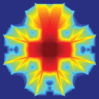
\includegraphics[width=\columnwidth]{03_foundations_of_light_transport_simulation/figures/sn_ray_effects.png}
\end{subfigure}%
\hspace{0.01\columnwidth}
\begin{subfigure}{0.4\columnwidth}

\includegraphics[width=\columnwidth]{03_foundations_of_light_transport_simulation/figures/sn_ground_truth.png}
\end{subfigure}%
\caption{This result from Camminady et al~\cite{Camminady2019} demonstrates the ray effects produced by the discrete ordinate method (left) in comparison to the ground truth (right) for the checkerboard problem. We also simulate the checkerboard problem for our methods (see \ref{sec:pn_results_checkerboard}).}
\end{figure}

Like the $P_N$-method, the $S_N$ method also has not been fully explored in the context of rendering in computer graphics yet. The most extensive investigations thereto were done by by Max~\cite{Max95}, who introduced a method for computing light propagation in participating media based on directional bins in a regular grid hence resembling the method of discrete ordinates.


\subsubsection*{Lattice-Boltzmann Method}

The Lattice-Boltzmann method was introduced by Geist et al.~\cite{Geist04} as an alternative to finite-element and finite difference methods for solving partial differential equations. The idea is to represent the particle distribution using a spatial grid. Transport is simulated by applying simple update rules to each grid cell in successive iterations. However, the method hardly gained traction, as there is no directional resolution but only photon densities per grid cell.

\subsubsection*{Heuristical Methods}

The necessity of fast computation and the need for realtime performance in graphics gave rise to methods which have not been derived formally from radiative transfer and which take additional assumptions to allow further simplification.

Miller et al.~\cite{Miller12} present a method for computing multiple scattering in clouds, that separates the cloud into directly illuminated boundary parts facing the lightsource and a remaining indirectly illuminated part. The method operates in two steps: It first computes the distance function to the directly illuminated part for the whole dataset. This requires solving the Eikonal equation using the fast marching method (see~\cite{Tsitsiklis95}). Then it computes the amount of light reaching each point within the medium as a function of distance. While being a rough simplification, the method allows for fine control through customizable radiance-distance profiles.

Light Propagation Volumes by Kaplanyan et al.~\cite{Kaplanyan10} were originally developed for surface geometry only and have later been extended to participating media by Billeter et al.~\cite{Billeter12}. The scene is aligned with a regular grid where each voxel contains a truncated spherical harmonics expansion of the radiance field (similar to $P_N$). Light emission is computed from single scattered light using reflective shadow maps by Dachsbacher et al.~\cite{Dachsbacher05}. Indirect light is computed by an iterative method. For each iteration, the light at every voxel is distributed to all voxels in a local neighborhood. The exchange of light is computed for each neighboring voxel taking the projected surface area of voxel faces into account. The process of updating all neighboring voxels within a certain radius, using the light at the center voxel, has some resemblance of wavefronts being emitted from the voxel. Although the technique is not derived directly from radiative transfer, it became very popular with realtime rendering for its convincing results.

%\todo[inline]{mention isotropic medium, anisotropic medium}

\begin{figure}[t]
\centering
%\missingfigure{overview of all angular discretization methods.}
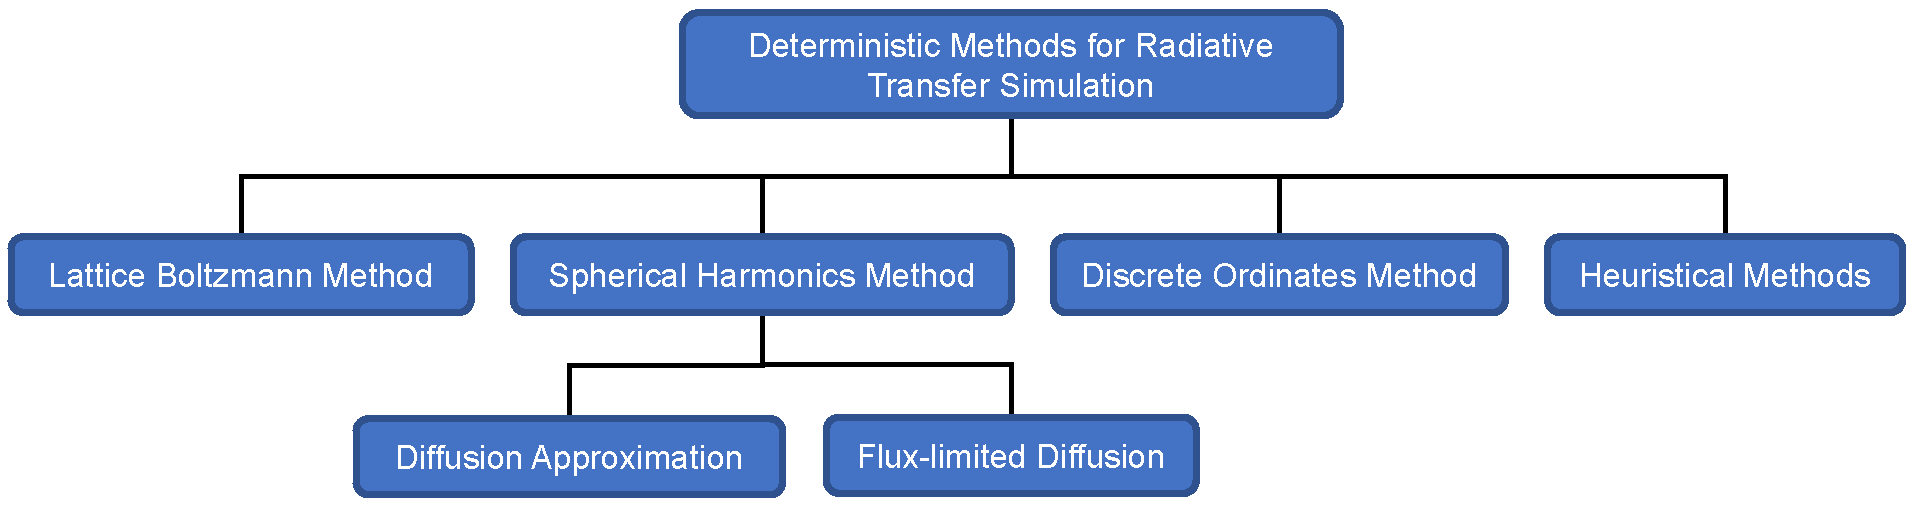
\includegraphics[width=1.0\textwidth]{03_foundations_of_light_transport_simulation/figures/fig_overview_methods.pdf}
\caption{Overview of deterministic methods for light transport simulation.}
\label{fig:rte_change_L_all}
\end{figure}

The benefits of deterministic methods generally are that they provide a noise-free solution for the complete radiance field $L$ throughout the whole domain. Their main drawbacks are their significant memory requirements for storing the representation of the five-dimensional radiance field function and the discretization error from spatial and angular discretization. Furthermore, deterministic methods tend to not be as general as Monte-Carlo methods and are limited to a subset of problems (e.g. isotropic phase functions). Additionally, some deterministic methods take a lot of time to converge to a solution in certain scenarios.

These drawbacks and the focus on accurate and unbiased Monte-Carlo methods have shifted attention away from deterministic methods lately. However, trends such as the path-guiding techniques discussed in section~\ref{sec:foundations_mc} motivate further research on deterministic methods, as they may be useful for bootstrapping guiding caches and therefore could lead to hybrid methods combining the best of both worlds. Consequently, this thesis investigates spherical harmonics methods, the branch of deterministic methods, which has seen most popularity in other domains, and tries to assess their merit for applications in rendering.


\chapter{$P_N$-Method for Multiple Scattering in Participating Media}
%
\label{sec:pnmethod}

The $P_N$-method presented in this chapter is a deterministic method for solving the radiative transfer equation. It is based on the spherical harmonics discretization of the radiative transfer equation and its related quantities in the angular domain. 

In this chapter,a thorough derivation of the $P_N$-theory will be given and a novel method for solving the underlying equations introduced. The first section introduces the spherical harmonics expansion and its important properties. The complex-valued $P_N$-equations are derived in section~\ref{sec:pn_cvalued}. The fact, that the radiance field is real-valued can be used to cut the number of unknown in half. This is done by using the real-valued $P_N$-equations. In section~\ref{sec:pn_rvalued}, a compact form of the real-valued $P_N$-equations is derived, which has not been given anywhere else in the literature. After a short note on two-dimensional problems in section~\ref{sec:pn_2d}, the chapter introduces a new method for solving the $P_N$-equations (section~\ref{sec:pn_solver}), closes by discussing its integration into a rendering framework and highlights results (section~\ref{sec:pn_results}).

% ============================================================
\section{Spherical Harmonics}
\label{sec:sh}

Spherical harmonics are the Fourier series for the sphere, and are an important tool for solving numerical problems involving the spherical domain. They are often derived as eigensolutions to the surface Laplacian, which is the analog to developing the Fourier series as eigensolutions of the operator $(d/dx)^2$ on a finite line with the boundary conditions that $y$ and $dy/dx$ match at the two ends (see Riley et al.~\cite{Riley2006}). The result of this derivation are complex-valued functions $\SHBC$, which are defined as:
\begin{align}
\label{eq:sh_definition}
\SHBC^{l,m}(\theta, \phi)=
\begin{cases}
C^{l,m}e^{im\phi}P^{l,m}\left(\operatorname{cos}\theta\right), & \text{for $m\ge0$}\\
\left(-1\right)^m\overline{\SHBC^{l\left|m\right|}}(\theta, \phi), & \text{for $m<0$}
\end{cases}
\quad ,
\end{align}
where $P^{l,m}$ are the associated Legendre polynomials. While those can be defined in many different ways, the most numerically robust way to evaluate them is by using the following set of recurrence relations (Press et al.~\cite{Press07}):
\begin{align}
P^{0,0}\left(\operatorname{cos}\theta\right) &=
1
\  ,
\nonumber
\\
P^{m,m}\left(\operatorname{cos}\theta\right) &=
\left(2m-1\right)!!\left(1-\operatorname{cos}^2\theta\right)^\frac{m}{2}
\  ,
\nonumber
\\
P^{m+1,m}\left(\operatorname{cos}\theta\right) &=
\operatorname{cos}\theta\left(2m+1\right)P^{m,m}\left(\operatorname{cos}\theta\right)
\ 
\nonumber
\\
P^{l,m}\left(\operatorname{cos}\theta\right) &=
\frac{\operatorname{cos}\theta\left(2l-1\right)}{l-m}
P^{l-1,m}\left(\operatorname{cos}\theta\right)
-
\frac{l+m-1}{l-m}
P^{l-2,m}\left(\operatorname{cos}\theta\right)
\  .
\label{eq:sh_Plm}
\end{align}
The factor $C^{l,m}$ in equation~\ref{eq:sh_definition} is defined as
\begin{align}
\label{eq:sh_definition_C}
C^{l,m}=(-1)^m\sqrt{\frac{2l+1}{4\pi}\frac{(l-m)!}{(l+m)!}}
\end{align}
Since spherical harmonics are used in many different fields, their definition can vary and one has to be careful, when comparing them across literature. This concerns the $(-1)^m$ factor in particular, which is called the Condon-Shortley phase. Sometimes, this factor is part of the definition of the associated Legendre polynomial $P^{l,m}$ and therefore does not appear in $C^{l,m}$. More importantly, the definition of $C^{l,m}$ depends on how the spherical harmonics are expected to be normalized.
\newline
\begin{figure}[h]
\centering
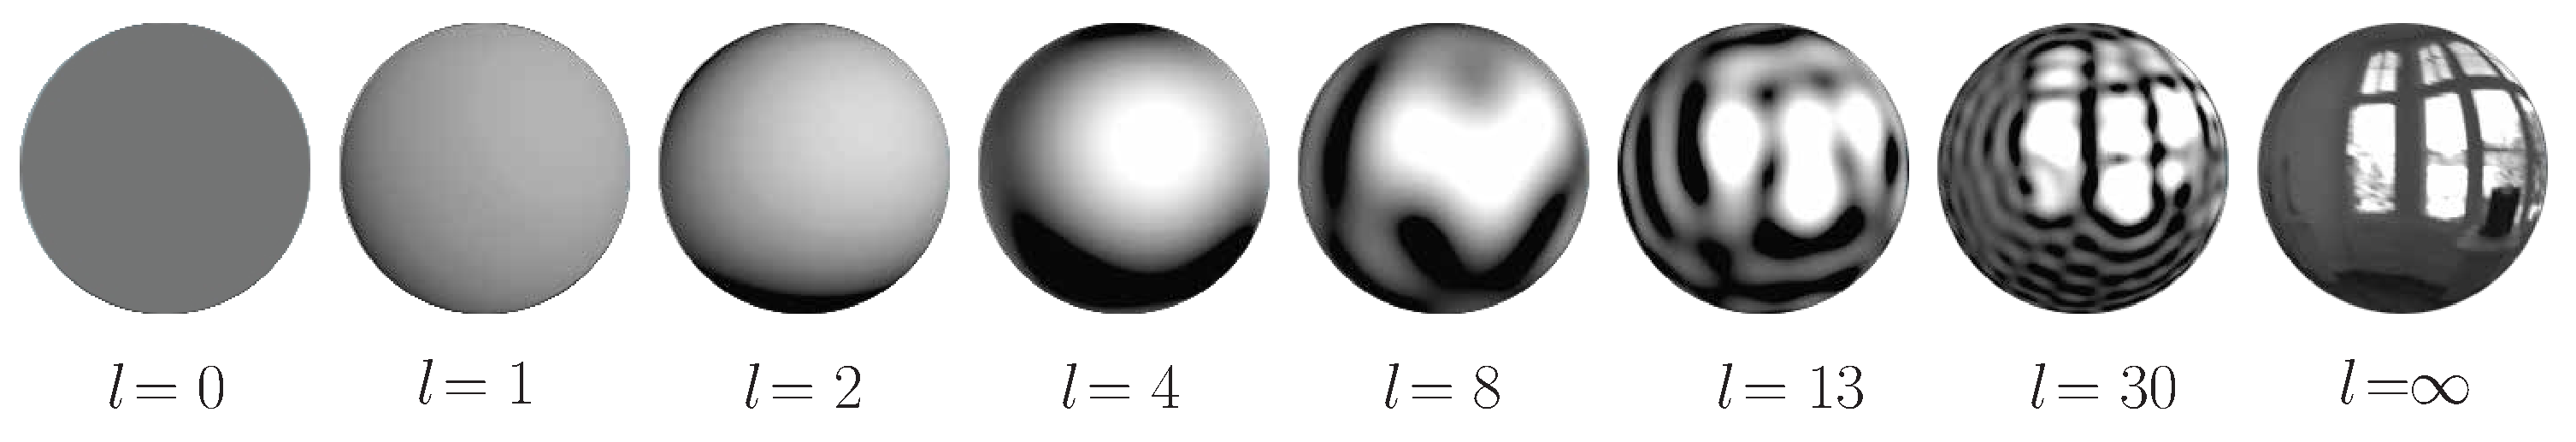
\includegraphics[width=\columnwidth]{04_pn_method/figures/fig_sph_frequencies.pdf}
\caption{Approximating a spherical function using spherical harmonics with increasing truncation order (from left to right). Like with the Fourier-transform, higher truncation order allows capturing higher frequencies.}
\label{fig:sh_vis}
\end{figure}


%\begin{figure}[h]
%\centering
%\begin{subfigure}{0.31\columnwidth}
%%\includegraphics[width=\columnwidth]{images/checkerboard2d_p1_neumann_staggered_starmap.png}
%%spherical harmonics basis function hierarchy in 2d
%\missingfigure{see comment}
%\caption{TODO}
%\label{fig:sh_vis_1}
%\end{subfigure}
%\hspace{0.01\columnwidth}
%\begin{subfigure}{0.31\columnwidth}
%%\includegraphics[width=\columnwidth]{images/checkerboard2d_p1_neumann_staggered.png}
%%some environment map and truncated reconstruction in 2d
%\missingfigure{see comment}
%\caption{TODO}
%\label{fig:sh_vis_2}
%\end{subfigure}
%\hspace{0.01\columnwidth}
%\begin{subfigure}{0.31\columnwidth}
%%\includegraphics[width=\columnwidth]{images/checkerboard2d_p1_neumann_staggered.png}
%%the hierarchy for the reconstruction with weights
%\missingfigure{see comment}
%\caption{TODO}
%\label{fig:sh_vis_3}
%\end{subfigure}%
%\caption{TODO}
%\label{fig:sh_vis}
%\end{figure}

\subsubsection*{Normalization and Orthogonality}

The coefficient $C^{l,m}$ has been defined as such that the spherical harmonics function $\SHBC$ scales to the unit norm
\begin{align}
\label{eq:sh_normalization}
\norm{\SHBC^{l,m}} = \sqrt{\left<\SHBC^{l,m}, \SHBC^{l,m}\right>} = 1
\ .
\end{align}
Other spherical harmonics definitions use a different constant (e.g. $4\pi$) and therefore arrive at different $C^{l,m}$. Since the spherical harmonics functions $\SHBC$ are complex-valued functions on the unit sphere, they are elements of the Hilbert space, for which the inner product is defined as:
\begin{align}
\label{eq:sh_inner_product}
\left<f,g\right> = \int_\Omega f\left(\vec{\omega}\right)\overline{g}\left(\vec{\omega}\right)\ud\vec{\omega}
\end{align}
with $\overline{g}$ being defined as the complex conjugate of $g$ (Folland~\cite{Folland92}).

The spherical harmonics functions form a orthogonal family and thus result in:
\begin{align}
\left<\SHBC^{l_1, m_1},\SHBC^{l_2, m_2}\right>
=
0
\ ,\quad\text{ for } l_1 \ne l_2 \text{ and } m_1 \ne m_2
\end{align}
The properties of normalization (equation~\ref{eq:sh_normalization}) and orthogonality (equation~\ref{eq:sh_orthogonality}) give
\begin{align}
\label{eq:sh_orthogonality}
\left<\SHBC^{l_1, m_1},\SHBC^{l_2, m_2}\right>=
\int_{\Omega} \SHBC^{l_1m_1}\left(\vec{\omega}\right) \overline{\SHBC^{l_2m_2}}\left(\vec{\omega}\right) \mathbf{d}\vec{\omega} = \delta_{l_1m_1}\delta_{l_2m_2}
\ .
\end{align}

\subsubsection*{Projection and Reconstruction}

Because the spherical harmonics are orthonormal, a spherical functional $f\left(\vec{\omega}\right)$ can be projected into scalar spherical harmonics basis function coefficients $f^{l,m}$, using the inner product from equation~\ref{eq:sh_inner_product}. For notational convenience the projection operator $\mathcal{P}$ shall be defined, which takes a spherical functional and returns its spherical harmonics projection for a given pair of spherical harmonics coefficients $l,m$:
\begin{align}
\label{eq:sh_projection}
\mathcal{P}^{l, m}(f) =  \left<f,\SHBC^{l, m}\right> = 
\int_\Omega f\left(\vec{\omega}\right)\overline{\SHBC^{l,m}}\left(\vec{\omega}\right)\ud\vec{\omega}
\ .
\end{align}
Note, the use of the complex conjugate $\overline{\SHBC}$ for computing the coefficients $f^{l,m}$. This comes from the definition of the inner product (equation~\ref{eq:sh_inner_product}), which is a result of Hilbert space theory. 

Given the coefficients $f^{l, m} = \mathcal{P}^{l, m}(f)$, the function $f$ can be fully reconstructed by summing up the weighted contributions from the spherical harmonics basis functions
\begin{align}
\label{eq:sh_reconstruction}
f\left(\vec{\omega}\right) = 
\sum_{l=0}^{N}
{
\sum_{m=-l}^{l}
{
f^{l,m}\left(\vec{x}\right)\SHBC^{l,m}\left(\vec{\omega}\right)
}
}
\ .
\end{align}
The function can be fully reconstructed if $N=\infty$. However, as with the Fourier-expansion, it is useful to truncate the expansion at a specific $N$ (giving $P_N$-method its name). This limits the number of coefficients at the expense of introducing an approximation error by cutting off higher frequencies. The number of sperical harmonics coefficients for truncation order $N$ is $(N+1)\times(N+1)$.

\subsubsection*{Frequency-invariant Rotation and Rotational Symmetry}

Applying a rotation to the argument of a spherical harmonics basis function of band $l$ can be expressed as a linear combination of spherical harmonics basis functions of the same order:
\begin{align}
\label{eq:sh_rotation}
\SHBC^{l,m}\left(R\vec{\omega}\right)=\sum_{j=-l}^{l}r^{l,j}\SHBC^{l,j}\left(\vec{\omega}\right)
\ .
\end{align}
This is derived from the fact that the spherical harmonics basis functions of order $l$ form an irreducible basis for the group of 3D-rotations (see Corollary $17.17$ in \cite{Hall13}). Equation~\ref{eq:sh_rotation} implies that a rotation of a function represented in spherical harmonics, does not introduce or loose any frequencies from or to other spherical harmonic bands and therefore is not subject to aliasing.

The spherical harmonics projection of a rotationally symmetric function $f$ simplifies to Zonal Spherical Harmonics, which are characterized by the fact that only coefficients with $f^{l,0}$ are needed for reconstruction. This property is needed for the derivation of the $P_N$-equations. In particular, the phase function depends only on the angle between incident direction $\vec{\omega}_i$ and outgoing direction $\vec{\omega}_o$, which means that the phase function will be rotationally symmetric around the outgoing direction, if it is fixed. 

A rotation $R(\alpha)$ of angle $\alpha$ around the pole axis is expressed in spherical harmonics as:
\begin{align*}
\rho_{R(\alpha)}(\SHBC^{l,m}) = e^{-i m\alpha}\SHBC^{l,m}
\ .
\end{align*}
If a function $f$ is rotationally symmetric around the pole axis, then following applies:
\begin{align*}
\rho_{R(\alpha)}(f) = f
\end{align*}
and in spherical harmonics this would be:
\begin{align*}
\sum_{l,m}
{
e^{-i m\alpha}
f^{l,m}
\SHBC^{l,m} }\left(\vec{\omega}\right)
=
\sum_{l,m}
{
\phase^{l,m}
\SHBC^{l,m}\left(\vec{\omega}\right)
}
\end{align*}
By equating coefficients this yields:
\begin{align*}
f^{l,m} = f^{l,m}e^{-i m\alpha}
\end{align*}
Since $e^{-i m\alpha}=1$ for all $\alpha$ only when $m=0$, the conclusion is that $f^{l,m} = 0$ for all $m\ne0$. For a function, which is rotationally symmetric around the pole axis, only the $m=0$ coefficients will be valid.

As mentioned earlier, this will be useful during the derivation of the $P_N$-equation and its scattering term in particular. If the outgoing direction $\vec{\omega}_o$ of the phase function at the north pole ($\vec{\omega}_o=\vec{e}_3$) is fixed, then the reconstruction requires exclusively the spherical harmonics coefficients with $m=0$:
\begin{align}
\label{eq:sh_exp_phase}
\phase(\vec{\omega}_i) =
\sum_l
{
\phase^{l0}
\SHBC^{l0}(\vec{\omega}_i)
}
\end{align}

\subsubsection*{Recursive Relation}

Another property, which will be important for the derivation of the $P_N$-equations and its derivative term in particular is the following recursive relation
\begin{equation}
\label{eq:recursive_relation}
\resizebox{1.0\hsize}{!}{$\vec{\omega}\overline{\SHBC^{l,m}} = \frac{1}{2}
\begin{pmatrix}
\ c^{l-1, m-1}\overline{\SHBC^{l-1,m-1}} - d^{l+1, m-1}\overline{\SHBC^{l+1,m-1}} - e^{l-1, m+1}\overline{\SHBC^{l-1,m+1}} + f^{l+1, m+1}\overline{\SHBC^{l+1,m+1}}\\
i\left(-c^{l-1, m-1}\overline{\SHBC^{l-1,m-1}} + d^{l+1, m-1}\overline{\SHBC^{l+1,m-1}} - e^{l-1, m+1}\overline{\SHBC^{l-1,m+1}} + f^{l+1, m+1}\overline{\SHBC^{l+1,m+1}}\right) \\
2\left(a^{l-1, m}\overline{\SHBC^{l-1,m}}+b^{l+1, m}\overline{\SHBC^{l+1,m}}\right)
\end{pmatrix}$}
\ ,
\end{equation}
where
\begin{equation*}
\resizebox{1.0\hsize}{!}{$
a^{l,m}= \sqrt{\frac{\left(l-m+1\right)\left(l+m+1\right)}{\left(2l+1\right)\left(2l-1\right)}} \qquad
b^{l,m}= \sqrt{\frac{\left(l-m\right)\left(l+m\right)}{\left(2l+1\right)\left(2l-1\right)}} \qquad
c^{l,m}= \sqrt{\frac{\left(l+m+1\right)\left(l+m+2\right)}{\left(2l+3\right)\left(2l+1\right)}}
$}
\end{equation*}
\begin{equation*}
\resizebox{1.0\hsize}{!}{$
d^{l,m}= \sqrt{\frac{\left(l-m\right)\left(l-m-1\right)}{\left(2l+1\right)\left(2l-1\right)}} \qquad
e^{l,m}= \sqrt{\frac{\left(l-m+1\right)\left(l-m+2\right)}{\left(2l+3\right)\left(2l+1\right)}} \qquad
f^{l,m}= \sqrt{\frac{\left(l+m\right)\left(l+m-1\right)}{\left(2l+1\right)\left(2l-1\right)}}
$}
\end{equation*}
This relation implies that a direction vector $\vec{\omega}$ scaled by a complex SH basis function $\SHBC$ of order $lm$ can be expressed as a vector of complex values basis functions of higher and lower order. Such recursion relations seem to be hard to find in the standard literature and are preserved through citations in relevant articles\footnote{according to email exchange with experts from nuclear sciences}, such as Seibold et al.~\cite{Seibold14} or Brunner et al.~\cite{Brunner05}. The signs for the $x$- and $y$- component depend on the handedness of the coordinate system, in which the spherical harmonics basis functions are defined.
\section{Complex-valued $P_N$-equations}
\label{sec:pn_cvalued}

Equipped with key properties of the spherical harmonics expansion, the complex-valued $P_N$-equations are derived in this section. The derivation follows two basic steps, which are executed separately on each term of the radiative transfer equation. The first step is to substitute each angular dependent radiative transfer quantity, such as the radiance field $L$, by its (truncated) spherical harmonics projection (equation~\ref{eq:sh_projection}). The second step is to apply the spherical harmonics projection to each term of the radiative transfer equation. This results in terms, which will depend on the spherical harmonics indices $l,m$ and therefore form a system of equations. The size of this system is driven by the truncation order $N$. The higher the value $N$, the higher frequencies in angular domain are taken into account for an approximation of the radiative transport.
% --------------------------------------------------------------
\subsubsection*{Transport Term}
The transport term of the RTE is given as
\begin{align*}
(\omega\cdot\nabla)L(\vec{x}, \omega)
\end{align*}
Replacing $L$ with its spherical harmonics expansion results in:
\begin{align*}
\left(\omega\cdot\nabla\right)
\left(
\sum_{l,m}
{
L^{l,m}\left(\vec{x}\right )
\SHBC^{l,m}\left(\omega\right)
}
\right)
\end{align*}
Next, the whole term is projected into spherical harmonics, which means a multiplication with $\overline{\SHBC^{l'm'}}$ and integration over solid angle:
\begin{align*}
\int_\Omega
{
\overline{Y^{l'm'}}(\omega\cdot\nabla)
\sum_{l,m}
{
L^{l,m}\left(\vec{x}\right)
\SHBC^{l,m}\left(\omega\right)
}
}
\ud\omega
\end{align*}
The spatial derivative can be extracted to get:
\begin{align*}
\nabla\cdot\int_\Omega
{
\omega\overline{\SHBC^{l'm'}}
\sum_{l,m}
{
L^{l,m}\left(\vec{x}\right)
\SHBC^{l,m}\left(\omega\right)
}
\ud\omega
}
\end{align*}
When applying the recursion relation (equation~\ref{eq:recursive_relation}) the following will be shown:
\begin{equation*}
\resizebox{1.0\hsize}{!}{$
\begin{pmatrix}
\frac{1}{2}\partial_x\\
\frac{i}{2}\partial_y\\
\partial_z
\end{pmatrix}
\cdot
\int_\Omega
\begin{pmatrix}
\ c^{l'-1, m'-1}\overline{\SHBC^{l'-1,m'-1}} - d^{l'+1, m'-1}\overline{\SHBC^{l'+1,m'-1}} - e^{l'-1, m'+1}\overline{\SHBC^{l'-1,m'+1}} + f^{l'+1, m'+1}\overline{\SHBC^{l'+1,m'+1}}\\
-c^{l'-1, m'-1}\overline{\SHBC^{l'-1,m'-1}} + d^{l'+1, m'-1}\overline{\SHBC^{l'+1,m'-1}} - e^{l'-1, m'+1}\overline{\SHBC^{l'-1,m'+1}} + f^{l'+1, m'+1}\overline{\SHBC^{l'+1,m'+1}} \\
a^{l'-1, m'}\overline{\SHBC^{l'-1,m'}}+b^{l'+1, m'}\overline{\SHBC^{l'+1,m'}}
\end{pmatrix}
\sum_{l,m}{
L^{l,m}\left(\vec{x}\right )\SHBC^{l,m}\left(\omega\right)
}
\ud\omega
$}
\end{equation*}
Integrating the vector term over solid angle, can be expressed as seperate solid angle integrals over each component. These integrals over a sum of terms are split into seperate integrals:
\begin{align*}
\begin{pmatrix}
\frac{1}{2}\partial_x\\
\frac{i}{2}\partial_y\\
\partial_z
\end{pmatrix}
\cdot
\begin{pmatrix}
\ c^{l'-1, m'-1}\sum_{l,m}{L^{l,m}\left(\vec{x}\right )\int_\Omega{\overline{\SHBC^{l'-1,m'-1}}\left(\omega\right)\SHBC^{l,m}\left(\omega\right)\ud\omega}} \quad - \quad ...\\
-c^{l'-1, m'-1}\sum_{l,m}{L^{l,m}\left(\vec{x}\right )\int_\Omega{\overline{\SHBC^{l'-1,m'-1}}\left(\omega\right)\SHBC^{l,m}\left(\omega\right)\ud\omega}} \quad + \quad ... \\
a^{l'-1, m'}\sum_{l,m}{L^{l,m}\left(\vec{x}\right )\int_\Omega{\overline{\SHBC^{l'-1,m'}}\left(\omega\right)\SHBC^{l,m}\left(\omega\right)\ud\omega}} \quad + \quad ...
\end{pmatrix}
\end{align*}
Applying the orthogonality property to the solid angle integrals will select specific $l,m$ in each term:
\begin{equation*}
\resizebox{1.0\hsize}{!}{$
\begin{pmatrix}
\frac{1}{2}\partial_x\\
\frac{i}{2}\partial_y\\
\partial_z
\end{pmatrix}
\cdot
\begin{pmatrix}
\ c^{l-1, m-1}L^{l-1,m-1} - d^{l+1, m-1}L^{l+1,m-1} - e^{l-1, m+1}L^{l-1,m+1} + f^{l+1, m+1}L^{l+1,m+1}\\
-c^{l-1, m-1}L^{l-1,m-1} + d^{l+1, m-1}L^{l+1,m-1} - e^{l-1, m+1}L^{l-1,m+1} + f^{l+1, m+1}L^{l+1,m+1} \\
a^{l-1, m}L^{l-1,m}+b^{l+1, m}L^{l+1,m}
\end{pmatrix}
$}
\end{equation*}
Which gives the final moment equation for the transport term:
\begin{align}
&
\frac{1}{2}c^{l-1, m-1}\partial_x L^{l-1,m-1}
-\frac{1}{2}d^{l+1, m-1}\partial_x L^{l+1,m-1}
-\frac{1}{2}e^{l-1, m+1}\partial_x L^{l-1,m+1}
\nonumber
\\
&
+\frac{1}{2}f^{l+1, m+1}\partial_x L^{l+1,m+1}
-\frac{i}{2}c^{l-1, m-1}\partial_y L^{l-1,m-1}
+\frac{i}{2}d^{l+1, m-1}\partial_y L^{l+1,m-1}
\nonumber
\\
&
-\frac{i}{2}e^{l-1, m+1}\partial_y L^{l-1,m+1}
+\frac{i}{2}f^{l+1, m+1}\partial_y L^{l+1,m+1}
+
a^{l-1, m}\partial_z L^{l-1,m}+b^{l+1, m}\partial_z L^{l+1,m}
\label{eq:sh_complex_transport}
\end{align}

% --------------------------------------------------------------
\subsubsection*{Scattering Term}

The scattering term in the RTE is given as:
\begin{align*}
\sigma_s(\vec{x})\int_{\Omega}\phase(\vec{x}, \omega'\cdot\omega)L(\vec{x}, \omega')\ud\omega'
\end{align*}
The phase function, used in isotropic scattering medium, only depends on the angle between incident and outgoing direction, and therefore is rotationally symmetric around the pole defining axis. This property allows to define a rotation $R(\omega)$, which rotates the phase function, such that the pole axis aligns with the outgoing direction vector $\omega$. This rotation is expressed as:
\begin{align*}
\rho_{R(\omega)}(\phase)
\ ,
\end{align*}
which can be implemented by applying the inverse rotation $R(\omega)^{-1}$ to the arguments of $\phase$. With this rotated phase function, the integral of the scattering operator can be expressed as a convolution:
\begin{align}
\int_{\Omega'}\phase(\vec{x}, \omega'\cdot\omega)L(\vec{x}, \omega')\ud\omega'
&=
\int_{\Omega'}{\rho_{R(\omega)}(\phase)(\operatorname{cos}\theta')L(\vec{x}, \omega')\ud\omega'}
\nonumber\\
&= \langle L,  \rho_{R(\omega)}(\phase)\rangle
\label{eq:complex_scatt_conv}
\end{align}
As the inner product integral of the convolution is evaluated, the phase function rotates along with the argument $\omega$.

Now, the spherical harmonics expansions of $L$ and $\phase$ (equation~\ref{eq:sh_exp_phase}) in the definition for the inner product of the convolution (equation~\ref{eq:complex_scatt_conv}) is used:
\begin{align*}
\langle L,  \rho_{R(\omega)}(\phase)\rangle = \left < \sum_{l,m}{L^{l,m}(\vec{x}) \SHBC^{l,m}}, \rho_{R(\omega)}\left ( \sum_{l}{\phase^{l0}\SHBC^{l0}} \right )\right>
\end{align*}
Due to linearity of the inner product operator, the non-angular dependent parts of the expansions can be pulled out:
\begin{align*}
\langle L,  \rho_{R(\omega)}(\phase)\rangle
&=
\sum_{l,m}
{
L^{l,m}(\vec{x})
\left<
\SHBC^{l,m},
\rho_{R(\omega)}
\left(\sum_l{\phase^{l0} \SHBC^{l0}}\right)
\right>
}
\end{align*}
and further:
\begin{align*}
\langle L,  \rho_{R(\omega)}(\phase)\rangle
&=
\sum_{l'}
{
\sum_{l,m}
{
\phase^{l'0}L^{l,m}(\vec{x})
\left<\SHBC^{l,m}, \rho_{R(\omega)}\left( \SHBC^{l'0} \right)\right>
}
}
\end{align*}
The rotation $\rho_{R(\omega)}$ of a function with frequency $l$ results in a function of frequency $l$ (equation~\ref{eq:sh_rotation}). In addition the spherical harmonics basis functions $\SHBC^{l,m}$ are orthogonal. Therefore following applies:
\begin{align*}
\left<
\SHBC^{l,m}, \rho_{R(\omega)}\left(\SHBC^{l'm'}\right)
\right> = 0       \qquad    \text{for all}\ \ l\ne l' 
\end{align*}
which further simplifies the inner product integral to:
\begin{align*}
\langle L,  \rho_{R(\omega)}(\phase)\rangle
&=
\sum_{l,m}
{
\phase^{l0}L^{l,m}(\vec{x})
\left<
\SHBC^{l,m}, \rho_{R(\omega)}\left(\SHBC^{l0} \right )
\right>
}
\end{align*}
What remains to be resolved is the inner product. The spherical harmonics basis functions $ \SHBC^{l,m}$ are eigenfunctions of the inner product integral operator in the equation above (Dai~\cite{Dai13}):
\begin{align*}
\left<
\SHBC^{l,m}, \rho_{R(\omega)}\left ( \SHBC^{l0} \right )\right> = \lambda_l \SHBC^{l,m}
\end{align*}
with
\begin{align*}
\lambda_l=\sqrt{\frac{4\pi}{2l+1}}
\end{align*}
Replacing the inner product leads to:
\begin{align*}
\langle L,  \rho_{R(\omega)}(p)\rangle
&=
\sum_{l,m}
{
\lambda_l
\phase^{l0}L^{l,m}(\vec{x})
\SHBC^{l,m}
}
\end{align*}
This allows to express the scattering term using SH expansions of phase function $p$ and radiance field $L$:
\begin{align*}
\sigma_s(\vec{x})\int_{\Omega}\phase(\vec{x}, \omega'\cdot\omega)L(\vec{x}, \omega')\ud\omega'
&=
\sigma_s(\vec{x})\langle L,  \rho_{R(\omega)}(p)\rangle
\\
&=
\sigma_s(\vec{x})
\sum_{l,m}
{
\lambda_l
\phase^{l0}L^{l,m}(\vec{x})
\SHBC^{l,m}
}
\end{align*}
However, a spherical harmonics expansion of the term itsself has not been done yet. It is still a scalar function that depends on direction $\omega$. The scattering term is projected into spherical harmonics, by multiplying with $\overline {\SHBC^{l'm'}}$ and integrating over solid angle $\omega$. Further all factors will be pulled out, which do not depend on $\omega$ and apply the SH orthogonality property to arrive at the scattering term of the complex-valued $P_N$-equations:
\begin{align}
&
\int_{\Omega}
{
\overline{\SHBC^{l'm'}}(\omega)
\sigma_s(\vec{x})
\sum_{l,m}
{
\lambda_l
\phase^{l0}L^{l,m}(\vec{x})
\SHBC^{l,m}\left(\omega\right)
}
\ud\omega
}
\nonumber\\
=&
\lambda_l
\sigma_s(\vec{x})
\phase^{l0}L^{l,m}(\vec{x})
\sum_{l,m}
{
\int_{\Omega}
{
\overline{\SHBC^{l'm'}}(\omega)
\SHBC^{l,m}\left(\omega\right)
\ud\omega
}
}
\nonumber\\
=&
\lambda_l
\sigma_s(\vec{x})
\phase^{l0}L^{l,m}(\vec{x})
\sum_{l,m}
{
\delta_{ll'}\delta_{mm'}
}
\nonumber\\
=&
\lambda_l
\sigma_s(\vec{x})
\phase^{l0}L^{l,m}(\vec{x})
\label{eq:sh_complex_scattering}
\end{align}



% ------------------------------------------------------------
\subsubsection*{Collision and Emission Term}

The collision term of the RTE is given as:
\begin{align*}
-\sigma_t\left(\vec{x}\right)L\left(\vec{x}, \omega\right)
\end{align*}
The radiance field $L$ is replaced with its spherical harmonics expansion:
\begin{align*}
-\sigma_t\left(\vec{x}\right)
\sum_{l,m}
{
L^{l,m}\left(\vec{x}\right )\SHBC^{l,m}\left(\omega\right)
}
\end{align*}
Multiplying with $\overline{\SHBC^{l'm'}}$ and integrating over solid angle, after pulling some factors out of the integral and applying the orthogonality identity (equation~\ref{eq:sh_orthogonality}) results in:
\begin{align}
&-\sigma_t\left(\vec{x}\right)\sum_{l,m}{L^{l,m}\left(\vec{x}\right )\int_\Omega\overline{\SHBC^{l'm'}}\left(\omega\right)\SHBC^{l,m}\left(\omega\right)\ud\omega}
\nonumber
\\
&= -\sigma_t\left(\vec{x}\right)\sum_{l,m}{L^{l,m}\left(\vec{x}\right )\delta_{ll'}\delta_{mm'}}
\nonumber
\\
&= -\sigma_t\left(\vec{x}\right)L^{l,m}\left(\vec{x}\right )
\label{eq:sh_complex_collision}
\end{align}
The derivation of the SH projected term is equal to the derivation of the projected collision term. After replacing the emission field with its SH projection and multiplying the term with the conjugate complex of $\SHBC$ results after application of the orthogonality property in:
\begin{align}
Q^{l,m}\left(\vec{x}, \omega\right)
\label{eq:sh_complex_emission}
\end{align}


% --------------------------------------------------------------
\subsubsection*{Final Equation}

The results are the complex-valued $P_N$-equations, after putting all the projected terms together (equation~\ref{eq:sh_complex_transport},~\ref{eq:sh_complex_collision},~\ref{eq:sh_complex_scattering} and~\ref{eq:sh_complex_emission}):
\begin{align}
&
\frac{1}{2}c^{l-1, m-1}\partial_x L^{l-1,m-1}
-\frac{1}{2}d^{l+1, m-1}\partial_x L^{l+1,m-1}
-\frac{1}{2}e^{l-1, m+1}\partial_x L^{l-1,m+1}
\nonumber
\\
&
+\frac{1}{2}f^{l+1, m+1}\partial_x L^{l+1,m+1}
-\frac{i}{2}c^{l-1, m-1}\partial_y L^{l-1,m-1}
+\frac{i}{2}d^{l+1, m-1}\partial_y L^{l+1,m-1}
\nonumber
\\
&
-\frac{i}{2}e^{l-1, m+1}\partial_y L^{l-1,m+1}
+\frac{i}{2}f^{l+1, m+1}\partial_y L^{l+1,m+1}
+a^{l-1, m}\partial_z L^{l-1,m}
+b^{l+1, m}\partial_z L^{l+1,m}
\nonumber
\\
&
=
-\sigma_t\left(\vec{x}\right)L^{l,m}\left(\vec{x}\right )
+
\lambda_l
\sigma_s(\vec{x})
\phase^{l0}L^{l,m}(\vec{x}) + Q^{l,m}\left(\vec{x}, \omega\right)
\label{eq:sh_pne_complex}
\end{align}
\section{Real-valued $P_N$-equations}
\label{sec:pn_rvalued}

Depending on the truncation value $N$, the complex-valued $P_N$-equations will induce a certain number of spherical harmonics coefficients for every discretized position within the domain. These will be complex and therefore produce two unknowns per coefficient. Moreover, the whole pipeline from solver to rendering integration will have to deal with complex numbers. This is an unnecessary burden, as we actually only have real-valued radiance fields and volumetric quantities in rendering.

If the spherical harmonics projected function or operator is real-valued, then the resulting projection will have a redundant structure which allows cutting the number of coefficients in half. The real-valued spherical harmonics basis function (denoted $\SHBR$) can be defined by projecting these remaining coefficients onto their real and imaginary parts:
% real valued SH ------------------
\begin{align}
\label{eq:real_sh_basis}
\SHBR^{l,m}=
\left\{
\begin{array}{lr}
\frac{\iu}{\sqrt{2}}\left(\SHBC^{l,m}-\left(-1\right)^m\SHBC^{l,-m}\right), & \text{for } m < 0\\
\SHBC^{l,m}, & \text{for } m = 0\\
\frac{1}{\sqrt{2}}\left(\SHBC^{l,-m}+\left(-1\right)^m\SHBC^{l,m}\right), & \text{for } m > 0
\end{array}
\right.
\end{align}
Therfore the number of spherical harmonics coefficients remains the same, but since those are now real only, the number of unknowns is cut in half.

In this section, the real-valued $P_N$-equations are derived by using $\SHBR$ instead of $\SHBC$ for the derivation. This allows to get rid of complex numbers everywhere in the pipeline and reduces the amount of unknowns. The real-valued $P_N$-equations as such are not new. However, performing the derivation steps manually produces very large equations which are hard to work with and make it very difficult to see structures and opportunities for simplification. Therefore in the literature, the real-valued $P_N$-equations are usually specified in form of the complex-valued $P_N$-equations in matrix form with an additional transformation matrix, representing the projection to real-valued spherical harmonics from equation~\ref{eq:real_sh_basis} (see Seibold et al.~\cite{Seibold14}). An explicit form of the real-valued $P_N$-equation cannot be found in the literature. An attempt to derive such a form has been made by Frank et al.~\cite{Frank14} (appendix A), but their result still requires matrix notation with unwieldy coefficient matrices. 

In this thesis a new explicit form of the real-valued $P_N$-equations is derived, which is very concise and compact. This derivation was made possible by using the computer algebra representation framework which has been developed as part of the solver (see section~\ref{sec:pn_car}). The derivation steps for the $P_N$-equations were carried out using this representation and simplification opportunities could be discovered much more easily, leading to the compact form presented at the end of this section.

Being real-valued implies that no complex-conjugate is needed for the inner product. The projection into real-valued spherical harmonics therefore is
\begin{align}
\label{eq:sh_projection}
f^{l, m} = \left<f,\SHBR^{l, m}\right> = 
\int_\Omega f\left(\omega\right)\SHBR^{l,m}\left(\omega\right)\ud\omega
\ .
\end{align}
All properties of the complex-valued spherical harmonics basis functions, except the recursion relation in equation~\ref{eq:recursive_relation}, carry through to the real-valued basis functions. In particular, the orthognality property still holds:
\begin{align}
\label{eq:sh_orthogonality_real}
\left<\SHBR^{l_1, m_1},\SHBR^{l_2, m_2}\right>=
\int_{\Omega} \SHBR^{l_1m_1}\left(\omega\right) \SHBR^{l_2m_2}\left(\omega\right) \mathbf{d}\omega = \delta_{l_1m_1}\delta_{l_2m_2}
\ .
\end{align}

% --------------------------------------------------------------
\subsubsection*{Transport Term}

Carrying out the derivation for the transport term of the radiative transfer equation produces very different terms compared to the complex-valued counterpart. The derivation is extensive and given in appendix~\ref{app:rpn}. As the spherical harmonics basis functions are different depending on the sign of $m$ (see equation~\ref{eq:real_sh_basis}), the projected transport term is also different accordingly. After carrying out the derivation steps we arrive for $m<0$ at:
\begin{align*}
&-\frac{1}{2}c^{{l-1,m-1}}
\partial_y
L^{l-1,-m+1}
%\\
+\frac{1}{2}d^{{l+1,m-1}}
\partial_y
L^{l+1,-m+1}
%\\
-\frac{1}{2}\beta^{m}e^{{l-1,m+1}}
\partial_y
L^{l-1,-m-1}
\\&
+\frac{1}{2}\beta^{m}f^{{l+1,m+1}}
\partial_y
L^{l+1,-m-1}
%\\
+\frac{1}{2}c^{{l-1,m-1}}
\partial_x
L^{l-1,m-1}
\\&
-\frac{1}{2}\delta_{\scaleto{m\neq -1}{4pt}}e^{{l-1,m+1}}
\partial_x
L^{l-1,m+1}
%\\
+\frac{1}{2}\delta_{\scaleto{m\neq -1}{4pt}}f^{{l+1,m+1}}
\partial_x
L^{l+1,m+1}
%\\
-\frac{1}{2}d^{{l+1,m-1}}
\partial_x
L^{l+1,m-1}
\\&
+a^{{l-1,m}}
\partial_z
L^{l-1,m}
%\\
+b^{{l+1,m}}
\partial_z
L^{l+1,m}
\end{align*}
with
\begin{align}
\label{eq:real_sh_basis}
\beta^{x}=
\left\{
\begin{array}{lr}
\frac{2}{\sqrt{2}}, & \text{for } \vert x\vert = 1\\
1, & \text{for } \vert x\vert \neq 1
\end{array}
\right.
\end{align}
Following the derivation through for $m>0$ gives:
\begin{align}
&
\frac{1}{2}c^{l-1,-m-1}\partial_x L^{l-1,m+1}
%\\&
-\frac{1}{2}d^{l+1,-m-1}\partial_x L^{l+1,m+1}
%\\&
-\frac{1}{2}\beta^{m}e^{l-1,m-1}\partial_x L^{l-1,m-1}
\nonumber
\\&
\frac{1}{2}\beta^{m}f^{l+1,-m+1}\partial_x L^{l+1,m-1}
%\\&
\frac{1}{2}c^{l-1,-m-1}\partial_y L^{l-1,-m-1}
%\\&
-\frac{1}{2}d^{l+1,-m-1}\partial_y L^{l+1,-m-1}
\nonumber
\\&
\delta_{\scaleto{m\neq 1}{4pt}}\frac{1}{2}e^{l-1,-m+1}\partial_y L^{l-1,-m+1}
%\\&
-\delta_{\scaleto{m\neq 1}{4pt}}\frac{1}{2}f^{l+1,-m+1}\partial_y L^{l+1,-m+1}
%\\&
a^{l-1,-m}\partial_z L^{l-1,m}
\nonumber
\\&
b^{l+1,-m}\partial_z L^{l+1,m}
\nonumber
\end{align}
Similar simplifications apply to the remaining terms of the spherical harmonics expansion of the transport term for $m=0$, resulting in the expression:
\begin{align}
\label{eq:pn_rvalued_transport_m0}
&
\frac{1}{\sqrt{2}}c^{{l-1,-1}}\partial_x L^{{l-1,1}}
-\frac{1}{\sqrt{2}}d^{{l+1,-1}}\partial_x L^{{l+1,1}}
\\&
\frac{1}{\sqrt{2}}c^{{l-1,-1}}\partial_y L^{{l-1,-1}}
-\frac{1}{\sqrt{2}}d^{{l+1,-1}}\partial_y L^{{l+1,-1}}
\\&
a^{{l-1,0}}\partial_z L^{{l-1,0}}
+b^{{l+1,0}}\partial_z L^{{l+1,0}}
\end{align}

% --------------------------------------------------------------
\subsubsection*{Collision, Scattering and Emission}

The remaining terms of the radiative transfer equation are derived in the same way, as their complex-valued counterpart. The collision term for $m < 0$, $m=0$ and $m > 0$ is
\begin{align}
\label{eq:pn_rvalued_transport_collision}
-\sigma_t L^{l,m}
\ .
\end{align}
We have for the scattering term
\begin{align}
\label{eq:pn_rvalued_transport_scattering}
\sigma_s\lambda_{l}p^{l,0}\left(\vec{x}\right)L^{l,m}
\end{align}
and finally for the emission term
\begin{align}
\label{eq:pn_rvalued_transport_emission}
Q^{l,m}
\ .
\end{align}

% --------------------------------------------------------------
\subsubsection*{Final Equation}

By putting equation~\ref{eq:pn_rvalued_transport_m0}, equation~\ref{eq:pn_rvalued_transport_collision}, equation~\ref{eq:pn_rvalued_transport_scattering} and equation~\ref{eq:pn_rvalued_transport_emission} together we get for $m=0$:
\begin{align}
&
\frac{1}{\sqrt{2}}c^{\scaleto{l-1,-1}{4pt}}\partial_x L^{\scaleto{l-1,1}{4pt}}
-\frac{1}{\sqrt{2}}d^{\scaleto{l+1,-1}{4pt}}\partial_x L^{\scaleto{l+1,1}{4pt}}
%\\&
\frac{1}{\sqrt{2}}c^{\scaleto{l-1,-1}{4pt}}\partial_y L^{\scaleto{l-1,-1}{4pt}}
\nonumber
\\&
-\frac{1}{\sqrt{2}}d^{\scaleto{l+1,-1}{4pt}}\partial_y L^{\scaleto{l+1,-1}{4pt}}
%\\&
+a^{\scaleto{l-1,0}{4pt}}\partial_z L^{\scaleto{l-1,0}{4pt}}
+b^{\scaleto{l+1,0}{4pt}}\partial_z L^{\scaleto{l+1,0}{4pt}}
\nonumber
\\&
=
-\sigma_t L^{\scaleto{l,m}{4pt}}
+\sigma_s\lambda_{\scaleto{l}{4pt}}p^{\scaleto{l,0}{4pt}}L^{\scaleto{l,m}{4pt}}
+ Q^{\scaleto{l,m}{4pt}}
%\label{eq:rpn_m_=_z}
\end{align}
We can compact the equations for $m<0$ and $m>0$ into a single expression by differentiating the signs using $\pm$. The  top sign is associated with $m<0$ and for $m>0$ we use the bottom sign. This results in the real-valued $P_N$-equation for $m<0$ and $m>0$:
\begin{align}
&
\frac{1}{2}c^{\scaleto{l-1,\pm m-1}{4pt}}\partial_x L^{\scaleto{l-1,m\mp 1}{4pt}}
%\\&
-\frac{1}{2}d^{\scaleto{l+1,\pm m-1}{4pt}}\partial_x L^{\scaleto{l+1,m\mp 1}{4pt}}
%\\&
-\frac{1}{2}\beta_x^{\scaleto{m}{4pt}}e^{\scaleto{l-1,m\pm 1}{4pt}}\partial_x L^{\scaleto{l-1,m\pm 1}{4pt}}
\nonumber
\\&
+\frac{1}{2}\beta_x^{\scaleto{m}{4pt}}f^{l+1,\pm m+1}\partial_x L^{\scaleto{l+1,m\pm 1}{4pt}}
%\\&
\mp \frac{1}{2}c^{\scaleto{l-1,\pm m-1}{4pt}}\partial_y L^{\scaleto{l-1,-m\pm 1}{4pt}}
\nonumber
\\&
\pm \frac{1}{2}d^{\scaleto{l+1,\pm m-1}{4pt}}\partial_y L^{\scaleto{l+1,-m \pm 1}{4pt}}
%\nonumber
%\\&
\mp \beta_y^{\scaleto{m}{4pt}}\frac{1}{2}e^{\scaleto{l-1,\pm m+1}{4pt}}\partial_y L^{\scaleto{l-1,-m\mp 1}{4pt}}
\nonumber
\\&
\pm \beta_y^{\scaleto{m}{4pt}}\frac{1}{2}f^{\scaleto{l+1,\pm m+1}{4pt}}\partial_y L^{\scaleto{l+1,-m\mp 1}{4pt}}
%\\&
+a^{\scaleto{l-1,\pm m}{4pt}}\partial_z L^{\scaleto{l-1,\mp m}{4pt}}
%\nonumber
%\\&
+b^{\scaleto{l+1,\pm m}{4pt}}\partial_z L^{\scaleto{l+1,\mp m}{4pt}}
\nonumber
\\&
=
-\sigma_t L^{\scaleto{l,m}{4pt}}
+\sigma_s\lambda_{\scaleto{l}{4pt}}p^{\scaleto{l,0}{4pt}}L^{\scaleto{l,m}{4pt}}
+Q^{\scaleto{l,m}{4pt}}
%\nonumber
%\label{eq:rpn_m_>_z}
\end{align}
with
\begin{align*}
%\label{eq:real_sh_basis}
\beta_x^{m}=
\left\{
\begin{array}{ll}
0, & \text{for } m = -1\\
\frac{2}{\sqrt{2}}, & \text{for } m \neq 1\\
1, & \text{otherwise }
\end{array}
\right.
,\quad
\beta_y^{m}=
\left\{
\begin{array}{ll}
\frac{2}{\sqrt{2}}, & \text{for } m = -1\\
0, & \text{for } m \neq 1\\
1, & \text{otherwise }
\end{array}
\right.
\end{align*}
and
\begin{align*}
&
a^{\scaleto{l,m}{4pt}}= \sqrt{\frac{\left(l-m+1\right)\left(l+m+1\right)}{\left(2l+1\right)\left(2l-1\right)}} \qquad
b^{\scaleto{l,m}{4pt}}= \sqrt{\frac{\left(l-m\right)\left(l+m\right)}{\left(2l+1\right)\left(2l-1\right)}}
\\&
c^{\scaleto{l,m}{4pt}}= \sqrt{\frac{\left(l+m+1\right)\left(l+m+2\right)}{\left(2l+3\right)\left(2l+1\right)}} \qquad
d^{\scaleto{l,m}{4pt}}= \sqrt{\frac{\left(l-m\right)\left(l-m-1\right)}{\left(2l+1\right)\left(2l-1\right)}}
\\&
e^{\scaleto{l,m}{4pt}}= \sqrt{\frac{\left(l-m+1\right)\left(l-m+2\right)}{\left(2l+3\right)\left(2l+1\right)}} \qquad
f^{\scaleto{l,m}{4pt}}= \sqrt{\frac{\left(l+m\right)\left(l+m-1\right)}{\left(2l+1\right)\left(2l-1\right)}}
\end{align*}
\begin{align*}
\lambda_l=\sqrt{\frac{4\pi}{2l+1}}
\end{align*}










\section{Two-dimensional problems}
\label{sec:pn_2d}

Working with three-dimensional problems is computationally demanding and makes debugging and visualization difficult. It is therefore common practice in other fields to study and validate ideas on the $P_N$-equations for two-dimensional problems. The derivation of the two-dimensional $P_N$-equation is simple and will be given in this section.

Consider a domain in the two-dimensional space $\mathbb{R}^2$, which is extruded infinitely along the $z-axis$ in both directions into $\mathbb{R}^3$. Now we further assume that input fields, such as $\sigma_t$, and boundary conditions also do not change along the $z$-axis.

Since the domain has infinite extent in $z$-direction, the radiance field $L$ will not change along the $z$-axis at any position within the domain. Further, the upper hemisphere of the spherical radiance function will be a mirrored version of the lower hemisphere, with the equator being the mirror plane. In mathematical terms this is expressed as $L$ being an even function in the polar angle $\theta$.

From the definition of the Associated Legendre Polynomials (see equation~\ref{eq:sh_Plm}) it can be concluded that they are either even or odd according to
\begin{align}
P^{l,m}\left(-\operatorname{cos}\theta\right) = 
\left(-1\right)^{l+m}
P^{l,m}\left(\operatorname{cos}\theta\right)
\ .
\end{align}
If $l+m$ is odd, then $P^{l,m}$ is odd. This means that it integrates to zero over a symmetric interval around the origin, such as the polar angle range. Since the spherical harmonics basis functions scales $P^{lm}$ only uniformly and along the azimuthal angle, it can be infered that the spherical harmonics basis functions are odd in the polar angle $\theta$ if $l+m$ is odd.

The spherical harmonics projection of the radiance field consists of multiplying the radiance field with the spherical harmonics basis function and integrating over solid angle. This is done for each spherical harmonics coefficient ($l,m$-pair) required. We established that if $l+m$ is odd, the basis function will be odd in $\theta$. Since the radiance field is even in theta, this means that their product will be odd. This implies that the integral of their product over the polar angle range will be zero.

This means that the spherical harmonics coffeficients of $L$ will be zero for all coefficients where $l+m$ is odd. We further can set all occurances of $\partial_z$ in the $P_N$-equations to zero.


\section{$P_N$-Solver with Automated Stencil Generation}
\label{sec:pn_solver}

In this section, a new method for solving the $P_N$-equations is being given. This method is based on the idea of automatically generating the linear system of equations directly from a computer algeba representation of the $P_N$-equations. This section will go through the manual steps required to build such a system from general partial differential equations, followed by the motivation for the automated approach taken in this thesis. In subsections~\ref{sec:pn_car} to~\ref{sec:pn_staggered}, the solver and the automation of the individual system-building steps are explained in detail, including the developed software framework and important numerical aspects, such as handling boundary conditions and staggered grids.

There are three reasons why the solver has been designed around the idea of automatic system building. The first reason is that the number of equations of the system depends on the user parameter $N$ (the spherical harmonics truncation order) and is therefore not known in advance during solver implementation. Secondly, the number of equations increases quadratically with truncation order $N$, which makes manual construction of the system increasingly laborious, time consuming, and error-prone.

The third reason is that there exists a variety of variations of the $P_N$-method in other fields, which deal with different aspects of $P_N$-theory, such as reduction of ringing artefacts and improvement of convergence. Such variations include Simplified-$P_N$ ($SP_N$)~\cite{Ryan10}, Filtered-$P_N$ ($FP_N$)~\cite{Radice13}, Diffusion-Correction-$P_N$ ($DP_N$)~\cite{Schaefer11} and Least-Squares-$P_N$ ($LSP_N$)~\cite{Hansen14}. Common to all these variations is that they reduce to a set of coupled partial differential equations. The idea behind the design of the solver in this thesis is to be able to generate the coefficient matrix and right hand side vector directly from the specification of such a coupled system of equations. This would allow easy implementation and cross-comparisons of these alternate theories from the literature.

The $P_N$-equations have been derived in previous sections by discretizing the continuous angular variable in the radiative transfer equation. This led to a discrete set of coupled partial differential equations, which still depend on the continuous spatial variable~$\vec{x}$. Therefore, the next step is to discretize this spatial variable on a particular domain with input fields for the various radiative quantities, such as extinction or the phase function. Finally, using this discretization, a system of linear equations can be built by assembling a coefficient matrix $A$ and a right hand side vector~$\vec{b}$.

We will now summarize the steps for building a linear system from a given partial difference equation (using the two-dimensional Laplace equation as example). The next subsections then will revisit each step and elaborate on how it has been automated as part of the solver.

\subsubsection*{Spatial Discretization}

As mentioned in section~\ref{sec:foundations_deterministic}, a discrete representation of the geometry that covers the problem domain is required in order to discretize the spatial variable. Throughout this thesis, a regular Cartesian grid is used, which will be referred to as a finite difference grid. This type of grid is simple and commonly used in graphics. In future it might be worth exploring other complex meshes, such as tetrahedral irregular grids, which are often used in the finite element analysis. 

The finite difference grid defines the locations at which radiative transfer quantities and the solution will be specified. It is parameterized by a worldspace bounding box and a resolution $res=(I$, $J,$ $K)$ or gridspacing $h=(h_x$, $h_y,$ $h_z)$ in each dimension. The local space of the grid is referred to as a voxelspace.

Using finite difference grids, the discretization consists of replacing quantities, which depend on the continuous variable~$\vec{x}$ with its discrete counterpart $x_{ijk}$, where $ijk$ is a coordinate in voxelspace. This coordinate is still continuous and $x_{i+\frac{1}{2}jk}$ is a valid coordinate. Quantities around grid point locations are found by interpolation. In this thesis a trilinear interpolation for three-dimensional grids and bilinear interpolation for two-dimensional grids will be used. Higher order interpolation would be possible and an avenue for future exploration.
\begin{figure}[h]
\centering
%\missingfigure{image of finite difference grid showing domain, and gridpoints and indices and voxelsize h, and interpolation}
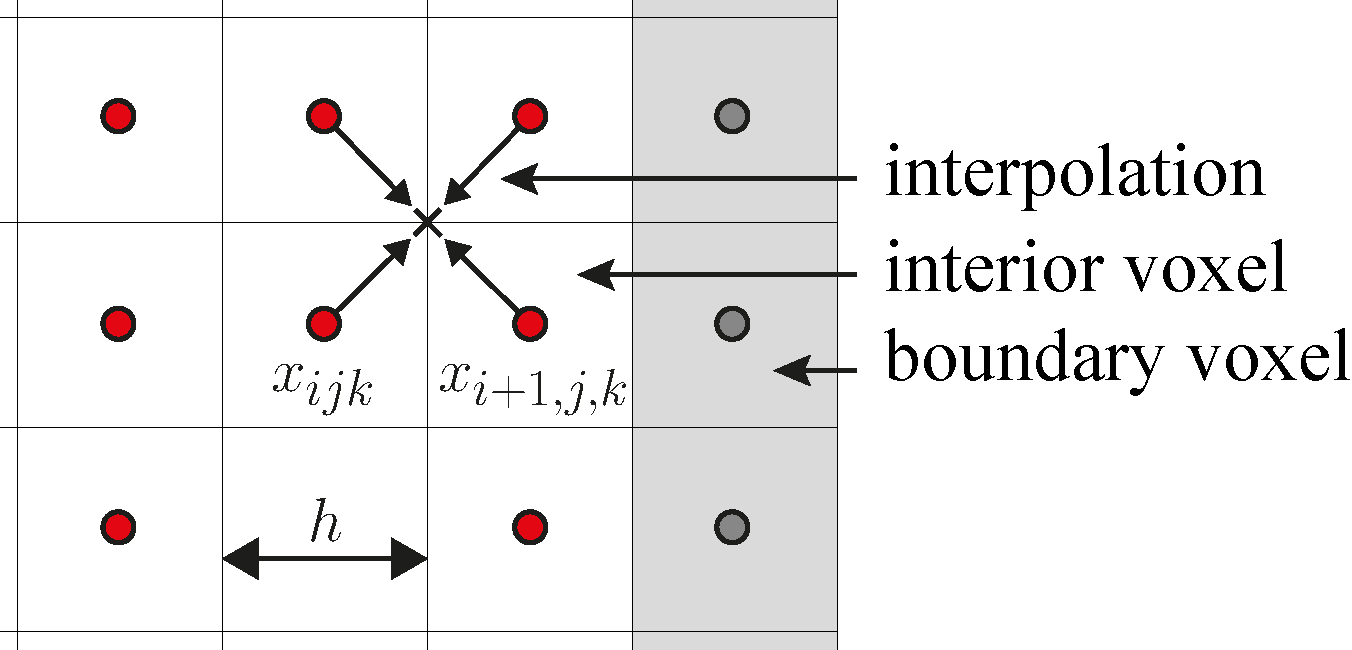
\includegraphics[width=0.6\textwidth]{04_pn_method/figures/fig_fd_grids.pdf}
\caption{Image of finite difference grid showing domain (white cells), boundary (gray cells), gridpoints (red), voxelsize $h$ and interpolation.}
\label{fig:pn_solver_finite_difference_grid}
\end{figure}

The first step during a discretization is the replacement of $\vec{x}$ by its discrete counterpart $x_{ijk}$. Using the two-dimensional Laplace equation $\nabla^2\phi(\vec{x})=q(\vec{x})$ as an example, this results in:
\begin{align*}
\nabla^2\phi\left(\vec{x}\right)=q\left(\vec{x}\right)
\xrightarrow{\vec{x} = x_{ijk}}
\partial_x^2\phi_{ij}+
\partial_y^2\phi_{ij}
=
q_{ij}
\end{align*}
For notational convenience $\phi_{ijk} = \phi\left(x_{ijk}\right)$ is defined. The spatial derivatives are approximated using central differences:
\begin{align}
\partial_x\phi_{ijk} = \frac{\phi_{i+\frac{1}{2}jk} - \phi_{i-\frac{1}{2}jk}}{h_x}
\label{eq:pn_solver_central_difference}
\end{align}
Continuing with the Laplace example, the substitutions of spatial derivatives are carried out next. Nested derivatives affect the indices accordingly:
\begin{align}
&
\xrightarrow{\text{central difference}}
\left(
\frac
{
\partial_x
\phi_{i+\frac{1}{2}j}
-
\partial_x
\phi_{i-\frac{1}{2}j}
}
{h_x}
\right)
-
\left(
\frac
{
\partial_y
\phi_{ij+\frac{1}{2}}
-
\partial_y
\phi_{ij-\frac{1}{2}}
}
{h_y}
\right)
=
q_{ij}
\nonumber
\\
&
\xrightarrow{\text{central difference}}
\frac
{
\frac{\phi_{i+1j} - \phi_{ij}}{h_x}
-
\frac{\phi_{ij} - \phi_{i-1j}}{h_x}
}
{h_x}
-
\frac
{
\frac{\phi_{ij+1} - \phi_{ij}}{h_y}
-
\frac{\phi_{ij} - \phi_{ij-1}}{h_y}
}
{h_y}
=
q_{ij}
\label{eq:laplace-central-difference}
\end{align}

\subsubsection*{Canonical Form}
After application of the discretization, equation \ref{eq:laplace-central-difference} is further brought into canonical form, which means that it is factorized according to the unknowns $\phi_{ij}$. This results in the discretized Laplace equation:
\begin{align}
\xrightarrow{\text{factorization}}
\frac{1}{h_x^2}\phi_{i+1j}
+\frac{1}{h_x^2}\phi_{i-1j}
+\frac{1}{h_y^2}\phi_{ij+1}
+\frac{1}{h_y^2}\phi_{ij-1}
-2\left(\frac{1}{h_x^2}+\frac{1}{h_y^2}\right)\phi_{ij}
=
q_{ij}
\label{eq:pn_laplace_canonical_form}
\end{align}

\subsubsection*{Stencil Code Crafting}

Consequently, the canonical form is used to derive the stencil code. This is done by interpreting the equation as a product between a row in the coefficient matrix $A$ and the vector of unknowns (the solution vector $\vec{u}$), resulting in the right hand side $q_{ij}$. The regular structure of the discretization reveals a pattern, which is the same for every row and is called a stencil code.

\begin{figure}[h]
\centering
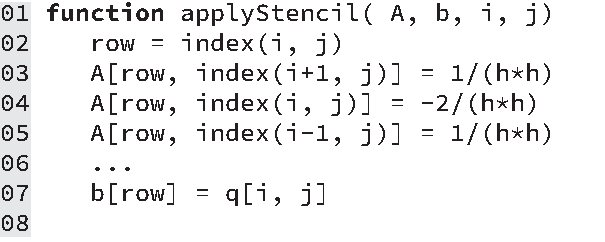
\includegraphics[width=0.6\textwidth]{04_pn_method/figures/fig_code_stencil.pdf}
%\missingfigure{source code figure for simple stencil code}
\caption{Spatial discretization of partial differential equations will lead to stencil code which is executed to populate the system matrix $A$ and right hand side vector $b$.}
\label{fig:pn_solver_stencil_code}
\end{figure}

The purpose of the stencil code is to be executed repeatedly to populate the system matrix $A$ and right hand side $\vec{b}$. This requires a mapping of multi-dimensional indices $ijk$ to linear indices into rows of $\vec{u}$ (and columns of $A$). This mapping is referred to as the \emph{index} function. The components of the solution vector $\vec{u}$ are associated with unknowns at specific grid locations $ijk$. In case of the Laplace example this would be written as:
\begin{align}
u_{\operatorname{index}\left(ijk\right)} = \phi_{ijk}\quad\text{ with }\quad \operatorname{index}: \mathbb{Z}^3\mapsto\mathbb{Z}
\label{eq:pn_index_mapping}
\end{align}

Also functions for accessing discretized input fields (such as $q$ in the Laplace example) and parameters, such as the voxel size $h$, will be called by the stencil code to retrieve required values.

\subsubsection*{System Matrix Population and Solve}
The stencil code is compiled once and then executed for each row in $A$ to populate the system. Different standard methods for solving the linear system $A\vec{u}=\vec{b}$ can be applied to find the solution $\vec{u}$, the discretized radiance field. This solution can then be used in a rendering application.
\begin{figure}[h]
\centering
%\missingfigure{image overview of the numerical pipeline}
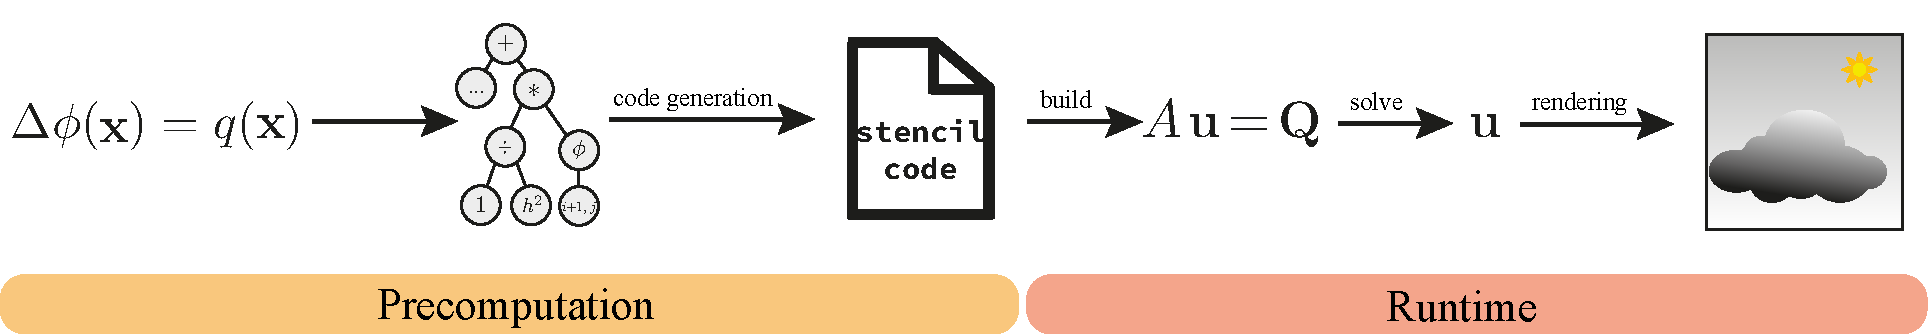
\includegraphics[width=1.0\textwidth]{04_pn_method/figures/fig_pipeline.pdf}
\caption{Overview of the method for solving the $P_N$-equations which is introduced in this chapter. The core idea is to automate the stencil code generation using a computer algebra representation of the equations.}
\label{fig:pn_solver_stencil_overview}
\end{figure}

In the following subsections, the new solver will be introduced as as a general framwork for automization of the steps for system building. The first subsection discusses how a computer algebra representation is used to represent the equation to be solved. Subsection~\ref{sec:pn_stencil_gen} shows how the spatial discretization and stencil code generation are modeled as operations on that representation. Subsection~\ref{sec:pn_bc} explains the aspects of the system that are related to boundary conditions, followed by subsection~\ref{sec:pn_framework} which discusses the surrounding framework and how the generated stencil is used within that framework. Subsection~\ref{sec:pn_staggered} elaborates on the extension of the solver to staggered grids, which is necessary for the solver to produce useful results. Finally, subsection~\ref{sec:pn_system_matrix} is dedicated to properties of the coefficient matrix $A$ and methods for solving the linear system.

\subsection{Computer Algebra Representation}
\label{sec:pn_car}

At the core of the solver is a computer algebra representation of the equations, which the system is trying to solve on a given domain. This representation is a mathematical expression tree (Preiss~\cite{Preiss00}). Each node within that tree can have any number of children and represents a constant, mathematical symbol or a mathematical operation, such as integration, derivation, power, addition or multiplication. Representations of complex equations are constructed by nesting nodes into a larger tree, where child nodes are considered as arguments of the operation, represented by the parent node.

A number of computer algebra systems exist, such as SymPy~\cite{Meurer17}, which allow to generate and manipulate computer algebra representations. However, for this thesis a small lightweight computer algebra representation containing the required subset has been developed. Figure~\ref{fig:pn_math_expression_tree_generation} demonstrates how this system is used to build the expression trees for the examples above.
\begin{figure}[h]
\centering
%\missingfigure{code listing showing how the expression tree is build}
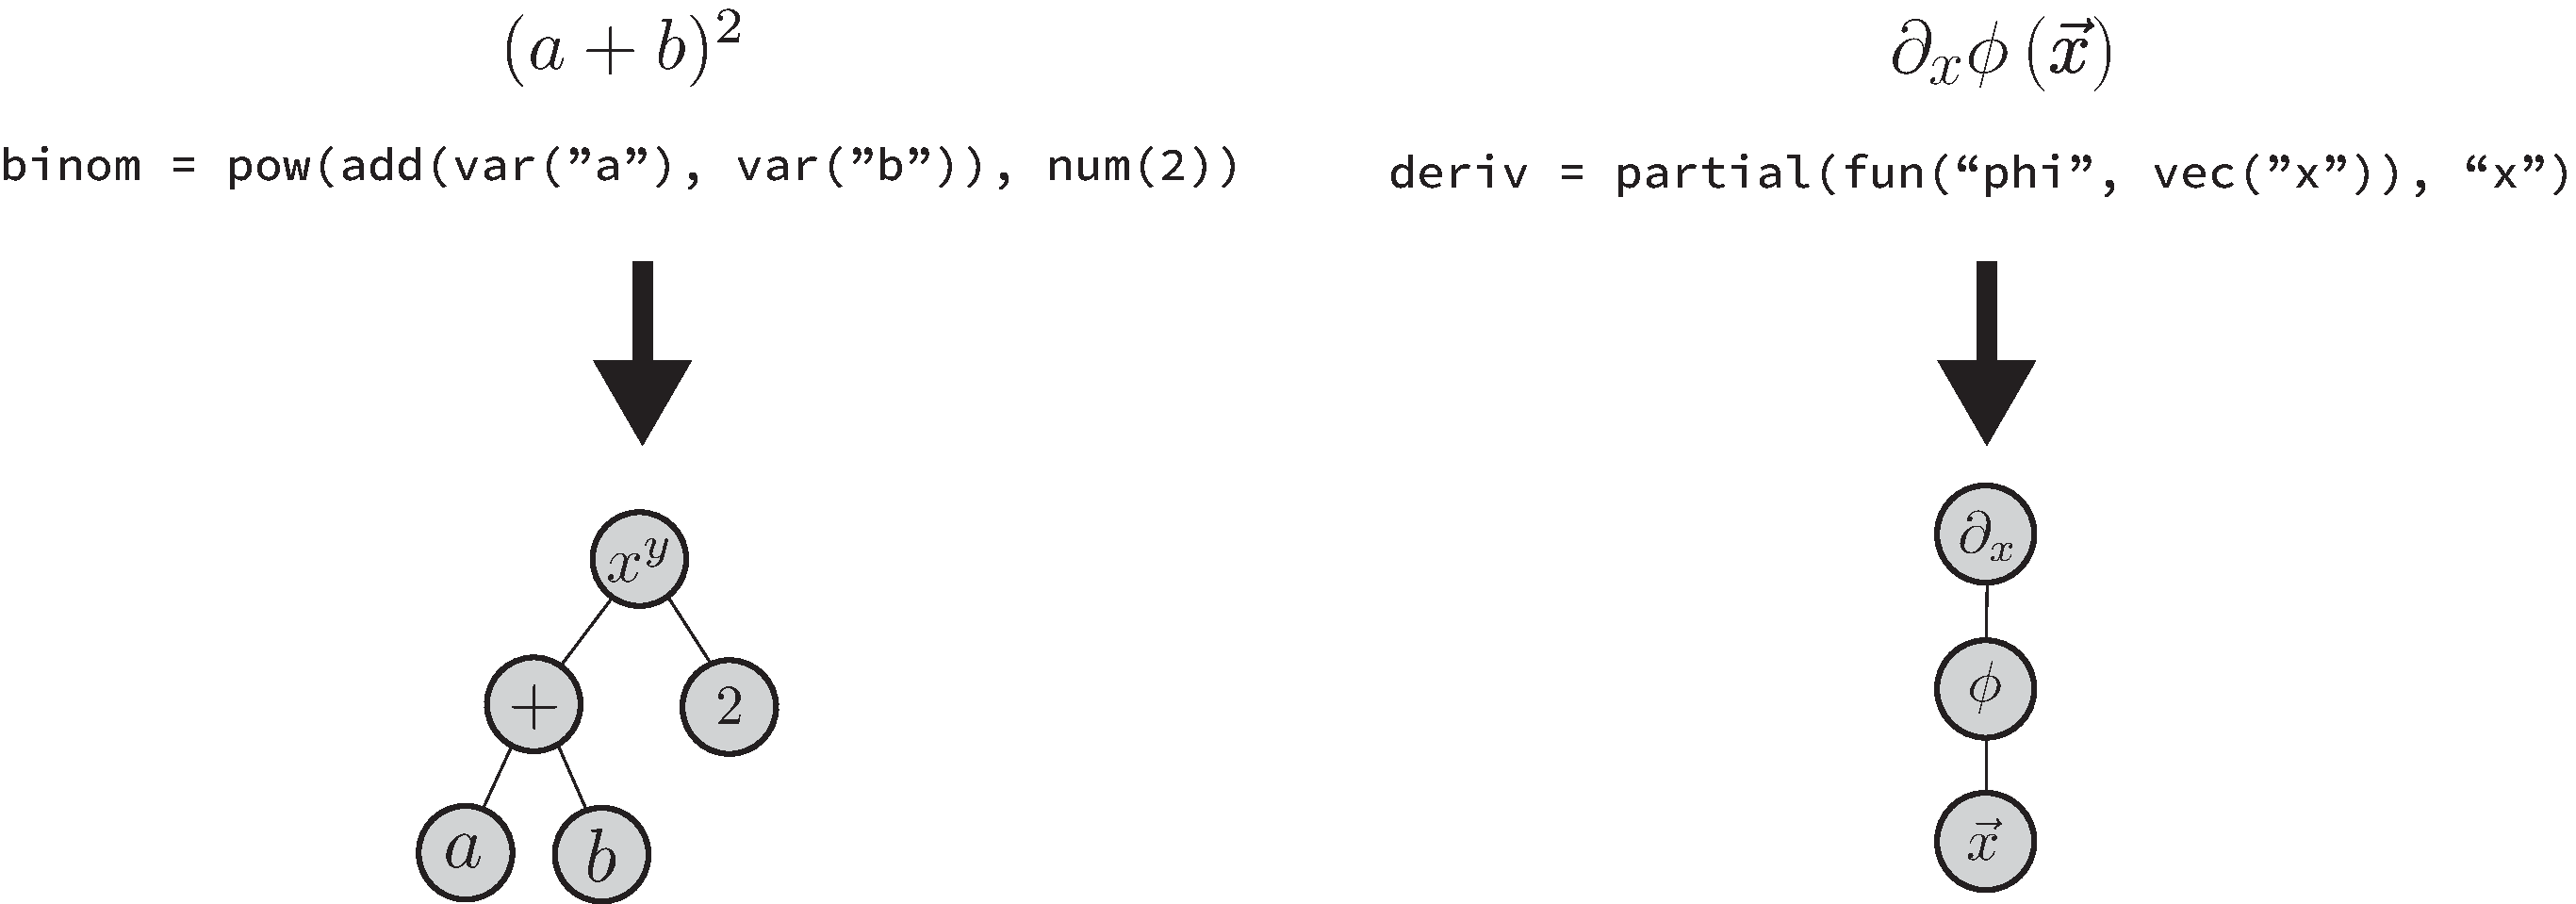
\includegraphics[width=1.0\textwidth]{04_pn_method/figures/fig_car_representation2.pdf}
\caption{An Python-API is used to create the expression tree representation for mathematical expressions.}
\label{fig:pn_math_expression_tree_generation}
\end{figure}

Manipulations of mathematical expressions, such as expansions, the application of identities, substitution, factorization or rearranging of terms can be expressed as operations on the expression tree (see figure~\ref{fig:pn_math_expression_tree_manipulation}). Section~\ref{sec:pn_stencil_gen} will assess how the spatial discretization is carried out as such an operation.
\begin{figure}[h]
\centering
%\missingfigure{image of representing binomial expansion as operation on expression tree}
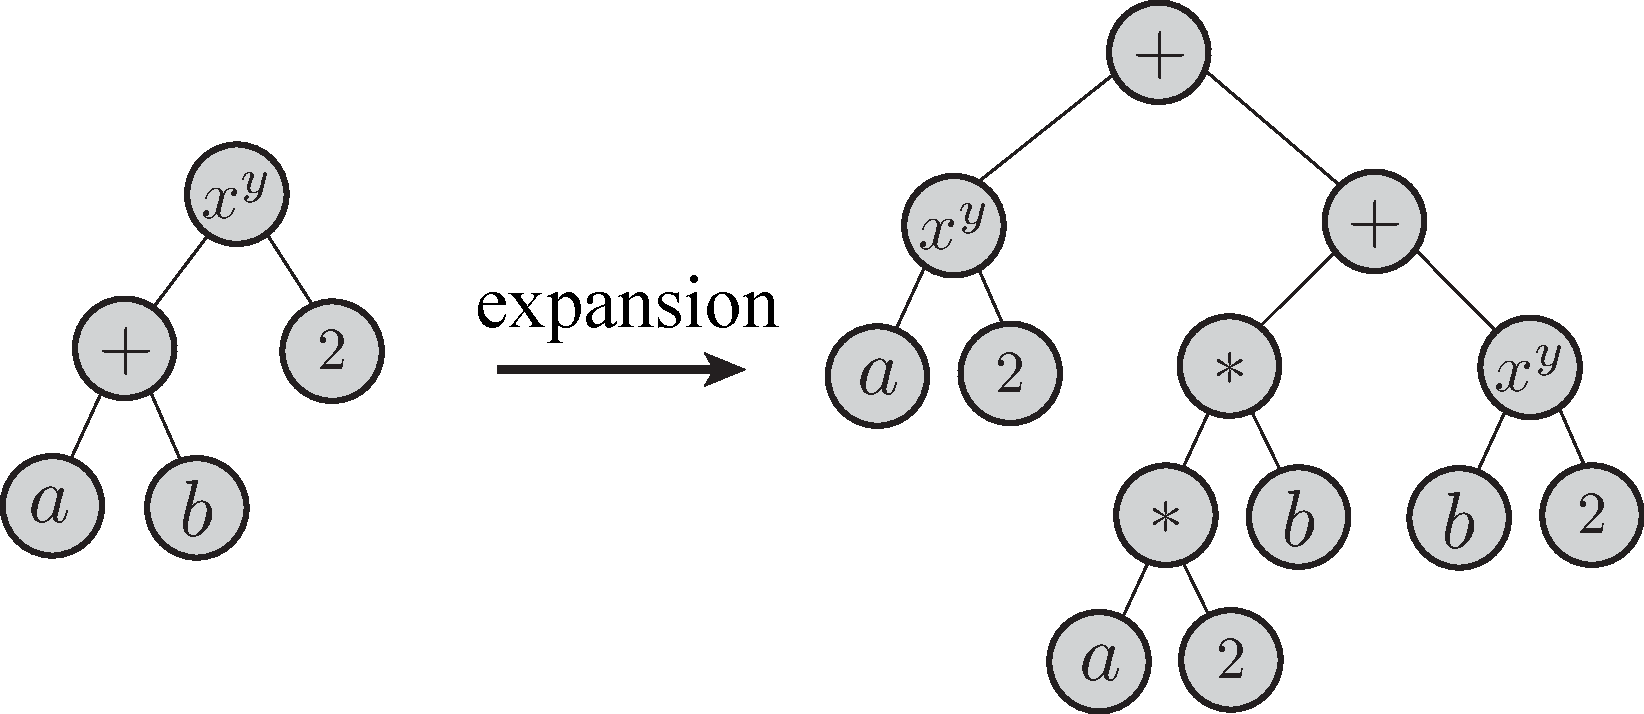
\includegraphics[width=0.7\textwidth]{04_pn_method/figures/fig_car_expansion.pdf}
\caption{Algebraic manipulations of equations are expressed as operations on the expression tree given by the computer algebra representation.}
\label{fig:pn_math_expression_tree_manipulation}
\end{figure}

\subsection{Discretization}
\label{sec:pn_stencil_gen}

After expressing the $P_N$-equations in the computer algebra representation, the spatial discretization is carried out as a manipulation step on the mathematical expression tree. This is done by parsing the tree from the root. The equation is supposed to be discretized at position $\vec{x}$, which initially coincides with the location $x_{ijk}$ in the discretized domain. This location is kept on a stack by the parser.

When a differential operator is encountered during tree parsing, the subtree representing the expression to be derived is instantiated twice according to the finite difference expression in equation~\ref{eq:pn_solver_central_difference} with appropriate weighting factors. The current position on the stack is adjusted and pushed on the stack again when descending down in the tree on each side of the central difference expression. This will produce higher order stencils for nested differential operators.
\begin{figure}[h]
\centering
%\missingfigure{image showing math expression tree for how the differential operator is being replaced with central difference. also mark the position on the stack.}
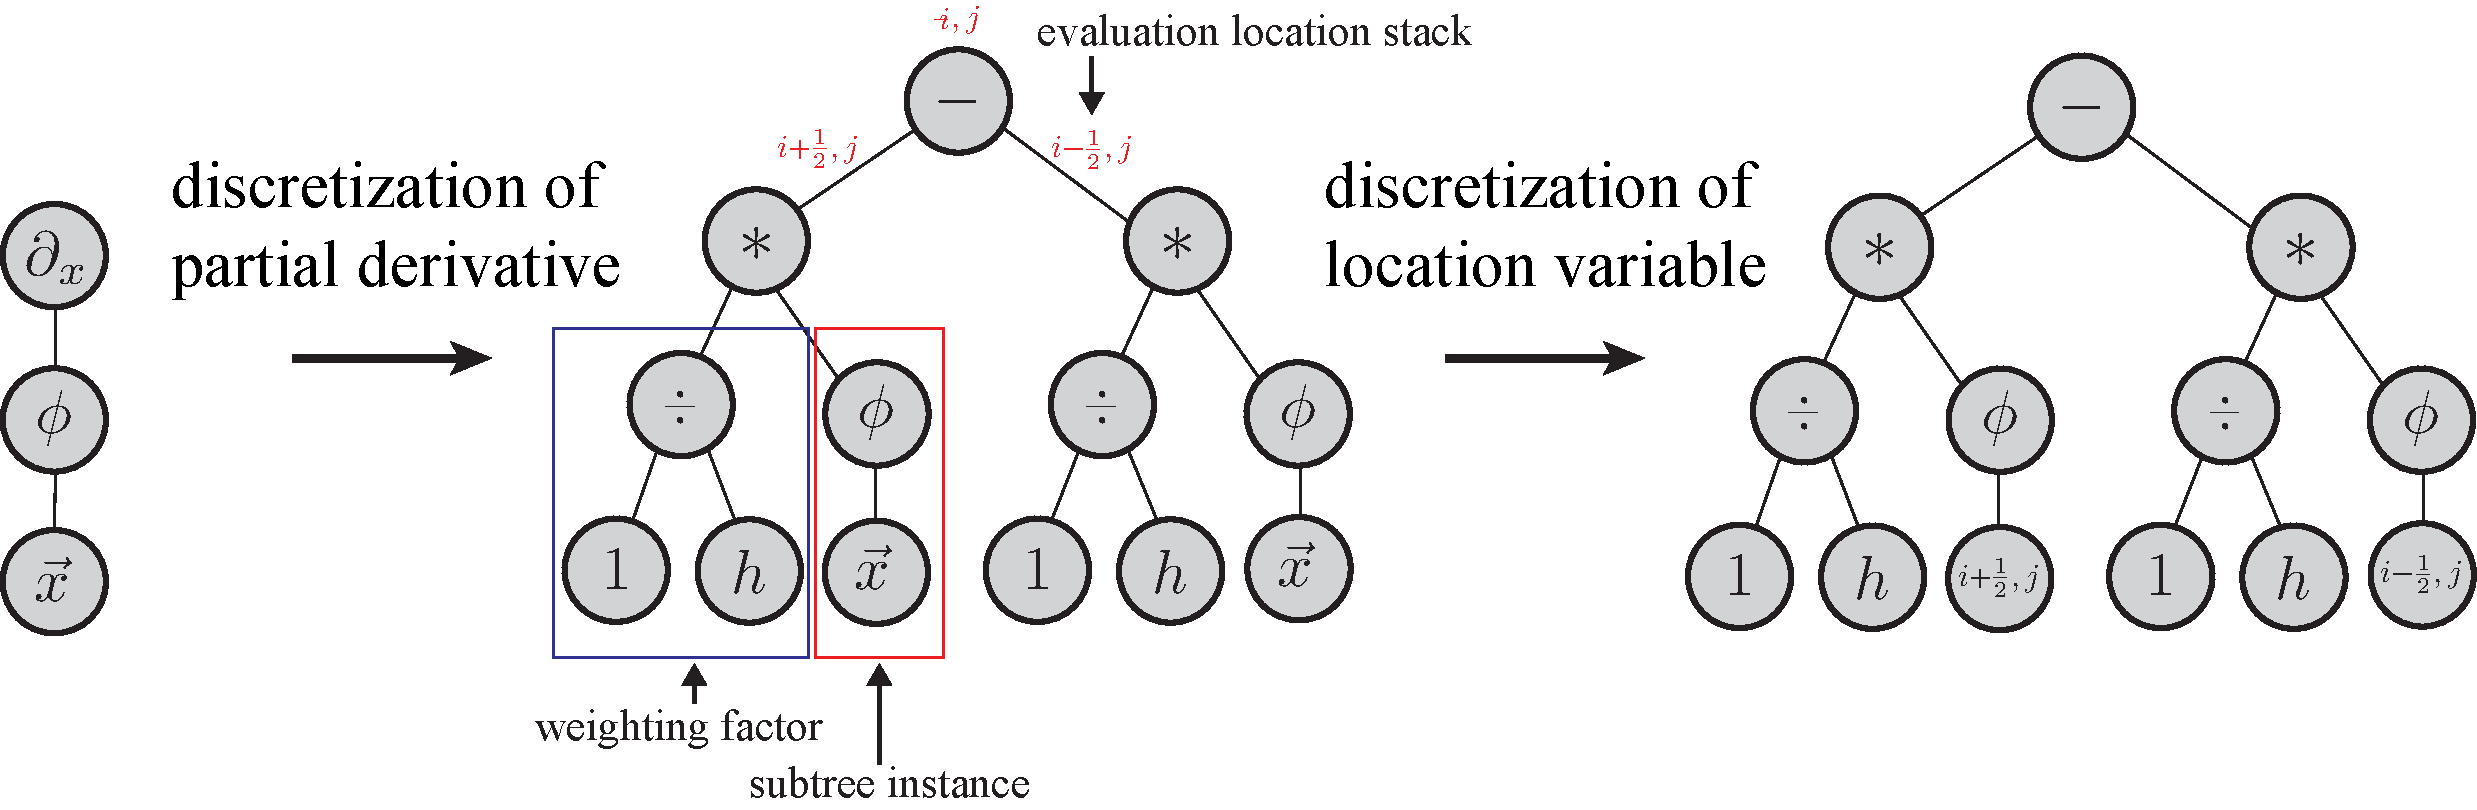
\includegraphics[width=1.0\textwidth]{04_pn_method/figures/fig_car_discretization.pdf}
\caption{Discretization is carried out as an operation on the expression tree where partial derivatives are replaced by finite difference subtrees. Continous variables are replaced by discrete counterparts, for which offsets are retrieved from a stack that is maintained during tree parsing.}
\label{fig:pn_discretization_differential}
\end{figure}

Once the parser arrives at the symbol $\vec{x}$ in the tree, it is replaced by its discrete counterpart. The top of the discrete position stack indicates where the unknown is expected to be evaluated relative to position $ijk$, at which the whole equation is being evaluated. If the position on top of the stack is the same, then the unknown at $ijk$ is used to replace $\vec{x}$ in the expression. If the unknown is expected to be evaluated at a different location than $ijk$ (due to central differences), then $\vec{x}$ is being substituted by an expression which expresses the interpolation of the unknowns from the gridpoints at which they are defined for the position on top of the stack (figure~\ref{fig:pn_discretization_interpolation}). This ensures, that the final expression only contains unknowns, for which an element in the solution vector exists. This will automatically handle the introduction of staggered grids later in section~\ref{sec:pn_staggered}.
\begin{figure}[h]
\centering
%\missingfigure{image showing interpolation.}
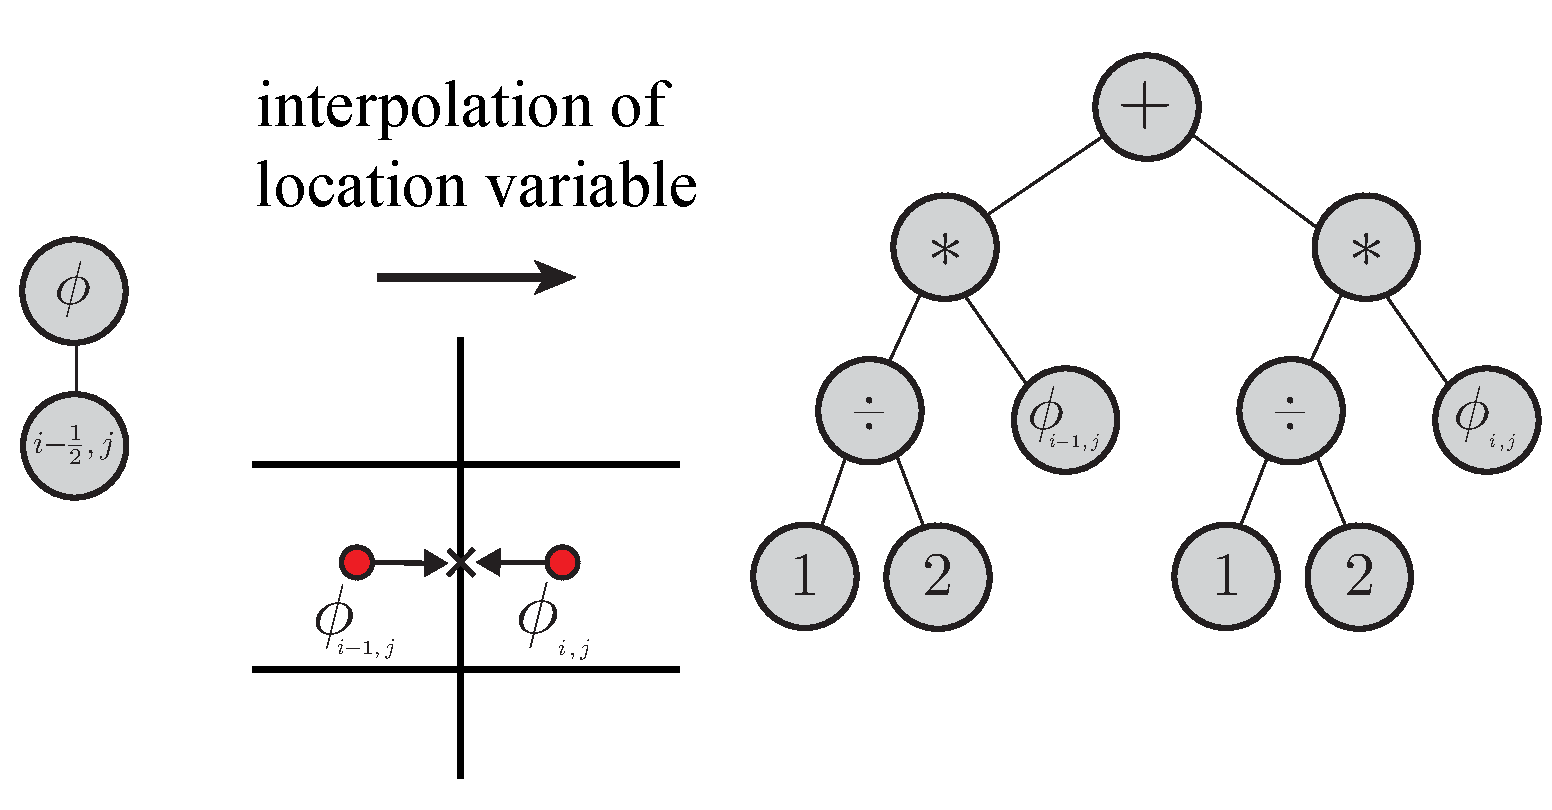
\includegraphics[width=0.7\textwidth]{04_pn_method/figures/fig_car_interpolation.pdf}
\caption{Continuous field variables are turned into discrete counterparts by replacing them with an expression subtree which realizes an interpolation.}
\label{fig:pn_discretization_interpolation}
\end{figure}

After applying the discretization to the expression tree, the equation is being factorized according to the unknowns ($\phi$ in the Laplace example). The factorization is applied as a sequence of manipulation operations to the expression tree, including application of the distributive law. A seperate step iterates over all resulting terms and merges coefficients from multiple instances of the same unknown, so that each unknown appears only once (canonical form).

\subsection{Stencil Code Generation}
\label{sec:pn_stencil_gen2}

The expression tree of the canoncial form is analyzed and rendered into stencil code. This is facilitated by different rendering frontends which allow for rendering the expression tree to latex or C++-code (see figure~\ref{fig:pn_math_expression_tree_rendering}).
\begin{figure}[h]
\centering
%\missingfigure{image showing rendering frontends for source code and latex}
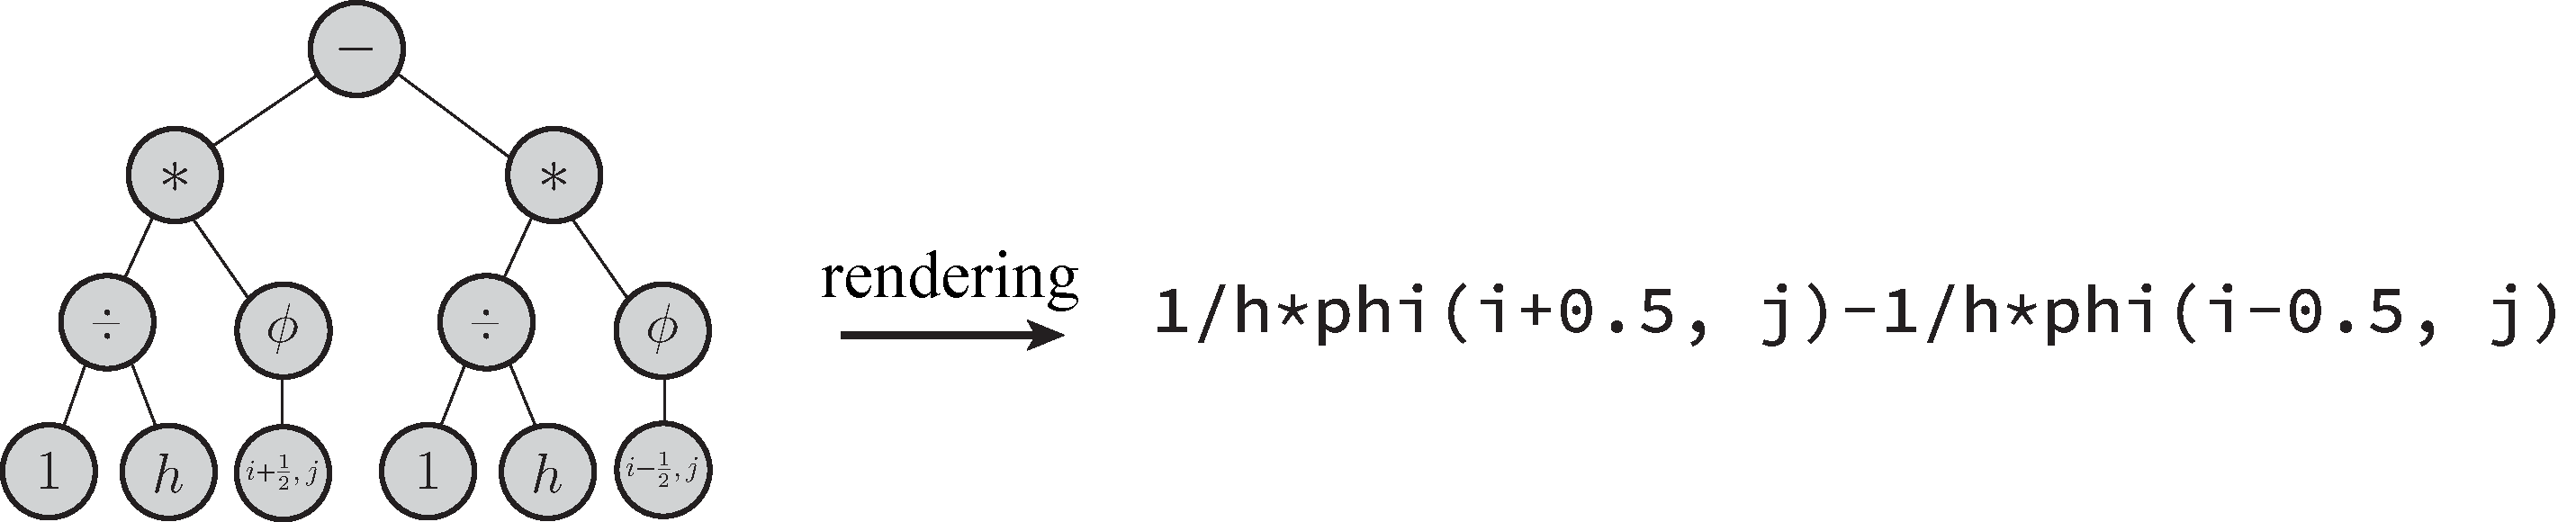
\includegraphics[width=1.0\textwidth]{04_pn_method/figures/fig_car_rendering.pdf}
\caption{Rendering frontends allow turning expression trees into source code.}
\label{fig:pn_math_expression_tree_rendering}
\end{figure}

If a term contains an unknown, then its factor expression subtree is rendered into a source code string. The symbols for voxel size and other radiative quantities are replaced by function calls into an API, which is being provided by the framework. Finally, the voxel-space coordinate associated with the unknown is used to find a discrete index into the finite difference grid, relative to the original coordinate $ijk$, at which the equation is being evaluated. This discrete index is being used to compute the column in $A$. Hence the assignment expression in the stencil code can be put together.
\begin{figure}[h]
\centering
%\missingfigure{image showing code generation from expression tree in canonical form.}
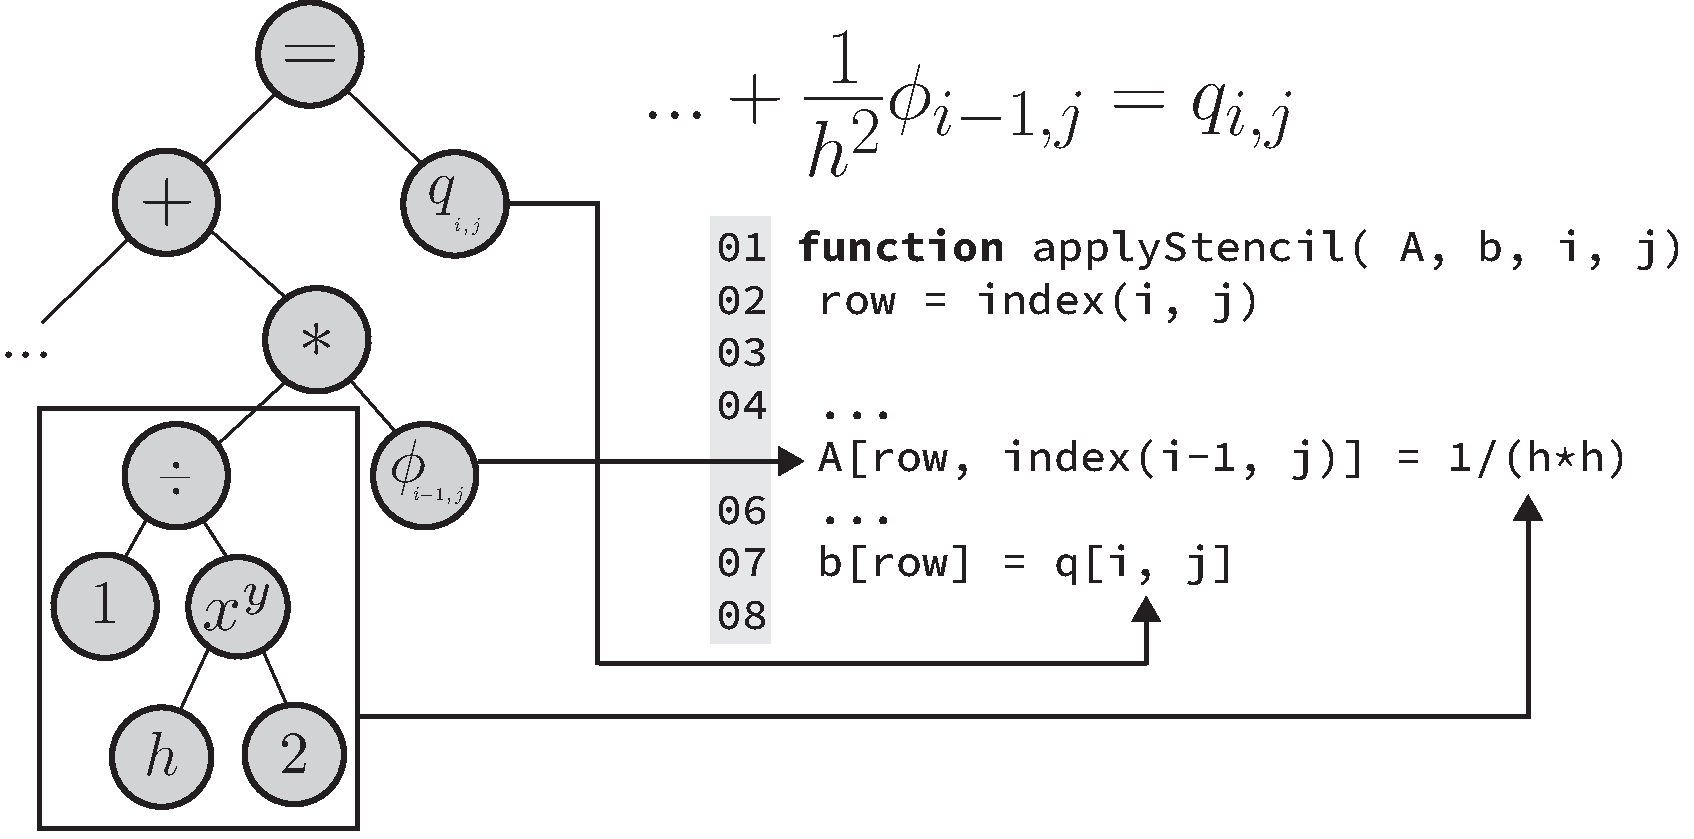
\includegraphics[width=0.6\textwidth]{04_pn_method/figures/fig_car_canonical_to_code.pdf}
\caption{The discretized equation in canonical form allows straightforward generation of stencil code from the different parts of the expression tree.}
\label{fig:pn_discretization_codegen}
\end{figure}

If the term does not contain an unknown, the whole term is rendered into a single expression, which is being assigned to the current row of the right hand side vector $\vec{b}$.

The stencil code is generated with the assumption of certain function calls being available. These are integrated into a single API which is being provided by the solver framework (figure~\ref{fig:pn_discretization_codegen_stencilAPI}). This API allows the stencil to query the current row in the system for which it is being executed, the voxelsize as well as functions for accessing discrete radiative transfer properties.
\begin{figure}[h]
\centering
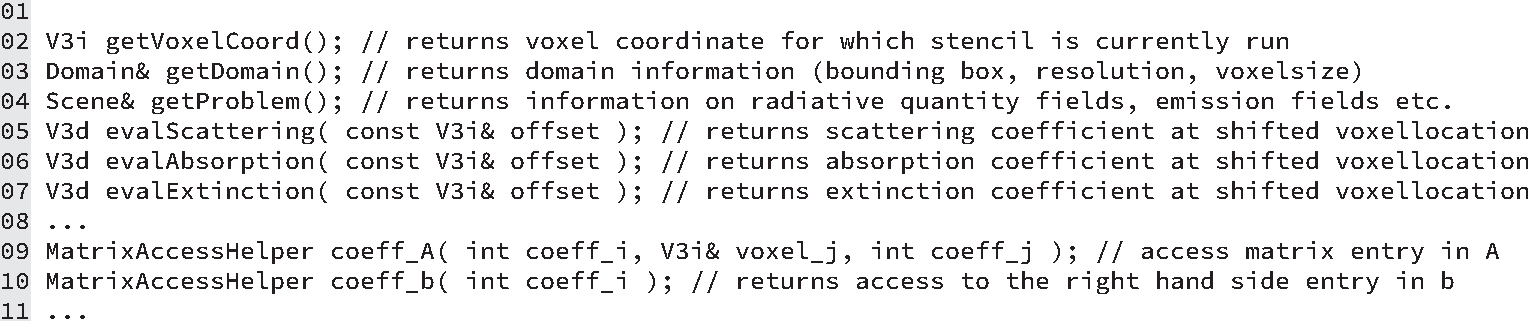
\includegraphics[width=0.95\textwidth]{04_pn_method/figures/fig_stencil_api.pdf}
%\missingfigure{image showing the stencil API}
\caption{Stencil code generation assumes an API for querying voxel fields of radiative quantities and accessing entries in coefficient matrix $A$ and right hand side $b$}
\label{fig:pn_discretization_codegen_stencilAPI}
\end{figure}


\subsection{Boundary Conditions}
\label{sec:pn_bc}

Central difference discretization will introduce references to spherical harmonics coefficients, which are outside the computational domain. Those references will be part of the stencil code, which has been generated without the notion of boundaries and boundary conditions and are handled transparently by the solver framework.

Boundary conditions define how the problem behaves directly on the boundary interface of the domain, and are an important aspect of establishing the system of linear equations. Boundary conditions can be specified without effort through the Dirichlet boundary conditions and Neumann boundary conditions, which are both supported by the system introduced in this chapter.

If $D\in\mathbb{R}^3$ defines the volume of the computational domain across which to find a solution to a partial differential equation, then $\partial D\in\mathbb{R}^3$ can be the set of points, which lie directly on the boundary of that domain. With Dirichlet boundary conditions, the value of the unknown is specified at the interface $\partial D$ directly. With Neumann boundary conditions, the behavior of the solution at the boundary is specified by giving a normal derivative of the solution. Using the Laplace example, this would be:
\begin{align*}
\text{PDE:\ \ } & \nabla^2\phi\left(\vec{x}\right) = q\left(\vec{x}\right)
&
\\
\\
\text{Dirichlet BC:\ \ } & \phi\left(\vec{x}\right) = f\left(\vec{x}\right)
&\forall \vec{x}\in\partial D
\\
\\
\text{Neumann BC:\ \ } & \frac{\partial\phi\left(\vec{x}\right)}{\partial\vec{n}} = g\left(\vec{x}\right)
&\forall \vec{x}\in\partial D
\end{align*}
In most applications for computer graphics, a value of zero for either Dirichlet or Neumann boundaries is adequate and is handled by the system through remapping the index: Considering the first term of the discretized Laplace equation in equation~\ref{eq:pn_laplace_canonical_form}, the result is the following assignment within the stencil code:
\begin{align}
A[\mathrm{index}(i,j), \mathrm{index}(i+1, j)] = 1.0/(h_x*h_x);
\end{align}
The function call $index(i+1, j)$ will not be able to produce a valid column index into the coefficient matrix $A$ for voxels adjacent to the boundary, because the unknown $\phi$ has no discrete element in the solution vector voxels outside the domain. If the value of $\phi$ on the boundary is zero, then the unknown on the boundary voxel would be zero and its coefficient would not matter. Therefore, the simplest solution is to ignore the coefficient not writing anything into the matrix $A$. This equates to matrix $A$ being zero outside the computation domain.

In the solver framework, this is implemented by overloading the assignment operator. If the target coefficient of the assignment belongs to a boundary voxel and Dirichlet boundary conditions are enabled, then the assignment is simply ignored and no change to the system matrix $A$ is done.

\begin{figure}[h]
\centering
%\missingfigure{image: boundary voxels and dirichlet boundary condition. location of the boundary interface.maybe an arrow indicating the access of the stencil.show assignment and arrow to boundary voxel coefficient. then arrow to nil.also visualize the boundary surface.}
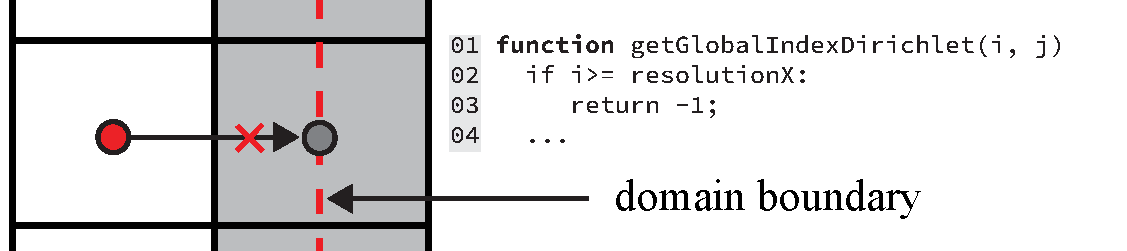
\includegraphics[width=0.8\textwidth]{04_pn_method/figures/fig_bc_dirichlet.pdf}
\caption{Dirichlet boundary conditions with zero value are modelled by ignoring coefficient assignments to boundary voxels.}
\label{fig:pn_bc_dirichlet}
\end{figure}

With Neumann boundary conditions, the derivative is specified at the boundary. Since the derivative is found using central differences between two adjacent voxels, the boundary condition is controlled by how the coefficient at the voxel near the boundary relates to its adjacent coefficient at the boundary voxel. In the simplest case, the derivative is set to zero, in which the boundary voxel coefficient needs to be identical with its adjacent voxel inside
\begin{align*}
\partial\phi=0\quad\forall\phi\in\partial D
\implies
\frac{\phi_{i+1,j}-\phi_{i,j}}{h_x} = 0
\implies
\phi_{i+1,j}=\phi_{i,j}
\ .
\end{align*}
In the case of adjacent coefficients being equal across the boundary interface, a coefficient $b$ assigned to the boundary $\phi_{i+1,j}$ can be added to the adjacent unknown inside the domain resulting in:
\begin{align}
a\phi_{i,j} + b\phi_{i+1,j} = \left(a+b\right)\phi_{i,j}
\quad \text{with}\quad \phi_{i+1,j}=\phi_{i,j}
\end{align}

In the solver framework, this is implemented by index remapping. If the target coefficient of the assignment belongs to a boundary voxel and Neumann boundary conditions are enabled, then the index function returns the index of the adjacent voxel inside the domain.

\begin{figure}[h]
\centering
%\missingfigure{image showing neumann boundary conditions and index bending. also visualize the boundary surface.}
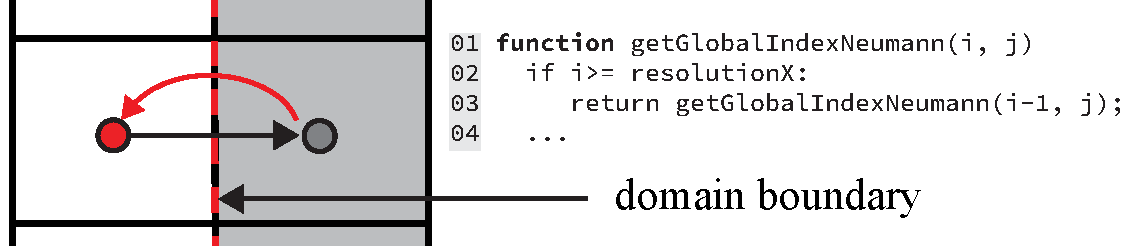
\includegraphics[width=0.8\textwidth]{04_pn_method/figures/fig_bc_neumann.pdf}
\caption{Neumann boundary conditions with zero value are modelled by remapping indices towards the adjacent inner voxel when assigning coefficients.}
\label{fig:pn_bc_neumann}
\end{figure}

Note how the choice and implementation of the boundary condition has an effect on where the effective boundary interface of the domain is located. With Dirichlet boundary conditions, the interface is directly located at the voxel centers of boundary voxels, while with Neumann boundary conditions, the interface is located at directly between the boundary voxels and inner voxels (figure~\ref{fig:pn_bc_dirichlet} and figure~\ref{fig:pn_bc_neumann}).

\subsection{Solver Framework}
\label{sec:pn_framework}

The stencil code is the result of the automated discretization step, which is carried out on the computer algebra representation and rendered into source code. The resulting stencil code is compiled and linked with a solver framework, which runs it to propagate the system matrix $A$ and right hand side vector $\vec{b}$. By rendering the tree to a different representation and assuming a different API used by the stencil code, different solver frameworks can be supported.
Therefore, the details about the surrounding framework are not relevant to the method in this thesis. In this section, however, an outline of the framework, which was implemented as part of this thesis will be given.
\begin{figure}[h]
\centering
%\missingfigure{class diagram of solver framework, including stencil, stencil api, voxelmanager, fields and pnsystem}
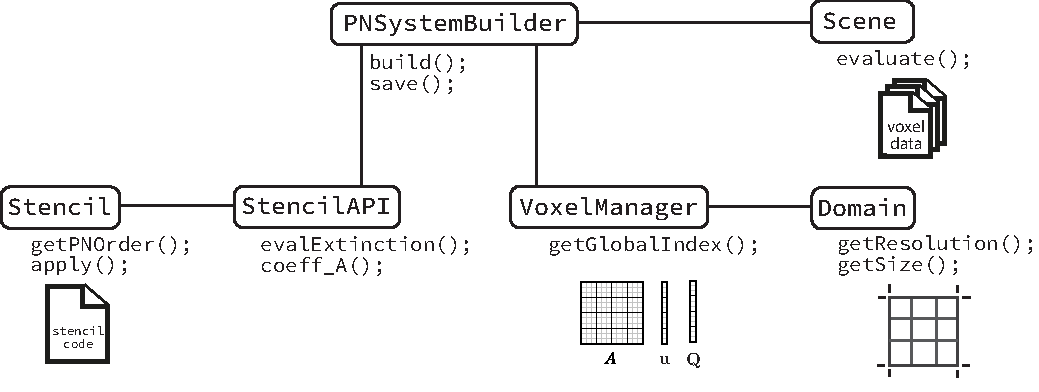
\includegraphics[width=0.95\textwidth]{04_pn_method/figures/fig_pn_solver_architecture.pdf}
\caption{High level overview over the $P_N$-solver architecture.}
\label{fig:pn_classes}
\end{figure}

The \emph{Stencil} class is the key structure around which the system is designed, and which serves as a wrapper around the generated stencil code. It specifies the dimension (two- or threedimensional) and the truncation order $N$, as these parameters are being decided during stencil code generation. The \emph{Stencil} class also indirectly specifies the number of spherical harmonics coefficients per voxel. It further specifies the placement of each spherical harmonics coefficient within the voxel. This will become important when staggered grids are introduced. The stencil specifies the highest order of any derivative operator, which was found during discretization. This affects the number of layers of boundary voxels around the computational domain. Finally, the \emph{Stencil} class has an apply function, which takes the reference to a \emph{StencilAPI} object as an input and runs the generated stencil code that uses that API to propagate the system matrix $A$ and right hand side vector $\vec{b}$.

The \emph{StencilAPI} class serves as the single interface between the generated stencil code and the surrounding parts of the framework. Figure~\ref{fig:pn_discretization_codegen_stencilAPI} gives an overview of the different query functions offered by the API. Essential are functions for mapping between coordinate spaces, such as world-space, voxel-space, discrete grid coordinates $ijk$ and linear indices into the solution vector. Further, those functions allow querying radiative transfer quantities, such as extinction coefficient or phase function spherical harmonics coefficients at world space positions. Both groups of functions will make use of a reference to a \emph{VoxelManager} and a \emph{Scene} class, respectively.

The \emph{Scene} class contains all inputs required to specify the problem to be solved. A \emph{Domain} object describes the extent of the computational domain in world-space, as well as the resolution of the finite difference grid. Further attached are references to abstract \emph{Field} interfaces, which allow querying scalar or vector fields at arbitrary worldspace positions for extinction coefficient, albedo, and the spherical harmonics coefficients of phase function and emission field. This is the place where the problem description is provided as input to the system. Different implementations of these abstract interfaces can be used, such as \emph{Constant} fields or \emph{VoxelGrid} fields. This follows the idea of resolution independent volumes introduced by Tessendorf et al.~\cite{Tessendorf11}.

The resolution of the finite difference grid provided by the \emph{Domain} class and the number of spherical harmonics coefficients by the \emph{Stencil} class, impose the layout of the voxel grid on the system. The \emph{Stencil} class gives the highest order of the derivation operator found during discretization, and with that drives the number of layers of boundary voxels. The final system of linear equations has to be a single column solution vector with a coefficient matrix of compatible dimensions. Since the computational domain is discretized using grid coordinates $ijk$, a mapping from three-dimensional coordinates $ijk$ and spherical harmonics coefficient index $c$ to a linear global index needs to be provided. This task becomes more involved, when staggered grids are introduced. This bookkeeping of interior and boundary voxels and their contained spherical harmonics coefficients is performed by the \emph{VoxelManager} class. This class is initialized with the information about the grid resolution by the \emph{Domain}, number of boundary voxel layers, number of coefficients, and the position of each coefficient on the grid by the \emph{Stencil} class. It manages the memory and mapping from multidimensional grid indices to linear indices within the global system.

Finally, the \emph{PNSystemBuilder} class is the structure, which brings the different parts together. It is initialized wit the \emph{Scene} class and the \emph{Stencil} class. Both are provided by the client code and are used during initialization to set up the \emph{VoxelManager}, which provides the layout and setup for the solution vector $\vec{u}$, right hand side vector $\vec{b}$ and system matrix $A$. The purpose of the \emph{PNSystemBuilder} class is to build the system matrix $A$ and right hand side vector $\vec{b}$ and return both to client code. This is done by calling the \emph{build} function on the object.

The \emph{build} function iterates over all voxels. For each voxel, the \emph{StencilAPI} object is set up with the correct indices and data pointers and passed as an argument to a call of the \emph{apply} function of the \emph{Stencil} class. As explained in section~\ref{sec:pn_stencil_gen}, the stencil code will make appropriate calls to the \emph{StencilAPI} object, which will propagate the system matrix $A$ and right hand side vector $\vec{b}$ with the correct values for the row, corresponding to the current voxel in the cycle of the \emph{build} function. The system is fully propagated after the stencil has been executed for every voxel. Separate functions of the \emph{PNSystemBuilder} class allow querying the system matrix $A$ and right hand side vector $\vec{b}$ after those have been build.

\subsection{Staggered Grids}
\label{sec:pn_staggered}

In figure~\ref{fig:pn_staggered_grid_problems}\subref{fig:pn_collocated_grid_artefacts}, preliminary results for the two-dimensional checkerboard problem are shown, a popular reference problem for deterministic methods (section~\ref{sec:pn_results}). As seen in the figure, it suffers from severe artifacts, showing an oscillating structure. The cause for these artifacts is a known problem for partial differential equations, which have different quantities influencing each other at the same spatial grid locations. The problem is visualized in figure~\ref{fig:pn_staggered_grid_problems}\subref{fig:pn_staggered_grid_idea}, using a simple one-dimensional grid as an example. Shown is a simple setup with two variables, which are located at the same grid points, referred to as collocated grids. The variable $\beta$ depends on the derivative of $\alpha$. Due to central difference discretization, two different solutions that are decoupled from each other can emerge. These solutions are interleaved in an oscillating pattern throughout the grid as shown in the upper part of the figure.

\begin{figure}[h]
\centering
\begin{subfigure}[t]{0.49\columnwidth}
\centering
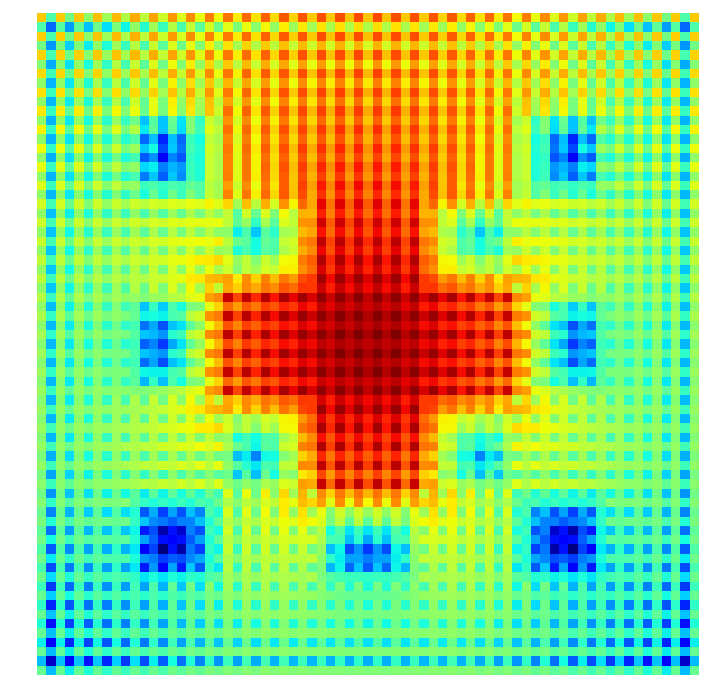
\includegraphics[width=\columnwidth]{04_pn_method/results/checkerboard2d_p1_collocated.png}
%\missingfigure{2d collocated solution with artefacts}
\caption{$P_1$-solution of the checkerboard problem using collocated discretization grid.}
\label{fig:pn_collocated_grid_artefacts}
\end{subfigure}%
\hspace{0.01\columnwidth}
\begin{subfigure}[t]{0.49\columnwidth}
\centering
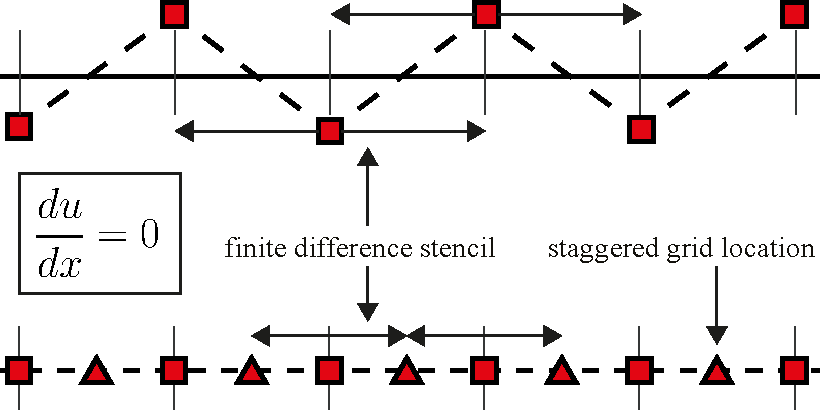
\includegraphics[width=\columnwidth]{04_pn_method/figures/fig_staggered_grid_1d_example.pdf}
%\missingfigure{1d schematic view of staggered grid idea, showing the problem with collocated grids}
\caption{Example showing the problem with finite differences producing a false solution (top) and its treatment with staggering (bottom).}
\label{fig:pn_staggered_grid_idea}
\end{subfigure}%
%\vspace{-0.2in}
\caption{Artefacts in the solution (left) due to shortcomings of collocated grid locations. These are addressed using staggered grids (exemplified right).}
\label{fig:pn_staggered_grid_problems}
\end{figure}

The solution to this problem is to offset the coefficients $\alpha$ and $\beta$ from each other spatially. This configuration is called staggered grids. As visualized in figure~\ref{fig:pn_staggered_grid_problems}\subref{fig:pn_staggered_grid_idea} bottom, setting up the coefficients in that way prevents decoupling and results in a single coherent solution throughout the grid. A similar staggering of the interdependent variables is required for the $P_N$-solver to produce correct results.

The staggered grid locations are found by subdividing the original grid into a finer grid of double resolution. The locations are at the grid points of that finer grid. In terms of the original grid, these are located at the voxel centers, the center of the voxel faces between adjacent voxels, the center of voxel edges and at voxel corners as shown in figure~\ref{fig:staggered_grid}.
\begin{figure}[h]
\centering
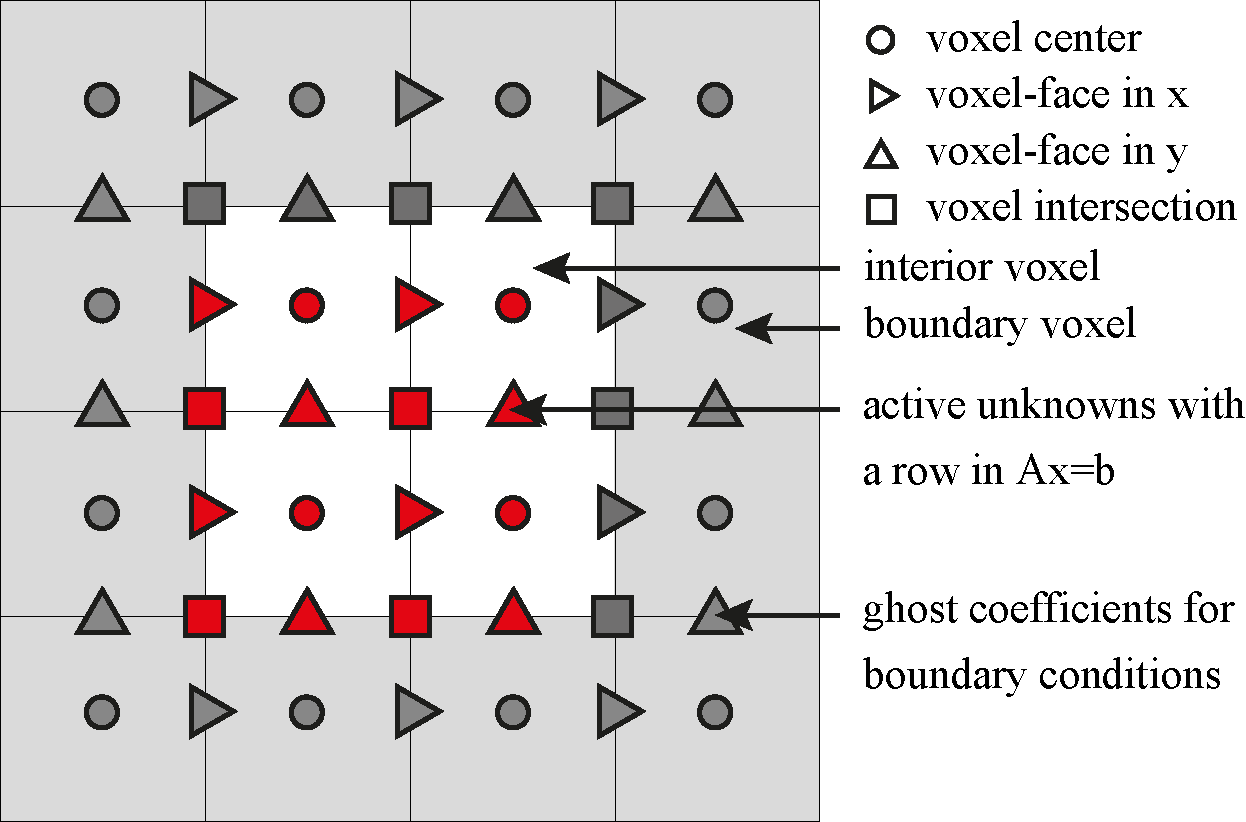
\includegraphics[width=0.65\textwidth]{04_pn_method/figures/fig_staggered_grid.pdf}
\caption{Staggered grid configuration in 2d. Extending the concept to 3d is straightforward.}
\label{fig:staggered_grid}
\end{figure}

With a staggered grid configuration, the question is which unknowns (the spherical harmonics coefficients) are placed at which staggered grid location. Seibold et al.~\cite{Seibold14} analysed the structure of the transport term and found that its discretization matrix relates coefficients to their derivatives in a very particular structure after converting the matrix to real-valued spherical harmonics. If coefficients are located on the staggered grid according to this structure, hence no interpolation is required when evaluating central differences of the stored coefficients (see figure~\ref{fig:staggered_grid_placement}).

Assuming this structure, the unknown locations are found by the following algorithm: First the zero coefficient is placed at the voxel center. Then all coefficients are found, which depend on derivatives of the zero coefficient. These coefficients are placed according to the central difference offsets. Following this, the coefficients are found, which depend on derivatives of the recently placed coefficients. The central difference offsets are used anew to find their new location. The particular structure of discretization matrix of the transport term in the real-valued $P_N$-equations is what allows placing the coefficients without any conflicts. 
\begin{figure}[h]
\centering
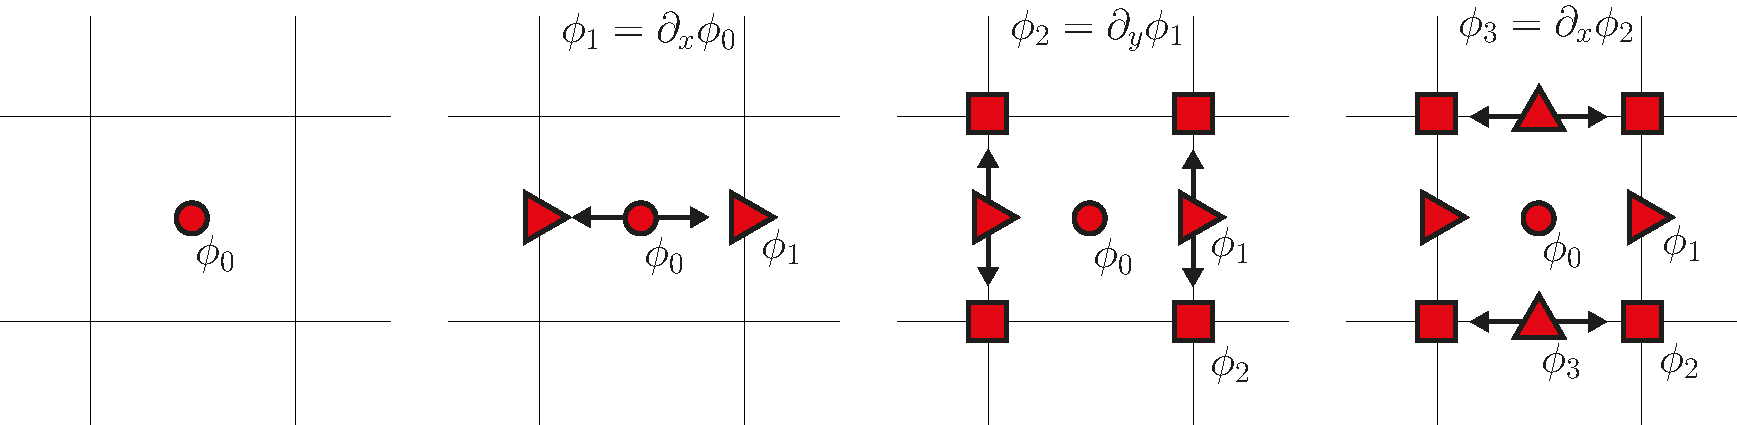
\includegraphics[width=0.95\textwidth]{04_pn_method/figures/fig_staggered_grid_finding_locations.pdf}
\caption{The process of finding staggered grid locations for unknowns $\phi_i$. The $P_N$-equations relate the unknowns through spatial derivatives, which imply an order on the finite difference grid. The first unknown is placed at the voxel center and the remaining unknown locations are found by following the spatial derivatives through the equations.}
\label{fig:staggered_grid_placement}
\end{figure}

It is important to realize that each equation in the system of linear equations relates a particular coefficient with spherical harmonics indices $l,m$ in a particular voxel within the finite difference grid to other coefficients at the same or adjacent voxels (due to derivatives). Therefore, the equation associated with a particular spherical harmonics index $l,m$ within the $P_N$-equations, is implicitly defined at the location of the spherical harmonics coefficient with the same $l,m$ index. Due to staggering, the equations are consequently defined at different locations. This has a paramount consequence for the spatial discretization step during stencil code generation.

In section~\ref{sec:pn_stencil_gen} the spatial discretization was carried out as a manipulation on the expression tree representing the $P_N$-equations. This manipulation step traversed the tree and replaced the continuous spatial variable $\vec{x}$ by its discrete counterpart $x_{ijk}$. During traversal, a stack was used to keep track of the current location which would change due to shifts from central difference discretizations of differential operators within the expression tree. This stack was initialized with the reference position $x_{ijk}$, which would refer to the voxel center. This was correct, as all coefficients and equations were collocated at this position. With staggered grids, the equations are to be evaluated at the grid location implied by the position of the respective spherical harmonics coefficient with index $l,m$. Therefore, to account for staggered grids, the position stack needs to be initialized with the staggered grid location of the $l,m$-equation, which is being discretized.

The discretization step will replace the evaluation of a coefficient at a particular location, with an interpolation of that coefficient from the surrounding grid locations at which it is defined (figure~\ref{fig:pn_discretization_interpolation}). This approach will handle the staggering naturally.

Staggering spherical harmonics coefficients also makes handling boundary conditions more involved. With collocated grids, it is straightforward to identify boundary voxels and voxels in the computational domain. Each voxel in the computational domain contributes the same number of unknowns to the system. With staggered grids, some boundary voxels will have a subset of their unknowns that lie directly on the boundary. Without changes to the system, this will imply a shifted boundary interface and introduce an asymmetry. Coefficients, which are located on the boundary, will be unknowns and part of the solution vector on one side and subject to boundary conditions on the other side (figure~\ref{fig:pn_staggered_grid_unhandled_bc}~\subref{fig:pn_staggering_asymmetry_bc}). This creates different boundary conditions on opposite sides of the problem domain and causes an asymmetry in the solution for symmetric problems (figure~\ref{fig:pn_staggered_grid_unhandled_bc}~\subref{fig:pn_staggering_asymmetry_bc_checkerboard}).
\begin{figure}[h]
\begin{subfigure}[t]{0.48\columnwidth}
\hspace{0.5in}
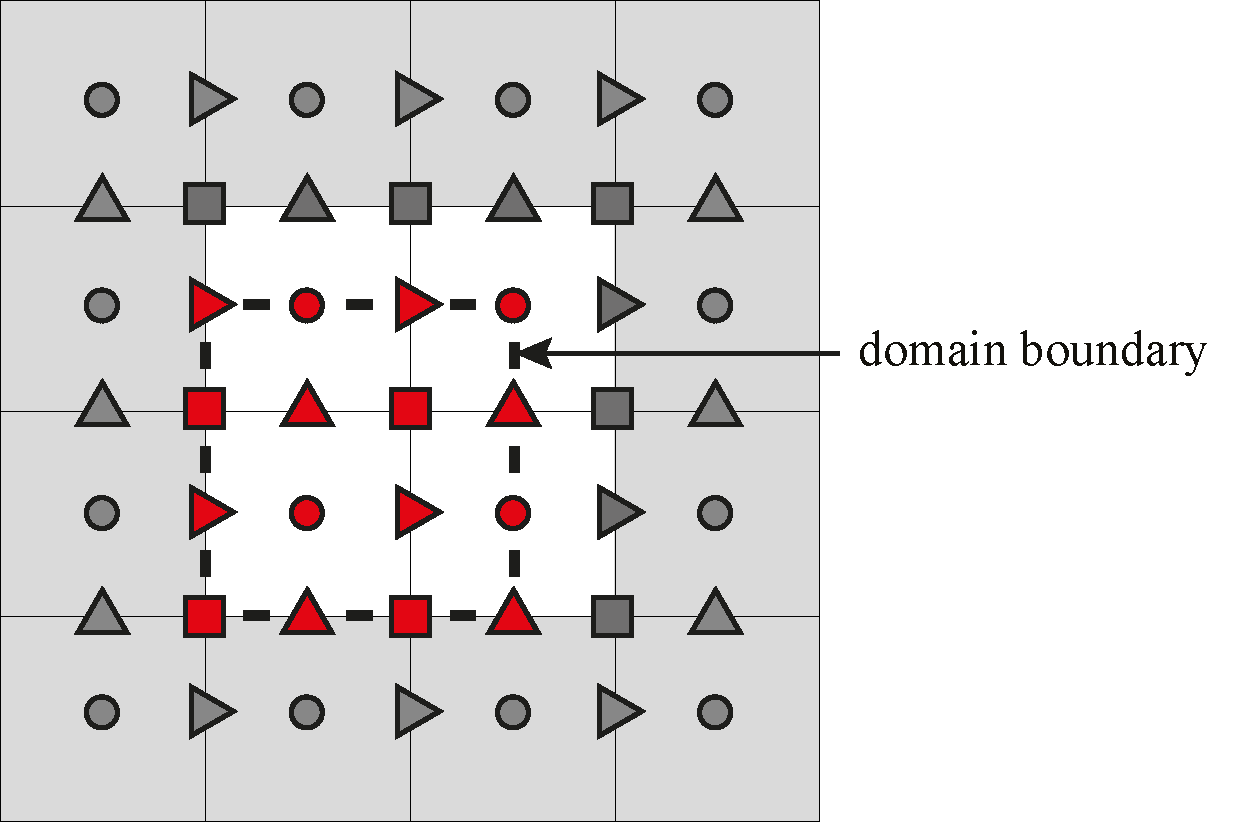
\includegraphics[width=1\textwidth]{04_pn_method/figures/fig_staggered_grid_domain_boundary_wrong.pdf}
\caption{Per voxel staggered grid locations.}
\label{fig:pn_staggering_asymmetry_bc}
\end{subfigure}
\hspace{0.01\columnwidth}
\begin{subfigure}[t]{0.48\columnwidth}
\centering
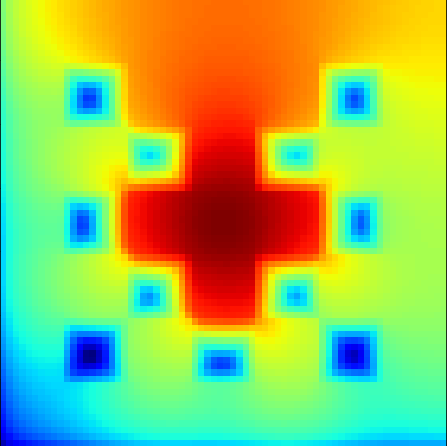
\includegraphics[width=0.66\columnwidth]{04_pn_method/results/p1_staggered_grid_asymmetric_bc.png}
\caption{$P_1$-solution.}
\label{fig:pn_staggering_asymmetry_bc_checkerboard}
\end{subfigure}
\caption{Dealing with staggered grid locations per voxel (left) implies a boundary interface which produces asymmetric results as seen for the solution of the checkerboard problem (right).}
\label{fig:pn_staggered_grid_unhandled_bc}
\end{figure}

The solution is to introduce additional unknowns to the system for every coefficient which is located in a boundary voxel as shown in figure~\ref{fig:pn_staggered_grid_handled_bc}\subref{fig:pn_staggering_correct_bc}. This will correct the location of the boundary interface and allows the same boundary conditions on opposite sides of the computational domain.
\begin{figure}[h]
\centering
\begin{subfigure}[t]{0.49\columnwidth}
\centering
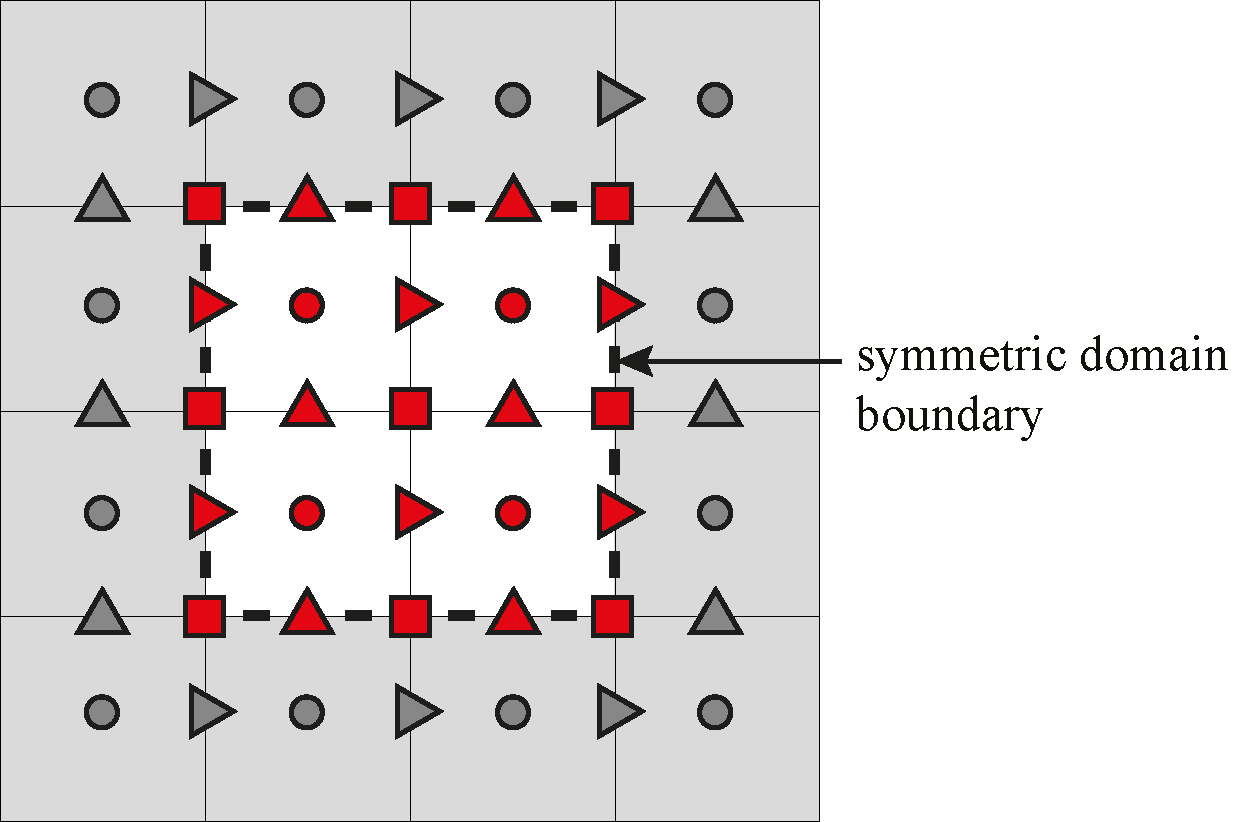
\includegraphics[width=1\textwidth]{04_pn_method/figures/fig_staggered_grid_domain_boundary_corrected.pdf}
\caption{Adjusted placement of staggered grid coefficients.}
\label{fig:pn_staggering_correct_bc}
\end{subfigure}
\hspace{0.01\columnwidth}
\begin{subfigure}[t]{0.34\columnwidth}
\centering
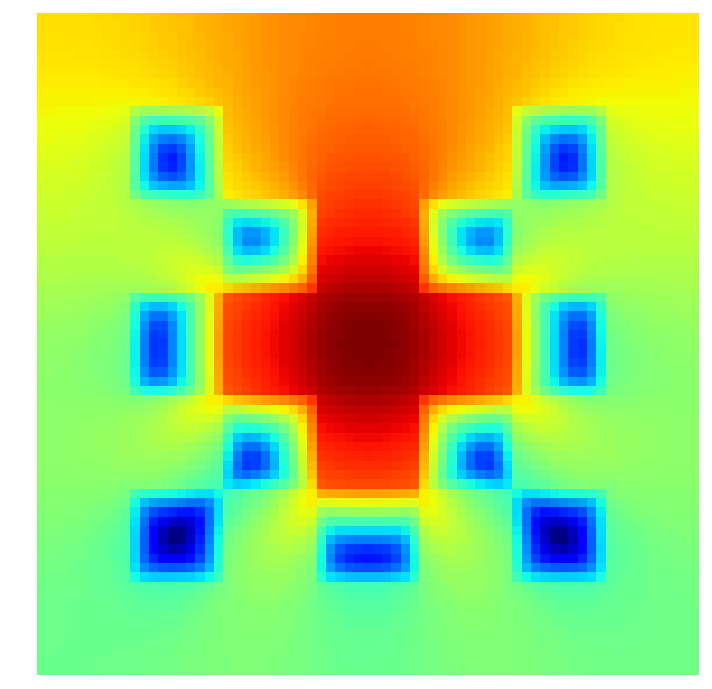
\includegraphics[width=\columnwidth]{04_pn_method/results/checkerboard2d_p5_neumann_staggered.png}
\caption{$P_1$-solution of the checkerboard problem.}
\label{fig:pn_staggering_correct_bc_checkerboard}
\end{subfigure}
\caption{Placing staggered grid coefficients such that the defined boundary interface is symmetric (left) leads to a correct symmetric solution of the checkerboard problem (right).}
\label{fig:pn_staggered_grid_handled_bc}
\end{figure}

The handling of boundary conditions is done by the solver framework. In order to support staggered grids, the stencil code will be generated with an additional function, which specifies the grid location of each coefficient. This function is used by the \emph{VoxelManager} to work out which additional unknowns are required. This results in complex management of indices of unknowns, as a simple indexing function is not sufficient anymore. Transparently handling this complexity is the purpose of the \emph{VoxelManager} class.

For client code applications, it is desirable to have all coefficients defined at the centers of voxels covering the problem domain. Therefore the solver framework offers an \emph{unstagger} function for staggered grids, which interpolates all coefficients at the voxel centers of the problem domain from the surrounding coefficient locations. Further the additional unknowns, which have been introduced to get correct boundary conditions, will be removed. This function converts a staggered grid solution vector to a collocated grid solution vector.

As shown in figure~\ref{fig:pn_staggering_correct_bc_checkerboard}, using the collocated grid from converting a staggered grid solution of a staggered grid solve, will produce a result free of oscillation and asymmetry artefacts.

\subsection{System Matrix and Solution}
\label{sec:pn_system_matrix}

After initializing the \emph{PNSystemBuilder} object matrix with the \emph{Stencil} and \emph{Scene}, the system matrix $A$ and right hand side vector $\vec{b}$ are built and made available to the client code, which will use it to solve for the solution vector $\vec{u}$. The solver developed as part of this thesis uses Eigen~\cite{Eigen}, but any other linear algebra package with standard methods available is applicable too. 

However, the system matrix $A$, when generated from the $P_N$-equations, has properties that restrict the application of methods for solving the system. The number of rows and columns of $A$ is determined by the total number of voxels in the computational domain, multiplied by the number of spherical harmonics coefficients per voxel. The matrix is squared and sparse due to the local structure of the discretization and coupling. Unfortunately, the system matrix $A$ is non-symmetric (due to the transport term) and not diagonal dominant, which together rules out many iterative methods for solving linear systems.
\begin{figure}[h]
\centering
%\missingfigure{structure of the system matrix and solution vector (the figure from the paper)}
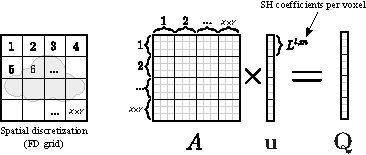
\includegraphics[width=0.75\textwidth]{04_pn_method/figures/fig_matrix_layout.pdf}
\caption{Structure of coefficient matrix $A$ and solution vector $\vec{u}$ after discretization of the $P_N$-equations on a finite difference grid.}
\label{fig:pn_matrix_layout}
\end{figure}

Some standard methods, such as LU-decomposition, QR-decomposition or Singular-value decomposition allow for solving systems of linear equations with non-symmetric coefficient matrices $A$ and are applicable to solving the system generated by the $P_N$-solver. 

Due to the asymmetry in $A$, applying iterative methods becomes a challenge. While iterative methods exist for non-symmetric matrices (based on Arnoldi iterations), these methods are more complex and tend to require more memory, that furthermore linearly grows with each operation. So only a limited number of iterations can be done before a restart becomes necessary.

Instead, iterative methods can be applied more easily by solving the normal form
\begin{align}
A^TA\vec{u} = A^T\vec{b}\ .
\end{align}
This gives a symmetric and positive definite system matrix $A^TA$, albeit with a higher condition number. Investigation of other solution schemes (e.g. multigrid) would be an interesting avenue for future work.

However, more importantly, in the presence of vacuum regions, matrix $A$ becomes singular and the system cannot be solved at all. The intuition behind this behavior is that in case of vacuum, the collision and scattering terms vanish completely, leaving the transport operator to exclusively define the solution. Since the transport operator only defines the relationship between unknowns in terms of their derivatives, it becomes clear that this is not enough information to constitute a unique solution. This is best exemplified by looking at a minimal version of that problem:
\begin{align*}
\frac{df\left(x\right)}{dx} = b\left(x\right)
\end{align*}
This differential equation imposes a constraint on the derivative of the solution, which is unique up to a constant factor. Hence there are infinitely many solutions. Therefore, there is no unique solution to this problem and hence the matrix $A$ after discretization will be singular.

A way out of this problem is to specify additional boundary conditions. However, for problems of simple complexity, this would already amount to finding a solution to the problem in the first place.

A simple alternative to which this thesis refers back is minimum thresholding. A minimum threshold value $\sigma_{min}$ is specified by the user. That threshold value is returned for any extinction value that falls below that threshold. This amounts to adding an ambient extinction medium by which vacuum regions are avoided completely and which causes the system to never become singular. Let $\sigma_{ot}$ be the original extinction coefficient coming from the input dataset. Unless stated otherwise, throughout this thesis the extinction coefficient is defined to be
\begin{align}
\label{eq:pn_solver_minimum_threshold}
\sigma_t\left(\vec{x}\right) =
\begin{cases}
\sigma_{ot}\left(\vec{x}\right), & \text{for $\sigma_{ot}\ge\sigma_{min}$}
\\
\sigma_{min}, & \text{otherwise}
\end{cases}
\end{align}

This concludes the section on the $P_N$-solver and its system components.
\section{Integration into Rendering Software}
\label{sec:pn_rendering_integration}

This section will explain in detail how the solver and its result can be integrated and used in a standard rendering framework.

The solver framework is encapsulated using the \emph{PNSystemBuilder} class and therefore, can be easily migrated from a standalone application into any rendering framework. As outlined in section~\ref{sec:pn_framework}, references to a \emph{Stencil} class and the \emph{Scene} class are needed to create a \emph{PNSystemBuilder} instance.

The truncation order $N$ is a user parameter, which ideally is decided at runtime. However, the stencil code will always be the same for a given truncation order $N$, since it has been generated independently of grid resolution, boundary conditions and radiative transfer parameters. It suggests itself to precompute and precompile the stencil code for all possible options for $N$. The rendering framework is compiled once with all possible stencil codes. As soon as the user decided, which truncation order $N$ to use, a \emph{Stencil} class is generated using the function pointers of the respective compiled stencil code functions.

The \emph{Scene} class is also created by the rendering framework. It will be populated with references to \emph{Field} classes for radiative transfer quantities, such as extinction, albedo, emission and phase function. The \emph{Field} classes serve as adapter pattern according to Gamma et al.~\cite{Gamma95} and can be used to feed arbitrary representations of spatially varying scalar fields, as input to the solver framework.

An important aspect of providing inputs to the solver is the emission term, which describes the illumination within the problem domain. Light sources, which illuminate the volume from outside, will have to be expressed as emission on the boundary interface and light sources inside the problem domain, such as point- or area lights need to be rasterized into the emission field. Expressing outside illumination at the boundaries potentially conflicts with the boundary conditions, which cause the solution near the boundary to be less accurate. Rasterizing light sources inside the domain will be challenging for the solver, if strong directionality is present. The cause is the spherical harmonics approximation that has difficulties representing delta or strongly directional functions in angular domain due to truncation of higher frequency moments.

To alleviate the challenges of light sources with strong directionality, the rendering system, developed as part of this thesis, implements an idea, which is inspired by Grosjean’s analytical approximation to exact transport of a point light source within a homogeneous medium (Grosjean~\cite{Grosjean56}). Instead of providing an approximation to the full light transport caused by the point light, the approximation separates the unscattered light from the scattered light. The solution for the unscattered contribution is exact and an approximation is needed only for the scattered light. This approach is reasonable as the light contribution from scattered light has more energy in the lower frequencies due to the phase function, which acts as a convolution filter on the radiance function in angular domain.

Following this idea by Grosjean, the radiance field $L$ is separated into unscattered light $L_{u}$ and multiple scattered light $L_m$:
\begin{align}
L\left(\vec{x}, \omega\right) = 
L_u\left(\vec{x}, \omega\right)
+L_m\left(\vec{x}, \omega\right)
\end{align}

The unscattered light is the contribution of the radiance field, which did not undergo any scattering events. Therefore, it satisfies the following restricted radiative transfer equation, where the scattering term vanished:
\begin{align}
\left(\nabla\cdot\omega\right)L_u\left(\vec{x}, \omega \right)
=
-\sigma_t\left(\vec{x}\right) L_u\left(\vec{x}, \omega \right)
\label{eq:restricted_rte}
\end{align}


When replacing the radiance field $L$ with the decomposition above in the radiative transfer equation (equation~\ref{eq:rte}) the result is:
\begin{align}
\left(\nabla\cdot\omega\right)L_u\left(\vec{x}, \omega \right)
+\left(\nabla\cdot\omega\right)L_m\left(\vec{x}, \omega \right)
=&
-\sigma_t\left(\vec{x}\right) L_u\left(\vec{x}, \omega \right)
\nonumber\\
&
-\sigma_t\left(\vec{x}\right) L_m\left(\vec{x}, \omega \right)\nonumber\\
&
\underbrace
{
+\sigma_s\left(\vec{x}\right) \int_{\Omega}
{
\phase\left(\omega'\cdot\omega\right)L_u\left(\vec{x}, \omega' \right)\ud\omega'
}
}_{L_s}
\nonumber\\
&
+\sigma_s\left(\vec{x}\right) \int_{\Omega}
{
\phase\left(\omega'\cdot\omega\right)L_m\left(\vec{x}, \omega' \right)\ud\omega'
}
\nonumber
\\
&
+Q_e\left(\vec{x}, \omega\right)
\nonumber
\  .
\end{align}

By using equation~\ref{eq:restricted_rte}, the extinction terms for the unscattered light can be cancelled out, producing the medium radiative transfer equation:
\begin{align}
\left(\nabla\cdot\omega\right)L_m\left(\vec{x}, \omega \right)
=&
-\sigma_t\left(\vec{x}\right) L_m\left(\vec{x}, \omega \right)\nonumber\\
&
+\sigma_s\left(\vec{x}\right) \int_{\Omega}
{
\phase\left(\omega'\cdot\omega\right)L_m\left(\vec{x}, \omega' \right)\ud\omega'
}
\nonumber
\\
&
\underbrace
{
+L_s\left(\vec{x}, \omega\right)
+Q_e\left(\vec{x}, \omega\right)
}_{Q}
\nonumber
\  .
\end{align}
The quantity $L_s$ is the single scattered light, which is folded together with the volume emission $Q_e$ into the general emission term $Q$.

Using the emission term $Q$, the medium radiative transfer equation is solved, using the $P_N$-method previously described. The solution vector $\vec{u}$ is brought into collocated form, using the \emph{unstaggering} function described in section~\ref{sec:pn_staggered}. This allows straightforward subsequent use in a rendering system for image generation. 

The solution vector provided by the solver contains a set of spherical harmonics coefficients for every voxel of the computational grid. This set of coefficients describes the spherical radiance function at the voxelcenter. The framework, which has been developed as part of this thesis, provides a \emph{PNSolution} class that is a voxelgrid of $K$-dimensional vectors. The number of vector elements $K$ is the number of spherical harmonics coefficients, which is driven by the truncation order of the $P_N$-equations. The radiance field is reconstructed by first interpolating all coefficients at the given worldspace position from the coefficients at surrounding voxels, followed by computing the spherical harmonics reconstruction in equation~\ref{eq:sh_real_reconstruction}.

In this thesis, images will be rendered from the solution directly. An alternative route could be to use the solution in combination with one of the variance reduction techniques outlined in section~\ref{sec:foundations_mc}.

Volume rendering frameworks are concerned with solving the radiative transfer equation~\ref{eq:rte}. In order to integrate the solution of the medium radiative transfer equation, the inscattering term in the radiative transfer equation has to be split and the medium radiance $L_m$ is replaced by its truncated spherical harmonics reconstruction $\widehat{L}_m$:
\begin{align}
\left(\nabla\cdot\omega\right)L\left(\vec{x}, \omega \right)
=&
-\sigma_t\left(\vec{x}\right) L\left(\vec{x}, \omega \right)\nonumber\\
&
+\sigma_s\left(\vec{x}\right) \int_{\Omega}
{
\phase\left(\omega'\cdot\omega\right)\left(L_u\left(\vec{x}, \omega' \right)+\widehat{L}_m\left(\vec{x}, \omega' \right)\right)\ud\omega'
}
\nonumber
\\
&
+Q_e\left(\vec{x}, \omega\right)
\nonumber
\\
=&
-\sigma_t\left(\vec{x}\right) L\left(\vec{x}, \omega \right)
\nonumber\\
&
+\sigma_s\left(\vec{x}\right) \int_{\Omega}
{
\phase\left(\omega'\cdot\omega\right)L_u\left(\vec{x}, \omega' \right)\ud\omega'
}
\nonumber\\
&
+\sigma_s\left(\vec{x}\right) \int_{\Omega}
{
\phase\left(\omega'\cdot\omega\right)\widehat{L}_m\left(\vec{x}, \omega' \right)\ud\omega'
}
\nonumber\\
&
+Q_e\left(\vec{x}, \omega\right)
\label{eq:pn_rendering_integration1}
\end{align}
When seperating the radiance field and using the single scattered light as emission term for the $P_N$-method, this equation needs to be solved to fully account for the radiance field. Any Monte-Carlo method would need to integrate the single scattered light (e.g. by doing next event estimation). The indirect or multiple scattered light is accounted for by integrating over the angular dependent $P_N$-solution and weighting it by the phase function and scattering term to account for the inscattering of indirect illumination.

If the phase function is isotropic, then equation~\ref{eq:pn_rendering_integration1} further simplifies to
\begin{align}
\left(\nabla\cdot\omega\right)L\left(\vec{x}, \omega \right)
=&
-\sigma_t\left(\vec{x}\right) L\left(\vec{x}, \omega \right)
+\sigma_s\left(\vec{x}\right) \int_{\Omega}
{
\phase\left(\omega'\cdot\omega\right)L_u\left(\vec{x}, \omega' \right)\ud\omega'
}
\nonumber\\
&
+
\frac{1}{4\pi}
\sigma_s\left(\vec{x}\right)
\int_{\Omega}
{
\widehat{L}_m\left(\vec{x}, \omega' \right)\ud\omega'
}
+Q_e\left(\vec{x}, \omega\right)
\nonumber\\
=&
-\sigma_t\left(\vec{x}\right) L\left(\vec{x}, \omega \right)
+\sigma_s\left(\vec{x}\right) \int_{\Omega}
{
\phase\left(\omega'\cdot\omega\right)L_u\left(\vec{x}, \omega' \right)\ud\omega'
}
\nonumber\\
&
+
\frac{1}{4\pi}
\sigma_s\left(\vec{x}\right)
L_m^{0,0}\left(\vec{x}\right)
+Q_e\left(\vec{x}, \omega\right)
\ ,
\label{eq:pn_rendering_integration2}
\end{align}
due to zero moment property of the radiance field $\int_{\Omega}\widehat{L}_m\ud\omega'=L_m^{0,0}$.

Figure~\ref{fig:pn_rendering_integration_overview} gives a schematic overview over how the method is integrated into a rendering framework. The single scattered light is precomputed and projected into the emission term for the $P_N$-solver. Together with the other discretized radiative transfer parameters, the $P_N$-solution is obtained. The final image is generated by path tracing to the first bounce into the volume, and by computing the inscattered uncollided light (either by using Monte Carlo integration or by using the precomputed single scattered light, which was used as emission term for the $P_N$-solver). Instead of continuing tracing the path to account for indirect illumination, a separate inscattering integral is computed over the multiple scattered light from the $P_N$-solution.

\begin{figure}[h]
\centering
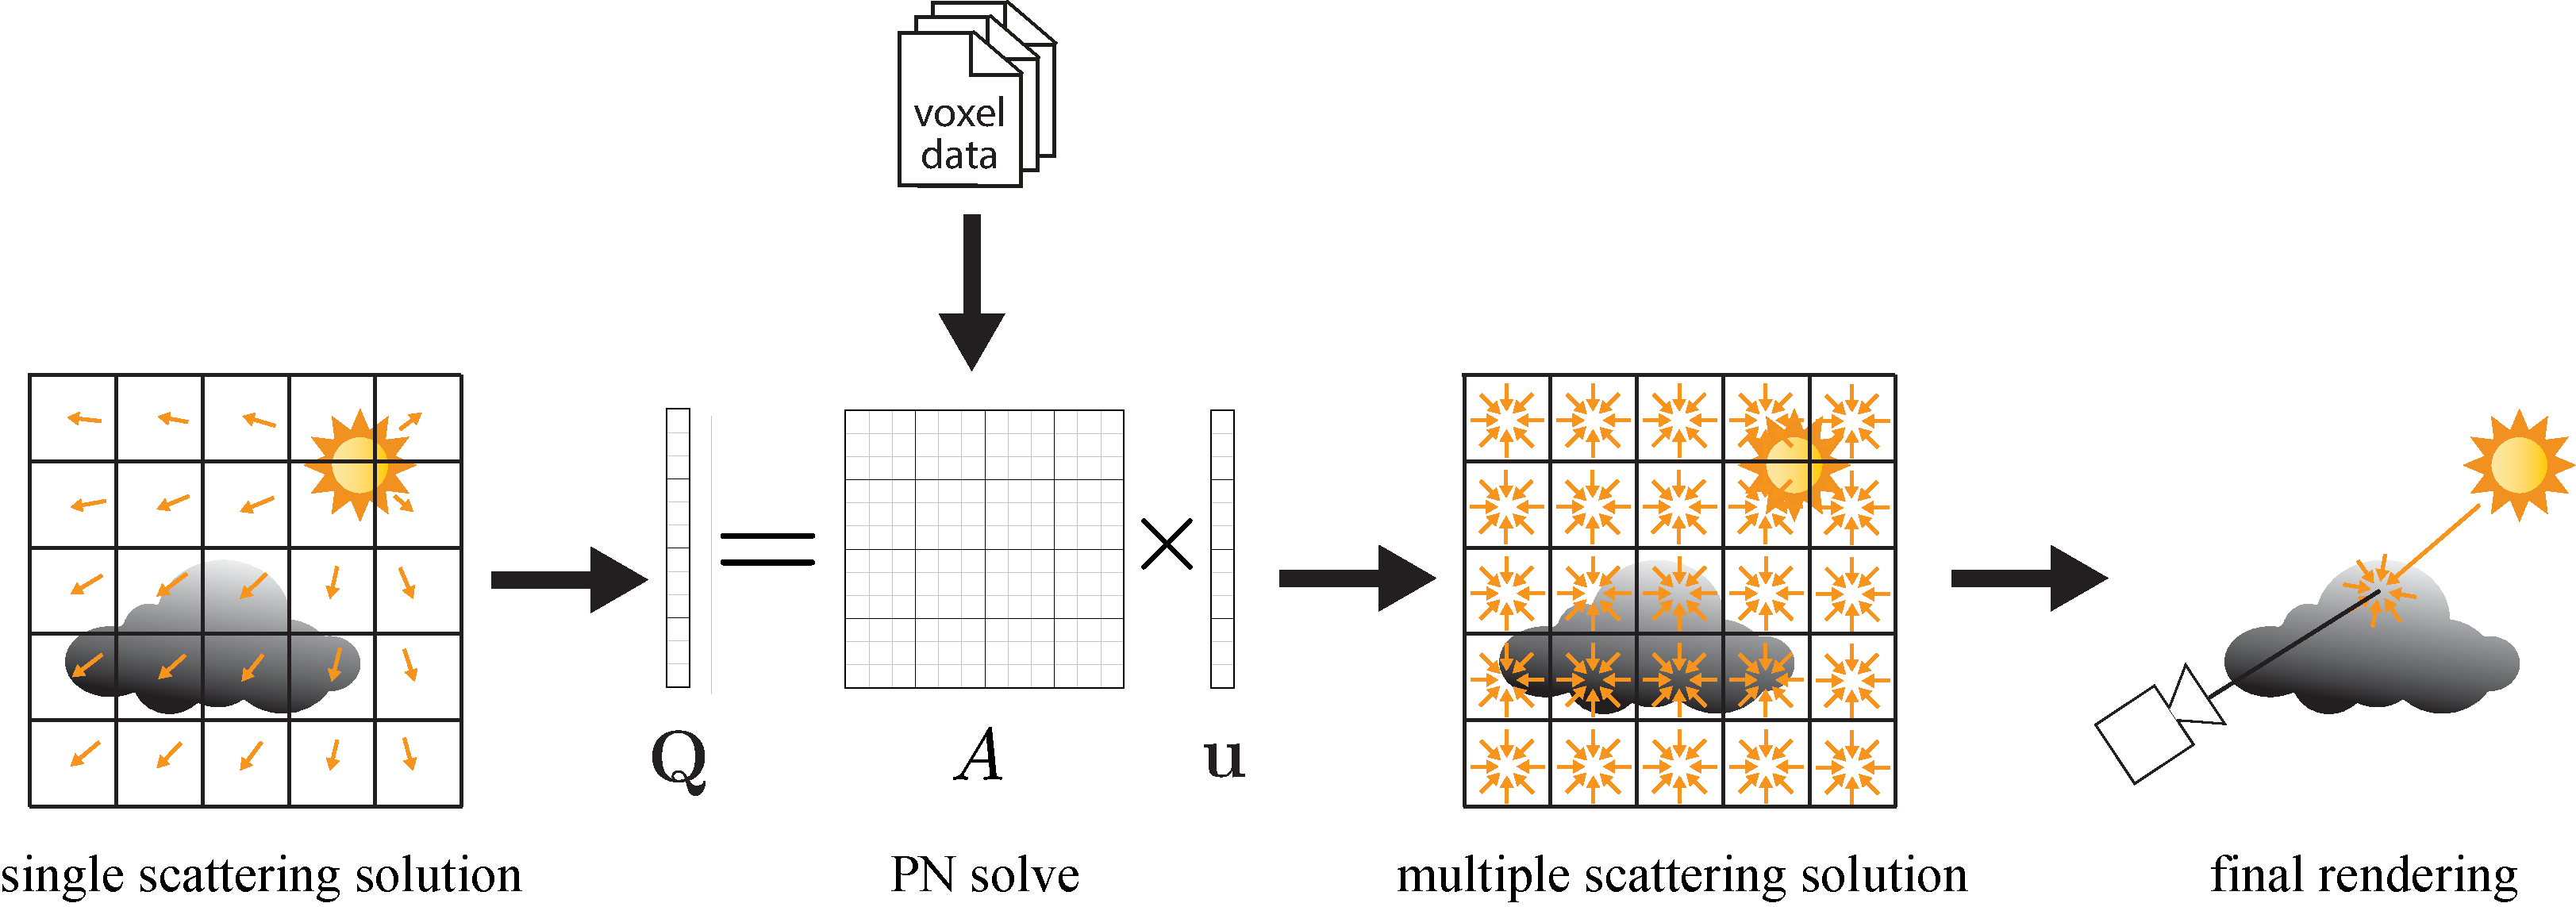
\includegraphics[width=0.99\textwidth]{04_pn_method/figures/fig_rendering_pipeline.pdf}
%\missingfigure{show high level picture of a rendering system. input data. precomputation. rasterization. synthesis of first order scattering and higher order scattering}
\caption{Overview over the full rendering process. The single scattering solution is precomputed and projected into RHS $Q$. The coefficient matrix $A$ is assembled from voxelized RTE quantities and used to compute solution $u$. That solution is then un-projected and used to evaluate the multiple scattering contribution during final rendering step.}
\label{fig:pn_rendering_integration_overview}
\end{figure}

After having outlined how the $P_N$-Method and its solution can be integrated into a rendering application, concrete results will be shown and discussed in the following section.

\section{Results}
\label{sec:pn_results}

After outlining the $P_N$-solver in section~\ref{sec:pn_solver} and its integration into a rendering framework in the previous section, this section will give and discuss results produced by the system, which was developed as part of this thesis.

\subsection{Point Source Problem}
\label{sec:pn_results_pointsource}

The point source problem is a canonical problem, which is well-suited to validate the method and assess its accuracy. The problem is simple, and an analytical solution exists to allow comparison against the ground truth (section~\ref{sec:foundations_analytical}). The medium is homogeneous with infinite extent. This is approximated for the solver by a unit cube. The emission term is an ideal unit power point light with isotropic emission in angular domain and a delta function in spatial domain. This delta function is discretized into the finite difference grid by distributing its unit power over the volume of a single voxel:
\begin{align}
Q_{ijk} = \frac{1}{h_xh_yh_z}
\end{align}
The index {ijk} refers to the voxel, in which the point light is located.

Note that here the radiance field is not seperated as outlined in section~\ref{sec:pn_rendering_integration}. The emission field represents only the discretized light source and therefore, the resulting discretized radiance field represents all light transport, including single scattered light.

The correct analytical solution for fluence is given by D'Eon et al.~\cite{dEon11}. The authors also introduce a very accurate approximation, called the Grosjean solution, which is simpler to evaluate and always convergent. The fluence is identical to the zero coefficient of the spherical harmonics expansion of the radiance field ($L^{0,0}$), which shall be can compared directly with the Grosjean solution.
\begin{figure}[h]
\centering
%\missingfigure{pointsource plots PN}
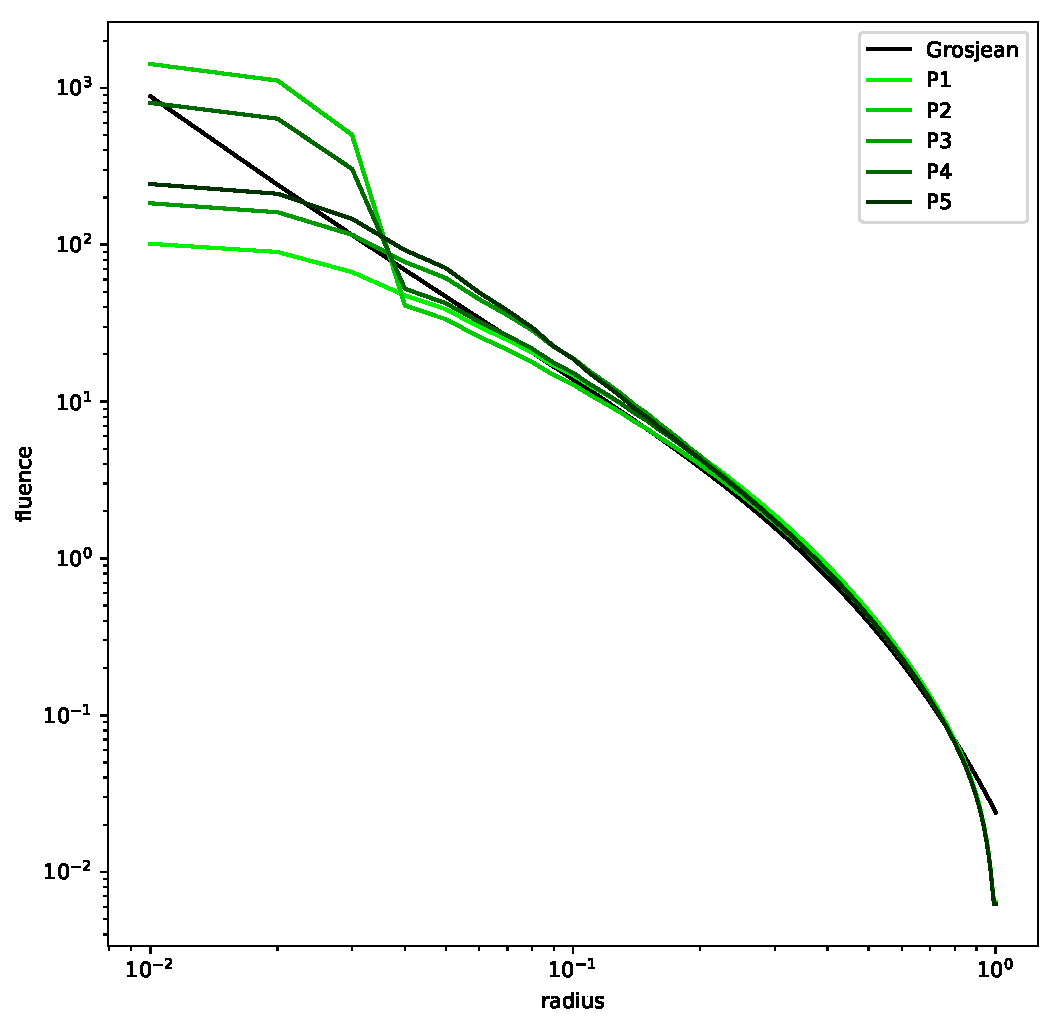
\includegraphics[width=0.7\textwidth]{04_pn_method/results/pointsource_pn.pdf}
\caption{Comparison of $P_N$-results for the pointsource problem with different truncation order $N$ against groundtruth solution (Grosjean). The disagreement on the right comes from zero dirichlet boundary conditions.}
\label{fig:pn_results_pointsource_1}
\end{figure}
Figure~\ref{fig:pn_results_pointsource_1} compares the solution for $P_1$, $P_2$, $P_3$, $P_4$, $P_5$ against the Grosjean solution. The figure shows that with higher $N$, the $P_N$-solution increases in accuracy. Also noticeable is that with increasing truncation order $N$, the $P_N$-solution oscillates around the exact solution and approaches it with alternating under- and overestimation, especially near the point source. Even truncation order will overestimate and odd truncation order will produce an underestimate. The performance characteristics are given in table~\ref{tab:results_pointsource}

\begin{table}[!h]
	\centering
	\caption{Performance characteristics of the $P_N$-method for the point source problem for a $64\times64\times64$ sized grid.}
	\label{tab:results_pointsource}
	% \flushleft
	\begin{tabular}{l r r r}
    \hline
	Truncation order \textbf{N}
    & 1 & 3 & 5
    \\
    \hline
    Number of rows/columns in $A$
    & 1.048.576 & 4.194.304 & $9.437.184$
    \\
    Size of linear system (in MB)
    & $8.4$ & $33.5$ & $75.5$
    \\
    Solve time (in min)
    & 10 & 21 & 45
	\end{tabular}
\end{table}

\subsection{Checkerboard Problem}
\label{sec:pn_results_checkerboard}

The checkerboard problem is a two-dimensional setup solved by the two-dimensional $P_N$-equations, introduced in section~\ref{sec:pn_2d}. This problem is known to the nuclear science field and is used across literature to compare and validate implementations of deterministic methods. It consists of absorbing regions, which are embedded in a scattering medium and arranged in a checkerboard pattern. An emitting region is located in the center square.

Running the $P_N$-method on the checkerboard problem, allows to compare it against the \textsf{StaRMAP} solver by Seibold et al.~\cite{Seibold14}. Their solver solves the time-dependent $P_N$-equations and employs a time-stepping scheme, for which a step-size and a target time has to be specified. In contrast, the solver, which has been introduced in this thesis, solves for the steady-state solution of the real-valued $P_N$-equations using a global linear system. No step-size or duration parameters are required. The $P_N$-method will be used on the checkerboard problem for $N=5$. The results from \textsf{StaRMAP} have been generated by setting a long duration and a small step-size to get an accurate and close-to steady state result.
\begin{figure}[h]
\centering
\begin{subfigure}{0.49\columnwidth}
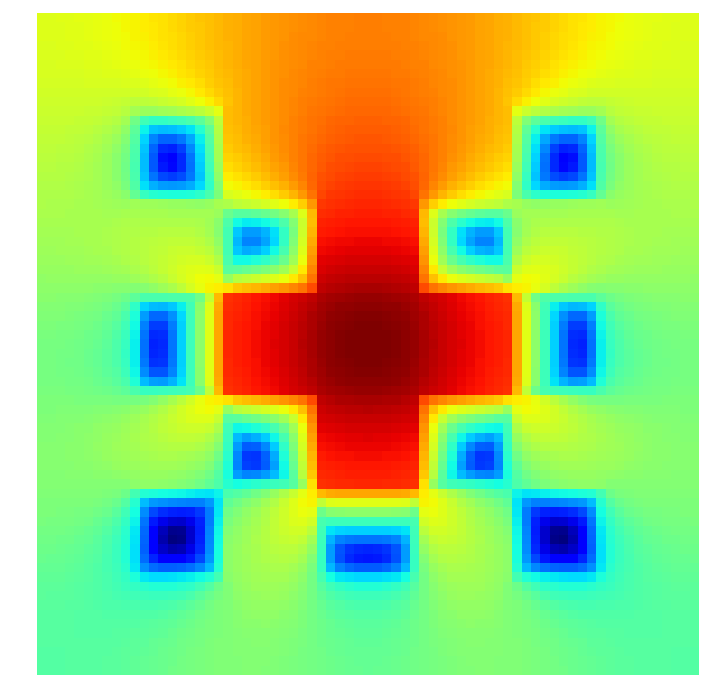
\includegraphics[width=\columnwidth]{04_pn_method/results/checkerboard2d_p5_neumann_staggered_starmap.png}
%\missingfigure{checkerboard p5}
%\caption{?}
%\label{fig:pn_results_nebulae1_pathtraced}
\end{subfigure}%
\hspace{0.01\columnwidth}
\begin{subfigure}{0.49\columnwidth}
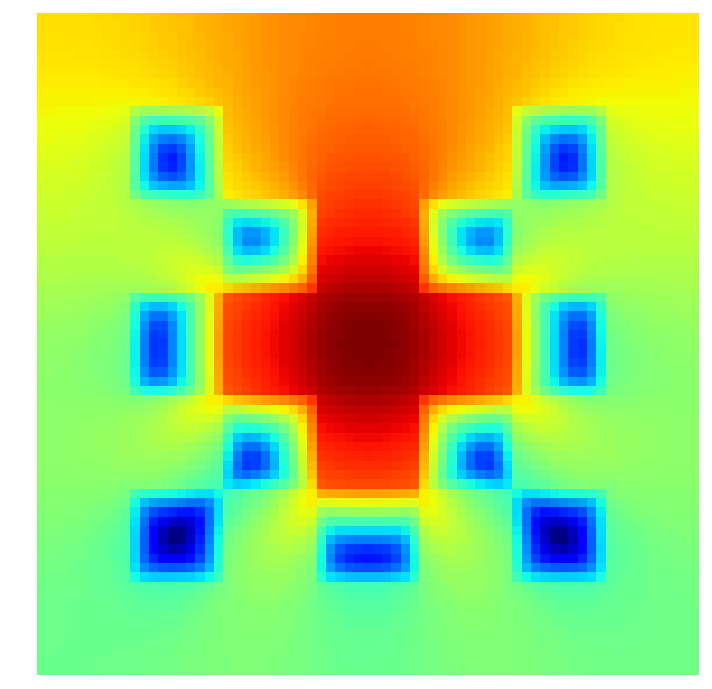
\includegraphics[width=\columnwidth]{04_pn_method/results/checkerboard2d_p5_neumann_staggered.png}
%\missingfigure{checkerboard p5 starmap}
%\caption{?}
%\label{fig:pn_results_nebulae1_P1}
\end{subfigure}%
%\vspace{-0.2in}
\caption{Solver $P_5$-result for the checkerboard problem (left) in comparsison to \textsf{StaRMAP} by Seibold et al.~\cite{Seibold14} (right). The solution of the solver, developed as part of this thesis, is in very good agreement.}
\label{fig:pn_results_checkerboard1}
\end{figure}

\subsection{Procedural Cloud}
\label{sec:pn_results_clouds}

In a more practical example the $P_N$-solver is used to compute the multiple scattered light in a procedurally generated cloud dataset, which is being illuminated by a directional cloud. The radiance field is separated into single scattered and multiple scattered light as explained in section~\ref{sec:pn_rendering_integration} and a basic forward path tracer (section~\ref{sec:foundations_mc}) is used to trace camera rays and integrate single scattered light according to equation~\ref{eq:pn_rendering_integration1}.

Characteristic about the dataset is the presence of very dense media embedded in regions of very low density and vacuum (zero extinction), which exhibits very strong density gradients. The presence of vacuum has a signficiant effect on the convergence behaviour of the $P_N$-method as explained in section~\ref{sec:pn_system_matrix}. The convergence deteriorates in the presence of very low density regions. The coefficient matrix $A$ becomes singular, when regions of pure vacuum exist in the dataset.

The $P_N$-method for $N={1,2,3,4,5}$ has been run using a minimum threshold of $\sigma_{min}=1.0e^{-3}$. The resolution of the finite difference grid used by the $P_N$-method is $64\times 64\times 64$. Separating the multiple scattered light from the single scattered light has the benefit that the multiple scattered light has lower frequencies, which allows using a coarser finite difference grid without a significant loss of accuracy.
\begin{figure}[h]
\centering
\begin{subfigure}{0.49\columnwidth}
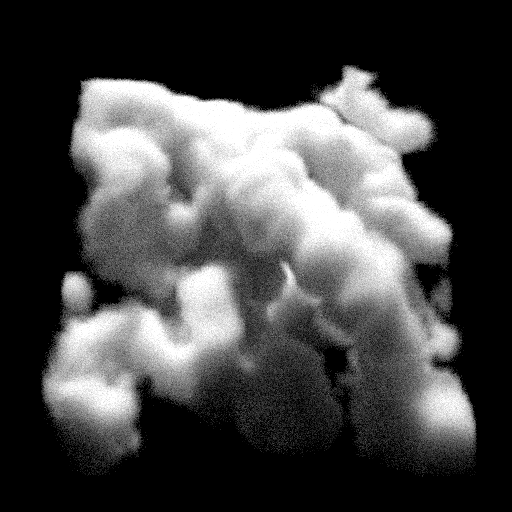
\includegraphics[width=\columnwidth]{04_pn_method/results/nebulae_ms_groundtruth.png}
%\missingfigure{nebulae pathtraced}
\caption{Pathtraced}
\label{fig:pn_results_nebulae1_pathtraced}
\end{subfigure}%
\hspace{0.01\columnwidth}
\begin{subfigure}{0.49\columnwidth}
%\includegraphics[width=\columnwidth]{images/checkerboard2d_p1_neumann_staggered.png}
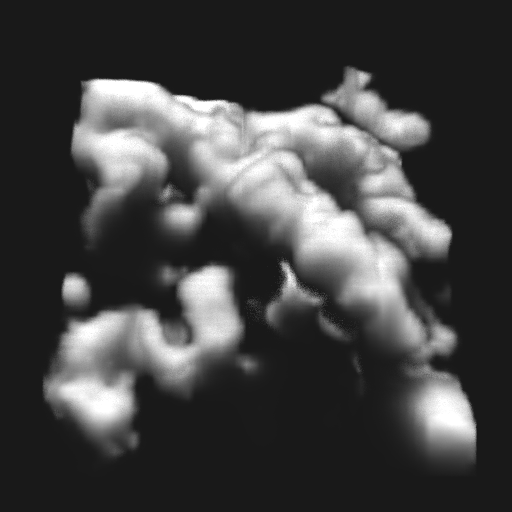
\includegraphics[width=\columnwidth]{04_pn_method/results/nebulae_p1_ms.png}
%\missingfigure{nebulae P1}
\caption{$P_1$}
\label{fig:pn_results_nebulae1_P1}
\end{subfigure}%

\begin{subfigure}{0.49\columnwidth}
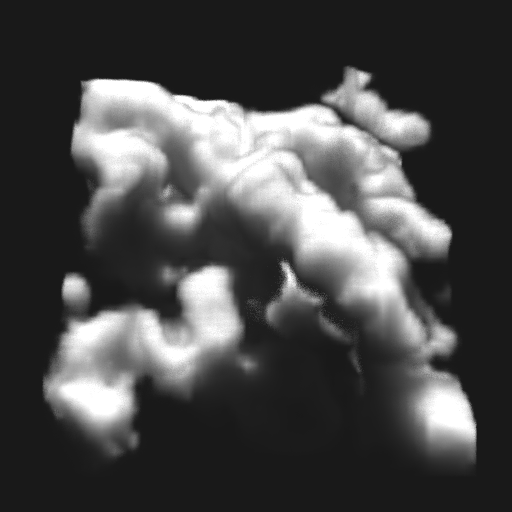
\includegraphics[width=\columnwidth]{04_pn_method/results/nebulae_p3_ms.png}
%\missingfigure{nebulae P3}
\caption{$P_3$}
\label{fig:pn_results_nebulae1_P3}
\end{subfigure}%
\hspace{0.01\columnwidth}
\begin{subfigure}{0.49\columnwidth}
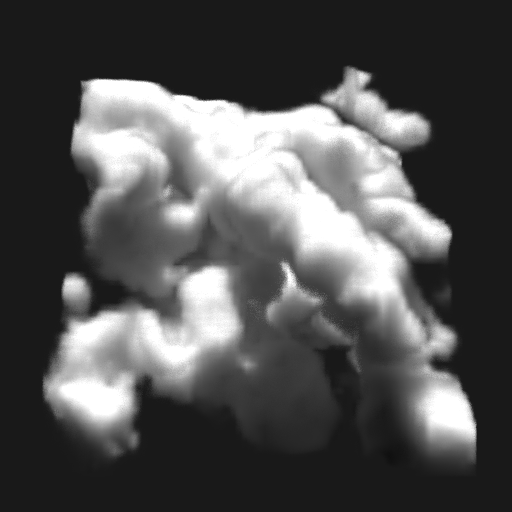
\includegraphics[width=\columnwidth]{04_pn_method/results/nebulae_p5_ms.png}
%\missingfigure{nebulae P5}
\caption{$P_5$}
\label{fig:pn_results_nebulae1_P5}
\end{subfigure}%

%\vspace{-0.2in}
\caption{$P_N$-results for the procedural cloud dataset (multiple scattered light) with different truncation order $N$.}
\label{fig:pn_results_nebulae1}
\end{figure}

The results for the procedural cloud problem are shown in figure~\ref{fig:pn_results_nebulae1}. As expected, the increase of the truncation order improves the accuracy of the solution. Especially the regions at the bottom of the cloud, which only receive indirect light are better resolved with higher $N$. However, with the increase of the truncation order, the size of the system increases and requires longer time to converge.

\begin{table}[!h]
	\centering
	\caption{Performance characteristics of the $P_N$-method for the procedural cloud problem for a $64\times64\times64$ sized grid with a minimum extinction coefficient threshold of $4$.}
	\label{tab:results_cloud}
	% \flushleft
	\begin{tabular}{l r r r}
    \hline
	Truncation order \textbf{N}
    & 1 & 3 & 5
    \\
    \hline
    Number of rows/columns in $A$
    & 1.048.576 & 4.194.304 & $9.437.184$
    \\
    Size of linear system (in MB)
    & $8.4$ & $33.5$ & $75.5$
    \\
    Solve time (in s)
    & 9 & 14 & 20
	\end{tabular}
\end{table}

The performance characteristics shown in table 
~\ref{tab:results_cloud} are heavily driven by the presence of low density or vacuum regions. In case of vacuum regions specifically, the condition number is singular. In that case the residual flattens and the solver actually never really converges below a certain error value. Therefore application of a minimum threshold for the extinction coefficient $\sigma_t$ becomes necessary. With a sufficiently high threshold (relative to the length scale of the problem), computation times can be reduced drastically while compromising on the discrepancy to the original problem containing vacuum regions. In figure~\ref{fig:pn_results_convergence} the convergence behaviour for solving the normal form using the conjugate-gradient method is being compared for different choices of the threshold $\sigma_{min}$.
\begin{figure}[h]
\centering
%\missingfigure{convergence}
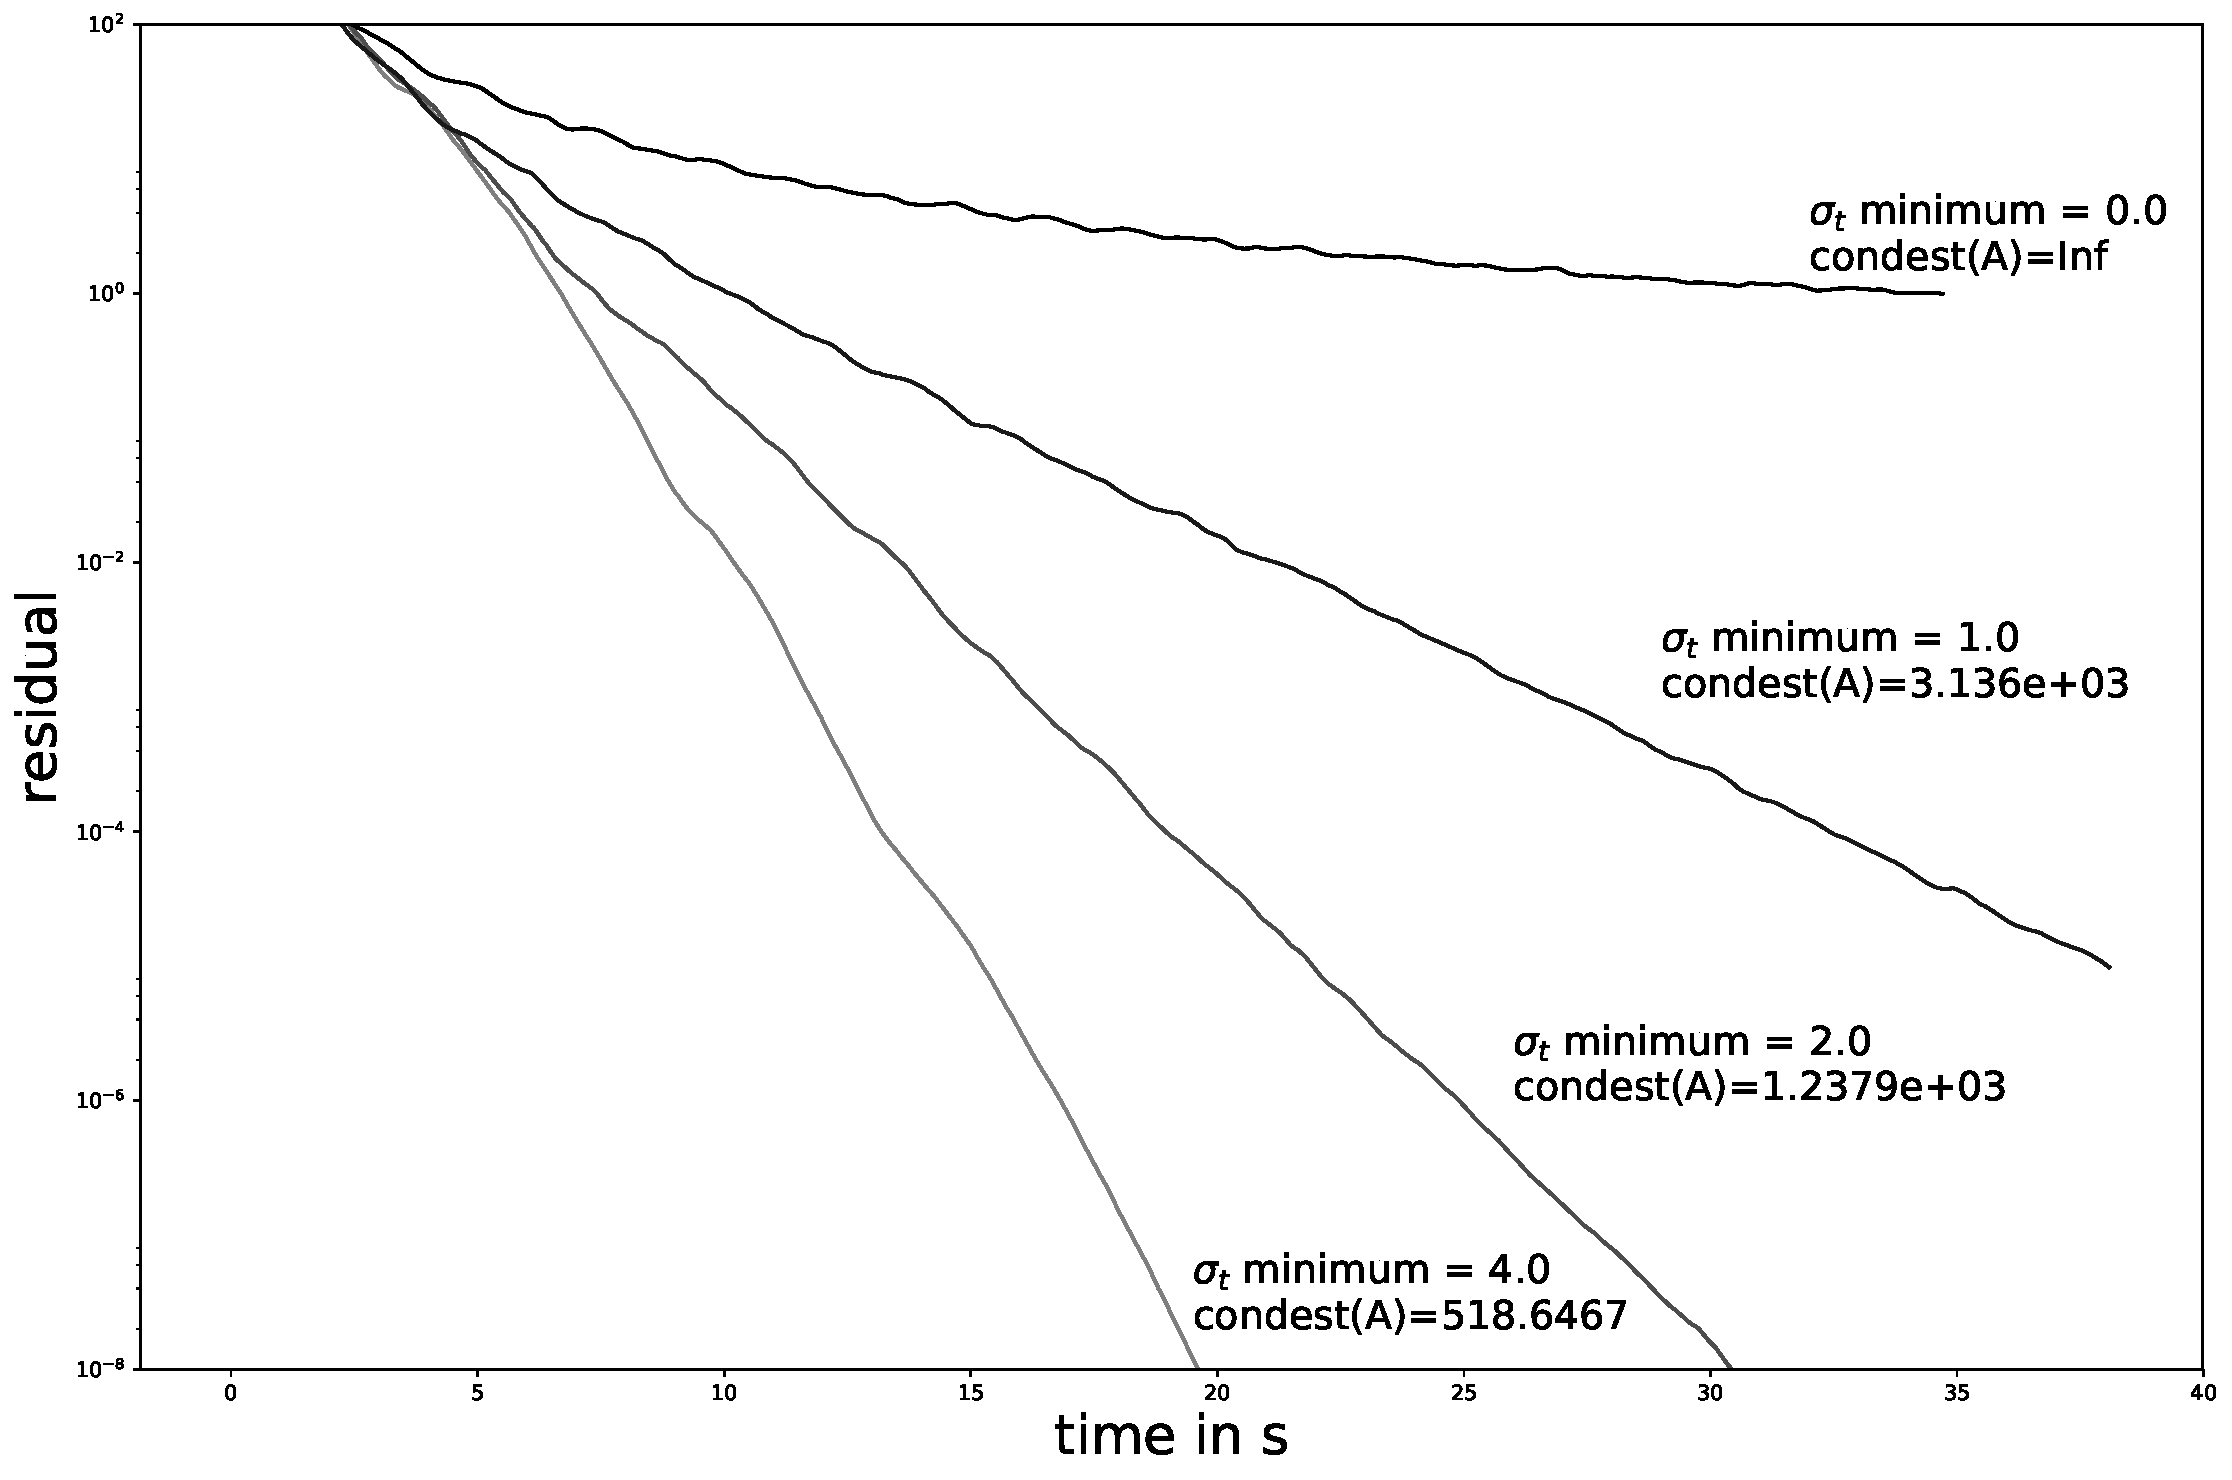
\includegraphics[width=\columnwidth]{04_pn_method/results/fig_nebulae_p1_convergence.pdf}
\caption{Convergence of $P_5$ for different choices of minimum threshold $\sigma_{min}$ and its effect on the conditional number for the coefficient matrix $A$.}
\label{fig:pn_results_convergence}
\end{figure}

For rendering of clouds and other participating media in computer graphics, vacuum or low density regions are of great importance. In these scenarios, the $P_N$-method is not competitive when compared to other techniques.







\section{Discussion}

The solver, which has been introduced in this chapter produces results that are in good agreement with radiative transfer ground truth solutions. This has been demonstrated with the point source problem in section~\ref{sec:pn_results_pointsource}. The results for the checkerboard problem (section~\ref{sec:pn_results_checkerboard}) are in very good agreement with results from deterministic methods in other fields. This further demonstrates the correct derivation of the real-valued $P_N$-equations and implementation of the solver, developed as part of this thesis.

The procedural cloud results in section~\ref{sec:pn_results_clouds} show that in order to capture light in the visually important indirect regions of the dataset, truncation orders of $N=5$ or higher are necessary. The computation time and memory requirements in this case are signficiant as seen in table~\ref{tab:results_cloud}. These are very heavy requirements, which will limit the use of the $P_N$-method in practical applications. The next chapter covers the Diffusion Approximation, which has been introduced to computer graphics by Stam~\cite{Stam95}. It is derived as a degenerated case of the $P_1$-equations and reduces to an uncomplicated diffusion equation.
\chapter{Diffusion Approximation for Multiple Scattering in Participating Media}
%
\label{sec:diffusion_approximation}

In the previous chapter the angular variable of the radiative transfer equation was discretized into a set of coupled partial differential equations, the $P_N$-equations. Further a method has been introduced for discretizing these equations into a system of linear equations which could be solved using standard methods. Since the number of equations depends on the truncation order $N$, higher $N$ will result in increasingly larger systems. The results showed that the amount of computational resources required makes this approach very unattractive for practical rendering applications, especially for higher $N$ (see section~\ref{sec:pn_results}). This chapter recaps the diffusion approximation, a theory which is being derived from the general $P_N$-equations with a truncation order of $N=1$. It is particularly appealing because it reduces to a simple diffusion equation which can be solved very efficiently. This theory therefore is an important step in trying to derive a practical deterministic method from the spherical harmonics expansion of the radiative transfer equation.

The diffusion approximation has been introduced to computer graphics by Stam~\cite{Stam95} for dealing with multiple scattering in participating media. Therefore the theory and method for solving it is not new. However, in this thesis a complete chapter is dedicated to this theory for two reasons. First the idea of this thesis is to present a comprehensive picture on spherical harmonics methods and diffusion approximation is a very popular and important part of it. The second reason is that diffusion approximation serves as a bridge to flux-limited diffusion theory which is introduced in the next chapter.

In section~\ref{sec:sh} it has been established that spherical functions can be represented using a linear combination of spherical harmonics basis functions (see equation~\ref{eq:sh_reconstruction}). The coefficients to these basis functions are found by projection (see equation~\ref{eq:sh_projection}). Another way for representing spherical functions is the coordinate free form given by tensor calculus. This form is derived by representing the spherical harmonics basis functions themself as linear combination of products of the components of the underlying vectors which represent the coordinate system. Because this representation allows to change the coordinate system independently from the representation, it is referred to as being coordinate free. For a refresher on tensor calculus an introductory standard such as Grinfeld~\cite{Grinfeld13} is recommended. As with the spherical harmonics expansion, the coordinate free representation can be found for the radiance field as well as the individual terms of the radiative transfer equation. This is referred to as the moment expansion or multipole expansion of the radiance field and the radiative transfer equation respectively.

The moment expansion is a different way of representing the spherical harmonics expansion of the radiance field and the radiative transfer equation. Its benefit lies in its notational efficieny, especially for lower order. However, for truncation order of $N=2$ and higher, it introduces additional redundancy which makes the standard spherical harmonics expansion much better suited when deriving computational methods from the theory, such as the $P_N$-method in chapter~\ref{sec:pnmethod}. Because the diffusion approximation introduced in this chapter and flux-limited diffusion in the next chapter is related to the first order truncation $N=1$, the moment expansion is the standard way of representing the theory. For both theories, no additional redundancy is introduced and the notational efficiency allows to express the underlying intuition more easily.

The value this chapter contributes to the thesis is the derviation of the moment expansion of the radiance field in section~\ref{sec:da_moment_expansion_L}, followed by the derivation of the moment expansion of the radiative transfer equation in section~\ref{sec:da_moment_expansion_RTE}. The diffusion approximation is derived as a naiv solution to the moment closure problem outlined in section~\ref{sec:moment_closure}. In section~\ref{sec:da_solver} a very efficient solver is presented for which results are given in section~\ref{sec:da_results}. The chapter closes with a discussion and motivates the introduction of flux-limited diffusion in chapter~\ref{sec:fld}.

\section{Moment Expansion of the Radiance Field}

%In this section, the moment expansion of the radiance field is introduced. It represents the radiance field after being discetized in angular domain using spherical harmonics. The difference to the standard spherical harmonics expansion is, that writing the radiance field in terms of its moments is notationally more efficient and therefore is particularily useful for theoretical treatments like in this chapter. However, the downside is, that it introduces a lot of reduncancy, which makes working with the spherical harmonics expansion more practical for implementation purposes.

We derive the moment expansion by starting from the spherical harmonics reconstruction of the radiance field:
\begin{align}
\label{eq:fld_moment_expansion_sh_expansion}
L\left(\omega\right) =
\sum_{l=0}^{\infty}\sum_{m=-l}^{l}L^{l,m}\SHBC^{l,m}
\left(\omega\right)
\end{align}
with $L^{l,m}$ being the spherical harmonics basis function coefficients, which are found by spherical harmonics projection (equation~\ref{eq:sh_projection}).

The major step in the derivation of the moment expansion is the replacement of the spherical harmonics basis function $\SHBC^{l,m}$ by a sum of tensor contractions:
\begin{align}
\label{eq:fld_moment_expansion_sum}
\SHBC^{l,m}(\omega) =
\sum_{j=0}^\infty{y^{l,m}_j\odot N_j(\omega)}
\end{align}
The operator symbol $\odot$ denotes a tensor contraction. In this instance, it is a sum over products of the individual components of the tensors $y^{l,m}_j$ and $N_j$. Each contraction therefore collapses into a scalar value. These values are then added up over all moments $j$. The tensor $N_j$ is a tensor of rank $j$ with $N_0=1$ and it is constructed by a sequence of outer products of the direction vector $\omega$:
\begin{align}
N_j\left(\omega\right)
=N_{k_1, k_2, ..., k_{j-1}, k_j} 
=\omega_{k_1}\omega_{k_2}...\omega_{k_{j-1}}\omega_{k_j} 
\end{align}
The index set $\{k_1, k_2, ..., k_{j-1}, k_j\}$ identifies specific tensor components, with each index running over all components of $\omega$ ($k_i \in \{x, y, z\}$).

The tensors $y^{l,m}_j$ are found by expanding $\SHBC^{l,m}(\omega)$ into a sum of tensor components of $N_j$. The factors to these components can be easily extracted and constitute the components of $y^{l,m}_j$. The expansion can be done by using the following non-recursive definition of the Legendre-polynomial which is derived using the multiple-angle formula\footnote{\url{http://mathworld.wolfram.com/Multiple-AngleFormulas.html}}:
\begin{align}
P^{lm}(\theta, \phi) = \operatorname{sin}^m(\phi)\sum_j^{\lfloor\frac{l-m}{2}\rfloor}a^{lmj}\operatorname{cos}^{l-m-2j}(\theta)
\qquad \text{for } m \ge 0
\end{align}
Inserting this into the definition of the spherical harmonics basis function $\SHBC^{l,m}$ (see equation~\ref{eq:sh_definition_C}) gives:
\begin{align}
\SHBC^{l,m}(\theta, \phi) = C^{l,m}\left(e^{i\phi}\operatorname{sin}\left(\phi\right)\right)^m \sum_j^{\lfloor\frac{l-m}{2}\rfloor}a^{lmj}\operatorname{cos}^{l-m-2j}(\theta)
\qquad \text{for } m \ge 0
\end{align}
As a next step we express $\SHBC^{l,m}$ in terms of unit direction vector $\omega$, instead of spherical coordinates. This is done by using the identity $e^{i\phi}\operatorname{sin}\left(\phi\right) = \omega_x + i\omega_y$ and $\operatorname{cos}(\theta) = \omega_z$:
\begin{align}
\SHBC^{l,m}(\omega) &=  C^{l,m}\left( \omega_x + i\omega_y\right)^m \sum_j^{\lfloor\frac{l-m}{2}\rfloor}a^{lmj}\omega_z^{l-m-2j}
&\qquad \text{for } m \ge 0
\\
&= \left(-1\right)^m\overline{\SHBC^{l,\abs{m}}}
&\qquad \text{for } m < 0
\end{align}
Expanding the expression above for concrete values of $l$ and $m$ will give a sequence of terms, which involve components of $N_j$, multiplied with some factors. By seeing the expanded formula as a tensor contraction, the components of $y^{l,m}_j$ can be easily extracted. For $l=0$ and $m=0$, we get:
\begin{align}
\SHBC^{0,0}(\omega) = C^{{0,0}}a^{{0,0,0}} = \frac{1}{\sqrt{4\pi}}N_0\quad,
\end{align}
from wich we can infer
\begin{align}
y^{0,0}_0 = \frac{1}{\sqrt{4\pi}}
\end{align}
For $l=1$ we get:
\begin{align}
\SHBC^{1,0}(\omega) &= C^{{1,0}}a^{{1,0,0}}\omega_z = \sqrt{\frac{3}{4\pi}}\omega_z
\\
\SHBC^{1,1}(\omega) &= C^{{1,1}}a^{{1,1,0}}\omega_x+C^{{1,1}}a^{{1,1,0}}\omega_yi = -\sqrt{\frac{3}{8\pi}}\omega_x - \sqrt{\frac{3}{8\pi}}\omega_yi
\\
\SHBC^{1,-1}(\omega) &= -\overline{\SHBC^{1,1}}(\omega)
= \sqrt{\frac{3}{8\pi}}\omega_x - \sqrt{\frac{3}{8\pi}}\omega_yi
\end{align}
From which we can infer:
\begin{align}
y^{1,-1}_1 = \begin{pmatrix}\sqrt{\frac{3}{8\pi}}  \\ -\sqrt{\frac{3}{8\pi}}i \\ 0 \end{pmatrix}
\qquad
y^{1,0}_1 = \begin{pmatrix}0  \\ 0 \\ \sqrt{\frac{3}{4\pi}} \end{pmatrix}
\qquad
y^{1,1}_1 = \begin{pmatrix}-\sqrt{\frac{3}{8\pi}}  \\ -\sqrt{\frac{3}{8\pi}}i \\ 0 \end{pmatrix}
\end{align}
This scheme continues and becomes more involved for higher moments. For example with $l=3$ an $m=0$ we get:
\begin{align}
\SHBC^{3,0}(\omega) &= \underbrace{C^{{3,0}}a^{{3,0,0}}}_{\in y^{3,0}_3}{\omega_z}^{3}+\underbrace{C^{{3,0}}a^{{3,0,1}}}_{\in y^{3,0}_1}\omega_z
\end{align}
Here we have a term containing ${\omega_z}^{3}$, which is an element of $N_3$ and another term containing $\omega_z$, which is an element of $N_1$. This shows how the spherical harmonics basis functions are expressed as a sum over tensor contractions of different ranks, as shown in Equation~\ref{eq:fld_moment_expansion_sum}.

Inserting equation~\ref{eq:fld_moment_expansion_sum} into equation~\ref{eq:fld_moment_expansion_sh_expansion} gives:
\begin{align}
L\left(\omega\right) =
\sum_{l=0}^{\infty}\sum_{m=-l}^{l}L^{l,m}\sum_{j=0}^\infty{y^{l,m}_j\odot N_j(\omega)}
\end{align}
After rearranging terms we get:
\begin{align}
L\left(\omega\right) =
\sum_{l=0}^{\infty}\sum_{m=-l}^{l}\sum_{j=0}^\infty{L^{l,m}y^{l,m}_j\odot N_j(\omega)}
\end{align}
For each spherical harmonics basis $l,m$, we iterate over all rank $j$ tensors, and contract them with their respective $N_j$ (after applying the respective spherical harmonics coefficient as weight). Since the indices $l$ and $j$ run over the same range, we are allowed to swap them. This is identical to simply rearranging the order of terms:
\begin{align}
L\left(\omega\right) =
\sum_{l=0}^{\infty}\underbrace{\sum_{j=0}^\infty\sum_{m=-j}^{j}{L^{j,m}y^{j,m}_l}}_{=f_l}
\odot N_l(\omega)
\end{align}
For each spherical harmonics band $l$, we iterate over all spherical harmonics bases $j,m$ and weight and contract the rank $l$ tensor of each particular basis with $N_l$. We can further factorize the sum of equal rank tensors into the moment tensor $f_l$ to finally get the moment expansion of the radiance field:
\begin{align}
L\left(\omega\right) =
\sum_{l=0}^{\infty}f_l\odot N_l(\omega)
\end{align}
with
\begin{align}
f_l = \sum_{j=0}^\infty\sum_{m=-j}^{j}{L^{j,m}y^{j,m}_l}
\end{align}
For $f_0$ we get:
\begin{align}
f_0 &= L^{0,0}y^{0,0}_0 = \int_\Omega{L\left(\omega\right)\SHBC^{0,0}\left(\omega\right)\ud\omega}\frac{1}{\sqrt{4\pi}}\\
&=
\frac{1}{4\pi}\int_\Omega{L\left(\omega\right)\ud\omega} =
\frac{1}{4\pi}\phi
\end{align}
For $f_1$, we need to add $L^{1,-1}y^{1,-1}_1$, $L^{1,0}y^{1,0}_1$ and $L^{1,1}y^{1,1}_1$. Starting with $L^{1,-1}y^{1,-1}_1$, we have:
\begin{align}
L^{1,-1}y^{1,-1}_1 &= 
\int_\Omega{L\left(\omega\right)\SHBC^{1,-1}\left(\omega\right)\ud\omega}
\begin{pmatrix}\sqrt{\frac{3}{8\pi}}  \\ -\sqrt{\frac{3}{8\pi}}i \\ 0 \end{pmatrix}
\\
&= 
\frac{3}{8\pi}\int_\Omega{L\left(\omega\right)\operatorname{sin}\theta e^{-i\phi}\ud\omega}
\begin{pmatrix}1  \\ -i \\ 0 \end{pmatrix}
\end{align}
Using the trigonometric identities $e^{-i\phi} = \operatorname{cos}\phi - i\operatorname{sin}\phi$ and $e^{i\phi} = \operatorname{cos}\phi + i\operatorname{sin}\phi$, we get:
\begin{align}
L^{1,-1}y^{1,-1}_1 &= 
\begin{pmatrix}
\frac{3}{8\pi}\int_\Omega{L\left(\omega\right)\operatorname{sin}\theta\operatorname{cos}\phi\ud\omega} - \frac{3}{8\pi}i\int_\Omega{L\left(\omega\right)\operatorname{sin}\theta\operatorname{sin}\phi\ud\omega}
\\
-\frac{3}{8\pi}i\int_\Omega{L\left(\omega\right)\operatorname{sin}\theta\operatorname{cos}\phi\ud\omega} - \frac{3}{8\pi}\int_\Omega{L\left(\omega\right)\operatorname{sin}\theta\operatorname{sin}\phi\ud\omega}
\\
0
\end{pmatrix}
\end{align}
Now we use that
\begin{align}
\omega &= 
\begin{pmatrix}
\operatorname{sin}\theta\operatorname{cos}\phi
\\
\operatorname{sin}\theta\operatorname{sin}\phi
\\
\operatorname{cos}\theta
\end{pmatrix}\quad,
\end{align}
to arrive at:
\begin{align}
L^{1,-1}y^{1,-1}_1 &= 
\begin{pmatrix}
\frac{3}{8\pi}\int_\Omega{L\left(\omega\right)\omega_x\ud\omega} - \frac{3}{8\pi}i\int_\Omega{L\left(\omega\right)\omega_y\ud\omega}
\\
-\frac{3}{8\pi}i\int_\Omega{L\left(\omega\right)\omega_x\ud\omega} - \frac{3}{8\pi}\int_\Omega{L\left(\omega\right)\omega_y\ud\omega}
\\
0
\end{pmatrix}
\end{align}
Following similar procedures for $L^{1,0}y^{1,0}_1$ and $L^{1,1}y^{1,1}_1$, we get:
\begin{align}
L^{1,0}y^{1,0}_1 &= 
\begin{pmatrix}
0\\
0\\
\frac{3}{4\pi}\int_\Omega{L\left(\omega\right)\omega_z\ud\omega}
\end{pmatrix}
\end{align}
and
\begin{align}
L^{1,1}y^{1,1}_1 &= 
\begin{pmatrix}
\frac{3}{8\pi}\int_\Omega{L\left(\omega\right)\omega_xi\ud\omega} + \frac{3}{8\pi}i\int_\Omega{L\left(\omega\right)\omega_y\ud\omega}
\\
\frac{3}{8\pi}i\int_\Omega{L\left(\omega\right)\omega_xi\ud\omega} + \frac{3}{8\pi}\int_\Omega{L\left(\omega\right)\omega_y\ud\omega}
\\
0
\end{pmatrix}
\end{align}
We now can put $f_1$ together. Note how all the imaginary terms cancel out:
\begin{align}
f_1 &= 
L^{1,-1}y^{1,-1}_1+L^{1,0}y^{1,0}_1+L^{1,1}y^{1,1}_1
=
\frac{3}{4\pi}
\begin{pmatrix}
\int_\Omega{L\left(\omega\right)\omega_x\ud\omega}
\\
\int_\Omega{L\left(\omega\right)\omega_y\ud\omega}
\\
\int_\Omega{L\left(\omega\right)\omega_z\ud\omega}
\end{pmatrix}
=
\frac{3}{4\pi}\vec{E}
\end{align}
With $f_0$ and $f_1$, we can write down the moment expansion of the radiance field truncated after the first moment, which is used for reconstruction in the diffusion approximation:
\begin{align}
\nonumber
L\left(\omega\right) &= 
f_0\odot N_0 + f_1\odot N_1
\\
\nonumber
&=
\frac{1}{4\pi}\phi + \frac{3}{4\pi}\vec{E} \odot \omega
\\
\label{eq:moment_expansion_L}
&=
\frac{1}{4\pi}\phi + \frac{3}{4\pi}\left(w \cdot \vec{E}\right)
\end{align}
The tensor $f_0$ is expressed in terms of the fluence $\phi$ and the tensor $f_1$ in terms of the flux vector $\vec{E}$. These quantities are often referred to as the zero and first moment of the radiance field respectively. These moments generalize to higher order and are denoted $L_i$. They are computed using the moment projection operator $\mu_i$:
\begin{align}
\label{eq:moment_expansion_mu}
\mu_i\left[L\right] = L_i = \int_\Omega{L\left(\omega\right)N_i\left(\omega\right)\ud\omega}
\end{align}
An important quantity for deriving flux-limited diffusion is the second moment of the radiance field, the radiative pressure tensor $L_2$. Its intuition is very similar to that of the stress tensor in continuum mechanics.
\TD{introduce radiative pressure tensor properly}

\section{Moment Expansion of the Radiative Transfer Equation}
\label{sec:da_moment_expansion_RTE}

%In the previous section, we learned about the moment expansion of the radiance field $L$, which is closely related to the spherical harmonics expansion. It differs in that it uses coordinate free tensor notation, instead of spherical harmonics basis functions. It is much better for notation and therefore useful for the discussion and presentation of the theory. This is particularily true when working with lower order moments. 

As with the radiance field, the radiative transfer equation can be developed into its moments. The result is a very concise representation of the $P_N$-equations, which are particularily expressive for lower truncation order, such as $P_1$. The derivation steps of the spherical harmonics expansion first replaced the radiance field quantity in the RTE by its truncated expansion, followed by the expansion of the individual terms of the RTE. The derivation steps of the moment expansion are similar with the only difference, that the moment expansion (equation~\ref{eq:moment_expansion_mu}) is applied to the RTE terms (equation~\ref{eq:rte}) first and the replacement is done as a second step.

The $n$-th moment of the RTE is found by applying the moment projection operator $\mu_n$ to all the terms of the RTE:
\begin{align*}
\mu_n\left[(\omega\cdot\nabla)L(\vec{x}, \omega)\right]=&\\
\mu_n\left[-\sigma_t(\vec{x})L(\vec{x}, \omega) + \sigma_s(\vec{x})\int_{\Omega}f_p(\vec{x}, \omega'\rightarrow\omega)L(\vec{x}, \omega')\ud\omega' + Q(\vec{x}, \omega)\right]
%\label{eq:rte_ani}
\end{align*}
Since $\mu_n$ is linear, the LHS gives:
\begin{align*}
\mu_n[(\omega \cdot \nabla)L(\vec{x}, \omega)] & = \int_{\Omega}{(\omega\cdot\nabla)L(\vec{x}, \omega)N_n\ud\omega}\\
							     & =\nabla\int_{S^2}{L(\vec{x}, \omega)N_n\omega\ud\omega} \\
							     & =\nabla\mu_{n+1}\left[L\right]
\end{align*}
The term $\nabla\mu_{n+1}$ is a tensor divergence. The general moment equation of the RTE for the $n$-th moment therefore is:
\begin{align}
\nonumber
\nabla\mu_{n+1}\left[L\right] =&
-\sigma_t(\vec{x})\mu_n\left[L(\vec{x}, \omega)\right]\\
\label{eq:gme}
&+\sigma_s(\vec{x})\mu_n\left[\int_{\Omega}f_p(\vec{x}, \omega'\rightarrow\omega) L(\vec{x}, \omega')\ud\omega'\right]\\
\nonumber
&+\mu_n\left[Q(\vec{x}, \omega)\right]
\end{align}
Generally, the moment equations of the RTE relate the divergence of the $n+1$ moment of the radiance field to the $n$-th moment of changes to the radiance field due to inscattering, absorption and emission. The inscattering term actually convolves the radiance field with the phase function and applies the scattering coefficient as a weighting function on top. Each moment produces a number of equations, which is identical to the number of tensor components for a tensor of the rank associated with that moment.

For the derivation of the diffusion approximation in this chapter, we expand the moment expansion of the RTE into its first two moments. Expanding equation~\ref{eq:gme} with $n=0$ gives the zero moment equation:
\begin{align}
\nonumber
\nabla\vec{E}(\vec{x})=&
-\sigma_t(\vec{x})\mu_0\left[L(\vec{x}, \omega)\right]
\\
\label{eq:p1_zero}
&+ \sigma_s(\vec{x})\mu_0\left[\int_{\Omega}f_p(\vec{x}, \omega'\rightarrow\omega)L(\vec{x}, \omega')\ud\omega'\right] 
\\
\nonumber
&+ \mu_0\left[Q(\vec{x}, \omega)\right]
\end{align}
The first moment equation is likewise found by using $n=1$ in equation~\ref{eq:gme}:
\begin{align}
\nonumber
\nabla P =&
-\sigma_t(\vec{x})\mu_1\left[L(\vec{x}, \omega)\right]
\\ &
\label{eq:p1_firstme}
+\sigma_s(\vec{x})\mu_1\left[\int_{\Omega}f_p(\vec{x}, \omega'\rightarrow\omega)L(\vec{x}, \omega')\ud\omega'\right]
\\ &
\nonumber
+ \mu_1\left[Q(\vec{x}, \omega)\right]
\end{align}
$P=\mu_2[L]$ is the radiation pressure tensor, a $3\times3$ - matrix. The divergence of a second rank tensor is defined by tensor calculus to be the vector containing the divergence of each single column vector of that tensor. Therefore, $\nabla P = \partial_i P_{ij}$.

The next step is to replace the radiance field $L$ by its two term expansion (equation~\ref{eq:moment_expansion_L}). Doing this with the zero moment expansion of the RTE (equation~\ref{eq:p1_zero}) gives:
\begin{align*}
\nabla\vec{E}\left(\vec{x}\right)=
&
-\sigma_t(\vec{x})\mu_0\left[\frac{1}{4\pi}\phi\left(\vec{x}\right) + \frac{3}{4\pi}\vec{E}\left(\vec{x}\right)\right]
\\
&
+\sigma_s(\vec{x})\mu_0\left[\int_{\Omega}f_p(\vec{x}, \omega'\rightarrow\omega)\frac{1}{4\pi}\phi(\vec{x})\ud\omega'\right]
\\
&
+\sigma_s(\vec{x})\mu_0\left[\int_{\Omega}f_p(\vec{x}, \omega'\rightarrow\omega)\frac{3}{4\pi}\vec{E}(\vec{x})\ud\omega'\right]
\\
&
\nonumber
+ Q_0\left(\vec{x}\right)
\\
=&
-\frac{1}{4\pi}\phi\sigma_t(\vec{x})\mu_0\left[1\right] - \frac{3}{4\pi}\vec{E}\left(\vec{x}\right)\sigma_t(\vec{x})\mu_1\left[1\right]
\\
&
+\frac{1}{4\pi}\phi(\vec{x})\sigma_s(\vec{x})\mu_0\left[\int_{\Omega}f_p(\vec{x}, \omega'\rightarrow\omega)\ud\omega'\right]
\\
&
+\frac{3}{4\pi}\vec{E}(\vec{x})\sigma_s(\vec{x})\mu_1\left[1\right]\int_{\Omega}f_p(\vec{x}, \omega'\rightarrow\omega)\omega'\ud\omega'
\\
&
+ Q_0\left(\vec{x}\right)
\\
=&
-\phi(\vec{x})\sigma_t(\vec{x})
+\phi(\vec{x})\sigma_s(\vec{x})
+Q_0\left(\vec{x}\right)
\\
=&
-\phi(\vec{x})\sigma_a(\vec{x})
+Q_0\left(\vec{x}\right)
\end{align*}
Here we used that $\mu_1[1] = 0$ and that the phase function is normalized, which results in:
\begin{align*}
\mu_0\left[\int_{\Omega}f_p(\vec{x}, \omega'\rightarrow\omega)\ud\omega'\right] = \mu_0\left[1\right] = 4\pi
\end{align*}
We likewise replace the radiance field with its two moment expansion in the first moment expansion of the RTE (equation~\ref{eq:p1_firstme}):
\begin{align*}
\nabla P =&
-\sigma_t(\vec{x})\mu_1\left[\frac{1}{4\pi}\phi\left(\vec{x}\right) + \frac{3}{4\pi}\vec{E}\left(\vec{x}\right)\right]
\\&
+\sigma_s(\vec{x})\mu_1\left[\int_{\Omega}f_p(\vec{x}, \omega'\rightarrow\omega)\left(\frac{1}{4\pi}\phi\left(\vec{x}\right) + \frac{3}{4\pi}\vec{E}\left(\vec{x}\right)\right)\ud\omega'\right]
\\&
\nonumber
+ Q_1\left(\vec{x}\right)
\\
=&
-\sigma_t(\vec{x})\mu_1\left[\frac{1}{4\pi}\phi\left(\vec{x}\right)\right]
-\sigma_t(\vec{x})\mu_1\left[\frac{3}{4\pi}\vec{E}\left(\vec{x}\right)\right]
\\
&
+\frac{1}{4\pi}\phi\left(\vec{x}\right)\sigma_s(\vec{x})\mu_1\left[\int_{\Omega}f_p(\vec{x}, \omega'\rightarrow\omega)\ud\omega'\right]
\\
&
+\frac{3}{4\pi}\vec{E}\left(\vec{x}\right)\sigma_s(\vec{x})\mu_1\left[\int_{\Omega}f_p(\vec{x}, \omega'\rightarrow\omega)\omega\ud\omega'\right]
\\
&
+Q_1\left(\vec{x}\right)
\\
=&
-\frac{1}{4\pi}\phi\left(\vec{x}\right)\sigma_t(\vec{x})\mu_1\left[1\right]
-\frac{3}{4\pi}\vec{E}\left(\vec{x}\right)\sigma_t(\vec{x})\mu_2\left[1\right]
\\
&
+\frac{1}{4\pi}\phi\left(\vec{x}\right)\sigma_s(\vec{x})\mu_1\left[1\right]
\\
&
+\frac{3}{4\pi}\vec{E}\left(\vec{x}\right)\sigma_s(\vec{x})\mu_1\left[\mu_1\left[f\right]\right]
\\
&
+Q_1\left(\vec{x}\right)
\\
=&
-\frac{3}{4\pi}\vec{E}\left(\vec{x}\right)\sigma_t(\vec{x})\mu_2\left[1\right]
+\frac{3}{4\pi}\vec{E}\left(\vec{x}\right)g\sigma_s(\vec{x})\mu_2\left[1\right]
\\
=&
\left(-\sigma_t(\vec{x})\mathbf{I} + g\sigma_s(\vec{x})\mathbf{I}\right)\vec{E}\left(\vec{x}\right)
+Q_1\left(\vec{x}\right)
\\
=&
-\sigma_t'(\vec{x})\vec{E}\left(\vec{x}\right)
+Q_1\left(\vec{x}\right)
\end{align*}
Here we used that
\begin{align*}
\mu_2[1] = \frac{4\pi}{3}\mathbf{I}
\end{align*}
and we further used that the first moment of a phase function, which only depends on the angle between incident and outgoing direction is its mean cosine $g$ (see equation~\ref{eq:foundations_mean_cosine}).

The quantity $\sigma_t'$ is called the reduced extinction coefficient and it is defined as
\begin{align*}
\sigma_t' = \sigma_t - g\sigma_s
\end{align*}
With that we have the two term expansion of the radiative transfer equation
\begin{align}
\label{eq:me_zero}
\nabla\vec{E}\left(\vec{x}\right)&=
-\phi(\vec{x})\sigma_a(\vec{x})
+Q_0\left(\vec{x}\right)
\\
\label{eq:me_first}
\nabla P\left(\vec{x}\right) &= -\sigma_t'(\vec{x})\vec{E}\left(\vec{x}\right)
+Q_1\left(\vec{x}\right)
\end{align}
These equations are the direct counterpart to the $P_1$-equations in moment expansion form. The diffusion approximation can be derived by taking the first moment equations and inserting them into the zero moment equations by substituting $\vec{E}$. The same step can be carried out for the $P_1$-equations (using spherical harmonics coefficients). However, the notation of the moment expansion is much more expressive, which is why this form is much more popular in the literature.

We start by resolving equation~\ref{eq:me_first} for $\vec{E}$:
\begin{align}
\label{eq:me_first_resolved_E}
\vec{E}\left(\vec{x}\right) =
-\frac{1}{\sigma_t'\left(\vec{x}\right)}
\left(
\nabla P\left(\vec{x}\right)
-Q_1\left(\vec{x}\right)
\right)
\end{align}
Then we take equation~\ref{eq:me_first_resolved_E} and use it to substitute $\vec{E}$ in equation~\ref{eq:me_zero}. This way we eliminate the unknown $\vec{E}$ and get a single scalar partial differential equation
\begin{align}
\nabla
\left(
-\frac{1}{\sigma_t'\left(\vec{x}\right)}
\left(
\nabla P\left(\vec{x}\right)
-Q_1\left(\vec{x}\right)
\right)
\right)&=
-\phi(\vec{x})\sigma_a(\vec{x})
+Q_0\left(\vec{x}\right)
\end{align}
which we can further rearrange into
\begin{align}
\label{eq:general_diffusion_equation}
\nabla
\left(
-\frac{1}{\sigma_t'\left(\vec{x}\right)}
\nabla P\left(\vec{x}\right)
\right)&=
-\phi(\vec{x})\sigma_a(\vec{x})
+Q_0\left(\vec{x}\right)
+\nabla Q_1\left(\vec{x}\right)
\end{align}
The result comes very close to the popular diffusion approximation equation. A single unknown remains: the second moment of the radiance field $P$, which is called the radiative pressure tensor. Resolving, or better approximating, this unknown is what leads to a rich variety of methods and theories, including flux-limited diffusion, which will be introduced in chapter~\ref{sec:fld}.





%\int_{\Omega}f_p(\vec{x}, \omega'\rightarrow\omega)
%

%+\sigma_s(\vec{x})\mu_1\left[\int_{\Omega}f_p(\vec{x}, \omega'\rightarrow\omega)\frac{3}{4\pi}\sigma_t(\vec{x})\vec{E}\left(\vec{x}\right)\right)\ud\omega'\right]

\section{Moment Closure Problem and Isotropic Closure}
\label{sec:moment_closure}

The diffusion approximation theories are derived from truncating the moment expansion of the RTE after its first moment and eliminating the unknown $\vec{E}$ by inserting the first moment equations into the zero moment equation to arrive at a single partial differential equation, which contains the zero moment $\phi$ and the second moment $P$ of the radiance field as unknowns. In order to be able to solve this partial differential equation for $\phi$, it has to be closed by eliminating the second moment $P$ as an unknown. Finding or making an educated guess for the closure $P$ is called the moment closure problem. In this section, we will outline the closure for the classical diffusion approximation and revise it in chapter~\ref{sec:fld} to introduce more sophisticated closures.

When trying to make an educated guess for $P$, there is actually some information available which could be used: the lower moments. The zero moment $\phi$ expresses the power at $\vec{x}$. That is, the total amount of energy arriving from all directions. With that, the radiance field can be factorized into the total power $\phi$, and its distribution over solid angle $\hat{L}$:
\begin{align*}
L(\vec{x}, \omega) = \hat{L}(\vec{x}, \omega)\phi(\vec{x})
\end{align*}

The total power $\phi$ is an unknown, which we do not seek to eliminate. Therefore, we more specifically are looking to find an educated guess for how this power is distributed over solid angle. This is given by the normalized radiance field $\hat{L}$. It is a probability distribution and its first moment is called the normalized flux $\widehat{\vec{E}}$ and will become important later with more advanced diffusion theories:
\begin{align*}
\widehat{\vec{E}}(\vec{x}) = \hat{L}_1(\vec{x}) = \int_{\Omega}\frac{L(\vec{x}, \omega)}{\phi(\vec{x})}\omega\ud\omega = \frac{1}{\phi(\vec{x})}\int_{\Omega}L(\vec{x}, \omega)\omega\ud\omega = \frac{\vec{E}(\vec{x})}{\phi(\vec{x})}
\end{align*}
Seperating the radiance field into power and its distribution over solid angle, allows us to factorize its second moment, the unknown $P$, in the same fashion:
\begin{align*}
P(\vec{x}) &=
\int_{\Omega}{\hat{L}(\vec{x}, \omega)\phi(\vec{x})N_2\ud\omega}\\
&= \int_{\Omega}{\hat{L}(\vec{x}, \omega)N_2\ud\omega}\phi(\vec{x})\\
&= \hat{L}_2(\vec{x}, \omega)\phi(\vec{x})
\end{align*}
The second moment of the radiance field is expressed as the second moment of the angular radiance distribution, multiplied by the power $\phi$ at $\vec{x}$. This means, that finding a closure at the end boils down to finding or estimating a spherical distribution function. The second moment of that estimated distribution is called the Eddington tensor~$T$:
\begin{align}
\label{eq:eddington_tensor}
T(\vec{x}) \approx \hat{L}_2(\vec{x}, \omega) =
\frac{P(\vec{x})}{\phi(\vec{x})} =
\widehat{P}(\vec{x})
\end{align}
The Eddington tensor is used to distribute the known power $\phi$ over angle and approximate $P$:
\begin{align*}
T(\vec{x})\phi(\vec{x}) \approx 
P(\vec{x})
\end{align*}
The simple key assumption behind the classical diffusion approximation is, that the radiance field $L$ is constant and does not change for different angles $\omega$:
\begin{align*}
L(\vec{x}, \omega) = L(\vec{x})
\end{align*}
This assumption allows finding an estimate $T$ for the second moment of the radiance distribution. We start by assuming unit power $\phi = 1$:
\begin{align*}
1 = \phi\left(\vec{x}\right) = \int_\Omega{L\left(\vec{x}, \omega\right)\ud\omega}
\end{align*}
Since $L$ is constant over solid angle ($L(\vec{x}, \omega)=L(\vec{x})$), we can pull it out of the integral to get:
\begin{align*}
1 = \phi\left(\vec{x}\right) = L\left(\vec{x}\right)\int_\Omega{\ud\omega}\implies L\left(\vec{x}\right) = \frac{1}{4\pi}
\end{align*}
We use our constant radiance field, to compute the components of the radiative pressure tensor:
\begin{align*}
P\left(\vec{x}\right) 
= \int_\Omega{L\left(\vec{x}\right)N_2\ud\omega}
= \frac{1}{4\pi}\int_\Omega{N_2\ud\omega}
= \frac{1}{4\pi}\frac{4\pi}{3}\mathbf{I}
= \frac{1}{3}\mathbf{I}
\end{align*}
Since we assumed unit power $\phi(\vec{x})=1$ without loss of generality, we have:
\begin{align*}
T(\vec{x})\phi(\vec{x}) = P(\vec{x}) \implies T(\vec{x})=\frac{1}{3}\mathbf{I}
\end{align*}
Inserting $P=T\phi=\frac{1}{3}\mathbf{I}\phi$ into equation~\ref{eq:general_diffusion_equation}, gives the diffusion equation for anisotropic emission sources
\begin{align}
\label{eq:diffusion_equation_anisotropic_Q}
\nabla
\left(
-\frac{1}{3\sigma_t'\left(\vec{x}\right)}
\nabla \phi\left(\vec{x}\right)
\right)&=
-\phi(\vec{x})\sigma_a(\vec{x})
+Q_0\left(\vec{x}\right)
+\nabla Q_1\left(\vec{x}\right)
\end{align}
and becomes the popular diffusion approximation formula for isotropic emission sources ($Q_1=\vec{0}$):
\begin{align}
\label{eq:diffusion_equation_anisotropic_Q}
\nabla
\left(
D
\nabla \phi\left(\vec{x}\right)
\right)&=
-\phi(\vec{x})\sigma_a(\vec{x})
+Q_0\left(\vec{x}\right)
\end{align}
with the classic linear diffusion coefficient
\begin{align}
D=-\frac{1}{3\sigma_t'\left(\vec{x}\right)}
\label{eq:da_D}
\end{align}
Inserting the isotropic second moment into the first moment expansion of the radiative transfer equation (equation~\ref{eq:me_first_resolved_E}) gives us an expression for the flux-vector as defined by the diffusion approximation theory:
\begin{align}
\label{eq:diffusion_ficks_law}
\vec{E}\left(\vec{x}\right) \approx -D\left(\vec{x}\right)\nabla\phi\left(\vec{x}\right)
\end{align}
This gives some intuition about the diffusion approximation. Instead of depending on the global radiance field $L$, the flux-vector depends on the local gradient of the fluence to determine the transport of radiative energy at position $\vec{x}$.
\begin{figure}[h]
\centering
\missingfigure{Visualize the idea behind diffusion approximation: to approximate global transport by using a local gradient of the fluence. mention ficks law of diffusion}
\caption{Some caption}
\label{fig:da_moment_problem_flux_as_fluence_gradient}
\end{figure}
Solving the diffusion equation is very straightforward and in the next section a very efficient solver is introduced based on the multigrid method.



\todo[inline]{Explain/Visualize the idea behind diffusion approximation: to approximate global transport by using a local gradient of the fluence. mention ficks law of diffusion}
\begin{align}
\label{eq:diffusion_ficks_law}
\vec{E}\left(\vec{x}\right) \approx -D\left(\vec{x}\right)\nabla\phi\left(\vec{x}\right)
\end{align}
\todo[inline]{Discuss how the assumption of isotropy is valid in highly scattering participating media}

\section{Multigrid solver}
\label{sec:da_solver}

In this section a multigrid solver for the diffusion approximation is developed. Multigrid schemes are the most efficient iterative methods for solving diffusion-type equations. The core idea is to propagate the error on a coarse grid during each iteration and take that propagated error into account when doing an iteration step on the original high resolution grid. Particularly useful is the fact that the multigrid method can be employed on any system of linear equations as long as a so called restriction and interpolation operator is being provided. 

The automatic discretization machinery which was developed as part of the $P_N$-solver in section~\ref{sec:pn_solver} takes arbitrary systems of potentially coupled, linear partial differencial equations as input. The diffusion equation which has been derived in the previous section is a linear scalar partial differencial equation and therefore can be fed into the $P_N$-solver from section~\ref{sec:pn_solver} to produce valid stencil code (independent of mesh resolution).

The idea behind the multigrid method is to accelerate the convergence by using a coarse grid on which information propagates much faster throughout the spatial domain. The coarse solution is then used for updating the original grid with finer resolution in each iteration.
\begin{figure}[h]
\centering
\missingfigure{multigrid mesh setup}
\caption{Some caption}
\label{fig:da_solver_multigrid_mesh}
\end{figure}

Quantities on the original fine mesh are denoted with the subscript $F$. We therefore have for the original system of equations:
\begin{align}
\nonumber
A_F\vec{u}_F = \vec{b}_F
\end{align}
The multigrid method is an iterative method. This is expressed with a superscript index $i$ which denotes the current multigrid iteration. The first step in the multigrid cycle is to partially converge the solution by applying a number of iterations of an iterative method, such as Conjugate-Gradient or Gauss-Seidel. The partially converged solution ín the first multigrid cycle is denoted $\vec{u}_F^i$. Then the residual is computed on the fine mesh:
\begin{align}
\nonumber
\vec{r}_F^i = \vec{b}_F-A_F\vec{u}_F^i
\end{align}
The idea behind multigrid is to use the coarse grid to smooth out the error and use the result as a correction for the next iterations on the fine mesh. To facilitate this, the residual on the fine mesh is first transferred onto the coarse mesh. This is done by downsampling the fine mesh residual (often also called interpolation). This operation can be represented as a non-symmetric matrix $M$. Quantities on the coarse mesh are denoted with the subscript $C$:
\begin{align}
\nonumber
\vec{r}_C^i = M_{F\rightarrow C} \vec{r}_F^i
\end{align}
After bringing the residual onto the coarse mesh, the next step is to solve the correction equation to full convergence. The correction equation is derived by looking at the system on the coarse mesh using the partially converged solution $\vec{u}_C^i$:
\begin{align}
\nonumber
A_C\vec{u}_C^i = \vec{b}_C
\end{align}
Rearranging this equation allows us to use the downsampled residual as the right hand side vector:
\begin{align}
\nonumber
\vec{b}_C - A_C\vec{u}_C^i = \vec{r}_C^i
\end{align}
We substitute $\vec{b}_C$ with $A_C\vec{u}_C=\vec{b}_C$ (using the fully converged yet unknown solution on the coarse grid $\vec{u}_C$) and get:
\begin{align}
A_C\vec{u}_C - A_C\vec{u}_C^i &= \vec{r}_C^i
\nonumber
\\
A_C\left(\vec{u}_C-\vec{u}_C^i\right) &= \vec{r}_C^i
\nonumber
\\
A_C\vec{e}_C^i &= \vec{r}_C^i
\label{eq:da_correction_equation}
\end{align}
The quantity $\vec{e}_C^i$ is the unknown error between the final solution $\vec{u}_C$ and its partially converged approximation $\vec{u}_C^i$. Equation~\ref{eq:da_correction_equation} is called the correction equation and is solved to full convergence. The computed error is upsampled onto the finer grid using the upsampling operator $M_{C\rightarrow F}$:
\begin{align}
\vec{e}_F^i = M_{C\rightarrow F}\vec{e}_C^i
\nonumber
\end{align}
Using the upsampled error we can apply a correction step to the solution on the fine grid:
\begin{align}
\vec{e}_F^i &= \vec{u}_F - \vec{u}_F^i
\nonumber
\\
\vec{u}_F^{i+1} &=  \vec{e}_F^i + \vec{u}_F^i
\nonumber
\end{align}
This process is then repeated by starting a new multigrid iteration with the corrected approximation $\vec{u}_F^{i+1}$. In summary a single multigrid iteration consists of the following steps:
\begin{enumerate}
\item Solve the original system on the fine grid using a small number of iteration steps to bring the solution $\vec{u}_F^i$ to partial convergence.
\item Compute the residual $\vec{r}_F^i=\vec{b}_F - A_F\vec{u}_F^i$ on the fine grid and transfer it onto the coarse grid $\vec{r}_C^i = M_{F\rightarrow C}\vec{r}_F^i$.
\item Solve the correction equation $A_C\vec{e}_C^i = \vec{r}_C^i$ for $\vec{e}_C^0$ to full convergence on the coarse grid.
\item Transfer the result to the fine grid $\vec{e}_F^i = M_{C\rightarrow F}\vec{e}_C^i$.
\item Use $\vec{e}_F^i$ to apply the correction $\vec{u}_F^{i+1} =  \vec{e}_F^i + \vec{u}_F^i$.
\end{enumerate}
What has been outlined here is a two-level multigrid step which could be extended to more levels by applying the same idea recursively to the coarse mesh solve. This is often done so that the linear system of the coarsest level is so small that a direct method for solving it can be applied very efficiently. This results in the characteristic V-cycle shown in figure~\ref{fig:da_solver_multigrid_vcycles}.
\begin{figure}[h]
\centering
\missingfigure{multigrid v-cycle}
\caption{Some caption}
\label{fig:da_solver_multigrid_vcycles}
\end{figure}

Building the upsampling and downsampling matrices $M_{C\rightarrow F}$ and $M_{F\rightarrow C}$ is very similar to the problem of interpolating discretized variables at specific staggered grid locations for the automatic discretization in section~\ref{sec:pn_stencil_gen} (see figure~\ref{fig:pn_discretization_interpolation}). In fact, the \emph{PNSystem} class presented in section~\ref{sec:pn_framework} has been extended to facilitate the automatic generation of the upsampling and downsampling operator matrices from a given discretization and a given vector of coefficients with their respective staggered grid locations. In order for the interpolation weights to not vary per voxel, the fine grid has to be exactly of double resolution. Further the number of multigrid levels defines the number of subdivisions required and imposes additional constraints on the resolution. The resolution has to be of power of two in order support the maximum number of multigrid levels possible.
\begin{figure}[h]
\centering
\missingfigure{interpolation matrix M, matrix layout, interpolation, throwing away coefficients}
\caption{Some caption}
\label{fig:da_solver_multigrid_M}
\end{figure}



\section{Results}
\label{sec:da_results}

\TD{Compare against P1 from PN method and show that results are identical}
\TD{mention vacuum and division by zero}

\section{Discussion}
\label{sec:da_discussion}
\chapter{Flux-limited Diffusion for Multiple Scattering in Participating Media}
\label{sec:fld}

We have seen in the previous chapter, that the first order truncation of the $P_N$-equations can be collapsed into a simple diffusion equation, which has a low memory footprint and can be solved very efficiently using a Multigrid solver. The diffusion approximation therefore offers significant advantages over the $P_N$-method in terms of required computational resources. At the same time, it gives only a poor approximation to the ground truth result, due to the very coarse angular discretization.

In this chapter, flux-limited diffusion is introduced to the problem of rendering participating media in computer graphics. The theory has been invented in the astrophysics domain and is primarily attributed to Levermore et al.~\cite{Levermore81}. Their work introduces the theory and discusses its properties for certain canonical problems, such as a single point source within a homogeneous participating medium. In this chapter, a novel numerical method is deviced, based on flux-limited diffusion theory. It allows to solve for the fluence on a finite difference grid with higher accuracy than the diffusion approximation, at a significantly lower cost. The results have been published in~\cite{Koerner14}.

This chapter continues with revisiting the moment closure problem from section~\ref{sec:moment_closure} and introduces the flux-limit constraint, which is violated by diffusion and causes energy loss. The streaming transport regime is introduced, for which an advection equation is derived in section~\ref{sec:fld_streaming_limit_approximation}. Flux-limited diffusion is derived as a means to blend between the two extreme modes of transport using local information. This blending is driven by the variable Eddington factor, which is introduced in section~\ref{sec:fld_vef}. Various concrete realizations of the eddington factor are given and compared in section~\ref{sec:fld_vef_factors}. Finally, an iterative solver is presented in section~\ref{sec:fld_solver}. The chapter concludes with results in section~\ref{sec:fld_results}.


\section{Moment Problem Revisited}
\label{sec:moment_problem_revisited}

In section~\ref{sec:moment_closure}, it was established that a choice for the second moment of the radiance distribution was required to close the system of equations, which was found by collapsing the moment expansion of the radiative transfer equation, truncated after the first moment. The classical diffusion approximation was derived by assuming an isotropic radiance distribution for the second moment. In this section, we will take a closer look at the moments and carve out an important feature, which explains the bad accuracy of classical diffusion approximation in certain scenarios.

The distribution of power $\phi$ over solid angle was given by the normalized radiance $\widehat{L}$. Since it is a probability distribution, it has to integrate to one, which is easily verified
\begin{align*}
\int_{\Omega}{\hat{L}(\vec{x}, \omega)\ud\omega}=
\int_{\Omega}{\frac{L\left(\vec{x}, \omega\right)}{\phi\left(\vec{x}\right)}\ud\omega}=
\frac{1}{\phi\left(\vec{x}\right)}
\int_{\Omega}{L\left(\vec{x}, \omega\right)\ud\omega}
=1
=\hat{L}_0
\end{align*}
Further, we have that the normalized radiance $\widehat{L}$ has to be non-negative, in order to be a probability distribution:
\begin{align*}
\hat{L}(\vec{x}, \omega)\ge 0 \qquad \text{for all unit directions } \omega
\end{align*}
which is easily verified from the fact, that the radiance field is non-negative by definition:
\begin{align*}
L\left(\vec{x}, \omega\right) \ge 0
\implies
\int_{\Omega}{L(\vec{x}, \omega)\ud\omega}=\phi\left(\vec{x}\right)\ge 0
\implies
\frac{L\left(\vec{x}, \omega\right)}{\phi\left(\vec{x}\right)}=\widehat{L}(\vec{x}, \omega) \ge 0
\end{align*}

Akhiezer~\cite{Akhiezer65} established, that the probability distribution contraints on a function results in a set of inequalities between moments of this function. In particular, the non-negativity constraint on the radiance field $L$ and its normalized distribution impose a constraint between the zero moment and the first moment. In case of the radiance field, this constraint can be derived by considering the dot product between direction vectors $\omega'$ and $\omega$, both of unit length. We have
\begin{align*}
-1 \le \omega'\cdot\omega \le 1
\implies
0 \le 1 - \omega'\cdot\omega \le 1
\implies
\int_{\Omega}{\left(1-\omega'\cdot\omega\right)L\left(\vec{x}, \omega\right)\ud\omega}\ge 0
\end{align*}
which can be rearranged into
\begin{align*}
\int_{\Omega}{\left(1-\omega'\cdot\omega\right)L\left(\vec{x}, \omega\right)\ud\omega} &\ge 0
\\
\int_{\Omega}{L\left(\vec{x}, \omega\right)\ud\omega}
-\int_{\Omega}{\omega'\cdot\omega L\left(\vec{x}, \omega\right)\ud\omega}
&\ge 0
\\
\int_{\Omega}{L\left(\vec{x}, \omega\right)\ud\omega}
-\omega'\cdot\int_{\Omega}{L\left(\vec{x}, \omega\right)\omega\ud\omega}
&\ge 0
\\
\phi\left(\vec{x}\right)
-\norm{\vec{E}\left(\vec{x}\right)}
&\ge 0
\\
\phi\left(\vec{x}\right)
&\ge \norm{\vec{E}\left(\vec{x}\right)}
\end{align*}
This constraint states, that the total power at position $\vec{x}$ must never exceed the length of the flux-vector.
\TD{intuition behind flux-limit}

A very similar constraint can be derived for the normalized radiance $\widehat{L}$, by following the same steps above. This results in
\begin{align}
\label{eq:fld_flux_limit}
1
\ge
\norm{
\frac{\vec{E}\left(\vec{x}\right)}{\phi\left(\vec{x}\right)}
}
\end{align}
In the case of the classical diffusion approximation, we have $\vec{E}\approx-D\nabla\phi$ (equation~\ref{eq:diffusion_ficks_law}). Inserting this into equation~\ref{eq:fld_flux_limit} gives
\begin{align}
\label{eq:fld_flux_limit}
1
\ge
\norm{
\frac{\nabla\phi\left(\vec{x}\right)}{3\sigma_t\left(\vec{x}\right)\phi\left(\vec{x}\right)}
}
\end{align}
Here it can be seen clearly, that with the classical diffusion approximation, this constraint can be violated when the extinction coeffient $\sigma_t$ becomes very small, meaning in the presence of very thin medium. It breaks down completely in case of vacuum $\sigma_t=0$. The constraint can also be violated if the the fluence gradient becomes very large in relation to $\sigma_t\phi$. This happens very close to point light sources and near strong density gradients in the medium.

\todo[inline]{give intuition how the assumption of isotropic radiance distribution for the 2nd order tensor of the radiance field is violated strongly near boundaries or transitions from low to high density medium}

Violation of the constraint above means, that for the classical diffusion approximation, the flux vector is much larger than what is physically possible. Since the flux vector governs light transport, the literature often referres to classical diffusion as suffering from unphysical fluxes or unphysical light transport.


\subsubsection*{A Transport Regime Measure}

The right hand side of equation~\ref{eq:fld_flux_limit} is an important measure, which allows us to detect at every point within the domain, where and to what extend the diffusion approximation fails. And for this, only local information about the moments and extinction coefficient is needed. It is an important building block for the technique presented in this chapter, which seeks to improve the accuracy of the diffusion approximation.

The flux-limit in equation~\ref{eq:fld_flux_limit} can be factorized to make its intuition more clear:
\begin{align}
\label{eq:flux_limit_factors}
\norm{
\frac{\nabla\phi\left(\vec{x}\right)}{3\sigma_t\left(\vec{x}\right)\phi\left(\vec{x}\right)}
}
=
\frac{1}{3}
l\left(\vec{x}\right)
\frac{\norm{\nabla\phi\left(\vec{x}\right)}}{\phi\left(\vec{x}\right)}
\end{align}
It consists of two factors, of which the first is the mean free path $l$, which is the inverse of the extinction coefficient and therefore parameterizes the medium. If the mean free path is small and approaches zero, we know that photons travel only very short distances in average, before they encounter another interaction with the medium. In this case the medium is very dense. If the mean free path is large, the medium is very thin and photons travel long distances before they encounter another interaction with the medium. In case of vacuum, where no medium is present, photons travel unhindered and never interact. In this case the mean free path is infinite.
\missingfigure{transport regimes according to mean free path}
The second factor in equation~\ref{eq:flux_limit_factors} is the ratio between the length of the flux-vector (according to diffusion) and the zero moment. If the magnitude of the flux-vector is small, while the total power $\phi$ is large, we can infer that the incoming radiance is distributed equally over solid angle, which means that light is coming uniformly from all directions. If the flux-vector magnitude is large in comparison to the total power, we can infer that the energy is concentrating in certain directions. In the extreme case, when the total power is equal to the flux-vector magnitude, the light comes only from a single direction.
\missingfigure{transport regimes according to moment ratio}
The two factors in equation~\ref{eq:flux_limit_factors} parameterize the transport regime according to the medium and the distribution of incoming light over solid angle respectively. Combined, they are a local measure for the transport regime in general (as perceived by diffusion). If the medium is very dense (small mean free path) and light arrives equally distributed from all directions (small moment ratio), diffusive transport is dominating and the flux-limit is not violated. The diffusion approximation is a good approximation in these scenarios. If the medium is very thin (large mean free path) and the moment ratio approaches one, we have ballistic transport and free streaming in the case of vacuum or when the ratio is exactly one.

We ignore the $1/3$ factor in equation~\ref{eq:flux_limit_factors} and introduce $R$, a transport measure according to the diffusion approximation:
\begin{align}
R\left(\vec{x}\right)
= 
\frac{\norm{\nabla\phi\left(\vec{x}\right)}}{\sigma_t\left(\vec{x}\right)\phi\left(\vec{x}\right)}
\qquad
\qquad
\begin{array}{cc}
R\left(\vec{x}\right)\rightarrow 0 : \text{diffussive transport}\\
R\left(\vec{x}\right)\rightarrow 1 : \text{streaming transport}
\end{array}
\end{align}
In section~\ref{sec:moment_closure}, the diffusion approximation was derived by assuming isotropic distribution of radiance and therefore we see the same requirement in the fux-limit contraint, where a small moment ratio is required and implies, that light is arriving equally from all directions.

The idea of flux-limited diffusion is to avoid violation of the fux-limit and consquently prevent unphysical transport. The key idea behind flux-limited diffusion is to not only assume isotropic distribution, but also allow streaming transport and use the measure $R$, to locally realize the right mix between diffusive and streaming transport. The next important building block is therefore the question of how the diffusion equation looks like in the presence of streaming transport. This is outlined in the next section. Section~\ref{sec:fld_vef} will then develop flux-limited diffusion as a combination with classical diffusion.

\section{Streaming Limit Approximation}
\label{sec:fld_streaming_limit_approximation}

In the previous section, the transport measure $R$ was introduced, which contains the factor $\norm{\nabla\phi}/\phi$. This factor approaches one as transport becomes less diffusive and enters the streaming regime. In the case of $\norm{\nabla\phi}/\phi=1$, the length of the flux-vector matches the amount of total power. In this case, light is coming from a single direction. The radiance distribution of this configuration is given as
\begin{align}
\hat{L}\left(\omega\right)=\delta_{\Omega}\left(\omega,\vec{n}\right).
\end{align}
where $\delta_{\Omega}$ is the angular Dirac delta distribution into direction $\vec{n}$. Spatial dependency is omitted and not relevant for this discussion. The moments of this distribution are:
\begin{align}
\label{eq:zero_moment_Lhat}
\hat{L}_0\left(\omega\right)&=\int_{\Omega}{\delta_{\Omega}\left(\omega,\vec{n}\right)\ud\omega} = 1\\
\label{eq:first_moment_Lhat}
\hat{L}_1\left(\omega\right)&=\int_{\Omega}{\delta_{\Omega}\left(\omega,\vec{n}\right)\omega\ud\omega} = \vec{n}\\
\label{eq:second_moment_Lhat}
\hat{L}_2\left(\omega\right)&=\int_{\Omega}{\delta_{\Omega}\left(\omega,\vec{n}\right)\omega_i\omega_j\ud\omega} = \vec{n}_i\vec{n}_j
\end{align}
The zero moment expresses that all power given by $\phi$ comes from a single direction. The second equation shows, that the first moment of a delta distribution is identical to the vector which defines that distribution ($\vec{n}$ in our case). It shall be concluded that the length of the flux-vector equals the zero moment and its direction is $\vec{n}$ (all under the assumption of a delta radiance distribution):
\begin{align}
\label{eq:iso_delta_normE}
\vec{E} = \hat{L}_1\phi = \vec{n}\phi  &\implies \norm{\vec{E}} = \phi\\
&\implies \vec{E} \parallel \vec{n} \qquad \text{($\vec{E}$ and $\vec{n}$ are parallel)}
\end{align}
The second moment equation shows that the second moment is found by the outer product of the defining vector. Therefore, assuming a delta distribution results in the following Eddington tensor (equation~\ref{eq:eddington_tensor}):
\begin{align}
T_{ij} = \vec{n}_i\vec{n}_j
\label{eq:iso_delta_T}
\end{align}
The form of the Eddington tensor for a delta distribution of radiance in angular domain is given. In the end, this tensor is to be used to approximate the second moment of the radiance field $P$ in equation~\ref{eq:general_diffusion_equation} by $T\phi\approx P$. However, this way the direction $\vec{n}$ is introduced as another unknown. The next step in the derivation is, to reformulate $T$ and eliminate of the unknown $\vec{n}$, which is possible under certain assumptions.
%An important consideration is the fact, that the vector $\vec{n}$ is scaled to infinite length under the integral sign.
% \emph{This means our delta distribution is represented by a single vector of infinite length with direction $\vec{n}$}.

Inserting the approximation $T\phi$ into the flux-vector definition (equation~\ref{eq:me_first_resolved_E}) and assuming an isotropic emission $Q$ gives:
\begin{align*}
\vec{E}&= -\frac{1}{\sigma_t'}\operatorname{div}\left (T\phi\right )
\end{align*}
The key assumption used is that the spatial variations of $T$ can be neglected. Fundamentaly, the approach is to assume, that the radiance field $L$ can be separated into a product of two functions. One depending on angle and another function depending on position. This allows to express the divergence of the second moment as a matrix product with a gradient vector:
\begin{align}
\vec{E}&= -T\left(\frac{1}{\sigma_t'}\nabla\phi\right )
\label{eq:second_moment_iso2}
\end{align}
For the derivation the normalized flux will be addressed, which is given by scaling the flux-vector with $1/\phi$:
\begin{align}
\widehat{\vec{E}} = \frac{\vec{E}}{\phi}= -T\underbrace{\left(\frac{\nabla\phi}{\sigma_t'\phi}\right )}_{=\vec{R}}
\label{eq:second_moment_iso3}
\end{align}
Equation~\ref{eq:first_moment_Lhat} showed, that $\vec{n}$ points into the same direction as the flux-vector $\vec{E}$. This means, that the result of the transformation $T$ will be a vector, which is parallel to $\vec{n}$. Since the Eddington tensor has been constructed with $T_{ij}=\vec{n}_i\vec{n}_j$, it is known that $\vec{n}$ is the only eigenvector of $T$, with an eigenvalue greater than zero. It can be concluded that (under the assumption of negligible spatial variation of $T$) the transformation $T$ is applying a scaling operation and the dimensionless gradient $\vec{R}$ is parallel to $E$. Therefore the product of tensor $T$ is expressed with $\vec{R}$ as a scaling operation and equation~\ref{eq:second_moment_iso3} then becomes:
\begin{align}
\widehat{\vec{E}} = -\lambda\left(\frac{\nabla\phi}{\sigma_t'\phi}\right )
\label{eq:second_moment_iso4}
\end{align}
With an assumption about the spatial variation of $T$, the normalized flux-vector $\hat{L}_1$ could be expressed with respect to the zero moment $\phi$ and its spatial derivatives. What remains to be done is to find an expression for the eigenvalue $\lambda$. Then an expression for $\vec{E}$ (by using $\vec{E}=\hat{L}_1\phi$) would be found, which does not depend on itsself in anyway and therefore can be used to substitute $\vec{E}$ into the zero moment equation.

Apparently, finding $\lambda$ is easy in the case of a delta distribution of radiance. In that case it is known from equation~\ref{eq:iso_delta_normE}, that $\norm{\vec{E}}=\phi$ and therefore $\norm{\vec{E}/\phi}=1$. This requires that:
\begin{align*}
%\norm[\big]{\vec{f}}=\norm[\Bigg]
\norm{\vec{E}}
=
\norm{-\lambda\left(\frac{\nabla\phi}{\sigma_t'\phi}\right )}=1
\implies
\lambda=\frac{\sigma_t'\phi}{\norm{\nabla\phi}}
\end{align*}
Note that lambda is under the vector norm, which would make the sign of lambda ambiguous (it could be positive or negative: in both cases the length of the normalized flux-vector would be one). However, as mentioned earlier, the way $T=\vec{n}_i\vec{n}_j$ is defined allows the conclusion that $\lambda$ is the only Eigenvalue of $T$ and must be greater one. This gives the final expression for the flux-vector $\vec{E}$:
\begin{align*}
\vec{E}=\widehat{\vec{E}}\phi= -\lambda\left(\frac{\nabla\phi}{\sigma_t'\phi}\right )\phi= -\frac{\nabla\phi}{\norm{\nabla\phi}}\phi
,
\end{align*}
which states that the flux-vector is the unit vector pointing into the direction of the gradient of $\phi$ scaled by $\phi$ itself. Inserting this into the collapsed $P_1$-equation (equation~\ref{eq:general_diffusion_equation}) gives:
\begin{align}
\label{eq:iso_delta_advection_equation}
\nabla\cdot\left(\frac{\nabla\phi}{\norm{\nabla\phi}}\phi\right) &= \sigma_a\phi - Q_0
\end{align}
In case of a delta distribution of radiance in angular domain and with the assumption of negligible spatial variation of $T$, the moment equation turns into an advection equation, where the zero moment quantity $\phi$ is moved around by its normalized gradient.

This section highlights that the streaming transport is best represented by advection in case of the two term expansion of the radiative transfer equations. The core idea behind flux-limited diffusion is, to mix diffusive transport and advective transport, depending on local properties at $\vec{x}$. This is developed in the next section.
\section{The Variable Eddington Factor}
\label{sec:fld_vef}

In the two previous sections, diffusion theories have been derived for the two extreme limits of transport. That is purely isotropic radiance, which happens in the limit of thick, highly scattering media or a delta distribution, which in turn happens in the limit of very transparent, low order scattering media. This section will introduce the variable Eddington Factor, which has its origins in the astrophysics domain (Brunner~\cite{Brunner02}). It serves as a conceptual framework in which flux-limited diffusion is embedded. While diffusive transport has been related to a diffusion equation, the streaming transport has been shown to relate to advection. The Variable Eddington Factor allows to realize and mix both types of transport within a domain.
\begin{figure}[h]
\centering
%\missingfigure{show advection and diffusion transport}

\includegraphics[width=0.95\textwidth]{06_fld/figures/fig_diffusion_vs_advection.pdf}
\caption{Illustration of diffusive (left) and advective (right) transport of particles. With diffusion, particles spread locally depending on the gradient of the particle distribution, which for flux-limited diffusion is the zero moment, the fluence. Advection is the movement of particles along a directed force field. For flux-limited diffusion, this force field is defined by the first moment, the flux vector.}
\label{fig:fld_vef_advection_diffusion}
\end{figure}


Classical diffusion assumed an isotropic distribution of radiance for the second moment, while pure streaming transport assumed a delta distribution. The Variable Eddington Factor theory assumes a radiance distribution, which is rotationally symmetric around a dominant vector $\vec{n}$. This assumption allows to derive a form for $T$, which represents isotropic distribution as well as a pure delta distribution and those forms inbetween, which are rotationally symmetric around a dominant direction $\vec{x}$.
\begin{figure}[h]
\centering
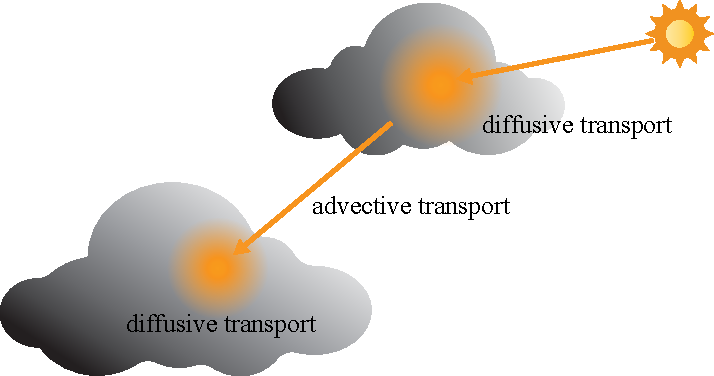
\includegraphics[width=0.55\textwidth]{06_fld/figures/fig_transport_regimes_scene.pdf}
%\missingfigure{show image with isotropic distribution, streaming limit distribution and inbetween forms}
\caption{Radiative transfer in typical scenes contains a mix of transport regimes as shown in this figure. Diffuse transport in dense media with high absorption and advective transport in thin media. The idea behind the Variable Eddington Factor is to express radiative transfer as a mix between those two extreme transport modes.}
\label{fig:fld_vef_advection_diffusion2}
\end{figure}

The Variable Eddington Factor form of $T$ is derived by considering a principal direction of transport, given by the vector $\vec{n}$ of unit length. An important assumption is that the radiance distribution will be radially symmetric around this direction. This means, that the value of $\hat{L}$ will be invariant to a rotation about axis $\vec{n}$. It follows, that its first and second moment $\hat{L}_1$ and $\hat{L}_2$ will also be invariant to rotation about $\vec{n}$. If one approximates $\hat{L}_2$ using the Eddington tensor $T$ with $\hat{L}_2\approx T\phi$, it can be concluded that $\vec{n}$ will be an eigenvector of $T$ with eigenvalue $\chi$:
\begin{align*}
T\vec{n} = \chi\vec{n}
\end{align*}
%\TD{explain/give reference why eigenvectors need to sum up to one}
The plane perpendicular to $\vec{n}$ is an eigenspace of $T$. By requiring that all eigenvalues sum up to one, the eigenvalues of the two eigenvectors spanning that plane by distributing the remaining eigenvalue $1-\chi$ evenly between both is expressed as:
\begin{align}
\frac{1}{2}\left(1-\chi\right)\mathbf{I}
\label{eq:iso_var_T_isoterm}
\end{align}
From the free streaming limit case (section~\ref{sec:fld_streaming_limit_approximation}), it is known that $\chi=1$, when the radiance distribution becomes a delta distribution (equation~\ref{eq:zero_moment_Lhat} and~\ref{eq:first_moment_Lhat}). In that case, the eigenvalues associated with the eigenvectors perpendicular to $\vec{n}$ become zero and the term above vanishes.

Tensor diagonalization allows to explicitly add the eigenvector $\vec{n}$ by adding the matrix $\vec{n}_i\vec{n}_j$ (with $\vec{n}$ being of unit length). The scaling of its coefficients is found by considering that the term in equation~\ref{eq:iso_var_T_isoterm} introduces three eigenvectors. The sum of their eigenvalues will be $3/2(1-\chi)$. Since eigenvalues of the final tensor $T$ need to add up to one, the eigenvalue associated with the matrix $\vec{n}_i\vec{n}_j$ will be $\left(1- \frac{3}{2}\left(1 - \chi\right)\right)$. This results in the following form for $T$:
\begin{align}
T &= \frac{1}{2}\left(1-\chi\right)\mathbf{I} + \left(1- \frac{3}{2}\left(1 - \chi\right)\right) \vec{n}\otimes\vec{n}
\nonumber
\\
&= \frac{1}{2}\left(1-\chi\right)\mathbf{I} + \frac{1}{2}\left(3\chi-1\right) \vec{n}\otimes\vec{n}
\label{eq:iso_var_T}
\end{align}
This form of $T$ is called the Variable Eddington Tensor (VET). It can be understood as an \emph{interpolation} between an isotropic distribution tensor ($1/3\mathbf{I}$) and a delta distribution tensor ($\vec{n}_i\vec{n}_j$). The variable $1/3 \le \chi \le 1$ is the interpolation variable and is called the Eddington factor (VEF). Theories, which respect this structure of the Eddington tensor are referred to as theories under the variable Eddington factor formalism (VEF-formalism).

If $\chi=1/3$, then equation~\ref{eq:iso_var_T} will result in the isotropic distribution tensor, which is the base assumption for classical diffusion:
\begin{align}
\frac{1}{2}\frac{2}{3}\mathbf{I} + \frac{1}{2}\left(\frac{3}{3}-1\right) \vec{n}\otimes\vec{n}
=\frac{1}{3}\mathbf{I} + 0\vec{n}\otimes\vec{n} = \frac{1}{3}\mathbf{I}
\end{align}
For $\chi=1$, equation~\ref{eq:iso_var_T} produces the Eddington tensor, which was derived for the pure streaming limit distribution, where all light comes from a singular direction:
\begin{align}
\frac{1}{2}0\mathbf{I} + \vec{n}\otimes\vec{n}
= \vec{n}\otimes\vec{n}
\end{align}
The Eddington factor $\chi$ can also be interpreted as a measure of anisotropy of the radiance distribution $\widehat{L}$ with respect to direction $\vec{n}$. It can be expressed in terms of the radiance distribution by the squared mean cosine (given by Levermore~\cite{Levermore84}):
\begin{align}
\chi &= \int_{S^2}{ \left(\omega\cdot\vec{n}\right)^2\hat{L}\left(\vec{x}, \omega\right)\ud\omega}
\label{eq:iso_var_chi}
\end{align}
With the variable Eddington factor approach, only a function for the interpolation variable $\chi$ (the actual Eddington factor) needs to be identified. This function should have $1/3$ and $1$ as its limits. With such an interpolation function, the limit transport cases (diffusion and free streaming) will be a subset of any theory, which adheres to the variable Eddington factor concept.

The Eddington factor framework, sets up the Eddington factor and the limits of its parameterization, $\chi$. The specific expression for this factor is not defined and it is clear that there are many options for the function $\chi$, which respect the given function limits. This is why there is such a rich variety of theories in other domains, which all propose their own version of that interpolation function. Some of them are ad-hoc schemes (Bowers et al.~\cite{Bowers82}, Kershaw~\cite{Kershaw76} and Larsen et al.~\cite{Larsen74}), which are derived from heuristics, while others have a clear connection to transport theory (Levermore at al.~\cite{Levermore81}) or are derived from entropy theory (Minerbo~\cite{Minerbo78}).

The general strategy for all these different variable Eddington factor theories is:
\begin{enumerate}
\item Find a model or theory, from which a certain radially symmetric form of the radiance distribution $\hat{L}$ about the normalized flux-vector$\vec{E}/\phi$ can be found or justified.
\item Then derive an expression for $\chi(\vec{E}/\phi)$ from the model for $\hat{L}$, which can be used to construct $T$. Further assumptions are applied, to be able to express $\vec{E}$ in terms of $\nabla\phi$. This is required in order to not have $T$ depend on the flux-vector directly as it still needs to be possible to resolve equation~\ref{eq:me_first_resolved_E} for the flux-vector.
\end{enumerate}

In this thesis, results for different theories have been presented and implemented, but only flux-limited diffusion from Levermore et. al~\cite{Levermore81} was discussed, since it is the most popular and also has the strongest connection to transport theory. Discussing all other theories is beyond the scope of this thesis and also not really necessary, as it is shown in section~\ref{sec:fld_results} that the particular choice of theory is not of significant importance for applications in computer graphics.
\section{Flux-limiters}
\label{sec:fld_vef_factors}

Levermore et. al~\cite{Levermore81} construct their theory by starting from the time-dependent form of the radiative transfer equation. They further assume a constant phase function $f_p=1/(4\pi)$:
\begin{align}
\label{eq:iso_var_fld_rte}
\frac{1}{c}\frac{\partial (\phi\hat{L})}{\partial t} + \left(\vec{\omega}\cdot\nabla\right)(\phi\hat{L})&=-\sigma_t\phi\hat{L} + \frac{1}{4\pi}\sigma_s\phi + Q
\end{align}
After applying the moment expansion, for the first moment equations are as follows:
\begin{align}
\label{eq:iso_var_fld_rte_zero}
\frac{1}{c}\frac{\partial \phi}{\partial t} + \nabla\vec{E} &= -\sigma_a\phi + Q_0
\end{align}
As a next step, equation~\ref{eq:iso_var_fld_rte_zero} is resolved for $\partial \phi/\partial t$ on the left hand side and used to substitute $\partial\phi/\partial t$ in equation~\ref{eq:iso_var_fld_rte} (after applying the product rule to the time derivative term). By further assuming the absence of self-emission ($Q=0$) and that the space and time derivatives of the radiance distribution $\hat{L}$ can be neglected, the result is:
\begin{align}
\label{eq:iso_var_fld_eliminated_time}
\left( \left(\vec{\omega}\cdot\nabla\right)\phi -\vec{f}\cdot\nabla\phi + \sigma_t'\phi\right)\hat{L} = \frac{1}{4\pi}\sigma_t'\phi
\end{align}
Solving equation~\ref{eq:iso_var_fld_eliminated_time} for $\hat{L}$ gives:
\begin{align}
\label{eq:iso_var_fld_Lhat}
\hat{L} = \frac{1}{4\pi}\frac{1}{1+\widehat{\vec{E}}\cdot\vec{R}-\vec{\omega}\cdot\vec{R}}
\end{align}
with
\begin{align}
\label{eq:iso_var_fld_R}
\vec{R} = -\frac{\nabla\phi}{\sigma_t'\phi}
\end{align}
The definition of the flux-vector in equation~\ref{eq:second_moment_iso3} is used, which was derived in section~\ref{sec:fld_streaming_limit_approximation}:
\begin{align}
\widehat{\vec{E}} = \frac{\vec{E}}{\phi}= T\vec{R}
\label{eq:iso_var_fld_normalized_flux}
\end{align}

Following the same argument about the radial symmetry of $\hat{L}$ and its relation to the flux-vector and eigenvectors of $T$, $T$ is replaced with a proportionality function $\lambda(R)$, where $R=\norm{\vec{R}}$:
\begin{align}
\widehat{\vec{E}} = \lambda(R)\vec{R}
\label{eq:iso_var_fld_relation_normalized_flux_R}
\end{align}

Using this in equation~\ref{eq:iso_var_fld_Lhat} gives:
\begin{align}
\label{eq:iso_var_fld_Lhat_R}
\hat{L} = \frac{1}{4\pi}\frac{1}{1+\lambda(R)R^2-\vec{\omega}\cdot\vec{R}}
\end{align}

By enforcing that $\hat{L}$ integrates to one over the solid angle of the unit sphere, the following expression for $\lambda(R)$ can be derived:
\begin{align}
\label{eq:iso_var_fld_lambdaR}
\lambda(R) = \frac{1}{R}\left(\mathbf{\operatorname{coth}}R - \frac{1}{R}\right)
\end{align}

Using this result and equation~\ref{eq:iso_var_fld_relation_normalized_flux_R}, gives the following expression for the flux vector:
\begin{align}
\label{eq:iso_var_fld_fluxvector}
\vec{E} = \widehat{\vec{E}}\phi=-\frac{1}{\sigma_t'}\lambda(R)\nabla\phi
\end{align}

Inserting this into the zero moment equation (equation~\ref{eq:me_zero}) gives the flux-limited diffusion equation, a diffusion-type equation of the following form:
\begin{align}
\label{eq:iso_var_fld_final}
\nabla\left( \underbrace{-\frac{1}{\sigma_t'}\lambda(R)}_{D_F}\nabla\phi\right) &= -\sigma_a\phi + Q_0
\end{align}

The flux-limited diffusion coefficient $D_F$ is non-linear and therefore turns the zero moment equation into a non-linear diffusion equation. $\lambda(R)$ is called the flux-limiter. In the diffusion limit, $R$ approaches zero and the flux-limiter approaches $\lambda(R)=1/3$, which will turn equation~\ref{eq:iso_var_fld_final} into the classical diffusion equation for isotropic media.
\begin{align}
\lim_{R\rightarrow 0 }D_F =-\frac{1}{3\sigma_t'}
\implies
\nabla
\left(
-\frac{1}{3\sigma_t'\left(\vec{x}\right)}
\nabla \phi\left(\vec{x}\right)
\right)
=
-\phi(\vec{x})\sigma_a(\vec{x})
+Q_0\left(\vec{x}\right)
\end{align}
In the transport limit, $R$ will approach infinity and the diffusion coefficient will cause the equation to become an advection equation as seen in the delta radiance distribution case (equation~\ref{eq:iso_delta_advection_equation}):
\begin{align}
\lim_{R\rightarrow\infty }D_F =-\frac{\phi}{\norm{\nabla\phi}}
\implies
\nabla
\left(
-\phi\frac{\nabla\phi\left(\vec{x}\right)}{\norm{\nabla\phi}}
\right)
=
-\phi(\vec{x})\sigma_a(\vec{x})
+Q_0\left(\vec{x}\right)
\end{align}
It can be seen that the flux-limited diffusion coefficient will normalize the fluence gradient $\nabla\phi$ to unit length and scale with the total power $\phi$. Flux-limited diffusion not only suppresses the flux in the free streaming transport regime, it also saturates it at the appropriate value to ensure correct free propagation (at the level of the approximation).

The flux-limiter introduced by Levermore et al.~\cite{Levermore81} was shown to relate to the variable Eddington factor approach in a seperate study (\cite{Whalen82, Levermore84}) to be:
\begin{align}
\label{eq:iso_var_fld_vef}
\chi = \lambda(R) + \lambda(R)^2R^2
\end{align}
As mentioned in the previous section, the theory sets up the limits, which flux-limiters have to respect. This allows different models and theories to find and justify particular choices of flux-limiters. Table~\ref{tbl:flux-limiters} presents the most prominent flux-limiters.
\begin{table}[h]
\center
\caption{Various prominent flux-limiters which all respect the Eddington factor limits and represent different flux-limited diffusion theories.}
\begin{tabular}{ l l }
\hline\hline
 Flux-limiter & $\lambda\left(R\right)$ \\ 
\hline
 sum~\cite{Bowers82} & $(3+R)^{-1}$ \\
 max~\cite{Bowers82} & $\mbox{max}(3, R)^{-1}$ \\
 Kershaw~\cite{Kershaw76} & $2(3+\sqrt{9 + 4R^2}\,)^{-1}$ \\
 Larsen-$n$~\cite{Larsen74} & $(3^n + R^n)^{-\frac{1}{n}}$ \\
 Levermore-Pomraning~\cite{Levermore81} & $\frac{1}{R} \left(\coth(R)-\frac{1}{R}\right)$    
\end{tabular}
\label{tbl:flux-limiters}
\end{table}

\begin{figure}[h]
\centering
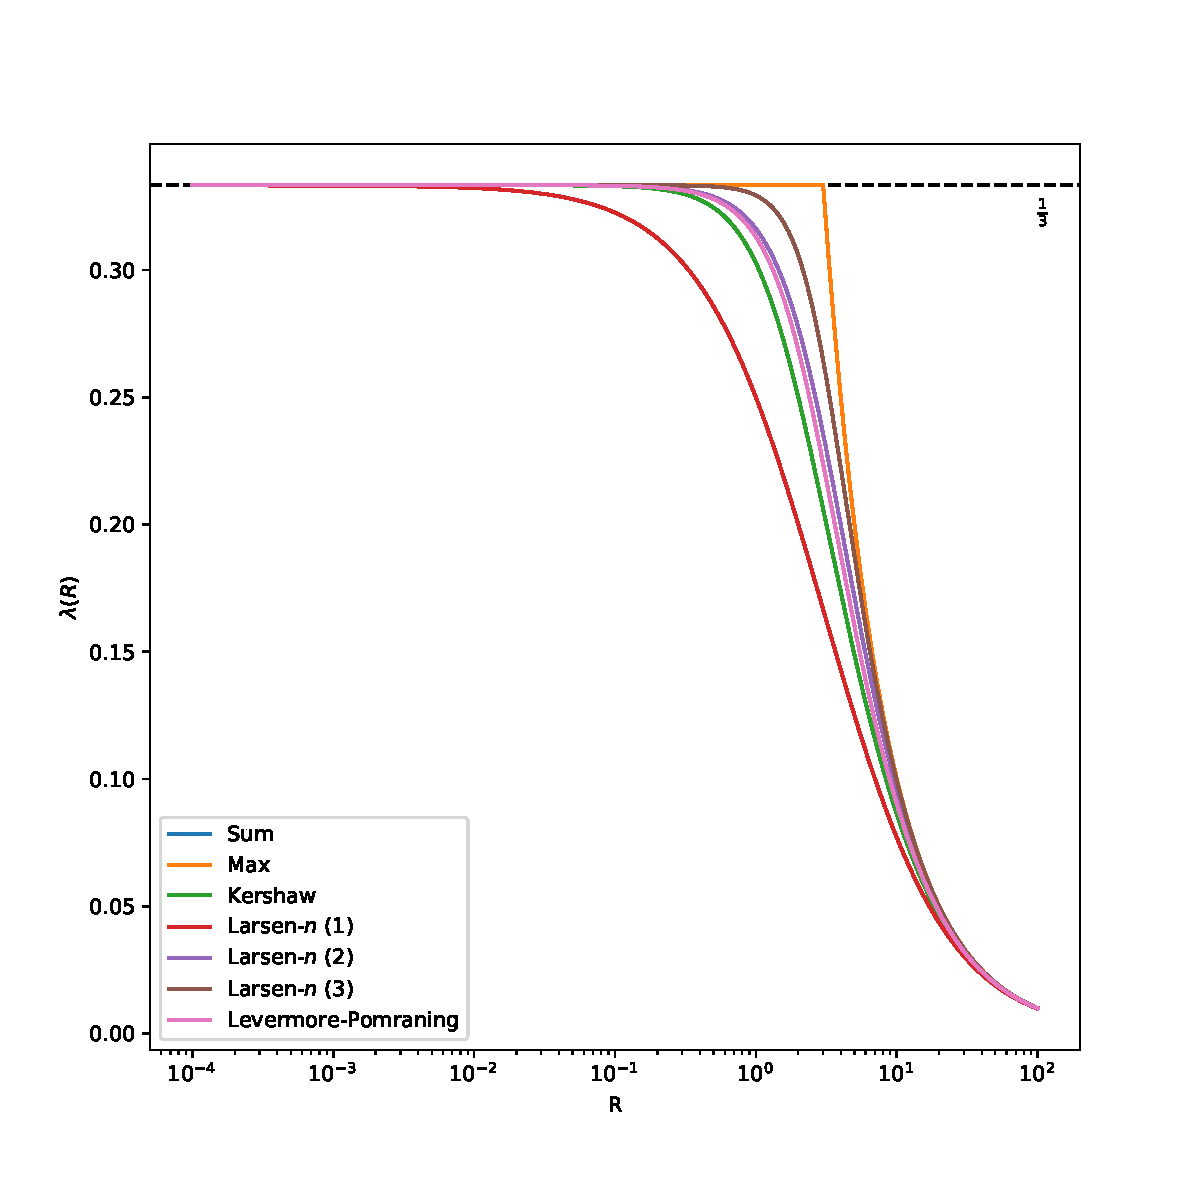
\includegraphics[width=0.65\textwidth]{06_fld/figures/plot_flux_limiters.pdf}
\caption{Plot of the various flux-limiters shown in table~\ref{tbl:flux-limiters}.}
\label{fig:flux-limiters}
\end{figure}
%
%\missingfigure{flux-limiters graphs}

In this section a non-linear form of the diffusion equation is derived which respects the flux-limit constraint. The following section will present a novel solver, which solves flux-limited diffusion on a finite difference grid over a given domain.



\section{Non-Linear Gauss-Seidel Solver with Successive Overrelaxation}
\label{sec:fld_solver}

\section{Results}
\label{sec:fld_results}

\TD{mention publication}
\TD{mention application in elementacular}
\chapter{Conclusion}
%
\label{sec:conclusion}

The main focus in contemporary rendering research are non-deterministic methods for light transport simulation. Boosting the convergence of these methods is the main thrust of todays efforts in research groups world wide. In particular path-guiding based approaches are becoming increasingly popular as they have shown to improve non-deterministic methods significantly by using a global approximation of the radiance field to allow better informed decisions during stochastic sampling.

At the same time a shift in compute hardware manufacturing from clock frequency growth to growth in core count with the next generation of multi-core and many-core hardware on the horizon is seen. High performance computing centers, which have large scale multi-core parallelization at the core of their business, are opening up and undergo a transformation towards becoming providers for public massive multi-core cloud computing. Developing algorithms which cater to the characteristics of this new hardware is deemed as one of the major challenges in future rendering research.

Both trends, path-guiding and multi-core hardware, are the main motivation for revisiting deterministic methods for light transport simulation, which have received little attention in the past years. In particular there is a large body of research related to deterministic methods in fields such as astrophysics or nuclear sciences. Going through that research and adopting it for application in computer graphics has been fruitful in the past and is the main spirit behind the research done as part of this thesis. The three chapters on the $P_N$-method (chapter~\ref{sec:pnmethod}), the diffusion approximation (chapter~\ref{sec:diffusion_approximation}) and flux-limited diffusion (chapter~\ref{sec:fld}) constitute and reflect the majority of the results.

The first major contribution of this thesis to the field of computer graphics is the full introduction of $P_N$-theory to the field. While the theory has been around and used for a long time in astrophysics and nuclear sciences, it has never been applied to the problem of rendering in computer graphics. In that regard the contribution of this thesis is to serve as a bridge to better understand related research from other fields. The $P_N$-theory is dense and unwieldy to work with. This thesis revists the theory and presents it to the audience in modern graphics research. A side product of this is a new and very concise form of the real-valued $P_N$-equations.

While the theory has been existing in other fields and was only established as new to the graphics domain, the method for solving the $P_N$-equations, which was developed as part of this thesis, is a novel contribution standing on its own and resulted in the publication by Koerner et al.~\cite{Koerner18}. The positive reviews and encouraging comments from the graphics community after the corresponding conference talk reconfirmed that this contribution closes an important gap in the graphics field.

The diffusion approximation is derived from $P_N$-theory by truncating the spherical harmonics expansion after the first moment and is therefore a deterministic method for light transport simulation based on the spherical harmonics expansion of the radiative transfer equation. It plays a very important role for many rendering techniques and was applied to many different problems in realtime and production rendering. This is why diffusion theory has been included in its own chapter in this thesis. Here, the contribution to graphics by this thesis lies primarily in showing the connection between the moment expansion and the more popular spherical harmonics expansio. This allows a clear derivation of the classical well known diffusion equation and, more importantly, lays the foundation to the main contribution of this thesis in the subsequent chapter.

The second major contribution in this thesis is the introduction of flux-limited diffusion in chapter~\ref{sec:fld} to the field of computer graphics. With the $P_N$-method, flux-limited diffusion has been invented in the astrophysics domain and also became popular in nuclear sciences and medical sciences. However, it has never been applied to the problem of rendering in computer graphics before. Firstly, the theory is derived as a consequence of addressing deficiencies in diffusion theory. Therefore, the theory section builts up on the theoretical foundations layed out in previous chapters. In addition to exposing the theory to the graphics community the contribution from this chapter is also a new method for solving the flux-limited diffusion equation, which allows for practical rendering applications. These contributions have been published by Koerner et al.~\cite{Koerner14}. In particular the solver has been adopted in the industry (see figure~\ref{fig:fld_conclusion_elementacular_1}).
\begin{figure}[h]
\centering
%\missingfigure{use of FLD in elementacular}
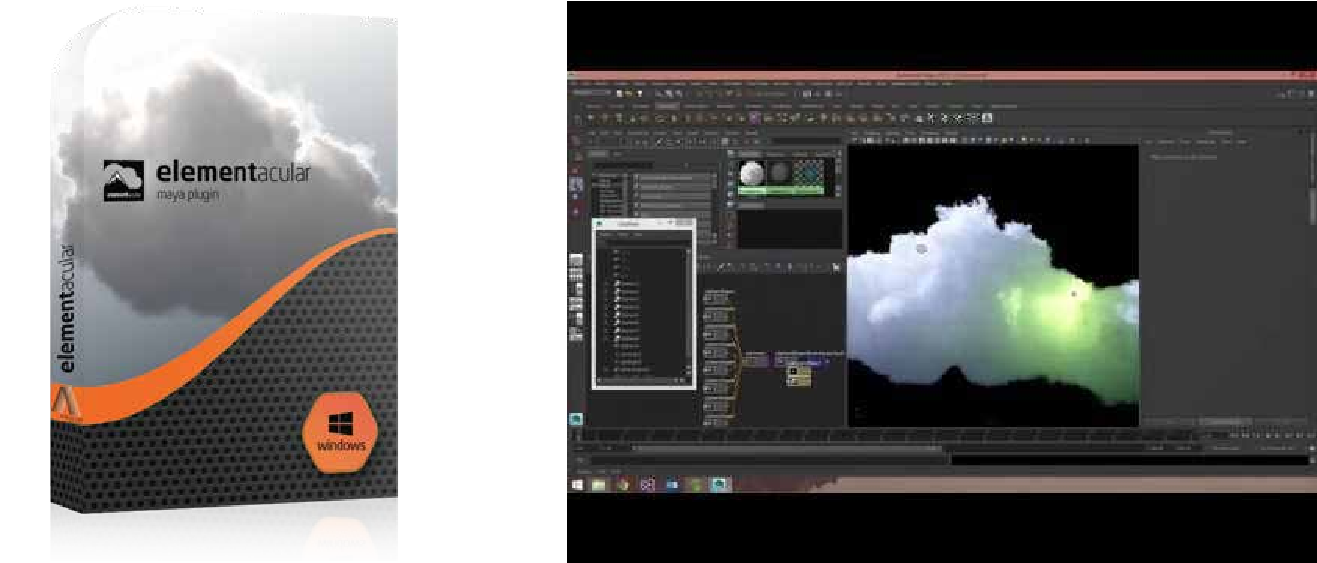
\includegraphics[width=0.95\textwidth]{07_conclusion/figures/fig_elementacular.pdf}
\caption{Flux-limited diffusion is used to compute multiple scattering in Elementacular\protect\footnotemark, a commercial plugin for interactive cloud modelling. Due to the incremental nature of interactive edits, the result from previous frames is a great initial solution for the solver, which then only needs a few iterations to resolve.}
\label{fig:fld_conclusion_elementacular_1}
\end{figure}


With $P_N$-theory, diffusion and flux-limited diffusion, this thesis gives a comprehensive treatment of the domain of deterministic methods that are based on the spherical harmonics expansion of the radiative transfer equation. For every chapter the theory is derived and a solver is being devised for solving the corresponding equations. This thesis becomes a relevant important document for understanding the methods and their application in practical applications.\footnotetext{\url{http://elementacular.com} (date of access: 10/02/2019)} 

\subsubsection*{Outlook}

However, while being comprehensive, the coverage of spherical harmonics based methods for light transport simulation in this thesis is neither exhaustive nor complete. Although it has a long history, the field is still being actively researched and advanced primarily by the nuclear science community.

The $P_N$-theory provides a solid framework for discretizing the radiative transfer equation in angular domain. However, for practical applications concerned with stead-state problems, the $P_N$-method suffers from having to solve very large linear systems if the truncation order is increased. This makes it unviable for real world applications. In addition the theory and all its derivatives, such as the diffusion approximation and flux-limited diffusion, suffer from the presence of vacuum regions in the problem domain. More specifically, all three methods will not be able to converge for these problems. This is a major issue for application in graphics, where vacuum regions are ubiquitous.

A direction for future research that has not been explored fully yet is to devise a multigrid method for solving the large coupled system of $P_N$-equations. Such a multigrid scheme could make the method more competitive in comparison to other approaches.

The introduction of the diffusion approximation has led to a variety of methods in computer graphics and a similar development can be envisioned for the $P_N$-method. The extension to finite-elements discretization or handling of more complex boundary conditions could allow the application of the $P_N$-method to problems such as subsurface scattering.

To deal with the vacuum problem one direction for future research needs to be the evaluation of the various variations of the $P_N$-method, which have been proposed in other domains, such as nuclear sciences. Evaluating these variations was one idea behind the design of the solver in chapter~\ref{sec:pnmethod}, as all the variations are presented as a coupled system of partial differential equations which could be all fed as input to the solver developed as part of this chapter.

There are no obivous open questions regarding the diffusion approximation. This comes at no surprise since diffusion has been introduced to graphics a long time ago and received a lot of attention from graphics researchers throughout the years. Its traits are known and well studied.

Flux-limited diffusion offers a great balance between computational efficiency and accuracy, therefore has seen some interest for industry application recently. As its linear counterpart, the non-linear Gauss-Seidel solver does not scale well with the resolution of the finite difference grid. Here, it seems like a promising avenue to investigate non-linear multigrid solvers. Being able to apply flux-limited diffusion to much larger problem sizes could significantly broaden its applicability.

Another interesting direction could be to extend flux-limited diffusion or even the $P_N$-theory in general to anisotropic media. All literature on $P_N$-theory is based on isotropic media and deriving a $P_N$-theory for anisotropic media could open up directions for new deterministic methods in this field. While anisotropic media appears to play a minor role in graphics at the moment, some research, such as the work by Dupuy et al.~\cite{Dupuy16}, indicates that anisotropic media might be an important building block for bridging the divide between surface rendering (rendering equation) and volume rendering (radiative transfer).

The place of deterministic methods in rendering is uncertain due to their complexities, such as discretization bias, convergence issues and boundary conditions. Particularly, deterministic methods lack the appeal of conceptional simplicity that non-deterministic methods, such as Monte-Carlo, have. This not only prevents their adoption in the industry, but also makes them unattractive as a research subject as such. This thesis represents a significant effort to fill prominent knowledge gaps and demonstrate that deterministic methods and spherical harmonics based techniques in particular can be easily understood and provide very powerful tools in rendering.











%\include{03_Background/Background}
%\include{04_Related_Work/Related_Work}
%\include{05_HdM-HDR-2014/HdM-HDR-2014}
%\include{06_ICaCb/ICaCb}
%\include{07_Reshaping/Reshaping}
%\include{08_Conclusion/Conclusion}

%
% Jan Fix for weird LaTex behaviour:
%\fancyhead[LO]{\bfseries Publications} 
%\fancyhead[RE]{\bfseries Publications}
%\include{01_Preamble/Publications} 
%\cleardoublepage
%
% Jan Fix for weird LaTex behaviour:
%\fancyhead[LO]{\bfseries Bibliography} 
%\fancyhead[RE]{\bfseries Bibliography}
%\addcontentsline{toc}{chapter}{Bibliography}
%
%%GATHER{Bibliography.bib}   % For Gather Purpose Only (v useful in winedt)
%
%\singlespacing
%
%%\bibliographystyle{ACM-Reference-Format-Journals} % {abbrvnatjan}% {abbrvnat} % abbrvnat
\bibliographystyle{abbrvnat}
%%\bibliographystyle{ieeetr} % Jan 2016/05 better numbering but loosing URLs
%
%% \emergencystretch 1.5em % Should split URLS
%%\interlinepenalty=10000 % should remove splitting of items over pages
\bibliography{bibliography}

\cleardoublepage
%
\onehalfspacing
\phantomsection
\renewcommand{\theHchapter}{\appendixname.\thechapter} % Fixe pdf Link Problem
% Jan Fix for weird LaTex behaviour:
\fancyhead[LO]{\bfseries Appendix} 
\fancyhead[RE]{\bfseries Appendix}
\appendix
%
\phantomsection
\chapter{Appendix: Derivation of Real-valued $P_N$-equation Terms}
\label{app:rpn}


We later will have to apply identities and properties for the complex-valued SH basis functions and therefore need to expand the real-valued basis function in $\hat{L}$. The real-valued basis function is different depending on $m$ and therefore gives different expansions for the sign of $m$:
\begin{align}
\hat{L}\left(\vec{x}, \vec{\omega}\right)
=&
\left\{
\begin{array}{lr}
\sum_{l,m}L^{l,m}\left(\vec{x}\right)\frac{\iu}{\sqrt{2}}\left(\SHBC^{l,m}-\left(-1\right)^m\SHBC^{l,-m}\right), & \text{for } m < 0\\
\sum_{l,m}L^{l,m}\left(\vec{x}\right)\SHBC^{l,m}, & \text{for } m = 0\\
\sum_{l,m}L^{l,m}\left(\vec{x}\right)\frac{1}{\sqrt{2}}\left(\SHBC^{l,-m}-\left(-1\right)^m\SHBC^{l,m}\right), & \text{for } m > 0
\end{array}
\right.
\nonumber\\
=&
\left\{
\begin{array}{lr}
\sum_{l}\sum_{m=-l}^{-1}L^{l,m}\left(\vec{x}\right)\frac{\iu}{\sqrt{2}}\left(\SHBC^{l,m}-\left(-1\right)^m\SHBC^{l,-m}\right), & \text{for } m < 0\\
L^{l,0}\left(\vec{x}\right)\SHBC^{l,0}, & \text{for } m = 0\\
\sum_{l}\sum_{m=1}^{l}L^{l,m}\left(\vec{x}\right)\frac{1}{\sqrt{2}}\left(\SHBC^{l,-m}-\left(-1\right)^m\SHBC^{l,m}\right), & \text{for } m > 0
\end{array}
\right.
\nonumber\\
=&
\sum_{l=0}^{N}
\left(
\sum_{m=-l}^{-1}
{
L^{{l,m}}\left (\vec{x} \right )\left(\frac{i}{\sqrt{2}}\SHBC^{l, m}(\vec{\omega} )-\frac{i}{\sqrt{2}}\left({-1}\right)^{m}\SHBC^{l, -m}(\vec{\omega} )\right)
}
\right.
\nonumber\\
&
+L^{l,0}\left (\vec{x} \right )\SHBC^{l, 0}(\vec{\omega} )
\nonumber\\
&
+
\left.
\sum_{m=1}^{l}
{
L^{{l,m}}\left (\vec{x} \right )\left(\frac{1}{\sqrt{2}}\SHBC^{l, -m}(\vec{\omega} )+\frac{1}{\sqrt{2}}\left({-1}\right)^{m}\SHBC^{l, m}(\vec{\omega} )\right)
}
\right)
\nonumber\\=&
\frac{i}{\sqrt{2}}\left(\sum_{l=0}^{N}{\sum_{m=-l}^{-1}{L^{{l,m}}\left (\vec{x} \right )\SHBC^{l, m}(\vec{\omega} )}}\right)
-\frac{i}{\sqrt{2}}\left(\sum_{l=0}^{N}{\sum_{m=-l}^{-1}{L^{{l,m}}\left (\vec{x} \right )\left({-1}\right)^{m}\SHBC^{l, -m}(\vec{\omega} )}}\right)
\nonumber\\&
+\sum_{l=0}^{N}{L^{{l,0}}\left (\vec{x} \right )\SHBC^{l, 0}(\vec{\omega} )}
\nonumber\\&
+\frac{1}{\sqrt{2}}\left(\sum_{l=0}^{N}{\sum_{m=1}^{l}{L^{{l,m}}\left (\vec{x} \right )\SHBC^{l, -m}(\vec{\omega} )}}\right)
+\frac{1}{\sqrt{2}}\left(\sum_{l=0}^{N}{\sum_{m=1}^{l}{L^{{l,m}}\left (\vec{x} \right )\left({-1}\right)^{m}\SHBC^{l, m}(\vec{\omega} )}}\right)
\end{align}

The transport term of the RTE is given as
\begin{align}
(\vec{\omega}\cdot\nabla)L(\vec{x}, \vec{\omega})
=
\vec{\omega}_{x}\partial_xL\left (\vec{x} ,\vec{\omega} \right )+\vec{\omega}_{y}\partial_yL\left (\vec{x} ,\vec{\omega} \right )+\vec{\omega}_{z}\partial_zL\left (\vec{x} ,\vec{\omega} \right )
\label{eq:real_transport_term}
\end{align}

To improve readability, we first project the term into SH by multiplying with the conjugate complex of the Sh basis, and replace $L$ by its Sh expansion afterwards. This order was reversed, when we derived the complex-valued $P_N$-equation in section~\ref{sec:pn_cvalued}.

We now multiply equation~\ref{eq:real_transport_term} with the real-valued SH basis and integrate over solid angle. However, the SH basis is different for $m'<0$, $m'=0$ and $m'>0$, and therefore will give us different $P_N$-equations depending on $m'$. We will go through the derivation in detail for the $m'<0$ case and give the results for the other cases at the end.

Multiplying the expanded transport term with the SH basis for $m'<0$ and integrating over solid angle gives:
\begin{align*}
&\int{\left(\frac{-i}{\sqrt{2}}\overline{Y^{l', m'}}(\vec{\omega} )-\frac{-i}{\sqrt{2}}\left({-1}\right)^{m'}\overline{Y^{l', -m'}}(\vec{\omega} )\right)\left(\vec{\omega}_{x}\partial_xL\left (\vec{x} ,\vec{\omega} \right )+\vec{\omega}_{y}\partial_yL\left (\vec{x} ,\vec{\omega} \right )+\vec{\omega}_{z}\partial_zL\left (\vec{x} ,\vec{\omega} \right )\right)\ud\vec{\omega}}
\\
=&
\int-\frac{i}{\sqrt{2}}\overline{Y^{l', m'}}(\vec{\omega} )\vec{\omega}_{x}\partial_xL\left (\vec{x} ,\vec{\omega} \right )-\frac{i}{\sqrt{2}}\overline{Y^{l', m'}}(\vec{\omega} )\vec{\omega}_{y}\partial_yL\left (\vec{x} ,\vec{\omega} \right )-\frac{i}{\sqrt{2}}\overline{Y^{l', m'}}(\vec{\omega} )\vec{\omega}_{z}\partial_zL\left (\vec{x} ,\vec{\omega} \right )
\\&
+\frac{i}{\sqrt{2}}\left({-1}\right)^{m'}\overline{Y^{l', -m'}}(\vec{\omega} )\vec{\omega}_{x}\partial_xL\left (\vec{x} ,\vec{\omega} \right )+\frac{i}{\sqrt{2}}\left({-1}\right)^{m'}\overline{Y^{l', -m'}}(\vec{\omega} )\vec{\omega}_{y}\partial_yL\left (\vec{x} ,\vec{\omega} \right )
\\&
+\frac{i}{\sqrt{2}}\left({-1}\right)^{m'}\overline{Y^{l', -m'}}(\vec{\omega} )\vec{\omega}_{z}\partial_zL\left (\vec{x} ,\vec{\omega} \right )\ud\vec{\omega}
\end{align*}

After expanding the integrand and splitting the integral, we apply the recursive relation from equation~\ref{eq:recursive_relation} to get:
\begin{align*}
&
\frac{i}{\sqrt{2}}\frac{1}{2}c^{{l'-1,m'-1}}\int{\partial_xL\left (\vec{x} ,\vec{\omega} \right )\overline{Y^{l'-1, m'-1}}(\vec{\omega} )\ud\vec{\omega}}
-\frac{i}{\sqrt{2}}\frac{1}{2}d^{{l'+1,m'-1}}\int{\partial_xL\left (\vec{x} ,\vec{\omega} \right )\overline{Y^{l'+1, m'-1}}(\vec{\omega} )\ud\vec{\omega}}
\\&
-\frac{i}{\sqrt{2}}\frac{1}{2}e^{{l'-1,m'+1}}\int{\partial_xL\left (\vec{x} ,\vec{\omega} \right )\overline{Y^{l'-1, m'+1}}(\vec{\omega} )\ud\vec{\omega}}
+\frac{i}{\sqrt{2}}\frac{1}{2}f^{{l'+1,m'+1}}\int{\partial_xL\left (\vec{x} ,\vec{\omega} \right )\overline{Y^{l'+1, m'+1}}(\vec{\omega} )\ud\vec{\omega}}
\\&
-\frac{i}{\sqrt{2}}\frac{i}{2}c^{{l'-1,m'-1}}\int{\partial_yL\left (\vec{x} ,\vec{\omega} \right )\overline{Y^{l'-1, m'-1}}(\vec{\omega} )\ud\vec{\omega}}
+\frac{i}{\sqrt{2}}\frac{i}{2}d^{{l'+1,m'-1}}\int{\partial_yL\left (\vec{x} ,\vec{\omega} \right )\overline{Y^{l'+1, m'-1}}(\vec{\omega} )\ud\vec{\omega}}
\\&
-\frac{i}{\sqrt{2}}\frac{i}{2}e^{{l'-1,m'+1}}\int{\partial_yL\left (\vec{x} ,\vec{\omega} \right )\overline{Y^{l'-1, m'+1}}(\vec{\omega} )\ud\vec{\omega}}
+\frac{i}{\sqrt{2}}\frac{i}{2}f^{{l'+1,m'+1}}\int{\partial_yL\left (\vec{x} ,\vec{\omega} \right )\overline{Y^{l'+1, m'+1}}(\vec{\omega} )\ud\vec{\omega}}
\\&
-\frac{i}{\sqrt{2}}a^{{l'-1,m'}}\int{\partial_zL\left (\vec{x} ,\vec{\omega} \right )\overline{Y^{l'-1, m'}}(\vec{\omega} )\ud\vec{\omega}}
-\frac{i}{\sqrt{2}}b^{{l'+1,m'}}\int{\partial_zL\left (\vec{x} ,\vec{\omega} \right )\overline{Y^{l'+1, m'}}(\vec{\omega} )\ud\vec{\omega}}
\\&
-\frac{i}{\sqrt{2}}\left({-1}\right)^{m'}\frac{1}{2}c^{{l'-1,-m'-1}}\int{\partial_xL\left (\vec{x} ,\vec{\omega} \right )\overline{Y^{l'-1, -m'-1}}(\vec{\omega} )\ud\vec{\omega}}
\\&
+\frac{i}{\sqrt{2}}\left({-1}\right)^{m'}\frac{1}{2}d^{{l'+1,-m'-1}}\int{\partial_xL\left (\vec{x} ,\vec{\omega} \right )\overline{Y^{l'+1, -m'-1}}(\vec{\omega} )\ud\vec{\omega}}
\\&
+\frac{i}{\sqrt{2}}\left({-1}\right)^{m'}\frac{1}{2}e^{{l'-1,-m'+1}}\int{\partial_xL\left (\vec{x} ,\vec{\omega} \right )\overline{Y^{l'-1, -m'+1}}(\vec{\omega} )\ud\vec{\omega}}
\\&
-\frac{i}{\sqrt{2}}\left({-1}\right)^{m'}\frac{1}{2}f^{{l'+1,-m'+1}}\int{\partial_xL\left (\vec{x} ,\vec{\omega} \right )\overline{Y^{l'+1, -m'+1}}(\vec{\omega} )\ud\vec{\omega}}
\\&
+\frac{i}{\sqrt{2}}\left({-1}\right)^{m'}\frac{i}{2}c^{{l'-1,-m'-1}}\int{\partial_yL\left (\vec{x} ,\vec{\omega} \right )\overline{Y^{l'-1, -m'-1}}(\vec{\omega} )\ud\vec{\omega}}
\\&
-\frac{i}{\sqrt{2}}\left({-1}\right)^{m'}\frac{i}{2}d^{{l'+1,-m'-1}}\int{\partial_yL\left (\vec{x} ,\vec{\omega} \right )\overline{Y^{l'+1, -m'-1}}(\vec{\omega} )\ud\vec{\omega}}
\\&
+\frac{i}{\sqrt{2}}\left({-1}\right)^{m'}\frac{i}{2}e^{{l'-1,-m'+1}}\int{\partial_yL\left (\vec{x} ,\vec{\omega} \right )\overline{Y^{l'-1, -m'+1}}(\vec{\omega} )\ud\vec{\omega}}
\\&
-\frac{i}{\sqrt{2}}\left({-1}\right)^{m'}\frac{i}{2}f^{{l'+1,-m'+1}}\int{\partial_yL\left (\vec{x} ,\vec{\omega} \right )\overline{Y^{l'+1, -m'+1}}(\vec{\omega} )\ud\vec{\omega}}
\\&
+\frac{i}{\sqrt{2}}\left({-1}\right)^{m'}a^{{l'-1,-m'}}\int{\partial_zL\left (\vec{x} ,\vec{\omega} \right )\overline{Y^{l'-1, -m'}}(\vec{\omega} )\ud\vec{\omega}}+\frac{i}{\sqrt{2}}\left({-1}\right)^{m'}b^{{l'+1,-m'}}\int{\partial_zL\left (\vec{x} ,\vec{\omega} \right )\overline{Y^{l'+1, -m'}}(\vec{\omega} )\ud\vec{\omega}}
\end{align*}

Before we further expand the radiance field $L$ into its SH expansion, we will simplify coefficients by using the following relations:
\begin{align}
a^{l,m} = a^{l,-m}, \qquad
b^{l,m} = b^{l,-m}, \qquad
c^{l,m} = e^{l,-m}, \qquad
d^{l,m} = f^{l,-m}
\label{eq:recursion_identities}
\end{align}

This allows us to rewrite the equation above as:
\begin{align*}
-i\alpha_c\int{\partial_yL\left (\vec{x} ,\vec{\omega} \right )\overline{Y^{l'-1, m'-1}}(\vec{\omega} )\ud\vec{\omega}}
%\\
+\left({-1}\right)^{m'}i&\alpha_c\int{\partial_yL\left (\vec{x} ,\vec{\omega} \right )\overline{Y^{l'-1, -m'+1}}(\vec{\omega} )\ud\vec{\omega}}
\\
+i\alpha_d\int{\partial_yL\left (\vec{x} ,\vec{\omega} \right )\overline{Y^{l'+1, m'-1}}(\vec{\omega} )\ud\vec{\omega}}
%\\
-\left({-1}\right)^{m'} i &\alpha_d\int{\partial_yL\left (\vec{x} ,\vec{\omega} \right )\overline{Y^{l'+1, -m'+1}}(\vec{\omega} )\ud\vec{\omega}}
\\
-i\alpha_e \int{\partial_yL\left (\vec{x} ,\vec{\omega} \right )\overline{Y^{l'-1, m'+1}}(\vec{\omega} )\ud\vec{\omega}}
%\\
+\left({-1}\right)^{m'}i &\alpha_e \int{\partial_yL\left (\vec{x} ,\vec{\omega} \right )\overline{Y^{l'-1, -m'-1}}(\vec{\omega} )\ud\vec{\omega}}
\\
+i\alpha_f \int{\partial_yL\left (\vec{x} ,\vec{\omega} \right )\overline{Y^{l'+1, m'+1}}(\vec{\omega} )\ud\vec{\omega}}
%\\
-\left({-1}\right)^{m'}i &\alpha_f \int{\partial_yL\left (\vec{x} ,\vec{\omega} \right )\overline{Y^{l'+1, -m'-1}}(\vec{\omega} )\ud\vec{\omega}}
% ---------------------------------------
\\
+\alpha_c\int{\partial_xL\left (\vec{x} ,\vec{\omega} \right )\overline{Y^{l'-1, m'-1}}(\vec{\omega} )\ud\vec{\omega}}
%\\
+\left({-1}\right)^{m'}&\alpha_c\int{\partial_xL\left (\vec{x} ,\vec{\omega} \right )\overline{Y^{l'-1, -m'+1}}(\vec{\omega} )\ud\vec{\omega}}
% ---------------------------------------
\\
-\alpha_e\int{\partial_xL\left (\vec{x} ,\vec{\omega} \right )\overline{Y^{l'-1, m'+1}}(\vec{\omega} )\ud\vec{\omega}}
%\\
-\left({-1}\right)^{m'}&\alpha_e\int{\partial_xL\left (\vec{x} ,\vec{\omega} \right )\overline{Y^{l'-1, -m'-1}}(\vec{\omega} )\ud\vec{\omega}}
% ---------------------------------------
\\
+\alpha_f\int{\partial_xL\left (\vec{x} ,\vec{\omega} \right )\overline{Y^{l'+1, m'+1}}(\vec{\omega} )\ud\vec{\omega}}
%\\
+\left({-1}\right)^{m'}&\alpha_f\int{\partial_xL\left (\vec{x} ,\vec{\omega} \right )\overline{Y^{l'+1, -m'-1}}(\vec{\omega} )\ud\vec{\omega}}
\\
% ---------------------------------------------
-\alpha_d\int{\partial_xL\left (\vec{x} ,\vec{\omega} \right )\overline{Y^{l'+1, m'-1}}(\vec{\omega} )\ud\vec{\omega}}
%\\
% ---------------------------------------
-\left({-1}\right)^{m'}&\alpha_d\int{\partial_xL\left (\vec{x} ,\vec{\omega} \right )\overline{Y^{l'+1, -m'+1}}(\vec{\omega} )\ud\vec{\omega}}
\\
% ---------------------------------------
-\alpha_a\int{\partial_zL\left (\vec{x} ,\vec{\omega} \right )\overline{Y^{l'-1, m'}}(\vec{\omega} )\ud\vec{\omega}}
%\\
+\left({-1}\right)^{m'}&\alpha_a\int{\partial_zL\left (\vec{x} ,\vec{\omega} \right )\overline{Y^{l'-1, -m'}}(\vec{\omega} )\ud\vec{\omega}}
% ---------------------------------------
\\
-\alpha_b\int{\partial_zL\left (\vec{x} ,\vec{\omega} \right )\overline{Y^{l'+1, m'}}(\vec{\omega} )\ud\vec{\omega}}
%\\
+\left({-1}\right)^{m'}&\alpha_b\int{\partial_zL\left (\vec{x} ,\vec{\omega} \right )\overline{Y^{l'+1, -m'}}(\vec{\omega} )\ud\vec{\omega}}
\end{align*}

with 
\begin{align*}
\alpha_c = \frac{i}{\sqrt{2}}\frac{1}{2}c^{{l'-1,m'-1}}
,\qquad
%\\
\alpha_e = \frac{i}{\sqrt{2}}\frac{1}{2}e^{{l'-1,m'+1}}
,\qquad
%\\
\alpha_d = \frac{i}{\sqrt{2}}\frac{1}{2}d^{{l'+1,m'-1}}
\\
\alpha_f = \frac{i}{\sqrt{2}}\frac{1}{2}f^{{l'+1,m'+1}}
,\qquad
%\\
\alpha_a = \frac{i}{\sqrt{2}}a^{{l'-1,m'}}
,\qquad
%\\
\alpha_b = \frac{i}{\sqrt{2}}b^{{l'+1,m'}}
\end{align*}

In the next step, we substitute the radiance field function $L$ with its spherical harmonics expansion and arrive at the following expression after further expansions and transformations:
\begin{align}
-i\alpha_c\partial_y\sum_{l,m}L^{l,m}\left (\vec{x}\right)\int{Y_{\mathbb{R}}^{l,m}\overline{\SHBC^{l'-1, m'-1}}(\vec{\omega} )\ud\vec{\omega}}
%\label{eq:real_transport_expansion_unsimplified_term1}
%\\
+\left({-1}\right)^{m'}i&\alpha_c\partial_y\sum_{l,m}L^{l,m}\left (\vec{x}\right)\int{Y_{\mathbb{R}}^{l,m}\overline{\SHBC^{l'-1, -m'+1}}(\vec{\omega} )\ud\vec{\omega}}
%\label{eq:real_transport_expansion_unsimplified_term2}
\label{eq:real_transport_expansion_unsimplified_term1_term2}
\\
+i\alpha_d\partial_y\sum_{l,m}L^{l,m}\left (\vec{x}\right)\int{Y_{\mathbb{R}}^{l,m}\overline{\SHBC^{l'+1, m'-1}}(\vec{\omega} )\ud\vec{\omega}}
%\label{eq:real_transport_expansion_unsimplified_term3}
%\\
-\left({-1}\right)^{m'} i &\alpha_d\partial_y\sum_{l,m}L^{l,m}\left (\vec{x}\right)\int{Y_{\mathbb{R}}^{l,m}\overline{\SHBC^{l'+1, -m'+1}}(\vec{\omega} )\ud\vec{\omega}}
%\label{eq:real_transport_expansion_unsimplified_term4}
\label{eq:real_transport_expansion_unsimplified_term3_term4}
\\
-i\alpha_e \partial_y\sum_{l,m}L^{l,m}\left (\vec{x}\right)\int{Y_{\mathbb{R}}^{l,m}\overline{\SHBC^{l'-1, m'+1}}(\vec{\omega} )\ud\vec{\omega}}
%\label{eq:real_transport_expansion_unsimplified_term5}
%\\
+\left({-1}\right)^{m'}i &\alpha_e \partial_y\sum_{l,m}L^{l,m}\left (\vec{x}\right)\int{Y_{\mathbb{R}}^{l,m}\overline{\SHBC^{l'-1, -m'-1}}(\vec{\omega} )\ud\vec{\omega}}
%\label{eq:real_transport_expansion_unsimplified_term6}
\\
+i\alpha_f \partial_y\sum_{l,m}L^{l,m}\left (\vec{x}\right)\int{Y_{\mathbb{R}}^{l,m}\overline{\SHBC^{l'+1, m'+1}}(\vec{\omega} )\ud\vec{\omega}}
%\label{eq:real_transport_expansion_unsimplified_term7}
%\\
-\left({-1}\right)^{m'}i &\alpha_f \partial_y\sum_{l,m}L^{l,m}\left (\vec{x}\right)\int{Y_{\mathbb{R}}^{l,m}\overline{\SHBC^{l'+1, -m'-1}}(\vec{\omega} )\ud\vec{\omega}}
% ---------------------------------------
%\label{eq:real_transport_expansion_unsimplified_term8}
\\
+\alpha_c\partial_x\sum_{l,m}L^{l,m}\left (\vec{x}\right)\int{Y_{\mathbb{R}}^{l,m}\overline{\SHBC^{l'-1, m'-1}}(\vec{\omega} )\ud\vec{\omega}}
%\label{eq:real_transport_expansion_unsimplified_term9}
%\\
+\left({-1}\right)^{m'}&\alpha_c\partial_x\sum_{l,m}L^{l,m}\left (\vec{x}\right)\int{Y_{\mathbb{R}}^{l,m}\overline{\SHBC^{l'-1, -m'+1}}(\vec{\omega} )\ud\vec{\omega}}
% ---------------------------------------
%\label{eq:real_transport_expansion_unsimplified_term10}
\\
-\alpha_e\partial_x\sum_{l,m}L^{l,m}\left (\vec{x}\right)\int{Y_{\mathbb{R}}^{l,m}\overline{\SHBC^{l'-1, m'+1}}(\vec{\omega} )\ud\vec{\omega}}
%\label{eq:real_transport_expansion_unsimplified_term11}
%\\
-\left({-1}\right)^{m'}&\alpha_e\partial_x\sum_{l,m}L^{l,m}\left (\vec{x}\right)\int{Y_{\mathbb{R}}^{l,m}\overline{\SHBC^{l'-1, -m'-1}}(\vec{\omega} )\ud\vec{\omega}}
% ---------------------------------------
%\label{eq:real_transport_expansion_unsimplified_term12}
\\
+\alpha_f\partial_x\sum_{l,m}L^{l,m}\left (\vec{x}\right)\int{Y_{\mathbb{R}}^{l,m}\overline{\SHBC^{l'+1, m'+1}}(\vec{\omega} )\ud\vec{\omega}}
%\label{eq:real_transport_expansion_unsimplified_term13}
%\\
+\left({-1}\right)^{m'}&\alpha_f\partial_x\sum_{l,m}L^{l,m}\left (\vec{x}\right)\int{Y_{\mathbb{R}}^{l,m}\overline{\SHBC^{l'+1, -m'-1}}(\vec{\omega} )\ud\vec{\omega}}
%\label{eq:real_transport_expansion_unsimplified_term14}
\\
% ---------------------------------------
-\alpha_d\partial_x\sum_{l,m}L^{l,m}\left (\vec{x}\right)\int{Y_{\mathbb{R}}^{l,m}\overline{\SHBC^{l'+1, m'-1}}(\vec{\omega} )\ud\vec{\omega}}
%\label{eq:real_transport_expansion_unsimplified_term15}
%\\
% ---------------------------------------
-\left({-1}\right)^{m'}&\alpha_d\partial_x\sum_{l,m}L^{l,m}\left (\vec{x}\right)\int{Y_{\mathbb{R}}^{l,m}\overline{\SHBC^{l'+1, -m'+1}}(\vec{\omega} )\ud\vec{\omega}}
%\label{eq:real_transport_expansion_unsimplified_term16}
\\
% ---------------------------------------
-\alpha_a\partial_z\sum_{l,m}L^{l,m}\left (\vec{x}\right)\int{Y_{\mathbb{R}}^{l,m}\overline{\SHBC^{l'-1, m'}}(\vec{\omega} )\ud\vec{\omega}}
%\label{eq:real_transport_expansion_unsimplified_term17}
% ---------------------------------------
%\\
+\left({-1}\right)^{m'}&\alpha_a\partial_z\sum_{l,m}L^{l,m}\left (\vec{x}\right)\int{Y_{\mathbb{R}}^{l,m}\overline{\SHBC^{l'-1, -m'}}(\vec{\omega} )\ud\vec{\omega}}
% ---------------------------------------
%\label{eq:real_transport_expansion_unsimplified_term18}
\\
-\alpha_b\partial_z\sum_{l,m}L^{l,m}\left (\vec{x}\right)\int{Y_{\mathbb{R}}^{l,m}\overline{\SHBC^{l'+1, m'}}(\vec{\omega} )\ud\vec{\omega}}
%\label{eq:real_transport_expansion_unsimplified_term19}
%\\
+\left({-1}\right)^{m'}&\alpha_b\partial_z\sum_{l,m}L^{l,m}\left (\vec{x}\right)\int{Y_{\mathbb{R}}^{l,m}\overline{\SHBC^{l'+1, -m'}}(\vec{\omega} )\ud\vec{\omega}}
%\label{eq:real_transport_expansion_unsimplified_term20}
\end{align}

The real-valued $P_N$-equation have an intricate structure which causes many terms to cancel out. We take the first two terms (terms~\ref{eq:real_transport_expansion_unsimplified_term1_term2}) of the $P_N$-equations and apply the following orthogonality property of SH:
\begin{align}
\int_\Omega{\SHBR^{l_1, m_1}\overline{\SHBC^{l_2, m_2}}}\ud\vec{\omega}
=
\left\{
\begin{array}{lr}
\frac{i}{\sqrt{2}}
\left(
\delta_{\scaleto{\substack{l_1=l_2\\m_1=m_2}}{9pt}}
-\left({-1}\right)^{m_1}
\delta_{\scaleto{\substack{l_1=l_2\\m_1=-m_2}}{9pt}}
\right)
, & \text{for } m_1 < 0
\\
\delta_{\scaleto{\substack{l_1=l_2\\m_1=m_2}}{9pt}}, & \text{for } m_1 = 0
\\
\frac{1}{\sqrt{2}}
\left(
\delta_{\scaleto{\substack{l_1=l_2\\m_1=-m_2}}{9pt}}
+\left({-1}\right)^{m_1}
\delta_{\scaleto{\substack{l_1=l_2\\m_1=m_2}}{9pt}}
\right)
, & \text{for } m_1 > 0
\end{array}
\right.
\label{eq:real_orthogonality_property_with_complex}
\end{align}

this way we get for the first two terms:
\begin{align*}
%-i &\alpha_c\partial_y\sum_{l,m}L^{l,m}\left (\vec{x}\right)
%\int{Y_{\mathbb{R}}^{l,m}\overline{Y^{l'-1, m'-1}}(\vec{\omega} )\ud\vec{\omega}}	
&-i\alpha_c\partial_y
\sum_{l=0}^{N}
\sum_{m=-l}^{-1}L^{l,m}\left (\vec{x}\right)
\frac{1}{\sqrt{2}}
i\delta_{\scaleto{\substack{l=l'-1\\m=m'-1}}{9pt}}
%\\
+i\alpha_c\partial_y
\sum_{l=0}^{N}
\sum_{m=-l}^{-1}L^{l,m}\left (\vec{x}\right)
\frac{1}{\sqrt{2}}
i
\left({-1}\right)^{m}
\delta_{\scaleto{\substack{l=l'-1\\m=-m'+1}}{9pt}}
\\&
-i\alpha_c\partial_y
\sum_{l=0}^{N}
L^{l,0}\left (\vec{x}\right)
\frac{1}{\sqrt{2}}
\delta_{\scaleto{\substack{l=l'-1\\0=m'-1}}{9pt}}
%\\
-i\alpha_c\partial_y
\sum_{l=0}^{N}
\sum_{m=1}^{l}L^{l,m}\left (\vec{x}\right)
\frac{1}{\sqrt{2}}
\delta_{\scaleto{\substack{l=l'-1\\m=-m'+1}}{9pt}}
\\&
-i\alpha_c\partial_y
\sum_{l=0}^{N}
\sum_{m=1}^{l}L^{l,m}\left (\vec{x}\right)
\frac{1}{\sqrt{2}}
\left({-1}\right)^{m}
\delta_{\scaleto{\substack{l=l'-1\\m=m'-1}}{9pt}}
%\\
%\int{Y_{\mathbb{R}}^{l,m}\overline{Y^{l'-1, -m'+1}}(\vec{\omega} )\ud\vec{\omega}}
+\left({-1}\right)^{m'}i\alpha_c\partial_y
\sum_{l=0}^{N}
\sum_{m=-l}^{-1}L^{l,m}\left (\vec{x}\right)
\frac{1}{\sqrt{2}}
i
\delta_{\scaleto{\substack{l=l'-1\\m=-m'+1}}{9pt}}
\\&
-\left({-1}\right)^{m'}i\alpha_c\partial_y
\sum_{l=0}^{N}
\sum_{m=-l}^{-1}L^{l,m}\left (\vec{x}\right)
\frac{1}{\sqrt{2}}
i
\left({-1}\right)^{m}
\delta_{\scaleto{\substack{l=l'-1\\m=m'-1}}{9pt}}
%\\
+
\left({-1}\right)^{m'}i\alpha_c\partial_y
\sum_{l=0}^{N}
L^{l,0}\left (\vec{x}\right)
\frac{1}{\sqrt{2}}
\delta_{\scaleto{\substack{l=l'-1\\0=-m'+1}}{9pt}}
\\&
+
\left({-1}\right)^{m'}i\alpha_c\partial_y
\sum_{l=0}^{N}
\sum_{m=1}^{l}L^{l,m}\left (\vec{x}\right)
\frac{1}{\sqrt{2}}
\delta_{\scaleto{\substack{l=l'-1\\m=m'-1}}{9pt}}
%\\
+
\left({-1}\right)^{m'}i\alpha_c\partial_y
\sum_{l=0}^{N}
\sum_{m=1}^{l}L^{l,m}\left (\vec{x}\right)
\frac{1}{\sqrt{2}}
\left({-1}\right)^{m}
\delta_{\scaleto{\substack{l=l'-1\\m=-m'+1}}{9pt}}
\end{align*}

We apply the delta function for the sums which run over the variable $l$:
\begin{align}
\sum_{l=0}^{N}\sum_{m=a}^{b}L^{l,m}\delta_{\scaleto{\substack{l=x\\m=y}}{9pt}}=\sum_{m=a}^{b}L^{x,m}\delta_{\scaleto{m=y}{3pt}}
\end{align}

We get for the first two terms of the transport term of the $P_N$-equation (term~\ref{eq:real_transport_expansion_unsimplified_term1_term2}):
\begin{align*}
&
%-i &\alpha_c\partial_y\sum_{l,m}L^{l,m}\left (\vec{x}\right)
%\int{Y_{\mathbb{R}}^{l,m}\overline{Y^{l'-1, m'-1}}(\vec{\omega} )\ud\vec{\omega}}
\mathcolor{red}{-i}
%&
\mathcolor{red}{\alpha_c\partial_y
\sum_{m=-l'+1}^{-1}L^{l'-1,m}\left (\vec{x}\right)
\frac{1}{\sqrt{2}}
i\delta_{\scaleto{m=m'-1}{4pt}}
}
%\\
% -------------------------------------------------
\mathcolor{blue}{
+i
}
%&
\mathcolor{blue}{
\alpha_c\partial_y
\sum_{m=-l'+1}^{-1}L^{l'-1,m}\left (\vec{x}\right)
\frac{1}{\sqrt{2}}
i
\left({-1}\right)^{m}
\delta_{\scaleto{m=-m'+1}{4pt}}
}
\\&
% -------------------------------------------------
\mathcolor{blue}
{
-i
}
%&
\mathcolor{blue}
{
\alpha_c\partial_y
L^{l'-1,0}\left (\vec{x}\right)
\frac{1}{\sqrt{2}}
\delta_{\scaleto{m'=1}{4pt}}
}
%\\
% -------------------------------------------------
\mathcolor{black}
{
-i
}
%&
\mathcolor{black}
{
\alpha_c\partial_y
\sum_{m=1}^{l'-1}L^{l'-1,m}\left (\vec{x}\right)
\frac{1}{\sqrt{2}}
\delta_{\scaleto{m=-m'+1}{4pt}}
}
%\\
% -------------------------------------------------
\mathcolor{blue}
{
-i
}
%&
\mathcolor{blue}
{
\alpha_c\partial_y
\sum_{m=1}^{l'-1}L^{l'-1,m}\left (\vec{x}\right)
\frac{1}{\sqrt{2}}
\left({-1}\right)^{m}
\delta_{\scaleto{m=m'-1}{4pt}}
}
\\&
% -------------------------------------------------
\mathcolor{blue}
{
+\left({-1}\right)^{m'}i
}
%&
\mathcolor{blue}{
\alpha_c\partial_y
\sum_{m=-l'+1}^{-1}L^{l'-1,m}\left (\vec{x}\right)
\frac{1}{\sqrt{2}}
i
\delta_{\scaleto{m=-m'+1}{4pt}}
}
%\\
% -------------------------------------------------
\mathcolor{red}
{
-\left({-1}\right)^{m'}i
}
%&
\mathcolor{red}
{
\alpha_c\partial_y
\sum_{m=-l'+1}^{-1}L^{l'-1,m}\left (\vec{x}\right)
\frac{1}{\sqrt{2}}
i
\left({-1}\right)^{m}
\delta_{\scaleto{m=m'-1}{4pt}}
}
% -------------------------------------------------
\\&
\mathcolor{blue}
{
+
\left({-1}\right)^{m'}i
}
%&
\mathcolor{blue}
{
\alpha_c\partial_y
L^{l'-1,0}\left (\vec{x}\right)
\frac{1}{\sqrt{2}}
\delta_{\scaleto{m'=1}{4pt}}
}
%\\
% -------------------------------------------------
\mathcolor{blue}
{
+
\left({-1}\right)^{m'}i
}
%&
\mathcolor{blue}
{
\alpha_c\partial_y
\sum_{m=1}^{l'-1}L^{l'-1,m}\left (\vec{x}\right)
\frac{1}{\sqrt{2}}
\delta_{\scaleto{m=m'-1}{4pt}}
}
\\&
% -------------------------------------------------
\mathcolor{black}
{
+
\left({-1}\right)^{m'}i
}
%&
\mathcolor{black}
{
\alpha_c\partial_y
\sum_{m=1}^{l'-1}L^{l'-1,m}\left (\vec{x}\right)
\frac{1}{\sqrt{2}}
\left({-1}\right)^{m}
\delta_{\scaleto{m=-m'+1}{4pt}}
}
\end{align*}

The variables $l'$ and $m'$ specify a particular equation within the given set of $P_N$-equations. We remember that $m'$ originated from multiplying the transport term with the real-valued SH basis function $\SHBR$ for the projection. The real-valued basis function is different for the sign of $m'$ and we derived the transport term of the $P_N$-equations under the assumption of $m'<0$ (different equations have to be derived for $m'=0$ and $m'>0$). We are able to greatly simplify the terms above when considering the parity of $m'$ and that $m'<0$.

The blue terms in the equation above all vanish, since the sums run over all negative (or positive) $m$, up to $-1$ (or l), while the Kronecker deltas in the blue terms only become non-zero for values $m>0$ (or $m<0$). This is because we derived these terms by multiplying with the real-valued SH basis function for $m'<0$.

Consider the seventh and 10th term from the equation above. Due to $\delta_{m=m'-1}$ or $\delta_{m=-m'+1}$, an even $m$ is selected if $m'$ is odd and vice versa. Therefore, we have $(-1)^m(-1)^{m'}=-1$. This causes term one and seven (red) to vanish and term four and ten (black) to collapse into one term.

Therefore, the first two terms in the expansion (terms~\ref{eq:real_transport_expansion_unsimplified_term1_term2}), simplify to:
\begin{align*}
&-i\alpha_c\partial_y\sum_{l,m}L^{l,m}\left (\vec{x}\right)\int{Y_{\mathbb{R}}^{l,m}\overline{\SHBC^{l'-1, m'-1}}(\vec{\omega} )\ud\vec{\omega}}
+\left({-1}\right)^{m'}i\alpha_c\partial_y\sum_{l,m}L^{l,m}\left (\vec{x}\right)\int{Y_{\mathbb{R}}^{l,m}\overline{\SHBC^{l'-1, -m'+1}}(\vec{\omega} )\ud\vec{\omega}}
\\
&=-\frac{2}{\sqrt{2}}i
\alpha_c\partial_y
L^{l'-1,-m'+1}\left (\vec{x}\right)
\\
&=-\frac{2}{\sqrt{2}}i
\frac{i}{\sqrt{2}}\frac{1}{2}c^{{l'-1,m'-1}}
\partial_y
L^{l'-1,-m'+1}\left (\vec{x}\right)
\\
&=
\frac{1}{2}c^{{l'-1,m'-1}}
\partial_y
L^{l'-1,-m'+1}\left (\vec{x}\right)
\end{align*}

The terms in equation~\ref{eq:real_transport_expansion_unsimplified_term3_term4} are derived in the same way with the difference, that the signs are reversed and that we have $l'+1$ instead of $l'-1$. However, this does not affect the simplification:
\begin{align*}
&i\alpha_d\partial_y\sum_{l,m}L^{l,m}\left (\vec{x}\right)\int{Y_{\mathbb{R}}^{l,m}\overline{\SHBC^{l'+1, m'-1}}(\vec{\omega} )\ud\vec{\omega}}
-\left({-1}\right)^{m'}i\alpha_c\partial_y\sum_{l,m}L^{l,m}\left (\vec{x}\right)\int{Y_{\mathbb{R}}^{l,m}\overline{\SHBC^{l'+1, -m'+1}}(\vec{\omega} )\ud\vec{\omega}}
\\
&=-\frac{2}{\sqrt{2}}i
\alpha_d\partial_y
L^{l'-1,-m'+1}\left (\vec{x}\right)
\\
&=-\frac{2}{\sqrt{2}}i
\frac{i}{\sqrt{2}}\frac{1}{2}d^{{l'+1,m'-1}}
\partial_y
L^{l'+1,-m'+1}\left (\vec{x}\right)
\\
&=
\frac{1}{2}d^{{l'+1,m'-1}}
\partial_y
L^{l'+1,-m'+1}\left (\vec{x}\right)
\end{align*}

Carrying out the same simplifications for the remaining terms, results in the following real-valued $P_N$-equations for $m'<0$:
\begin{align*}
&-\frac{1}{2}c^{{l'-1,m'-1}}
\partial_y
L^{l'-1,-m'+1}
%\\
+\frac{1}{2}d^{{l'+1,m'-1}}
\partial_y
L^{l'+1,-m'+1}
%\\
-\frac{1}{2}\beta^{m'}e^{{l'-1,m'+1}}
\partial_y
L^{l'-1,-m'-1}
\\&
+\frac{1}{2}\beta^{m'}f^{{l'+1,m'+1}}
\partial_y
L^{l'+1,-m'-1}
%\\
+\frac{1}{2}c^{{l'-1,m'-1}}
\partial_x
L^{l'-1,m'-1}
\\&
-\frac{1}{2}\delta_{\scaleto{m'\neq -1}{4pt}}e^{{l'-1,m'+1}}
\partial_x
L^{l'-1,m'+1}
%\\
+\frac{1}{2}\delta_{\scaleto{m'\neq -1}{4pt}}f^{{l'+1,m'+1}}
\partial_x
L^{l'+1,m'+1}
%\\
-\frac{1}{2}d^{{l'+1,m'-1}}
\partial_x
L^{l'+1,m'-1}
\\&
+a^{{l'-1,m'}}
\partial_z
L^{l'-1,m'}
%\\
+b^{{l'+1,m'}}
\partial_z
L^{l'+1,m'}
\end{align*}

with
\begin{align}
\label{eq:real_sh_basis}
\beta^{x}=
\left\{
\begin{array}{lr}
\frac{2}{\sqrt{2}}, & \text{for } \vert x\vert = 1\\
1, & \text{for } \vert x\vert \neq 1
\end{array}
\right.
\end{align}

We now carry out the same derivation for the assumption of $m'>0$. We multiply equation~\ref{sec:pn_cvalued} with the definition of the real-valued SH basis for $m'>0$ and get:
\begin{align*}
\int{\left(\frac{1}{\sqrt{2}}\overline{Y_{\mathbb{C}}^{l', -m'}}(\vec{\omega} )+\frac{1}{\sqrt{2}}\left({-1}\right)^{m'}\overline{Y_{\mathbb{C}}^{l', m'}}(\vec{\omega} )\right)\left(\vec{\omega}_{x}\partial_xL\left (\vec{x} ,\vec{\omega} \right )+\vec{\omega}_{y}\partial_yL\left (\vec{x} ,\vec{\omega} \right )+\vec{\omega}_{z}\partial_zL\left (\vec{x} ,\vec{\omega} \right )\right)\mathbf{d}\vec{\omega}}
\end{align*}


We expand the integrand and split the integral. Then we apply the recursive relation from equation~\ref{eq:recursive_relation} and get:
\begin{align*}
&
\frac{1}{\sqrt{2}}\frac{1}{2}c^{{l'-1,-m'-1}}\int{\partial_xL\left (\vec{x} ,\vec{\omega} \right )\overline{Y_{\mathbb{C}}^{l'-1, -m'-1}}(\vec{\omega} )\mathbf{d}\vec{\omega}}
-\frac{1}{\sqrt{2}}\frac{1}{2}d^{{l'+1,-m'-1}}\int{\partial_xL\left (\vec{x} ,\vec{\omega} \right )\overline{Y_{\mathbb{C}}^{l'+1, -m'-1}}(\vec{\omega} )\mathbf{d}\vec{\omega}}
\\&
-\frac{1}{\sqrt{2}}\frac{1}{2}e^{{l'-1,-m'+1}}\int{\partial_xL\left (\vec{x} ,\vec{\omega} \right )\overline{Y_{\mathbb{C}}^{l'-1, -m'+1}}(\vec{\omega} )\mathbf{d}\vec{\omega}}
+\frac{1}{\sqrt{2}}\frac{1}{2}f^{{l'+1,-m'+1}}\int{\partial_xL\left (\vec{x} ,\vec{\omega} \right )\overline{Y_{\mathbb{C}}^{l'+1, -m'+1}}(\vec{\omega} )\mathbf{d}\vec{\omega}}
\\&
-\frac{1}{\sqrt{2}}\frac{i}{2}c^{{l'-1,-m'-1}}\int{\partial_yL\left (\vec{x} ,\vec{\omega} \right )\overline{Y_{\mathbb{C}}^{l'-1, -m'-1}}(\vec{\omega} )\mathbf{d}\vec{\omega}}
+\frac{1}{\sqrt{2}}\frac{i}{2}d^{{l'+1,-m'-1}}\int{\partial_yL\left (\vec{x} ,\vec{\omega} \right )\overline{Y_{\mathbb{C}}^{l'+1, -m'-1}}(\vec{\omega} )\mathbf{d}\vec{\omega}}
\\&
-\frac{1}{\sqrt{2}}\frac{i}{2}e^{{l'-1,-m'+1}}\int{\partial_yL\left (\vec{x} ,\vec{\omega} \right )\overline{Y_{\mathbb{C}}^{l'-1, -m'+1}}(\vec{\omega} )\mathbf{d}\vec{\omega}}
+\frac{1}{\sqrt{2}}\frac{i}{2}f^{{l'+1,-m'+1}}\int{\partial_yL\left (\vec{x} ,\vec{\omega} \right )\overline{Y_{\mathbb{C}}^{l'+1, -m'+1}}(\vec{\omega} )\mathbf{d}\vec{\omega}}
\\&
+\frac{1}{\sqrt{2}}a^{{l'-1,-m'}}\int{\partial_zL\left (\vec{x} ,\vec{\omega} \right )\overline{Y_{\mathbb{C}}^{l'-1, -m'}}(\vec{\omega} )\mathbf{d}\vec{\omega}}
+\frac{1}{\sqrt{2}}b^{{l'+1,-m'}}\int{\partial_zL\left (\vec{x} ,\vec{\omega} \right )\overline{Y_{\mathbb{C}}^{l'+1, -m'}}(\vec{\omega} )\mathbf{d}\vec{\omega}}
\\&
+\frac{1}{\sqrt{2}}\left({-1}\right)^{m'}\frac{1}{2}c^{{l'-1,m'-1}}\int{\partial_xL\left (\vec{x} ,\vec{\omega} \right )\overline{Y_{\mathbb{C}}^{l'-1, m'-1}}(\vec{\omega} )\mathbf{d}\vec{\omega}}
\\&
-\frac{1}{\sqrt{2}}\left({-1}\right)^{m'}\frac{1}{2}d^{{l'+1,m'-1}}\int{\partial_xL\left (\vec{x} ,\vec{\omega} \right )\overline{Y_{\mathbb{C}}^{l'+1, m'-1}}(\vec{\omega} )\mathbf{d}\vec{\omega}}
\\&
-\frac{1}{\sqrt{2}}\left({-1}\right)^{m'}\frac{1}{2}e^{{l'-1,m'+1}}\int{\partial_xL\left (\vec{x} ,\vec{\omega} \right )\overline{Y_{\mathbb{C}}^{l'-1, m'+1}}(\vec{\omega} )\mathbf{d}\vec{\omega}}
\\&
+\frac{1}{\sqrt{2}}\left({-1}\right)^{m'}\frac{1}{2}f^{{l'+1,m'+1}}\int{\partial_xL\left (\vec{x} ,\vec{\omega} \right )\overline{Y_{\mathbb{C}}^{l'+1, m'+1}}(\vec{\omega} )\mathbf{d}\vec{\omega}}
\\&
-\frac{1}{\sqrt{2}}\left({-1}\right)^{m'}\frac{i}{2}c^{{l'-1,m'-1}}\int{\partial_yL\left (\vec{x} ,\vec{\omega} \right )\overline{Y_{\mathbb{C}}^{l'-1, m'-1}}(\vec{\omega} )\mathbf{d}\vec{\omega}}
\\&
+\frac{1}{\sqrt{2}}\left({-1}\right)^{m'}\frac{i}{2}d^{{l'+1,m'-1}}\int{\partial_yL\left (\vec{x} ,\vec{\omega} \right )\overline{Y_{\mathbb{C}}^{l'+1, m'-1}}(\vec{\omega} )\mathbf{d}\vec{\omega}}
\\&
-\frac{1}{\sqrt{2}}\left({-1}\right)^{m'}\frac{i}{2}e^{{l'-1,m'+1}}\int{\partial_yL\left (\vec{x} ,\vec{\omega} \right )\overline{Y_{\mathbb{C}}^{l'-1, m'+1}}(\vec{\omega} )\mathbf{d}\vec{\omega}}
\\&
+\frac{1}{\sqrt{2}}\left({-1}\right)^{m'}\frac{i}{2}f^{{l'+1,m'+1}}\int{\partial_yL\left (\vec{x} ,\vec{\omega} \right )\overline{Y_{\mathbb{C}}^{l'+1, m'+1}}(\vec{\omega} )\mathbf{d}\vec{\omega}}
\\&
+\frac{1}{\sqrt{2}}\left({-1}\right)^{m'}a^{{l'-1,m'}}\int{\partial_zL\left (\vec{x} ,\vec{\omega} \right )\overline{Y_{\mathbb{C}}^{l'-1, m'}}(\vec{\omega} )\mathbf{d}\vec{\omega}}
+\frac{1}{\sqrt{2}}\left({-1}\right)^{m'}b^{{l'+1,m'}}\int{\partial_zL\left (\vec{x} ,\vec{\omega} \right )\overline{Y_{\mathbb{C}}^{l'+1, m'}}(\vec{\omega} )\mathbf{d}\vec{\omega}}
\end{align*}

We simplify these using the identities from equation~\ref{eq:recursion_identities}: 
\begin{align*}
&
\alpha_c\int{\partial_xL\left (\vec{x} ,\vec{\omega} \right )\overline{Y_{\mathbb{C}}^{l'-1, -m'-1}}(\vec{\omega} )\mathbf{d}\vec{\omega}}
-\left({-1}\right)^{m'}\alpha_c\int{\partial_xL\left (\vec{x} ,\vec{\omega} \right )\overline{Y_{\mathbb{C}}^{l'-1, m'+1}}(\vec{\omega} )\mathbf{d}\vec{\omega}}
\\&
-\alpha_d\int{\partial_xL\left (\vec{x} ,\vec{\omega} \right )\overline{Y_{\mathbb{C}}^{l'+1, -m'-1}}(\vec{\omega} )\mathbf{d}\vec{\omega}}
+\left({-1}\right)^{m'}\alpha_d\int{\partial_xL\left (\vec{x} ,\vec{\omega} \right )\overline{Y_{\mathbb{C}}^{l'+1, m'+1}}(\vec{\omega} )\mathbf{d}\vec{\omega}}
\\&
-\alpha_e\int{\partial_xL\left (\vec{x} ,\vec{\omega} \right )\overline{Y_{\mathbb{C}}^{l'-1, -m'+1}}(\vec{\omega} )\mathbf{d}\vec{\omega}}
+\left({-1}\right)^{m'}\alpha_e\int{\partial_xL\left (\vec{x} ,\vec{\omega} \right )\overline{Y_{\mathbb{C}}^{l'-1, m'-1}}(\vec{\omega} )\mathbf{d}\vec{\omega}}
\\&
+\alpha_f\int{\partial_xL\left (\vec{x} ,\vec{\omega} \right )\overline{Y_{\mathbb{C}}^{l'+1, -m'+1}}(\vec{\omega} )\mathbf{d}\vec{\omega}}
-\left({-1}\right)^{m'}\alpha_f\int{\partial_xL\left (\vec{x} ,\vec{\omega} \right )\overline{Y_{\mathbb{C}}^{l'+1, m'-1}}(\vec{\omega} )\mathbf{d}\vec{\omega}}
\\&
-i \alpha_c\int{\partial_yL\left (\vec{x} ,\vec{\omega} \right )\overline{Y_{\mathbb{C}}^{l'-1, -m'-1}}(\vec{\omega} )\mathbf{d}\vec{\omega}}
-\left({-1}\right)^{m'}i \alpha_c\int{\partial_yL\left (\vec{x} ,\vec{\omega} \right )\overline{Y_{\mathbb{C}}^{l'-1, m'+1}}(\vec{\omega} )\mathbf{d}\vec{\omega}}
\\&
+i \alpha_d\int{\partial_yL\left (\vec{x} ,\vec{\omega} \right )\overline{Y_{\mathbb{C}}^{l'+1, -m'-1}}(\vec{\omega} )\mathbf{d}\vec{\omega}}
+\left({-1}\right)^{m'}i \alpha_d\int{\partial_yL\left (\vec{x} ,\vec{\omega} \right )\overline{Y_{\mathbb{C}}^{l'+1, m'+1}}(\vec{\omega} )\mathbf{d}\vec{\omega}}
\\&
-i \alpha_e\int{\partial_yL\left (\vec{x} ,\vec{\omega} \right )\overline{Y_{\mathbb{C}}^{l'-1, -m'+1}}(\vec{\omega} )\mathbf{d}\vec{\omega}}
-\left({-1}\right)^{m'}i \alpha_e\int{\partial_yL\left (\vec{x} ,\vec{\omega} \right )\overline{Y_{\mathbb{C}}^{l'-1, m'-1}}(\vec{\omega} )\mathbf{d}\vec{\omega}}
\\&
+i \alpha_f\int{\partial_yL\left (\vec{x} ,\vec{\omega} \right )\overline{Y_{\mathbb{C}}^{l'+1, -m'+1}}(\vec{\omega} )\mathbf{d}\vec{\omega}}
+\left({-1}\right)^{m'}i \alpha_f\int{\partial_yL\left (\vec{x} ,\vec{\omega} \right )\overline{Y_{\mathbb{C}}^{l'+1, m'-1}}(\vec{\omega} )\mathbf{d}\vec{\omega}}
\\&
+\alpha_a\int{\partial_zL\left (\vec{x} ,\vec{\omega} \right )\overline{Y_{\mathbb{C}}^{l'-1, -m'}}(\vec{\omega} )\mathbf{d}\vec{\omega}}
+\left({-1}\right)^{m'}\alpha_a\int{\partial_zL\left (\vec{x} ,\vec{\omega} \right )\overline{Y_{\mathbb{C}}^{l'-1, m'}}(\vec{\omega} )\mathbf{d}\vec{\omega}}
\\&
+\alpha_b\int{\partial_zL\left (\vec{x} ,\vec{\omega} \right )\overline{Y_{\mathbb{C}}^{l'+1, -m'}}(\vec{\omega} )\mathbf{d}\vec{\omega}}
+\left({-1}\right)^{m'}\alpha_b\int{\partial_zL\left (\vec{x} ,\vec{\omega} \right )\overline{Y_{\mathbb{C}}^{l'+1, m'}}(\vec{\omega} )\mathbf{d}\vec{\omega}}
\end{align*}

with 
\begin{align*}
\alpha_c = \frac{1}{\sqrt{2}}\frac{1}{2}c^{{l'-1,-m'-1}}
,\qquad
%\\
\alpha_e = \frac{1}{\sqrt{2}}\frac{1}{2}e^{{l'-1,-m'+1}}
,\qquad
%\\
\alpha_d = \frac{1}{\sqrt{2}}\frac{1}{2}d^{{l'+1,-m'-1}}
\\
\alpha_f = \frac{1}{\sqrt{2}}\frac{1}{2}f^{{l'+1,-m'+1}}
,\qquad
%\\
\alpha_a = \frac{1}{\sqrt{2}}a^{{l'-1,-m'}}
,\qquad
%\\
\alpha_b = \frac{1}{\sqrt{2}}b^{{l'+1,-m'}}
\end{align*}

We substitute the radiance field function L with its spherical harmonics expansion and arrive
at the following expression after further expansions and transformations:
\begin{align*}
&
\alpha_c\partial_x\sum_{l,m}L^{l,m}\int{\SHBR^{l,m}\overline{Y_{\mathbb{C}}^{l'-1, -m'-1}}(\vec{\omega} )\mathbf{d}\vec{\omega}}
-\left({-1}\right)^{m'}\alpha_c\partial_x\sum_{l,m}L^{l,m}\int{\SHBR^{l,m}\overline{Y_{\mathbb{C}}^{l'-1, m'+1}}(\vec{\omega} )\mathbf{d}\vec{\omega}}
\\&
-\alpha_d\partial_x\sum_{l,m}L^{l,m}\int{\SHBR^{l,m}\overline{Y_{\mathbb{C}}^{l'+1, -m'-1}}(\vec{\omega} )\mathbf{d}\vec{\omega}}
+\left({-1}\right)^{m'}\alpha_d\partial_x\sum_{l,m}L^{l,m}\int{\SHBR^{l,m}\overline{Y_{\mathbb{C}}^{l'+1, m'+1}}(\vec{\omega} )\mathbf{d}\vec{\omega}}
\\&
-\alpha_e\partial_x\sum_{l,m}L^{l,m}\int{\SHBR^{l,m}\overline{Y_{\mathbb{C}}^{l'-1, -m'+1}}(\vec{\omega} )\mathbf{d}\vec{\omega}}
+\left({-1}\right)^{m'}\alpha_e\partial_x\sum_{l,m}L^{l,m}\int{\SHBR^{l,m}\overline{Y_{\mathbb{C}}^{l'-1, m'-1}}(\vec{\omega} )\mathbf{d}\vec{\omega}}
\\&
+\alpha_f\partial_x\sum_{l,m}L^{l,m}\int{\SHBR^{l,m}\overline{Y_{\mathbb{C}}^{l'+1, -m'+1}}(\vec{\omega} )\mathbf{d}\vec{\omega}}
-\left({-1}\right)^{m'}\alpha_f\partial_x\sum_{l,m}L^{l,m}\int{\SHBR^{l,m}\overline{Y_{\mathbb{C}}^{l'+1, m'-1}}(\vec{\omega} )\mathbf{d}\vec{\omega}}
\\&
-i \alpha_c\partial_y\sum_{l,m}L^{l,m}\int{\SHBR^{l,m}\overline{Y_{\mathbb{C}}^{l'-1, -m'-1}}(\vec{\omega} )\mathbf{d}\vec{\omega}}
-\left({-1}\right)^{m'}i \alpha_c\partial_y\sum_{l,m}L^{l,m}\int{\SHBR^{l,m}\overline{Y_{\mathbb{C}}^{l'-1, m'+1}}(\vec{\omega} )\mathbf{d}\vec{\omega}}
\\&
+i \alpha_d\partial_y\sum_{l,m}L^{l,m}\int{\SHBR^{l,m}\overline{Y_{\mathbb{C}}^{l'+1, -m'-1}}(\vec{\omega} )\mathbf{d}\vec{\omega}}
+\left({-1}\right)^{m'}i \alpha_d\partial_y\sum_{l,m}L^{l,m}\int{\SHBR^{l,m}\overline{Y_{\mathbb{C}}^{l'+1, m'+1}}(\vec{\omega} )\mathbf{d}\vec{\omega}}
\\&
-i \alpha_e\partial_y\sum_{l,m}L^{l,m}\int{\SHBR^{l,m}\overline{Y_{\mathbb{C}}^{l'-1, -m'+1}}(\vec{\omega} )\mathbf{d}\vec{\omega}}
-\left({-1}\right)^{m'}i \alpha_e\partial_y\sum_{l,m}L^{l,m}\int{\SHBR^{l,m}\overline{Y_{\mathbb{C}}^{l'-1, m'-1}}(\vec{\omega} )\mathbf{d}\vec{\omega}}
\\&
+i \alpha_f\partial_y\sum_{l,m}L^{l,m}\int{\SHBR^{l,m}\overline{Y_{\mathbb{C}}^{l'+1, -m'+1}}(\vec{\omega} )\mathbf{d}\vec{\omega}}
+\left({-1}\right)^{m'}i \alpha_f\partial_y\sum_{l,m}L^{l,m}\int{\SHBR^{l,m}\overline{Y_{\mathbb{C}}^{l'+1, m'-1}}(\vec{\omega} )\mathbf{d}\vec{\omega}}
\\&
+\alpha_a\partial_z\sum_{l,m}L^{l,m}\int{\SHBR^{l,m}\overline{Y_{\mathbb{C}}^{l'-1, -m'}}(\vec{\omega} )\mathbf{d}\vec{\omega}}
+\left({-1}\right)^{m'}\alpha_a\partial_z\sum_{l,m}L^{l,m}\int{\SHBR^{l,m}\overline{Y_{\mathbb{C}}^{l'-1, m'}}(\vec{\omega} )\mathbf{d}\vec{\omega}}
\\&
+\alpha_b\partial_z\sum_{l,m}L^{l,m}\int{\SHBR^{l,m}\overline{Y_{\mathbb{C}}^{l'+1, -m'}}(\vec{\omega} )\mathbf{d}\vec{\omega}}
+\left({-1}\right)^{m'}\alpha_b\partial_z\sum_{l,m}L^{l,m}\int{\SHBR^{l,m}\overline{Y_{\mathbb{C}}^{l'+1, m'}}(\vec{\omega} )\mathbf{d}\vec{\omega}}
\end{align*}

Again we apply the identity given in equation~\ref{eq:real_orthogonality_property_with_complex}. For the first two terms we for example get:
\begin{align*}
&
%-i &\alpha_c\partial_y\sum_{l,m}L^{l,m}\left (\vec{x}\right)
%\int{Y_{\mathbb{R}}^{l,m}\overline{Y^{l'-1, m'-1}}(\vec{\omega} )\ud\vec{\omega}}
\mathcolor{red}{}
%&
\mathcolor{red}{\alpha_c\partial_x
\sum_{m=-l'+1}^{-1}L^{l'-1,m}\left (\vec{x}\right)
\frac{i}{\sqrt{2}}
\delta_{\scaleto{m=-m'-1}{4pt}}
}
%\\
% -------------------------------------------------
\mathcolor{blue}{
-
}
%&
\mathcolor{blue}{
\alpha_c\partial_x
\sum_{m=-l'+1}^{-1}L^{l'-1,m}\left (\vec{x}\right)
\frac{i}{\sqrt{2}}
\left({-1}\right)^{m}
\delta_{\scaleto{m=m'+1}{4pt}}
}
\\&
% -------------------------------------------------
\mathcolor{blue}
{
+
}
%&
\mathcolor{blue}
{
\alpha_c\partial_x
L^{l'-1,0}\left (\vec{x}\right)
\frac{1}{\sqrt{2}}
\delta_{\scaleto{-m'=1}{4pt}}
}
%\\
% -------------------------------------------------
\mathcolor{black}
{
+
}
%&
\mathcolor{black}
{
\alpha_c\partial_x
\sum_{m=1}^{l'-1}L^{l'-1,m}\left (\vec{x}\right)
\frac{1}{\sqrt{2}}
\delta_{\scaleto{m=m'+1}{4pt}}
}
%\\
% -------------------------------------------------
\mathcolor{blue}
{
+
}
%&
\mathcolor{blue}
{
\alpha_c\partial_x
\sum_{m=1}^{l'-1}L^{l'-1,m}\left (\vec{x}\right)
\frac{1}{\sqrt{2}}
\left({-1}\right)^{m}
\delta_{\scaleto{m=-m'-1}{4pt}}
}
\\&
% -------------------------------------------------
\mathcolor{blue}
{
-\left({-1}\right)^{-m'}
}
%&
\mathcolor{blue}{
\alpha_c\partial_x
\sum_{m=-l'+1}^{-1}L^{l'-1,m}\left (\vec{x}\right)
\frac{i}{\sqrt{2}}
\delta_{\scaleto{m=m'+1}{4pt}}
}
%\\
% -------------------------------------------------
\mathcolor{red}
{
+\left({-1}\right)^{-m'}
}
%&
\mathcolor{red}
{
\alpha_c\partial_x
\sum_{m=-l'+1}^{-1}L^{l'-1,m}\left (\vec{x}\right)
\frac{i}{\sqrt{2}}
\left({-1}\right)^{m}
\delta_{\scaleto{m=-m'-1}{4pt}}
}
% -------------------------------------------------
\\&
\mathcolor{blue}
{
-
\left({-1}\right)^{-m'}
}
%&
\mathcolor{blue}
{
\alpha_c\partial_x
L^{l'-1,0}\left (\vec{x}\right)
\frac{1}{\sqrt{2}}
\delta_{\scaleto{-m'=1}{4pt}}
}
%\\
% -------------------------------------------------
\mathcolor{blue}
{
-
\left({-1}\right)^{-m'}
}
%&
\mathcolor{blue}
{
\alpha_c\partial_x
\sum_{m=1}^{l'-1}L^{l'-1,m}\left (\vec{x}\right)
\frac{1}{\sqrt{2}}
\delta_{\scaleto{m=-m'-1}{4pt}}
}
\\&
% -------------------------------------------------
\mathcolor{black}
{
-
\left({-1}\right)^{-m'}
}
%&
\mathcolor{black}
{
\alpha_c\partial_x
\sum_{m=1}^{l'-1}L^{l'-1,m}\left (\vec{x}\right)
\frac{1}{\sqrt{2}}
\left({-1}\right)^{m}
\delta_{\scaleto{m=m'+1}{4pt}}
}
\end{align*}

As with the $m'<0$ case, the blue and red terms cancel each other out, leaving only the black terms. The first two terms of the real-valued $P_N$-equations for the transport term therefore are:
\begin{align*}
&
\alpha_c\partial_x
\sum_{m=1}^{l'-1}L^{l'-1,m}\left (\vec{x}\right)
\frac{1}{\sqrt{2}}
\delta_{\scaleto{m=m'+1}{4pt}}
-
\left({-1}\right)^{-m'}
\alpha_c\partial_x
\sum_{m=1}^{l'-1}L^{l'-1,m}\left (\vec{x}\right)
\frac{1}{\sqrt{2}}
\left({-1}\right)^{m}
\delta_{\scaleto{m=m'+1}{4pt}}
\\&
=
\frac{2}{\sqrt{2}}
\alpha_c\partial_x
L^{l'-1,m'+1}\left (\vec{x}\right)
=
\frac{2}{\sqrt{2}}
\left(\frac{1}{2\sqrt{2}}c^{l'-1, -m'-1}\right)\partial_x
L^{l'-1,m'+1}\left (\vec{x}\right)
\\&
=
\frac{1}{2}c^{l'-1,-m'-1}L^{l'-1,m'+1}\left (\vec{x}\right)
\end{align*}

Following this through for the remaining terms gives us the real-valued $P_N$-equations for $m'>0$:
\begin{align}
&
\frac{1}{2}c^{l'-1,-m'-1}\partial_x L^{l'-1,m'+1}\left (\vec{x}\right)
%\\&
-\frac{1}{2}d^{l'+1,-m'-1}\partial_x L^{l'+1,m'+1}\left (\vec{x}\right)
%\\&
-\frac{1}{2}\beta^{m'}e^{l'-1,m'-1}\partial_x L^{l'-1,m'-1}\left (\vec{x}\right)
\nonumber
\\&
\frac{1}{2}\beta^{m'}f^{l'+1,-m'+1}\partial_x L^{l'+1,m'-1}\left (\vec{x}\right)
%\\&
\frac{1}{2}c^{l'-1,-m'-1}\partial_y L^{l'-1,-m'-1}\left (\vec{x}\right)
%\\&
-\frac{1}{2}d^{l'+1,-m'-1}\partial_y L^{l'+1,-m'-1}\left (\vec{x}\right)
\nonumber
\\&
\delta_{\scaleto{m'\neq 1}{4pt}}\frac{1}{2}e^{l'-1,-m'+1}\partial_y L^{l'-1,-m'+1}\left (\vec{x}\right)
%\\&
-\delta_{\scaleto{m'\neq 1}{4pt}}\frac{1}{2}f^{l'+1,-m'+1}\partial_y L^{l'+1,-m'+1}\left (\vec{x}\right)
%\\&
a^{l'-1,-m'}\partial_z L^{l'-1,m'}\left (\vec{x}\right)
\nonumber
\\&
b^{l'+1,-m'}\partial_z L^{l'+1,m'}\left (\vec{x}\right)
\nonumber
\end{align}

Finally the $m'=0$ case needs to be derived. The derivation starts very similar to the complex-valued $P_N$-equations as in this case, the real-valued SH basis function is identical to the complex-valued SH basis function. We multiply equation~\ref{sec:pn_cvalued} with the definition of the real-valued SH basis for $m'=0$ and get:
\begin{align*}
\int{\overline{Y_{\mathbb{C}}^{l', m'}}(\vec{\omega} )\left(\vec{\omega}_{x}\partial_xL\left (\vec{x} ,\vec{\omega} \right )+\vec{\omega}_{y}\partial_yL\left (\vec{x} ,\vec{\omega} \right )+\vec{\omega}_{z}\partial_zL\left (\vec{x} ,\vec{\omega} \right )\right)\mathbf{d}\vec{\omega}}
\end{align*}

Expanding the integrand and applying the recursion relation (equation~\ref{eq:recursion_identities}) produces the following set of terms:
\begin{align*}
&
\frac{1}{2}c^{{l'-1,m'-1}}\int{\partial_xL\left (\vec{x} ,\vec{\omega} \right )\overline{Y_{\mathbb{C}}^{l'-1, m'-1}}(\vec{\omega} )\mathbf{d}\vec{\omega}}
-\frac{1}{2}e^{{l'-1,m'+1}}\int{\partial_xL\left (\vec{x} ,\vec{\omega} \right )\overline{Y_{\mathbb{C}}^{l'-1, m'+1}}(\vec{\omega} )\mathbf{d}\vec{\omega}}
\\&
-\frac{1}{2}d^{{l'+1,m'-1}}\int{\partial_xL\left (\vec{x} ,\vec{\omega} \right )\overline{Y_{\mathbb{C}}^{l'+1, m'-1}}(\vec{\omega} )\mathbf{d}\vec{\omega}}
+\frac{1}{2}f^{{l'+1,m'+1}}\int{\partial_xL\left (\vec{x} ,\vec{\omega} \right )\overline{Y_{\mathbb{C}}^{l'+1, m'+1}}(\vec{\omega} )\mathbf{d}\vec{\omega}}
\\&
-\frac{i}{2}c^{{l'-1,m'-1}}\int{\partial_yL\left (\vec{x} ,\vec{\omega} \right )\overline{Y_{\mathbb{C}}^{l'-1, m'-1}}(\vec{\omega} )\mathbf{d}\vec{\omega}}
-\frac{i}{2}e^{{l'-1,m'+1}}\int{\partial_yL\left (\vec{x} ,\vec{\omega} \right )\overline{Y_{\mathbb{C}}^{l'-1, m'+1}}(\vec{\omega} )\mathbf{d}\vec{\omega}}
\\&
+\frac{i}{2}d^{{l'+1,m'-1}}\int{\partial_yL\left (\vec{x} ,\vec{\omega} \right )\overline{Y_{\mathbb{C}}^{l'+1, m'-1}}(\vec{\omega} )\mathbf{d}\vec{\omega}}
+\frac{i}{2}f^{{l'+1,m'+1}}\int{\partial_yL\left (\vec{x} ,\vec{\omega} \right )\overline{Y_{\mathbb{C}}^{l'+1, m'+1}}(\vec{\omega} )\mathbf{d}\vec{\omega}}
\\&
+a^{{l'-1,m'}}\int{\overline{Y_{\mathbb{C}}^{l'-1, m'}}(\vec{\omega} )\partial_zL\left (\vec{x} ,\vec{\omega} \right )\mathbf{d}\vec{\omega}}
+b^{{l'+1,m'}}\int{\overline{Y_{\mathbb{C}}^{l'+1, m'}}(\vec{\omega} )\partial_zL\left (\vec{x} ,\vec{\omega} \right )\mathbf{d}\vec{\omega}}
\end{align*}

Again we will replace the radiance field $L$ with its real-valued SH projection and get:
\begin{align*}
&
\frac{1}{2}c^{{l'-1,m'-1}}\partial_x\sum_{l,m}L^{l,m}\int{\SHBR^{l,m}\overline{Y_{\mathbb{C}}^{l'-1, m'-1}}(\vec{\omega} )\mathbf{d}\vec{\omega}}
-\frac{1}{2}e^{{l'-1,m'+1}}\partial_x\sum_{l,m}L^{l,m}\int{\SHBR^{l,m}\overline{Y_{\mathbb{C}}^{l'-1, m'+1}}(\vec{\omega} )\mathbf{d}\vec{\omega}}
\\&
-\frac{1}{2}d^{{l'+1,m'-1}}\partial_x\sum_{l,m}L^{l,m}\int{\SHBR^{l,m}\overline{Y_{\mathbb{C}}^{l'+1, m'-1}}(\vec{\omega} )\mathbf{d}\vec{\omega}}
+\frac{1}{2}f^{{l'+1,m'+1}}\partial_x\sum_{l,m}L^{l,m}\int{\SHBR^{l,m}\overline{Y_{\mathbb{C}}^{l'+1, m'+1}}(\vec{\omega} )\mathbf{d}\vec{\omega}}
\\&
-\frac{i}{2}c^{{l'-1,m'-1}}\partial_y\sum_{l,m}L^{l,m}\int{\SHBR^{l,m}\overline{Y_{\mathbb{C}}^{l'-1, m'-1}}(\vec{\omega} )\mathbf{d}\vec{\omega}}
-\frac{i}{2}e^{{l'-1,m'+1}}\partial_y\sum_{l,m}L^{l,m}\int{\SHBR^{l,m}\overline{Y_{\mathbb{C}}^{l'-1, m'+1}}(\vec{\omega} )\mathbf{d}\vec{\omega}}
\\&
+\frac{i}{2}d^{{l'+1,m'-1}}\partial_y\sum_{l,m}L^{l,m}\int{\SHBR^{l,m}\overline{Y_{\mathbb{C}}^{l'+1, m'-1}}(\vec{\omega} )\mathbf{d}\vec{\omega}}
+\frac{i}{2}f^{{l'+1,m'+1}}\partial_y\sum_{l,m}L^{l,m}\int{\SHBR^{l,m}\overline{Y_{\mathbb{C}}^{l'+1, m'+1}}(\vec{\omega} )\mathbf{d}\vec{\omega}}
\\&
+a^{{l'-1,m'}}\partial_z\sum_{l,m}L^{l,m}\int{\overline{Y_{\mathbb{C}}^{l'-1, m'}}(\vec{\omega} )\SHBR^{l,m}\mathbf{d}\vec{\omega}}
+b^{{l'+1,m'}}\partial_z\sum_{l,m}L^{l,m}\int{\overline{Y_{\mathbb{C}}^{l'+1, m'}}(\vec{\omega} )\SHBR^{l,m}\mathbf{d}\vec{\omega}}
\end{align*}

These terms also have an intricate structure where many terms cancel out and simplify. This is seen once we apply the SH orthogonality property (equationequation~\ref{eq:real_orthogonality_property_with_complex}) and further consider that $m'=0$. We show this for the first two terms, which expand to:
\begin{align*}
&
\mathcolor{red}
{
\frac{1}{2}c^{{l'-1,-1}}\frac{i}{\sqrt{2}}\partial_x\left(\sum_{m=-l'+1}^{-1}{L^{{l'-1,m}}\left (\vec{x} \right )\delta_{-1,m}}\right)
}
\\&
\mathcolor{blue}
{
-\frac{1}{2}c^{{l'-1,-1}}\frac{i}{\sqrt{2}}\partial_x\left(\sum_{m=-l'+1}^{-1}{L^{{l'-1,m}}\left (\vec{x} \right )\left({-1}\right)^{m}\delta_{-1,-m}}\right)
}
\\&
\mathcolor{blue}
{
\frac{1}{2}c^{{l'-1,-1}}\partial_x\left(L^{{l'-1,0}}\left (\vec{x} \right )\delta_{-1,0}\right)
}
\\&
\frac{1}{2}c^{{l'-1,-1}}\frac{1}{\sqrt{2}}\partial_x\left(\sum_{m=1}^{l'-1}{L^{{l'-1,m}}\left (\vec{x} \right )\delta_{-1,-m}}\right)
\\&
\mathcolor{blue}
{
\frac{1}{2}c^{{l'-1,-1}}\frac{1}{\sqrt{2}}\partial_x\left(\sum_{m=1}^{l'-1}{L^{{l'-1,m}}\left (\vec{x} \right )\left({-1}\right)^{m}\delta_{-1,m}}\right)
}
\\&
\mathcolor{blue}
{
-\frac{1}{2}e^{{l'-1,1}}\frac{i}{\sqrt{2}}\partial_x\left(\sum_{m=-l'+1}^{-1}{L^{{l'-1,m}}\left (\vec{x} \right )\delta_{1,m}}\right)
}
\\&
\mathcolor{red}
{
\frac{1}{2}e^{{l'-1,1}}\frac{i}{\sqrt{2}}\partial_x\left(\sum_{m=-l'+1}^{-1}{L^{{l'-1,m}}\left (\vec{x} \right )\left({-1}\right)^{m}\delta_{1,-m}}\right)
}
\\&
\mathcolor{blue}
{
-\frac{1}{2}e^{{l'-1,1}}\partial_x\left(L^{{l'-1,0}}\left (\vec{x} \right )\delta_{1,0}\right)
}
\\&
\mathcolor{blue}
{
-\frac{1}{2}e^{{l'-1,1}}\frac{1}{\sqrt{2}}\partial_x\left(\sum_{m=1}^{l'-1}{L^{{l'-1,m}}\left (\vec{x} \right )\delta_{1,-m}}\right)
}
\\&
-\frac{1}{2}e^{{l'-1,1}}\frac{1}{\sqrt{2}}\partial_x\left(\sum_{m=1}^{l'-1}{L^{{l'-1,m}}\left (\vec{x} \right )\left({-1}\right)^{m}\delta_{1,m}}\right)
\end{align*}

Again the blue terms vanish since the delta functions will never be non-zero under the sums. The red terms cancel each other out since $c^{l,-1}=e^{l,1}$ and $-1^m=-1$ for $m=-1$. The terms in black simplify to:
\begin{align*}
&
\frac{1}{2}c^{{l'-1,-1}}\frac{1}{\sqrt{2}}\partial_x\left(\sum_{m=1}^{l'-1}{L^{{l'-1,m}}\left (\vec{x} \right )\delta_{-1,-m}}\right)
-\frac{1}{2}e^{{l'-1,1}}\frac{1}{\sqrt{2}}\partial_x\left(\sum_{m=1}^{l'-1}{L^{{l'-1,m}}\left (\vec{x} \right )\left({-1}\right)^{m}\delta_{1,m}}\right)
\\&
=
\frac{1}{2}c^{{l'-1,-1}}\frac{1}{\sqrt{2}}\partial_xL^{{l'-1,1}}\left (\vec{x} \right )
-\frac{1}{2}c^{{l'-1,-1}}\frac{1}{\sqrt{2}}\partial_xL^{{l'-1,1}}\left (\vec{x} \right )\left({-1}\right)^{1}
\\&
=
\frac{1}{\sqrt{2}}c^{{l'-1,-1}}\partial_xL^{{l'-1,1}}\left (\vec{x} \right )
\end{align*}

Similar simplifications apply to the remaining terms of the SH expansion of the transport term for $m=0$, resulting in the final expression:
\begin{align*}
&
\frac{1}{\sqrt{2}}c^{{l'-1,-1}}\partial_x L^{{l'-1,1}}\left (\vec{x} \right )
-\frac{1}{\sqrt{2}}d^{{l'+1,-1}}\partial_x L^{{l'+1,1}}\left (\vec{x} \right )
\\&
\frac{1}{\sqrt{2}}c^{{l'-1,-1}}\partial_y L^{{l'-1,-1}}\left (\vec{x} \right )
-\frac{1}{\sqrt{2}}d^{{l'+1,-1}}\partial_y L^{{l'+1,-1}}\left (\vec{x} \right )
\\&
a^{{l'-1,0}}\partial_z L^{{l'-1,0}}\left (\vec{x} \right)
+b^{{l'+1,0}}\partial_z L^{{l'+1,0}}\left (\vec{x} \right)
\end{align*}

\subsection{Final equation}

Putting all projected terms from previous subsections together, we get for $m<0$:
\begin{align}
&-\frac{1}{2}c^{\scaleto{l-1,m-1}{4pt}}
\partial_y
L^{\scaleto{l-1,-m+1}{4pt}}
%\\
+\frac{1}{2}d^{\scaleto{l+1,m-1}{4pt}}
\partial_y
L^{\scaleto{l+1,-m+1}{4pt}}
%\\
-\frac{1}{2}\beta^{\scaleto{m}{4pt}}e^{\scaleto{l-1,m+1}{4pt}}
\partial_y
L^{\scaleto{l-1,-m-1}{4pt}}
\nonumber
\\&
+\frac{1}{2}\beta^{\scaleto{m}{4pt}}f^{\scaleto{l+1,m+1}{4pt}}
\partial_y
L^{\scaleto{l+1,-m-1}{4pt}}
%\\
+\frac{1}{2}c^{\scaleto{l-1,m-1}{4pt}}
\partial_x
L^{\scaleto{l-1,m-1}{4pt}}
\nonumber
\\&
-\frac{1}{2}\delta_{\scaleto{m\neq -1}{4pt}}e^{{l-1,m+1}}
\partial_x
L^{\scaleto{l-1,m+1}{4pt}}
%\\
+\frac{1}{2}\delta_{\scaleto{m\neq -1}{4pt}}f^{\scaleto{l+1,m+1}{4pt}}
\partial_x
L^{\scaleto{l+1,m+1}{4pt}}
%\\
-\frac{1}{2}d^{\scaleto{l+1,m-1}{4pt}}
\partial_x
L^{\scaleto{l+1,m-1}{4pt}}
\nonumber
\\&
+a^{\scaleto{l-1,m}{4pt}}
\partial_z
L^{\scaleto{l-1,m}{4pt}}
%\\
+b^{\scaleto{l+1,m}{4pt}}
\partial_z
L^{\scaleto{l+1,m}{4pt}}
%\\
+\sigma_t L^{\scaleto{l,m}{4pt}}
%\\
-\sigma_s\lambda_{\scaleto{l}{4pt}}\phase^{\scaleto{l,0}{4pt}}L^{\scaleto{l,m}{4pt}}
%\\
= Q^{\scaleto{l,m}{4pt}}
\end{align}

for $m=0$:
\begin{align}
&
\frac{1}{\sqrt{2}}c^{\scaleto{l-1,-1}{4pt}}\partial_x L^{\scaleto{l-1,1}{4pt}}
-\frac{1}{\sqrt{2}}d^{\scaleto{l+1,-1}{4pt}}\partial_x L^{\scaleto{l+1,1}{4pt}}
\frac{1}{\sqrt{2}}c^{\scaleto{l-1,-1}{4pt}}\partial_y L^{\scaleto{l-1,-1}{4pt}}
\nonumber
\\&
-\frac{1}{\sqrt{2}}d^{\scaleto{l+1,-1}{4pt}}\partial_y L^{\scaleto{l+1,-1}{4pt}}
%\\&
a^{\scaleto{l-1,0}{4pt}}\partial_z L^{\scaleto{l-1,0}{4pt}}
+b^{\scaleto{l+1,0}{4pt}}\partial_z L^{\scaleto{l+1,0}{4pt}}
\nonumber
\\&
+\sigma_t L^{\scaleto{l,m}{4pt}}
-\sigma_s\lambda_{\scaleto{l}{4pt}}\phase^{\scaleto{l,0}{4pt}}L^{\scaleto{l,m}{4pt}}
= Q^{\scaleto{l,m}{4pt}}
\end{align}


and for $m>0$:
\begin{align}
&
\frac{1}{2}c^{\scaleto{l-1,-m-1}{4pt}}\partial_x 
%\\&
-\frac{1}{2}d^{\scaleto{l+1,-m-1}{4pt}}\partial_x L^{\scaleto{l+1,m+1}{4pt}}
%\\&
-\frac{1}{2}\beta^{\scaleto{m}{4pt}}e^{\scaleto{l-1,m-1}{4pt}}\partial_x L^{\scaleto{l-1,m-1}{4pt}}
\nonumber
\\&
+\frac{1}{2}\beta^{\scaleto{m}{4pt}}f^{l+1,-m+1}\partial_x L^{\scaleto{l+1,m-1}{4pt}}
%\\&
+\frac{1}{2}c^{\scaleto{l-1,-m-1}{4pt}}\partial_y L^{\scaleto{l-1,-m-1}{4pt}}
\nonumber
\\&
-\frac{1}{2}d^{\scaleto{l+1,-m-1}{4pt}}\partial_y L^{\scaleto{l+1,-m-1}{4pt}}
%\nonumber
%\\&
+\delta_{\scaleto{m\neq 1}{4pt}}\frac{1}{2}e^{\scaleto{l-1,-m+1}{4pt}}\partial_y L^{\scaleto{l-1,-m+1}{4pt}}
\nonumber
\\&
-\delta_{\scaleto{m\neq 1}{4pt}}\frac{1}{2}f^{\scaleto{l+1,-m+1}{4pt}}\partial_y L^{\scaleto{l+1,-m+1}{4pt}}
%\\&
+a^{\scaleto{l-1,-m}{4pt}}\partial_z L^{\scaleto{l-1,m}{4pt}}
%\nonumber
%\\&
+b^{\scaleto{l+1,-m}{4pt}}\partial_z L^{\scaleto{l+1,m}{4pt}}
\nonumber
\\&
+\sigma_t L^{\scaleto{l,m}{4pt}}
-\sigma_s\lambda_{\scaleto{l}{4pt}}\phase^{\scaleto{l,0}{4pt}}L^{\scaleto{l,m}{4pt}}
= Q^{\scaleto{l,m}{4pt}}
\end{align}



with
\begin{align*}
\beta^{x}=
\left\{
\begin{array}{ll}
\frac{2}{\sqrt{2}}, & \text{for } \vert x\vert = 1\\
1, & \text{for } \vert x\vert \neq 1
\end{array}
\right.
,\quad
\delta_{x\neq y}=
\left\{
\begin{array}{ll}
1, & \text{for } x \neq y\\
0, & \text{for } x = y
\end{array}
\right.
\end{align*}

and
\begin{align*}
&
a^{\scaleto{l,m}{4pt}}= \sqrt{\frac{\left(l-m+1\right)\left(l+m+1\right)}{\left(2l+1\right)\left(2l-1\right)}} \qquad
b^{\scaleto{l,m}{4pt}}= \sqrt{\frac{\left(l-m\right)\left(l+m\right)}{\left(2l+1\right)\left(2l-1\right)}}
\\&
c^{\scaleto{l,m}{4pt}}= \sqrt{\frac{\left(l+m+1\right)\left(l+m+2\right)}{\left(2l+3\right)\left(2l+1\right)}} \qquad
d^{\scaleto{l,m}{4pt}}= \sqrt{\frac{\left(l-m\right)\left(l-m-1\right)}{\left(2l+1\right)\left(2l-1\right)}}
\\&
e^{\scaleto{l,m}{4pt}}= \sqrt{\frac{\left(l-m+1\right)\left(l-m+2\right)}{\left(2l+3\right)\left(2l+1\right)}} \qquad
f^{\scaleto{l,m}{4pt}}= \sqrt{\frac{\left(l+m\right)\left(l+m-1\right)}{\left(2l+1\right)\left(2l-1\right)}}
\end{align*}
\begin{align*}
\lambda_l=\sqrt{\frac{4\pi}{2l+1}}
\end{align*}

The equations can be written in a more compact form by using $\pm$ and $\mp$ to write the equations for $m<0$ and $m>0$ as one. This is done in the paper.

%
%
\end{document}
